\documentclass[12pt,a4paper,twoside,english]{book}

\usepackage{Formato}

\title{Subject posing in patient specific simulators}
\author{Aaron Sújar}

\begin{document}

\frontmatter
\newcommand{\LyX}{L\kern-.1667em\lower.25em\hbox{Y}\kern-.125emX\spacefactor1000}
\newenvironment{LyXParagraphIndent}[1]%
{
  \begin{list}{}{%
    \setlength\topsep{0pt}%
    \addtolength{\leftmargin}{#1}
    \setlength\parsep{0pt plus 1pt}%
  }
  \item[]
}
{\end{list}}

\makeatother

\begin{center}

\thispagestyle{empty}

\vspace*{-0.5cm}

 {
\includegraphics{IMG/logo_urjc.eps}} 

\vspace{1.5cm}

{\bf \huge  TESIS DOCTORAL}

\vspace{1.5cm}

{\bf \huge \itshape Subject posing in patient specific simulators}

\vspace{1.5cm}

  {\bf \large  Autor:}
  
  \vspace{0.5cm}
  {\bf \large \itshape Aaron Sújar Garrido}
 
  \vspace{1.5cm}
  
  {\bf Directores:}
  
   \vspace{0.5cm}
  {\bf \large \itshape Marcos García Lorenzo}
  \\
  {\bf \large \itshape Luis Pastor Pérez}
  
  \vspace{1.5cm}
  
{\bf Programa de Doctorado en Tecnologías de la Información y las Comunicaciones}

{\bf Escuela Internacional de Doctorado}

\vfill{}
\the\year

\end{center}
\thispagestyle{empty}
%\setlength{\marginparwidth}{2cm}
\reversemarginpar


\pagenumbering{roman}
\clearpage
\begin{flushright}"The good thing about science is that it's true whether or not you believe in it". \\ \textbf{Neil deGrasse Tyson}
\end{flushright}

\thispagestyle{empty}
\cleardoublepage
\chapter*{Agradecimientos\markboth{Acknowledgments}{Acknowledgments}}

En primer lugar querría dar las gracias a mi director Marcos García Lorenzo. Gracias a él he podido porque hemos ido a Bangor
\cleardoublepage









\thispagestyle{empty}
\chapter*{Resumen\markboth{Resumen}{Resumen}}


En el contexto del entrenamiento médico, los simuladores de realidad virtual permiten desarrollar las habilidades cognitivas y no cognitivas necesarias para la práctica de un determinado procedimiento médico. Estos proporcionan un entorno seguro, repetible y variado, donde el profesional sanitario en formación se enfrente a la mayor cantidad de casos y variaciones anatómicas posibles.

%\todo{en pasado o presente?, pasado esta bien.}
Esta tesis ha sido desarrollada dentro del contexto del proyecto \emph{RASimAs}, financiado por el 7º Programa del Marco de la Unión Europea. El objetivo principal es el desarrollo de herramientas que faciliten el entrenamiento y la práctica de la anestesia regional. Para cumplir con este objetivo se ha propuesto dos sistemas: un entrenador de realidad virtual llamado \emph{Regional Anaesthesia Simulator (RASim)} y un asistente en quirófano llamado \emph{Regional Anaesthesia Assistant (RAAs)}.
Con el objetivo de enfrentar a los médicos a la mayor cantidad de variabilidad anatómica posible, en este proyecto se ha propuesto desarrollar un entorno integrado de generación de pacientes virtuales, que permita crear una base de datos de modelos anatómicos que pueda ser utilizado por el simulador \emph{RASim}. Esta herramienta genera pacientes virtuales (VPH), a partir del registro de un modelo virtual con imágenes de pacientes reales. Además, es necesario transformar la postura del paciente generado a las diferentes posiciones requeridas por el procedimiento de anestesia regional. En concreto, esta tarea ha sido designada al grupo \emph{GMRV} de la \emph{Universidad Rey Juan Carlos}, estableciendo la motivación principal de esta tesis.

A lo largo de este trabajo, se presenta una nueva técnica que permite transformar los modelos anatómicos de pacientes virtuales de su postura original a la posición necesaria por el procedimiento médico. Esto es posible aunque los modelos anatómicos se encuentren incompletos o falten sus descripciones mecánicas. Además, ya que el usuario supervisará la deformación que se aplicará al paciente virtual, el sistema debe tener tasas de refresco interactivas. Para cumplir con estos requisitos, se ha desarrollado una técnica geométrica basada en el cauce de la animación esqueletal, en lugar de utilizar un método basado en física debido a que estos últimos presentan una serie de problemas. En estos casos, se requiere caracterizar mecánicamente los tejidos que se van a simular los cuales no siempre se encuentran disponibles. Además, los métodos basados en modelos físicos se centran en conseguir deformaciones precisas, resultando en un alto grado de complejidad que impide conseguir tasas de refresco interactivas. Frente a los métodos basados en física, se ha optado por utilizar una técnica geométrica que proporciona soluciones plausibles que el usuario pueda interpretar como reales.

Partiendo de la piel y el tejido óseo del paciente virtual, se genera un campo de desplazamientos continuo en el interior del paciente virtual que se utiliza para transformar sus estructuras internas. Las operaciones más costosas se han delegado a un proceso previo que genera toda la información necesaria para que el usuario pueda seleccionar la postura del paciente virtual interactivamente. Además, se ha propuesto un refinamiento opcional basado en un método físico que intenta conservar el volumen del modelo anatómico. Con el objetivo de validar la hipótesis por la cual un algoritmo geométrico puede generar nuevas posturas de un paciente virtual junto con sus tejidos internos para ser utilizadas en el contexto del entrenamiento de un procedimiento médico, se han propuesto dos casos de uso. 

En primer lugar, el algoritmo propuesto se ha integrado en el entorno de generación de pacientes virtuales, permitiendo animar y adaptar al profesional médico los modelos anatómicos generados por la suite. Se intenta demostrar que el algoritmo puede adaptar la postura de un modelo anatómico en un escenario donde no se dispone de modelos completos y no se dispongan de sus propiedades mecánicas. Además, con la finalidad de comprobar si los pacientes virtuales son útiles para  el entrenamiento del procedimiento de RA, se ha contribuido en la creación del módulo Courseware. Esta plataforma de aprendizaje donde el usuario podrá practicar y desarrollar sus habilidades no cognitivas, gestiona todos los componentes del simulador y se encarga de implementar las tareas de entrenamiento. Por problemas de precisión de los dispositivos hápticos, no se ha podido realizar una evaluación clínica del simulador. 



En segundo lugar, se ha desarrollado un simulador de radiología diagnóstica gracias a la librería \emph{gVirtualXRay} en colaboración con \emph{Dr. Franck P.Vidal}. En este procedimiento, el médico debe posicionar al paciente y configurar la máquina de rayos X de manera que la región anatómica objetivo sea adecuadamente capturada. El algoritmo propuesto demuestra su capacidad para transformar la postura de un paciente virtual interactivamente, y así probar distintas proyecciones, mientras que la librería \emph{gVirtualXRay} permite  obtener imágenes de rayos X simultáneamente. Se ha realizado una encuesta a especialistas en radiología para comprobar su validez aparente y de contenido, donde se ha preguntado acerca de su opinión sobre el realismo y la utilidad del simulador. Los resultados obtenidos confirman su beneficio como herramienta adicional a las técnicas clásicas de aprendizaje.



%%% 

\thispagestyle{empty}
\chapter*{Summary\markboth{Summary}{Summary}}
\renewcommand{\figurename}{Figure}
In the context of medical training, systems based on Virtual Reality (VR) allow improving cognitive and non-cognitive skills of a specific medical or surgical procedure. Simulators provide a safe environment where trainees can securely practice with a wide variety of cases and/or anatomic variations.

% En el contexto del entrenamiento médico, los simuladores de realidad virtual permiten desarrollar las habilidades cognitivas y no cognitivas necesarias para la práctica de un determinado procedimiento médico. Estos proporcionan un entorno seguro, repetible y variado, donde el profesional sanitario en formación se enfrente a la mayor cantidad de casos y variaciones anatómicas posibles.


This thesis took place within the context of the Regional Anaesthesia Simulator and Assistant (\emph{RASimAs}) project, funded by the European Union's 7th Framework Program. Its main goal is to increase the application, the effectiveness and the success rates of Regional Anaesthesia (RA). This procedure is an increasingly utilised anaesthesia technique that, if properly performed, have several advantages, such as reduced postoperative pain, earlier mobility, shorter hospital stay, and significantly lower costs. The performance of RA consists on the guidance of the needle to the peripheral nerves in order to block them by local injection of anaesthetic. This is achieved in two ways: the nerve is assessed with an electric nerve stimulator or visualised with ultrasound. This project aims at providing a simulator to train physicians in performing RA and an assistant to help anaesthesiologists during the procedure. 
In order to fulfil this objective, two systems are proposed: a virtual reality simulator called \emph{Regional Anaesthesia Simulator (RASim)} (see fig. \ref{subfig:introrasim}) and surgery assistant called \emph{Regional Anaesthesia Assistant (RAAs)} (see fig. \ref{subfig:introraas}).

\begin{figure}[ht]
  \centering
  \begin{subfigure}[b]{0.5\linewidth}
    \centering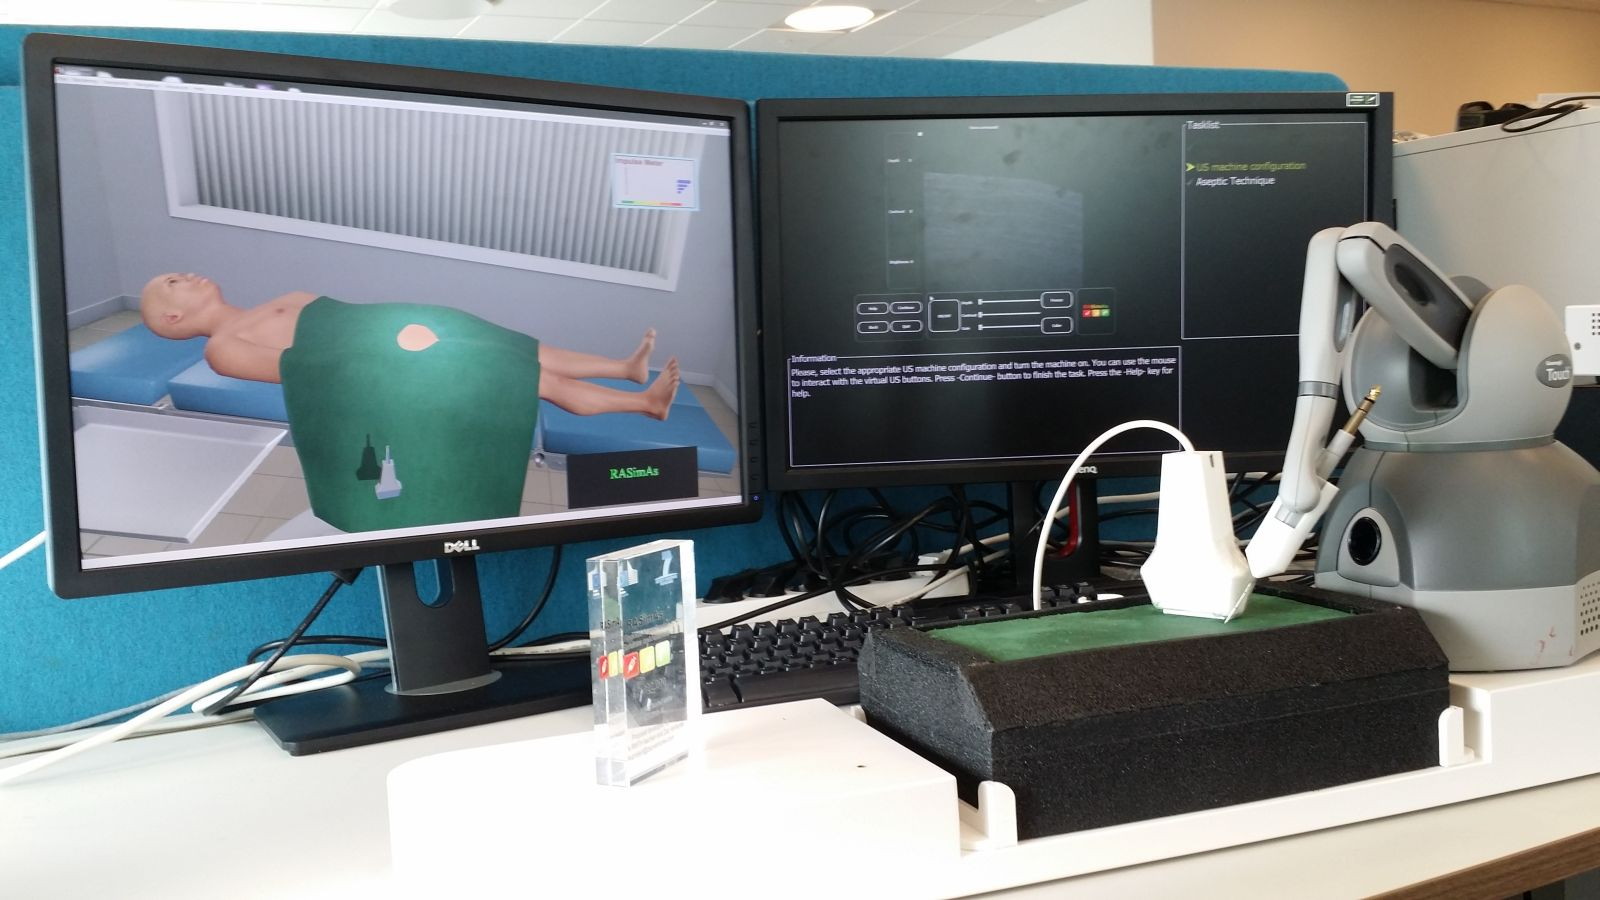
\includegraphics[width=1\textwidth]{IMG/sim3.jpg}
    \caption{RASim \label{subfig:introrasim}}
  \end{subfigure}%
  \begin{subfigure}[b]{0.5\linewidth}
    \centering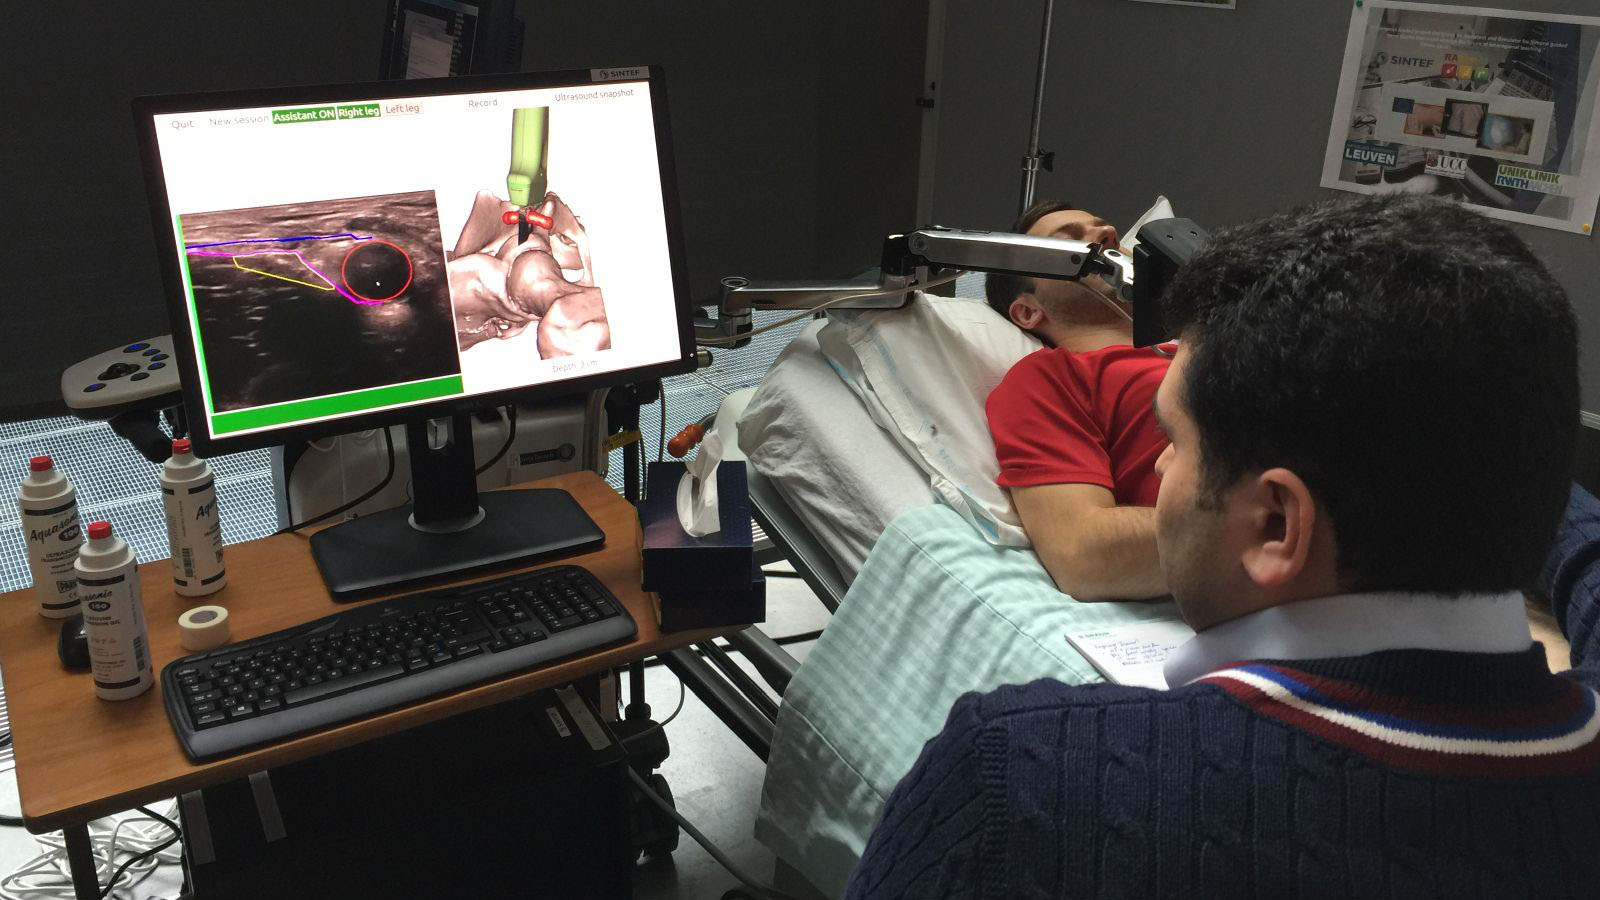
\includegraphics[width=1\textwidth]{IMG/raas.JPG}
    \caption{RAAs \label{subfig:introraas}}
  \end{subfigure}
  \caption{ Both RASimAs prototypes.}
\end{figure}



% %\todo{en pasado o presente?, pasado esta bien.}
% Esta tesis ha sido desarrollada dentro del contexto del proyecto \emph{RASimAs}, financiado por el 7º Programa del Marco de la Unión Europea. El objetivo principal es el desarrollo de herramientas que faciliten el entrenamiento y la práctica de la anestesia regional. Para cumplir con este objetivo se ha propuesto dos sistemas: un entrenador de realidad virtual llamado \emph{Regional Anaesthesia Simulator (RASim)} y un asistente en quirófano llamado \emph{Regional Anaesthesia Assistant (RAAs)}.

With the goal of facing a vast of anatomic variation, this project has proposed the development of a Virtual Physiological Human (VPH) database which it would be used in the \emph{RASim} simulator. An Integrated Toolkit for Generation of VPH Models (ITGVPH) has been developed for the generation of virtual patients based on patient-specific data. Additionally, it is required to transform the VPH models to the position required by the RA procedure. \emph{GMRV} group of the  \emph{Universidad Rey Juan Carlos} has been designated to lead this task.

% Con el objetivo de enfrentar a los médicos a la mayor cantidad de variabilidad anatómica posible, en este proyecto se ha propuesto desarrollar un entorno integrado de generación de pacientes virtuales, que permita crear una base de datos de modelos anatómicos que pueda ser utilizado por el simulador \emph{RASim}. Esta herramienta genera pacientes virtuales (VPH), a partir del registro de un modelo virtual con imágenes de pacientes reales. Además, es necesario transformar la postura del paciente generado a las diferentes posiciones requeridas por el procedimiento de anestesia regional. En concreto, esta tarea ha sido designada al grupo \emph{GMRV} de la \emph{Universidad Rey Juan Carlos}, estableciendo la motivación principal de esta tesis.

This thesis introduces a new technique that allows positioning the virtual patient models to the required position of the medical procedure. This new method works even if the virtual patient is incomplete or even if the mechanical model of the different tissues are not available. For this reason, it will be supervised by qualified physicians through a 3D UI. Therefore, the process must be interactive. To meet those requirements, a geometrically based approach have been followed. On the contrary, the physically based approach is not suitable because it needs a complete and proper model with the tissues' mechanic descriptions. Also, as they get accurate transformations, they required complex calculations that prevent interactive rates. Geometrical approaches provide plausible poses for training and educational purposes.

% A lo largo de este trabajo, se presenta una nueva técnica que permite transformar los modelos anatómicos de pacientes virtuales de su postura original a la posición necesaria por el procedimiento médico. Esto es posible aunque los modelos anatómicos se encuentren incompletos o falten sus descripciones mecánicas. Además, ya que el usuario supervisará la deformación que se aplicará al paciente virtual, el sistema debe tener tasas de refresco interactivas. Para cumplir con estos requisitos, se ha desarrollado una técnica geométrica basada en el cauce de la animación esqueletal, en lugar de utilizar un método basado en física debido a que estos últimos presentan una serie de problemas. En estos casos, se requiere caracterizar mecánicamente los tejidos que se van a simular los cuales no siempre se encuentran disponibles. Además, los métodos basados en modelos físicos se centran en conseguir deformaciones precisas, resultando en un alto grado de complejidad que impide conseguir tasas de refresco interactivas. Frente a los métodos basados en física, se ha optado por utilizar una técnica geométrica que proporciona soluciones plausibles que el usuario pueda interpretar como reales.

The proposed algorithm extends the classical skeletal animation pipeline to deal with character's internal tissues. From the skin and bones, our approach computes a displacement field from the bones’ movement, and uses it to transform the virtual tissues. Most of the complex tasks are computed during a pre-process stage, allowing to run the pose selection phase at interactive rates. It is fully automatic and it does not need users intervention.  Additionally, in order to refine the solutions, it was proposed an optimisation stage which uses a physically based approach in order to improve the volume conservation to achieve more appealing results. The figure \ref{fig:summaryarq} depicts the proposed animation pipeline stages. 



\begin{figure}[ht]
    \centering
    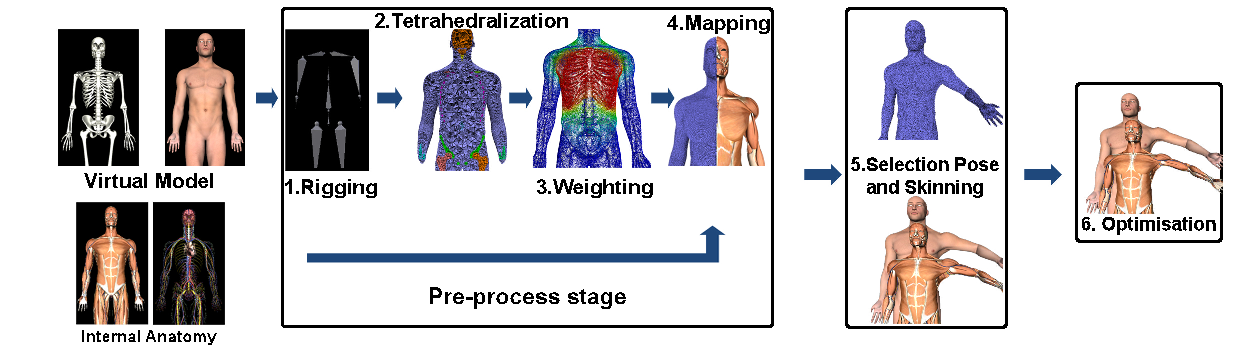
\includegraphics[width=0.95\textwidth]{IMG/summaryarq.pdf}
    \caption{Algorithm overview. First 4 steps represent the pre-process stage, Selection Pose and Skinning steps run at interactive rates and Optimisation phase is optional.}
    \label{fig:summaryarq}
\end{figure}

The following hypothesis has been formulated: "\emph{it is possible to create a geometrical algorithm which allows to transform the virtual patient pose with their internal tissues in order to use them in the context of medical training.}"  To validate it, two use cases have been developed.
% Partiendo de la piel y el tejido óseo del paciente virtual, se genera un campo de desplazamientos continuo en el interior del paciente virtual que se utiliza para transformar sus estructuras internas. Las operaciones más costosas se han delegado a un proceso previo que genera toda la información necesaria para que el usuario pueda seleccionar la postura del paciente virtual interactivamente. Además, se ha propuesto un refinamiento opcional basado en un método físico que intenta conservar el volumen del modelo anatómico. Con el objetivo de validar la hipótesis por la cual un algoritmo geométrico puede generar nuevas posturas de un paciente virtual junto con sus tejidos internos para ser utilizadas en el contexto del entrenamiento de un procedimiento médico, se han propuesto dos casos de uso. 


First, the proposed technique has been integrated into the ITGVPH, where it allows physicians to interactively animate a virtual patient. In this scenario, our algorithm works without complete models or mechanic properties. The pre-process stage must be performed once per model, but it automatically runs the complex steps avoiding the need of people with technical skills. Additionally, in order to prove the usefulness of those VPH in RA training, a courseware for the RASim simulator has been created. It provides a self-directed learning platform where trainees can rehearsal the procedure and improve their theoretical and non-cognitive skills. Courseware manages all simulation modules of RASim in order to develop training tasks. Unfortunately, haptic devices register manufacturing defects which made impossible to conduct a proper clinical trial of the simulator.

% En primer lugar, el algoritmo propuesto se ha integrado en el entorno de generación de pacientes virtuales, permitiendo animar y adaptar al profesional médico los modelos anatómicos generados por la suite. Se intenta demostrar que el algoritmo puede adaptar la postura de un modelo anatómico en un escenario donde no se dispone de modelos completos y no se dispongan de sus propiedades mecánicas. Además, con la finalidad de comprobar si los pacientes virtuales son útiles para  el entrenamiento del procedimiento de RA, se ha contribuido en la creación del módulo Courseware. Esta plataforma de aprendizaje donde el usuario podrá practicar y desarrollar sus habilidades no cognitivas, gestiona todos los componentes del simulador y se encarga de implementar las tareas de entrenamiento. Por problemas de precisión de los dispositivos hápticos, no se ha podido realizar una evaluación clínica del simulador. 
\begin{figure}[ht]
    \begin{subfigure}[b]{0.32\linewidth}
        \centering
        {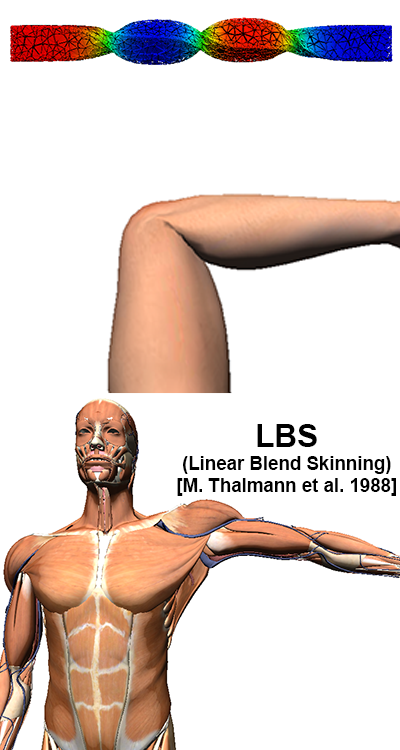
\includegraphics[width=\linewidth]{IMG/sLBS.png}}
        \caption{Bar model and \emph{ZygoteBody}$^{TM}$ transformed using linear blend skinning \label{subfig:sLBS}}
    \end{subfigure}
    \null\hfill
     \begin{subfigure}[b]{0.32\linewidth}
        \centering
        {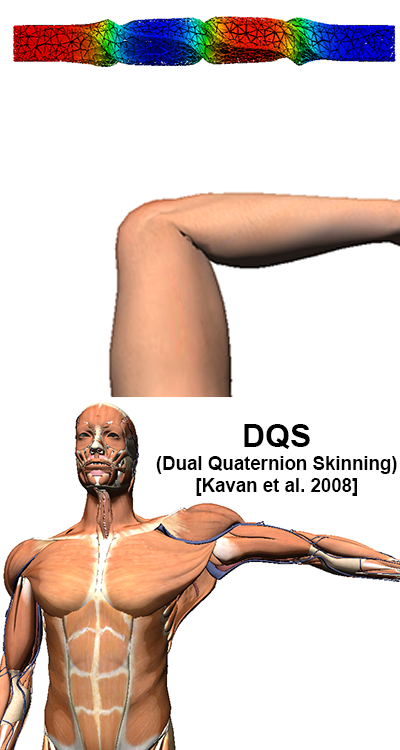
\includegraphics[width=\linewidth]{IMG/sDQS.png}}
        \caption{Bar model and \emph{ZygoteBody}$^{TM}$ transformed using dual quaternion skinning  \label{subfig:sDQS}}
    \end{subfigure}
    \null\hfill
     \begin{subfigure}[b]{0.32\linewidth}
        \centering
        {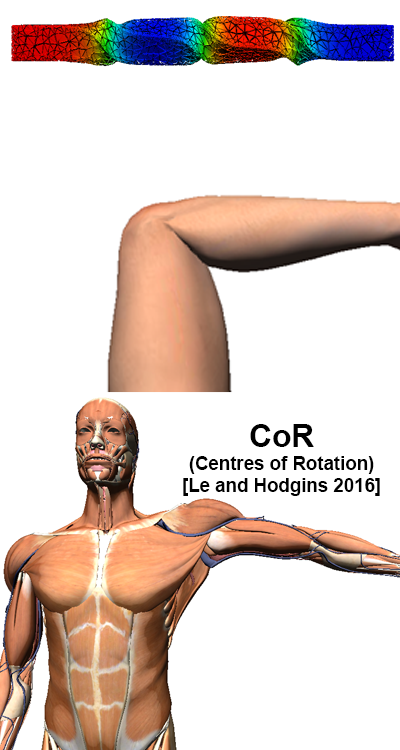
\includegraphics[width=\linewidth]{IMG/sCOR.png}}
        \caption{ Bar model and \emph{ZygoteBody}$^{TM}$ transformed using centres of rotation \label{subfig:sCOR}}
    \end{subfigure}
    \caption{\label{fig:compsummary} Some results obtained with three skinning techniques.}
   \end{figure}
Second, a projectional radiography simulator has been developed working closely with \emph{Dr. Franck P.Vidal}.   Projectional radiography (also called projection radiography, and X-ray radiography) is a very common medical imaging tool that supports clinicians in the diagnostic of certain diseases, infections, injuries (e.g.~bone fractures). Along the body, each specific location requires a correct patient positioning and X-ray machine configuration. Important aspects such as a convenience anatomic placement, collimation of the X-ray source, voltage of the X-ray tube, time of exposure, distance source to patient, and distance source to detector or film, must be dominated by radiographers in order to safely perform the procedure in a clinical environment. The simulator relies on the proposed technique and a real-time framework for the simulation of X-ray images provided by \emph{gVirtualXRay}\cite{sujar:hal}. Our method enables a user to pose interactively the virtual patient while \emph{gVirtualXRay} generates the corresponding X-ray image. Additionally, the proposed algorithm allows adding any external virtual patient model with the execution of the pre-process stage.  %The overall results  show that our tool is mostly realistic, useful and suitable in teaching and/or learning X-ray radiography.    

% En segundo lugar, se ha desarrollado un simulador de radiología diagnóstica gracias a la librería \emph{gVirtualXRay} en colaboración con \emph{Dr. Franck P.Vidal}. En este procedimiento, el médico debe posicionar al paciente y configurar la máquina de rayos X de manera que la región anatómica objetivo sea adecuadamente capturada. El algoritmo propuesto demuestra su capacidad para transformar la postura de un paciente virtual interactivamente, y así probar distintas proyecciones, mientras que la librería \emph{gVirtualXRay} permite  obtener imágenes de rayos X simultáneamente. Se ha realizado una encuesta a especialistas en radiología para comprobar su validez aparente y de contenido, donde se ha preguntado acerca de su opinión sobre el realismo y la utilidad del simulador. Los resultados obtenidos confirman su beneficio como herramienta adicional a las técnicas clásicas de aprendizaje.


Tests have been performed in order to evaluate the presented technique. In terms of performance, the preprocess take less than 7 minutes with the more complex virtual patient and it gets above 50 fps in the selection pose stage. For example, \emph{ZygoteBody}$^{TM}$ male model has close to $8 \times 10^5$ of vertices and $1.5\times 10^6$ of triangles; and produces an internal tetrahedral mesh which has close to $3.5\times 10^6$ of tetrahedrons and $8 \times 10^5$ of nodes.  Regarding the selected skinning technique, the two most used techniques are linear blending skinning (LBS) \cite{thalmann88} and dual quaternion skinning (DQS) \cite{Kavan2008}. They have been used, together with the new proposal which calculates optimal centres of rotation (COR) \cite{le2016real} for each vertex, by the algorithm to generate the results (see figure \ref{fig:compsummary}). 

In relation to ITGVPH, the proposed technique can work with incomplete models which come from this toolkit. For example, the figure \ref{fig:summarypatient} shows an incomplete model generated by ITGVPH with only the skin and bones, adapted by the proposed technique.
\begin{figure}[htbp]
    \centering
    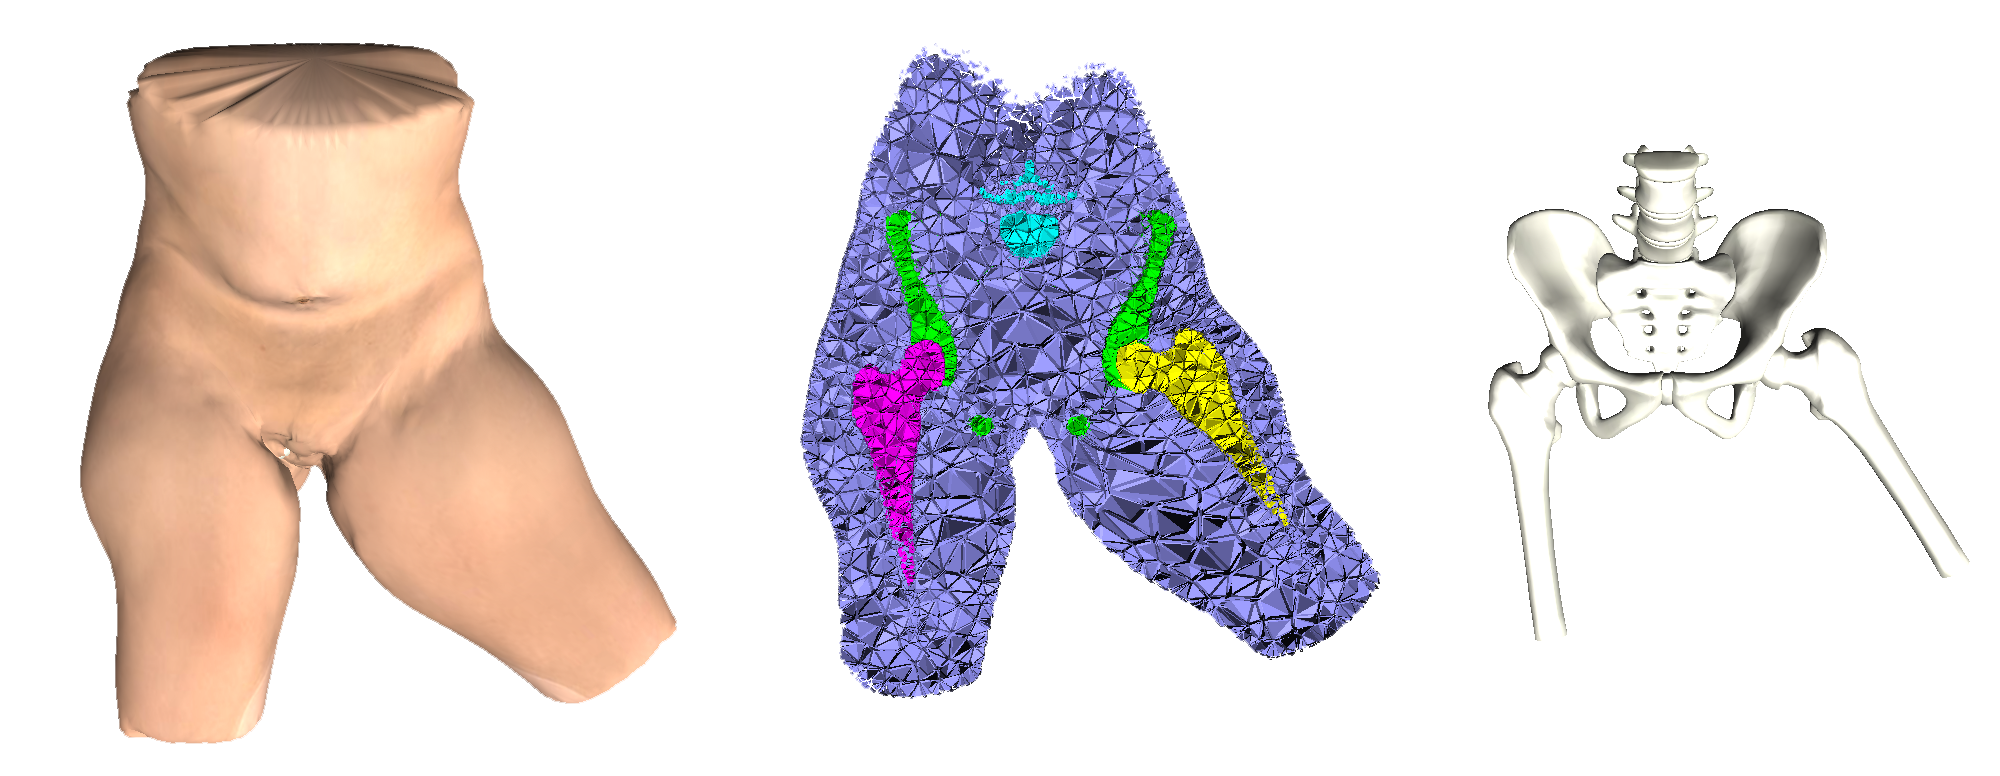
\includegraphics[width=0.95\textwidth]{IMG/spatient.png}
    \caption{Virtual patient model generated by ITGVPH and animated by the proposed technique.}
    \label{fig:summarypatient}
\end{figure}

Regarding the X-ray simulator (see fig. \ref{fig:summaryxray}), our algorithm together with \emph{gVirtualXRay} can run interactively above 25 fps and it could generate a variety of x-ray image from the input virtual patients. A promising face and content validation study have been conducted to gather  experts feedback. On one hand, the face validity performed shows that our tool is realistic in many ways.
The content validity performed shows both the usefulness and suitability of our tool in teaching and/or learning X-ray radiography. 



It is important to highlight that our geometric approachprovides a heuristic solution. Students do not need a specific patient model but a set of plausible virtual patients. This could be used for training and educational purposes.

\begin{figure}[htbp]
    \centering
    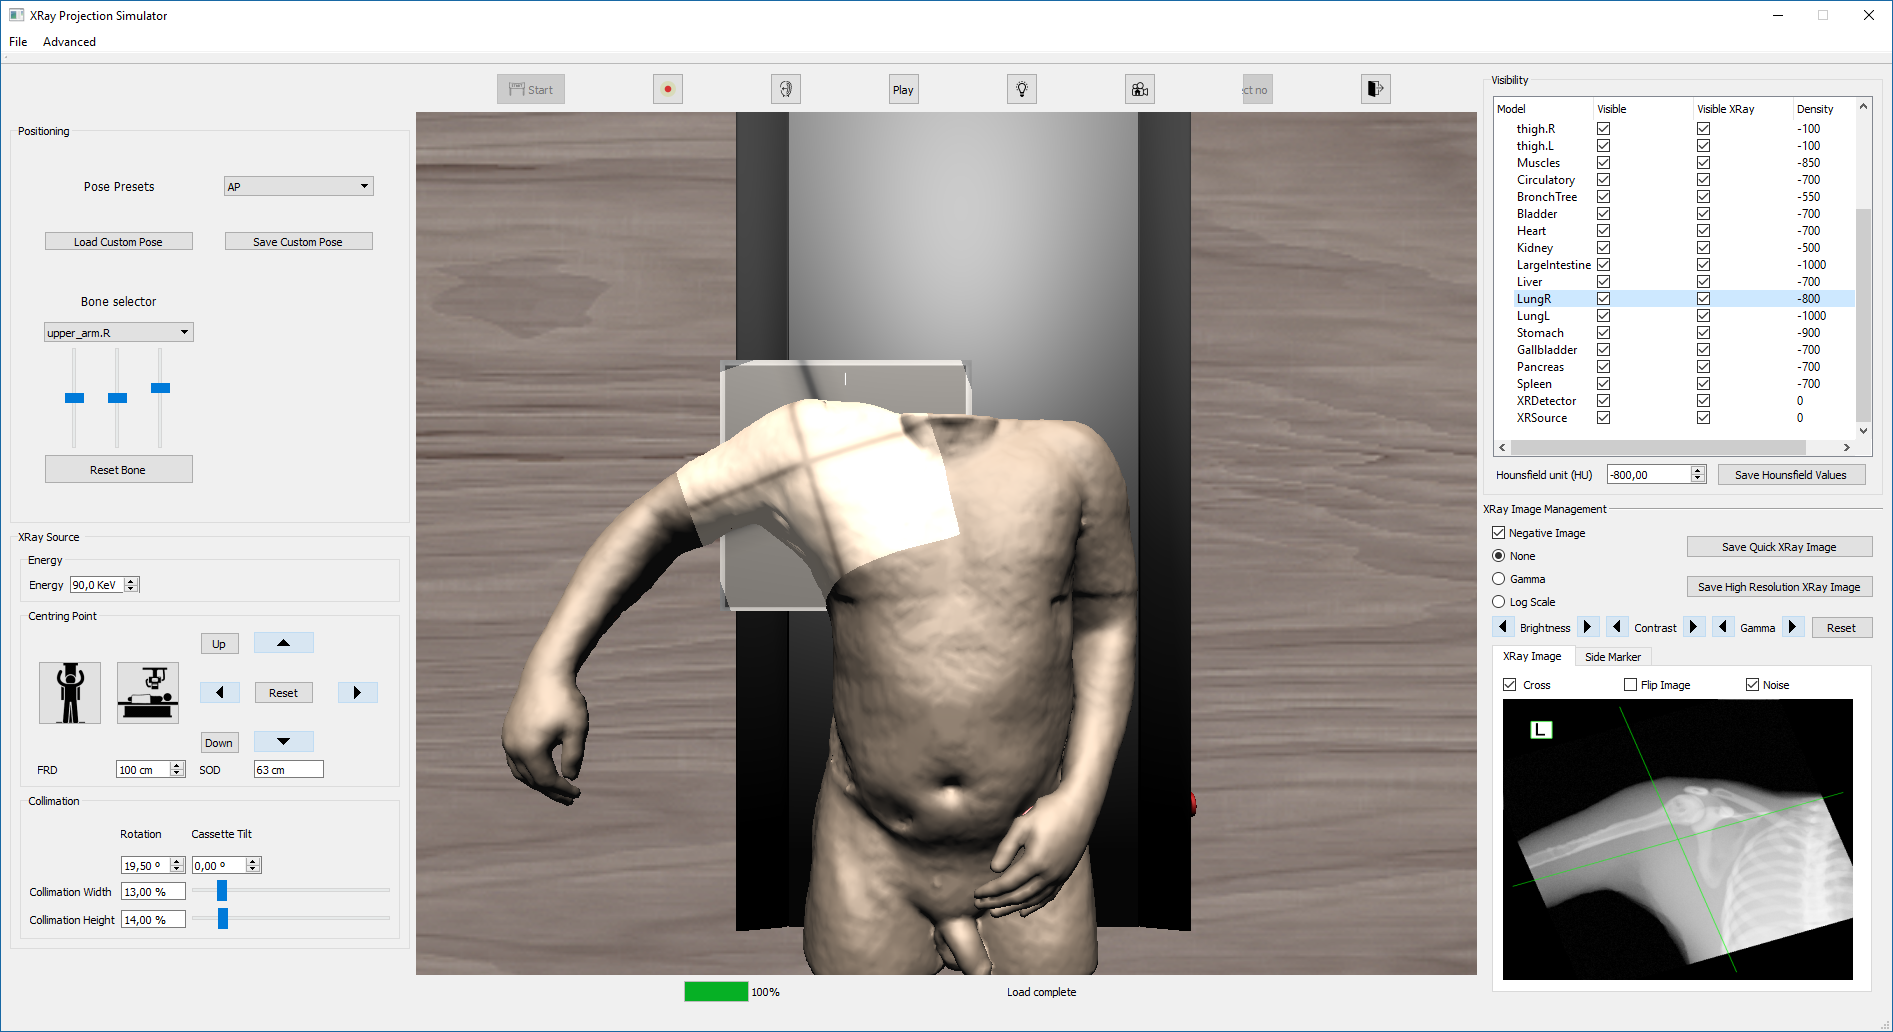
\includegraphics[width=0.95\textwidth]{IMG/suiteacher.png}
    \caption{UI of the X-ray simulator with the \emph{Segmented Inner Organs} \cite{VoxelMan}.}
    \label{fig:summaryxray}
\end{figure}

On one hand, it is worth to mention that the European Commission evaluated the \acs{RASimAs} project as \emph{Acceptable progress}. Although clinical trials were not conducted because of unexpected problems, they valued positively the \acs{RASim} prototype.

On the other hand, we present an interactive learning environment to teach radiography using real-time interactive X-ray simulation and to enhance the learning process. Face and content validity show both the usefulness and suitability of our tool.
\renewcommand{\figurename}{Figura}


%\thispagestyle{empty}
\chapter*{Lista de acrónimos}

\begin{acronym}
\acro{B-rep}{representación superficial}
\acro{Bangor}{Bangor University}
\acro{DQS}{dual quaternion skinning}
\acro{CAD}{diseño asistido por computador}
\acro{CGAL}{Computational Geometry Algorithms Library}
\acro{COR}{centros de rotación}
\acro{Courseware}{aplicación de entrenamiento}
\acro{DICOM}{Imagen y Comunicación Digital en Medicina}
\acro{DOF}{grados de libertad}
\acro{E/S}{Entrada/Salida}
\acro{EASA}{Agencia Europea de Seguridad Aérea}
\acro{FEM}{método de elementos finitos}
\acro{FORTH}{Foundation for Research and Technology - Hellas}

\acro{GLSL}{OpenGL Shading Language}
\acro{GMRV}{Grupo de Modelado y Realidad Virtual}
\acro{GPL}{GNU General Public License}
\acro{GPU}{unidad de procesamiento gráfico}
\acro{INRIA}{Institut National de Recherche en Informatique et en Automatique}
\acro{IRM}{imagen por resonancia magnética}
\acro{ITGVPH}{Integrated Toolkit for Generation of VPH Models}
\acro{IU}{interfaz de usuario}
\acro{joints}{articulaciones virtuales}
\acro{keV}{kiloelectronvoltios}
\acro{kV}{kilovoltios}
\acro{kVp}{tensión de pico}
\acro{LBS}{linear blending skinning}
\acro{LGPL}{GNU Lesser General Public License}
\acro{mAs}{miliamperios por segundo}
\acro{MoCap}{captura de movimientos}
\acro{RA}{anestesia regional}
\acro{RAAs}{Regional Anaesthesia Assistant}
\acro{RAM}{Random Access Memory}
\acro{RASim}{Regional Anaesthesia Simulator}
\acro{RASimAs}{Regional Anaesthesia Simulator and Assistant}
\acro{RDT}{triangulación restringida de delaunay}
\acro{RV}{realidad virtual}
\acro{RWTH}{RWTH Aachen University}
\acro{SBS}{Spherical Blend Skinning}
\acro{SINTEF}{Stiftelsen for industriell og teknisk forskning}
\acro{SG}{Sensegraphics}
\acro{SOFA}{Simulation Open Framework Architecture}
\acro{tabla hash}{Spatial Hash Table}
\acro{TASMIP}{Tungsten anode spectral model using interpolating polynomials}
\acro{TC}{tomografía axial computarizada}
\acro{TPTVPH}{Toolkit for Pose Transforms of VPH Models}
\acro{tracker}{dispositivo de seguimiento}
\acro{UKA-IMI}{Department of Medical Informatics: Uniklinik RWTH Aachen}
\acro{URJC}{Universidad Rey Juan Carlos}
\acro{US}{ultrasonidos} 
\acro{ViSTA}{Virtual Reality Toolkit}
\acro{VPH}{pacientes virtuales}
\acro{VTU}{formato de Visualization Toolkit}
\acro{WP}{paquetes de trabajos}
\acro{X3D}{formato Extensible 3D}
\acro{XML}{Extensible Markup Language}
\acro{ZPD}{zona de desarrollo próximo}













\end{acronym}


\tableofcontents


\listoffigures
 
\listoftables
\titleformat{\chapter}[hang]
  {\normalfont\bfseries}{}{0pt}{\huge\thechapter. }

\mainmatter

%%%% INTRODUCCiÓN


\chapter{Introducción} 
\label{cap:intro}


% \todo{Entiendo que quieres comentar la importancia de los gráficos por computador en el mundo actual. Primero te comento errores cometidos y luego te propongo soluciones:
% 1. La generación de imágenes hace referencia solo al proceso de renderizado. El área de conocimiento son los gráficos por computar, estos incluyen animación, modelado, post-proceso.
% 2. El mundo del la generaicón y tratamiento de imagenes es demasiado amplio. Tú deberías centrarlo en el campo del los gráficos 3D (aquellos en los que la imagen generada nos permite de alguna manera (claves perpetúales captar la profundidad))
% 3. Todo el mundo sabe que los gráficos 3D estan tanformando el mundo del ocio (peliculas de animación, videojuegos) y el mundo profesional (por cierto no hablaria del mundo profesional, hablaria de la cientcia, el foramción, analisis de datos, interacción hombre máquina ...). Pero en este párrafo no concretas estas aportaciones. Ocio: ciene y videojuegos, Apredizaje: gamificación, entremiento en entornos seguros. Ciencia: Visualización y análisis de datos.... 
% Solución:
% No hables de los graficos por computador. Tu tesis se enmarca en la RV. La RV utiliza los graficos por computador y muchas otras displinas. 
% Te estoy metiendo comentarios largos por si te pueden ayudar con futuras redacciones. }

Durante los últimos años, el término de \ac{RV} se ha incorporado a nuestro lenguaje cotidiano. Esto es debido a la gran penetración que están teniendo este tipo de sistemas en nuestra vida privada y, cada vez más, en distintos ámbitos profesionales. Se pueden encontrar ejemplos de estas aplicaciones en sectores tan diversos como: el mundo del ocio, donde los videojuegos son el máximo exponente del uso de estas tecnologías; el campo del entrenamiento profesional, en el que la \ac{RV} permite el desarrollo de destrezas no cognitivas en entornos controlados \cite{PATEL2017266.e7}; el ámbito científico, donde estos sistemas facilitan la compresión de datos complejos mediante el uso de entornos inmersos \cite{usher2018}. Dado el gran número de campos de aplicación y de tecnologías utilizadas, no resulta fácil indicar de forma unívoca qué caracteriza una aplicación de \ac{RV}. En la bibliografía, se pueden encontrar distintas definiciones del término:

\begin{center}
    \begin{minipage}{0.9\linewidth}
        %\vspace{5pt}%margen superior de minipage
        {\small
\emph{Virtual reality is a high-end user-computer interface that
involves real-time simulation and interactions through
multiple sensorial channels.}
        }
        \begin{flushright}
            (Burdea y Coiffet, 2003: \cite{burdea2003virtual})
        \end{flushright}
        %\vspace{5pt}%margen inferior de la minipage
    \end{minipage}
    
    \begin{minipage}{0.9\linewidth}
        %\vspace{5pt}%margen superior de minipage
        {\small
\emph{VR is the science and technology required for a user
to feel present, via perceptive, cognitive and functional
immersion and interaction, in a (computer) generated
environment. }
        }
        \begin{flushright}
            (Casarin et al., 2015: \cite{kuntz2015middlevr})
        \end{flushright}
        %\vspace{5pt}%margen inferior de la minipage
    \end{minipage}
    
\end{center}
%
%\todo{1.La realidad virtual no es una subcampo del los graficos por computdor.2.En algún lugar hay que hablar de la multidisciplinaridad de este campo (ingeniería, ciencias de la computación, psicología, graficos por computador...). Puede ir despues de la definición.}
% Este comentario esta para que no sea un parrafo nuevo
Tal y como se desprende de las definiciones anteriores, las aplicaciones \ac{RV} se caracterizan por presentar al usuario un entorno virtual a través de varios canales sensoriales, permitiéndole interactuar con el mismo y generando en él, una sensación de inmersión y presencia \cite{Jerald:2015}. Estos objetivos imprimen a este campo una naturaleza altamente multidisciplinar. La \ac{RV} se asienta en disciplinas como la ingeniería mecánica, los gráficos por computador, la percepción, la computación de altas prestaciones, etcétera. De esta forma, el desarrollo de estas aplicaciones requiere naturalmente de expertos en distintas áreas de conocimiento.  

%\todo{ojo con afirmar cosas que no estan justificadas como "inmersión completa" o "todos los sentidos"}

El auge de la \ac{RV} es evidente, pudiéndose encontrar multitud de aplicaciones en campos tan diversos como el arte, el marketing, la psicología, el diseño y prototipado..., siendo los sectores del entrenamiento de profesionales (de muy diversa naturaleza) y del ocio, en los que más se ha desarrollado.

%\todo{1. Es importante en las 2. 2. En lugar de decir que los entrenadores virtuales son de gran importancia, di que es donde se enmarca este trabajo de tesis.3. Explica las ventajas frente a los métodos clasicos. Es en esta última, donde la \ac{RV} tiene una gran importancia ya que se ha podido comprobar que puede traer grandes beneficios en la enseñanza y aprendizaje utilizando las nuevas tecnologías de manera atractiva frente a los métodos clásicos.}
Esta tesis se centrará en el ámbito de las aplicaciones de \ac{RV} con fines de entrenamiento de profesionales en tareas complejas. En muchas profesiones, existen procesos que requieren destrezas no cognitivas que solo pueden adquirirse mediante la práctica, siendo necesario recurrir a técnicas de entrenamiento alternativas y, especialmente, cuando la actividad entraña un riesgo para el profesional o para terceros. En estos casos, las aplicaciones de \ac{RV} han demostrado  grandes ventajas sobre las técnicas de entrenamiento tradicional~\cite{PATEL2017266.e7}, proporcionando un entorno seguro, repetible y variado en los escenarios donde los usuarios pueden practicar. A pesar de ello, el desarrollo e implantación de estos sistemas no está exento de dificultades. Se deben diseñar (con una correspondiente evaluación a posteriori) de forma que las destrezas que se pretenden adquirir sean transferibles del entorno virtual al mundo real. Además, es importante garantizar que no se adquieran malos hábitos o destrezas solamente válidas en el contexto del simulador.

Dicho esto, uno de los campos donde los entrenadores virtuales han penetrado con más fuerza, es el de la aviación \cite{lee2017flight}. Los simuladores de vuelo son una herramienta esencial que forma parte del currículum de los nuevos pilotos comerciales \cite{piloto}. El objetivo de estas herramientas no es solo de entrenamiento, sino que también proporcionan una plataforma de evaluación.  %\todo{Aaron intenta ser un poco más formal: Concretamente la EASA (poner en tu lista de acrónimos) establece el uso del simulardores de vuelo en curriculum de los futuros pilotos comerciales como un requisito para obtener su licencia}
Concretamente, la \ac{EASA} establece el uso de los simuladores de vuelo en el currículum de los futuros pilotos comerciales como un requisito para obtener su licencia \cite{normativa}.
%\todo{Busca si es por ley y cambia la frase}.

%\todo{Aaron te lo he cambiado para que suene más formal. Cuando metas una frase léelo 2 veces para ver si puede hacer que suene mejor}
Por otra parte, otro campo donde son evidentes los beneficios de la \ac{RV} es  el ámbito médico. Un ejemplo claro son las prácticas quirúrgicas donde se requiere de la manipulación mecánica de estructuras anatómicas. De este modo, el entrenamiento de dichos procedimientos se caracteriza por tener un alto componente práctico, de cara a adquirir las destrezas no cognitivas con las que asegurar que en el futuro se procederá de manera efectiva y segura.
%\del{Por otra parte, en el ámbito médico, la prácticas quirúrgicas requieren de la manipulación se encarga de la curación del paciente mediante la manipulación mecánica de las estructuras anatómicas y por ende su aprendizaje se caracteriza por un gran componente práctico.}
Es por ello que, dado el riesgo que suelen representar este tipo de técnicas para los pacientes, este campo está especialmente interesado en el desarrollo de nuevas metodologías que den la posibilidad de entrenar en entornos seguros, repetibles y variados. Por este motivo, en los últimos años siguen proliferando trabajos académicos que proponen nuevos simuladores médicos de \ac{RV}~\cite{korzeniowski2018vcsim3,cecil2017advanced}. En la actualidad, la nueva generación de simuladores quirúrgicos va encaminada a desarrollar las capacidades de aprendizaje autónomo, evaluación de capacitaciones y planificación de intervenciones. A pesar de ello, estas aplicaciones aún no son comunes en el currículum de las distintas especialidades médico/quirúrgicas y la implantación de este tipo de herramientas todavía debe superar un gran número de retos tecnológicos, éticos y legales. A continuación, se han listado algunos de los más importantes:
\begin{itemize}
    \item Diversidad de procedimientos: existen infinidad de procedimientos médicos diferentes entre sí, que se caracterizan por utilizar instrumental específico y, además, donde se trabaja en áreas y sobre estructuras anatómicas diferentes. Esta situación dificulta el desarrollo de soluciones de propósito general.
    \item Limitaciones en los dispositivos \ac{E/S}: muchas técnicas quirúrgicas requieren de la correcta interpretación de estímulos visuales, propioceptivos y táctiles. Actualmente, los dispositivos E/S existentes están muy limitados a la hora de presentar este tipo de información al usuario. 
    \item Simulación de fenómenos físicos complejos con tasas de refresco y latencias interactivas: en muchas ocasiones, no se pueden simular físicamente las interacciones mecánicas en tiempos interactivos. Además, la complejidad aumenta al añadir la diversidad de tejidos y fenómenos naturales que deben contemplarse. 
    \item Dificultad de obtener modelos anatómicos adecuados: en la actualidad, ninguna técnica de imagen médica (\ac{US}, \ac{TC}, \ac{IRM}, etcétera) es capaz de obtener descripciones completas de un paciente \cite{mita}. Por otro lado, las imágenes obtenidas deben adaptarse a representaciones que puedan utilizarse durante la simulación.
\end{itemize}
%\todo{creo que los dos últimos puntos son importantes de cara a justificar objetivos}

Es importante indicar que el objetivo del listado anterior no es enumerar de forma precisa las líneas de trabajo actuales en este campo, sino que se busca ayudar al lector a entender algunos de los motivos que explican por qué la \ac{RV} aún no forma parte del programa docente de la mayoría de las especialidades quirúrgicas, a pesar de sus evidentes ventajas. En esta tesis, se ha trabajado en proponer soluciones que alivien algunos de los problemas derivados de los dos últimos puntos del listado anterior.



% \del{En este sentido, los simuladores de \ac{RV} proporcionan una importante herramienta de aprendizaje en muchos ámbitos\todo{separa en frases}, siendo el máximo exponente los simuladores de vuelo, \del{entre otros,} ya que están totalmente integrados dentro de la formación de un profesional de la aviación}\todo{La idea es que algunos entrenadores estan tan maduros que forman parte de currículum formativo de algunas profesiones. Estos simuladores proporcionan un entorno de seguro que no entraña riesgos ni personales ni materiales y fácilmente repetible. De ello surge que estos sean los aspectos más buscados en el ámbito de la medicina, dónde los simuladores han crecido de manera exponencial durante las últimas décadas.} \todo{esta bien las ideas pero mal el orden. Mal ligado con lo que cuenta en el párrafo anterior. Mas ventajas como la planficación. Esta idea tiene que esta muy desarrollada.}

% \del{
% En cuanto a los simuladores médicos, actualmente representan un gran reto en comparación con \new{otros entrenadores como}, los simuladores de vuelo o conducción, estando estos últimos más que establecidos . La gran variabilidad entre procedimientos médicos, variedad de instrumental médico y la complejidad del cuerpo humano son las variables que representan actualmente los problemas a los que se enfrentan estos tipos de simuladores.}\todo{Me parece superficial. simulación física y rendering en tiempo real. He intentado (desarrollar estas ideas.}

% \del{La utilidad de estos simuladores van más allá del simple aprendizaje del procedimiento sino que también en entrenar las habilidades no-cognitivas que son necesarias adquirir para interiorizar y generalizar el aprendizaje. Estos simuladores permiten transmitir esas habilidades del mundo virtual al mundo real.}\todo{cita. 2. Hay que garantizar que se aprende, que las destrezas adquiridas no son validad solo en el entorno del simalador, que no se adiquieren destrezas dañinas} \del{Incluso, también pueden ser usados para permitir la planificación previa de un determinado procedimiento o la evaluación de las aptitudes de los  profesionales médicos al igual que se realiza con los simuladores de vuelo.}\todo{Las ideas esta bien pero esta tratadas de forma un poco superficial y sin justificar. 2. Que se necesita para la planificación, que se necesita para la evaluación de competencias. 3. No me gustaba la estructura. Saltaba de alante atrás }

% \del{Las mejoras continuas en el rendimiento de computadores permiten cada vez más simulaciones físicas más realistas incluso, acompañadas del desarrollo de nuevos dispositivos periféricos, son por ello el principal motivo del auge de estos simuladores. Además de enfocarse en la calidad de la simulación, la comunidad científica y la industria también está centrada en ser capaces de llevar la información de pacientes reales a los simuladores, de tal forma que puedan ser utilizados datos reales en vez de modelos artificiales creados específicamente para el simulador.\todo{esta idea la has contado antes. Es importante no estar dando saltos de atrás-adelante}}


\section{Contexto}

De cara a comprender los objetivos que se plantean más adelante en el presente documento, es importante entender el contexto en el que se ha desarrollado la presente tesis. 
%\new{ Esto será explicado en los siguientes apartados:}\del{Este contexto, se explica en los subapartados redactados a continuación:}
Este contexto, se explica en los subapartados redactados a continuación.


\subsection{El proyecto RASimAs}
\label{intro:rasimas}

Desde noviembre de 2013 hasta octubre del año 2016, el \ac{GMRV}, de la \ac{URJC}, participó activamente el proyecto \ac{RASimAs} \cite{rasimasweb}, financiado por el Séptimo Programa del Marco de la Unión Europea. En él participaron investigadores y profesionales de centros y empresas punteras de 10 países diferentes. El proyecto planteó, como objetivo principal, el desarrollo de herramientas que facilitasen el entrenamiento y la práctica de la \ac{RA}, reduciendo así los riesgos para el paciente. En concreto se propusieron dos sistemas: un entrenador de \ac{RV} llamado \ac{RASim}(fig.\ref{subfig:rasim}) y un asistente que debía entrar en quirófano \ac{RAAs}(fig.\ref{subfig:raas}). Esta tesis se enmarca en el desarrollo del primer sistema.

\begin{figure}[ht]
  \centering
  \begin{subfigure}[b]{0.5\linewidth}
    \centering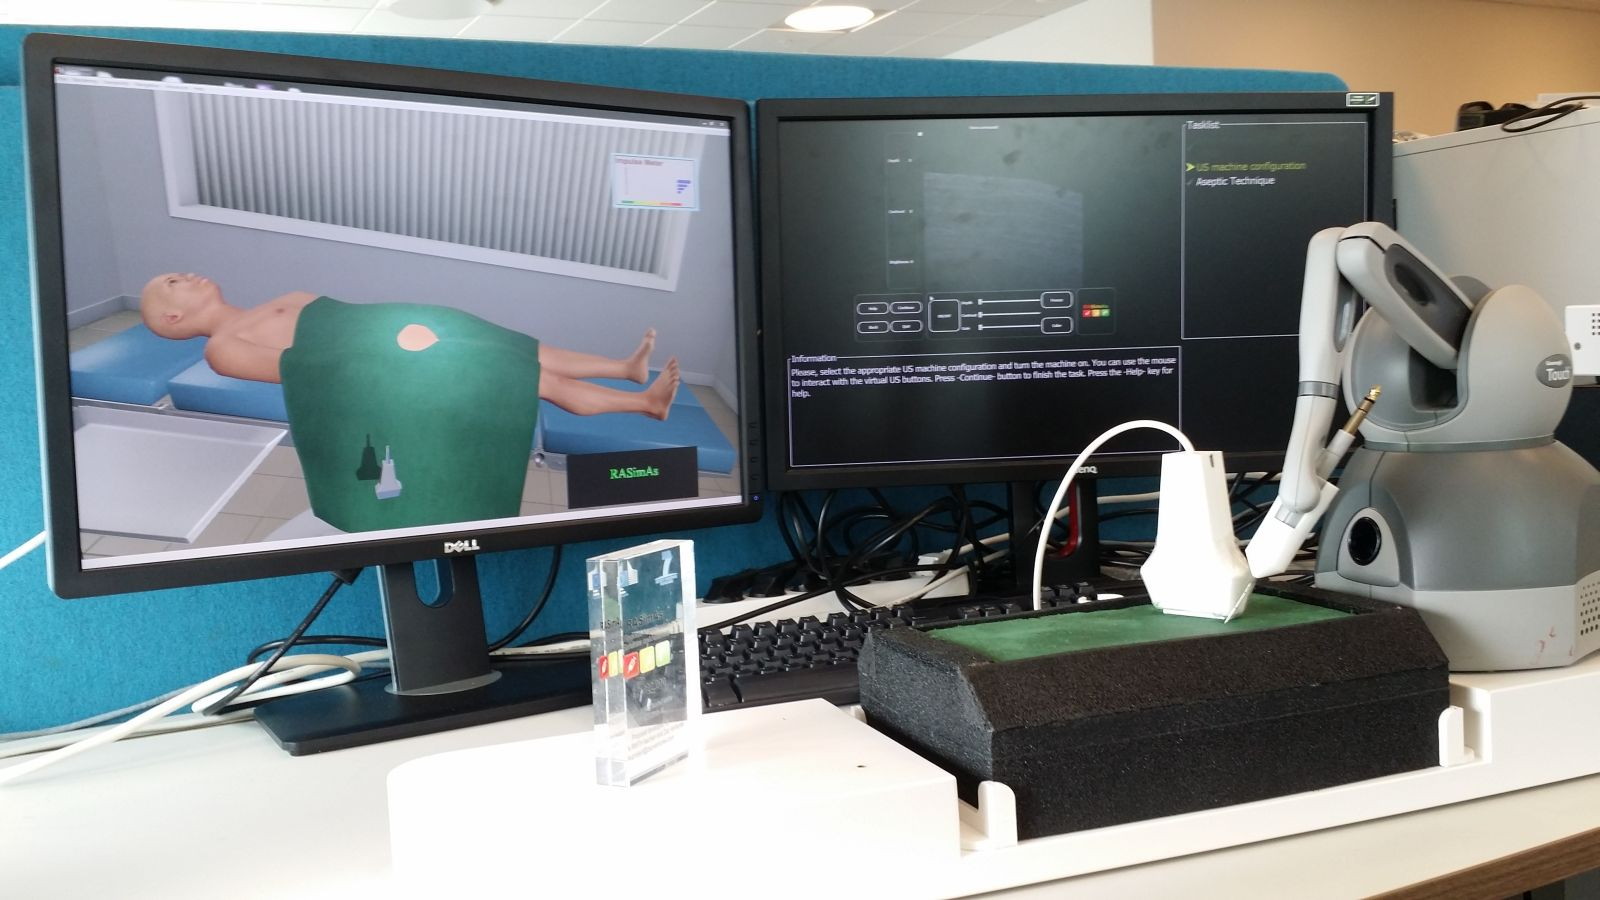
\includegraphics[width=1\textwidth]{IMG/sim3.jpg}
    \caption{\acs{RASim} \label{subfig:rasim}}
  \end{subfigure}%
  \begin{subfigure}[b]{0.5\linewidth}
    \centering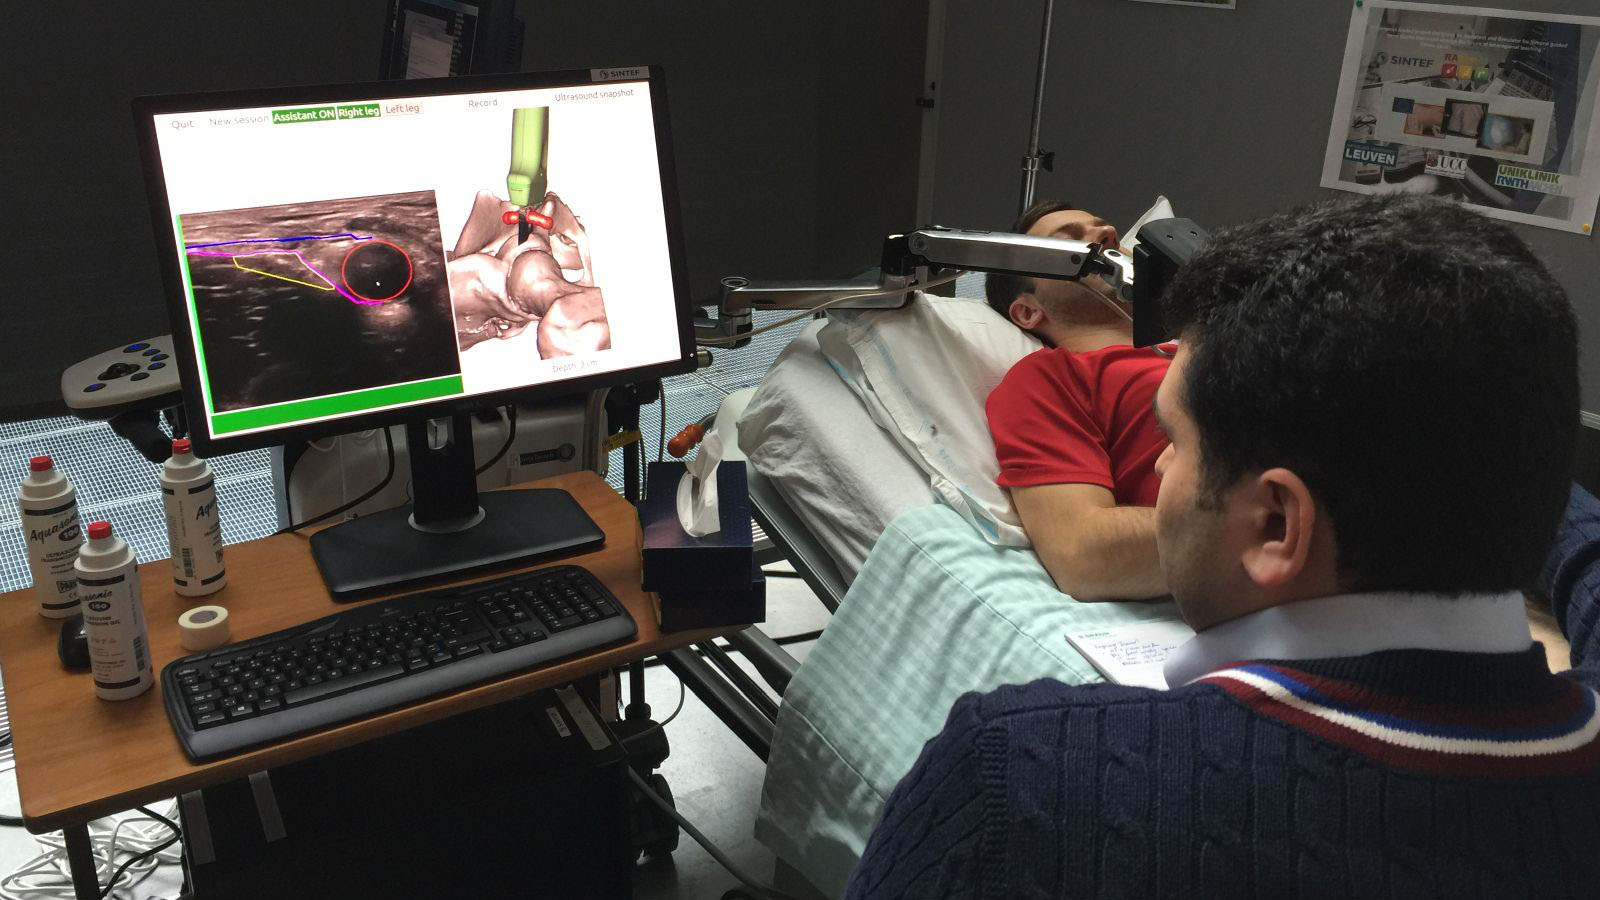
\includegraphics[width=1\textwidth]{IMG/raas.JPG}
    \caption{\acs{RAAs} \label{subfig:raas}}
  \end{subfigure}
  \caption{Imágenes que muestran los dos prototipos desarrollados en el contexto de \acs{RASimAs}.}
\end{figure}

%https://www.openanesthesia.org/regional-anesthesia-curriculum/
%http://rasimas.imib.rwth-aachen.de/member_area/documents_ma/Extra_Material/ISRA_Anaesthesia_Foundation_Course_Book_v1_to_print_for_ISRA_course_Oct_2_2014.pdf
%\todo{ Pon alguna cita, aquí y en el estado del arte. Por ejemplo, el CV de RA de Cork. Esto luego lo usaras en el courseware}

La \ac{RA} es un procedimiento mínimamente invasivo en el cual el médico administra un anestésico local en las proximidades del nervio que se desea bloquear \cite{CVraisra}. Esta técnica, frente a la anestesia general y si se practica adecuadamente, reduce: los efectos adversos sobre el paciente, su tiempo de recuperación y el coste de la intervención \cite{PMID:26695878}. La dificultad principal del procedimiento radica en liberar el bolo anestésico alrededor del nervio, sin tocarlo, evitando liberar la dosis en el torrente sanguíneo y confirmar que éste se ha extendido correctamente a su alrededor. Actualmente, existen dos técnicas para guiar la aguja hacia su objetivo: la estimulación eléctrica del nervio y el uso de imagen por \ac{US}. Aunque ambas técnicas pueden combinarse, la tendencia actual es abandonar la electroestimulación en favor del guiado por \ac{US}.

% \del{La \ac{RA} es un procedimiento médico dónde el \del{anestesiólogo}\new{anestesista!!!!!} administra anestésicos locales al paciente, a través de una aguja guiada por \ac{US} \todo{ojo hay otras formas de guiado. Tienes que ser muy preciso} en áreas cercanas a nervios específicos, produciendo una disminución de su actividad y ausencia del dolor. Esto posibilita la realización de cirugías sin necesidad de dormir al paciente completamente. De esta manera, se puede reducir el dolor postoperatorio, mejora la recuperación postoperatoria y se reduce el tiempo de hospitalización. De hecho, la anestesia regional se está imponiendo frente a la anestesia general debido a su menor coste e impacto en el paciente. \todo{cita}}
Sin embargo, esta técnica no es sencilla para los anestesistas que no están familiarizados con la ultrasonografía. Requiere tener una buena base teórica y práctica que permita proceder de manera segura. Hoy en día, está técnica se aprende principalmente practicándola sobre el paciente (\emph{by doing}), aunque existen otras técnicas como el uso de cadáveres \cite{Tsui2007} o \emph{fantomas}\footnote{Castellanización del término inglés Phantom.} \cite{phantomra}. Estas técnicas tienen claras limitaciones como: un alto coste,
la imposibilidad de repetir escenarios, el aprendizaje auto-guiado, 
que el usuario no se enfrente a una amplia variabilidad anatómica, etcétera.
%\borrar{enfrentar al usuario a una amplia variabilidad anatómica, etc.}

En primer lugar, \ac{RAAs} es un sistema de guiado que superpone información adicional sobre la imagen de \ac{US}, ayudando al usuario a identificar distintas regiones de interés. El sistema dispone de un \ac{tracker} y de un módulo de análisis de imagen que ayudan al médico a reconocer la aguja, la trayectoria de esta y las estructuras anatómicas relevantes mientras se está realizando la operación. 
% \del{Respecto a el sistema de guiado \ac{RAAs} consiste en asistir al anestesiólogo durante el procedimiento de \ac{RA}. Este sistema consta de unos dispositivos de seguimiento incorporados en la aguja y en la sonda del \ac{US}, de tal manera que con la información de seguimiento y la imagen de \ac{US}, el asistente proporcionará retroalimentación de inmediato que ayudará al médico a interpretar la imagen de \ac{US} de la anatomía del paciente.}


%\todo{Rehaz este parrafo. 1. No entiendo porque solo destacas 2 modulos del sistema el haptico y el fantoma. No has hablado del curseware, de las métricas del modo guiado. Del modulo físico, del modulo de ultrasonidos. Estructuralo todo en partes Hw y Sw y detallalas todas. } 
%
\ac{RASim} es un simulador médico que recrea un entorno de \ac{RA} donde el usuario puede entrenar el procedimiento. El usuario se sitúa en frente de la mesa de trabajo donde podrá encontrar: un maniquí y los dispositivos de \ac{E/S}.
El usuario interacciona con el sistema a través de una sonda de \ac{US}, con un \ac{tracker} magnético incorporado, y una aguja, acoplada a un dispositivo háptico. Estos dispositivos permiten al sistema seguir los movimientos del operador y proporcionar una respuesta háptica (en el caso de la aguja).
El usuario puede seguir el avance del procedimiento gracias a dos pantallas. En una, se muestra una vista virtual de la sala de operaciones  y, en la otra, se muestra la interfaz de la \ac{Courseware}\footnote{Software diseñado para fines educativos que sirve como ayuda o refuerzo del contenido.} con la imagen simulada de \ac{US}.
%
Así mismo, el simulador se compone de varios módulos software:
\begin{itemize}
    \item Módulo de respuesta háptica para la aguja.
    \item Simulación física entre los tejidos y los instrumentos médicos.
    \item Módulo de simulación de imágenes de \ac{US}.
    \item Renderizado de la escena virtual.
    \item Plataforma de autoevaluación y aprendizaje (\acs{Courseware}).
\end{itemize}

Es importante destacar que el módulo \ac{Courseware} es el que convierte al simulador en una plataforma de entrenamiento. Este software dirige al usuario a través del procedimiento mientras coordina todos los módulos del simulador en función del tipo de entrenamiento.  
%
El simulador permite practicar el procedimiento completo en un entorno seguro, además de mejorar sus habilidades cognitivas y no cognitivas gracias a la realimentación que proporciona el sistema.

Con el objetivo de enfrentar a los médicos a distintos escenarios que representen una variabilidad anatómica significativa, en el proyecto \ac{RASimAs} se ha propuesto desarrollar un entorno integrado de generación de pacientes virtuales (en inglés: \ac{ITGVPH}) con el que generar una base de datos de pacientes virtuales  que  podrán ser utilizados en \ac{RASim}. 
%
Esta herramienta genera \ac{VPH}, a partir del registro de un modelo virtual con imágenes de pacientes reales.
También es capaz de cambiar la postura inicial del paciente virtual a la posición requerida por el procedimiento y generar el comportamiento mecánico de los tejidos necesarios para su simulación física. Cabe destacar que los pacientes virtuales generados por esta herramienta no se corresponden con datos de pacientes reales, sino con variedades anatómicas representativas.
%\new{Por otra parte, este mismo sistema puede ser usado como plataforma de entrenamiento autoguiado en la que el usuario puede practicar el procedimiento gracias a la retroalimentación que el sistema proporciona.}

%Se ha diseñado una mesa de trabajo donde el usuario interacciona con el sistema. En ella, se encuentran dos pantallas que sirve para proporcionar información visual al usuario. En una de ellas se puede visualizar una vista de la sala de operaciones virtual y en otra, se muestra la vista del software de entrenamiento junto con la imagen simulada de \ac{US}. En la mesa de trabajo, el usuario maneja una sonda de \ac{US}, con un \ac{tracker} magnético incorporado, y una aguja, acoplada a un dispositivo háptico, que permite al sistema el seguimiento de los movimientos del usuario. El simulador es capaz de simular la interacción y deformación de los instrumentos y tejidos, y generar una imagen de \ac{US}. El \ac{Courseware} es el encargado de dirigir al usuario a través del procedimiento y gestionar todos los modulos del simulador. 

%\todo{tienes que restructurar toda la información de RASim. 1. Objetivos (no uses la palabra objetivos todo el rato):variabilidad anatómica gran base de datos de pacientes, aprendizaje autónomo, autoevalucaion (no digas evaluación es demasiado ambicioso). 2. Modulos Hw y Sw. Importante: no me lo vuelvas a pasar hasta que lo hayas leído 3 veces. No puedo dedicar tanto tiempo a cada capítulo. Ojo Con las afirmaciones como modulo realista (si no esta evaluado, no lo sabes. Por otro lado, el módulo haptico es una mierda). }
%El objetivo de este simulador es que el usuario pueda aprender el procedimiento completo en un entorno seguro y además pueda practicar sus habilidades cognitivas y no cognitivas en el sistema. 
%\todo{demasiado ambicioso}
%de las capacidades de los profesionales, gracias a los dispositivos hápticos y a la simulación física la cual es capaz de recoger parámetros de rendimiento más allá de valoraciones subjetivas que podría tener un supervisor.\todo{No dices nada de autoguiado, ni de autoevaluación.}






%\subsection{Contribuciones al proyecto RASimAs}
%\label{intro:context}

\begin{figure}
    \centering
    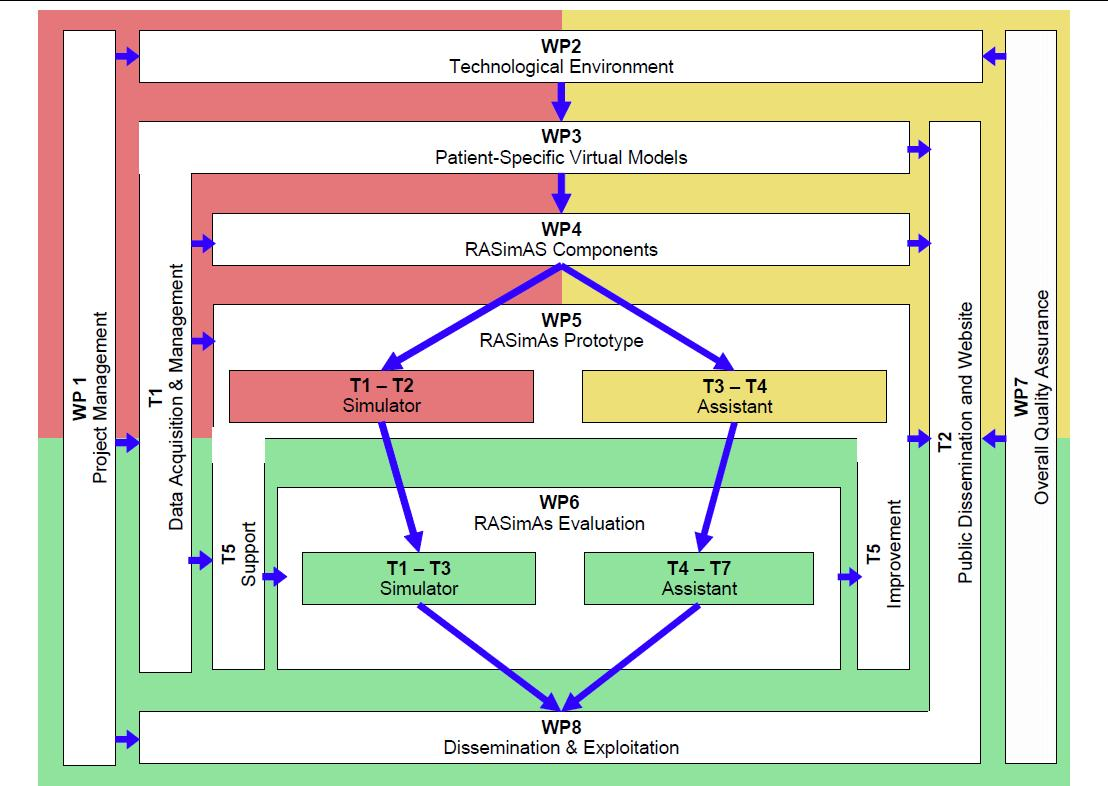
\includegraphics[width=0.95\textwidth]{IMG/wp_overview.jpg}
    \caption{División y organización de los \acl{WP} de \acs{RASimAs}.}
    \label{fig:wp_rasimas}
\end{figure}

El proyecto \ac{RASimAs} se organiza en los ocho \ac{WP} que se pueden observar en la figura \ref{fig:wp_rasimas}. Los \ac{WP} 1, 7 y 8 se encargarán de tareas de gestión: coordinación, control de calidad, diseminación de resultados y explotación de los prototipos. El \ac{WP} 2 desarrollará la plataforma donde se integrarán todos los módulos de software y datos generados de los siguientes paquetes. En los \ac{WP} 3 y 4 se desarrollarán los componentes necesarios de los dos prototipos que se integrarán en el \ac{WP} 5. Por último, el \ac{WP} 6 se encarga de la evaluación clínica tanto del prototipo de \ac{RASim} como del \ac{RAAs}. 

En la sección \ref{art:rasimas} , se introducirán los \ac{WP} 3, 4 y 5 y las tareas en las que ha contribuido de manera activa la \ac{URJC}, en las cuales se encuadra la mayor parte de la investigación realizada en esta tesis.


\subsection{Colaboración con \acl{Bangor}}
%\todo{Aaron, se que soy un pesado, pero cuando te digo que pienses cada frase me refiero a esto. El motivo por el que las colaboraciones entre miembros del proyecto van más allá de las tareas del mismo, NO es que trabajen distintas instituciones, SINO que estos proyectos permiten conocer de forma más próxima el trabajo que se está realizando en otros laboratorios }
%\todo{Para nada considero que seas pesado, al revés, el conformista soy yo...}
%
Una de las ventajas que tienen los proyectos internacionales de esta índole es que mejoran la visibilidad del trabajo realizado por los miembros del consorcio, fomentando colaboraciones entre socios más allá del ámbito del proyecto.
%
En el caso de este trabajo de tesis, \ac{RASimAs} proporcionó la oportunidad de conocer en profundidad el trabajo del  Dr. Franck P. Vidal, miembro de la \emph{School of Computer Science} de \acl{Bangor}, en el campo de la simulación de generación de imágenes médicas de rayos X en tiempo real \cite{villard2014interventional}. El Dr. Frank P. Vidal es el responsable de la librería \emph{gVirtualXRay} \cite{gVirtualXRay}.
%
A partir de esta tecnología y la herramienta de posicionamiento de pacientes, creada en el contexto del proyecto \ac{RASimAs}, se propuso desarrollar un simulador de radiología diagnóstica en el que seguir evaluando la viabilidad de los algoritmos propuestos en este trabajo.
%que utilizará los dos módulos para permitir a un usuario practicar el posicionamiento de un paciente por parte de un radiólogo.

La radiología es una especialidad de diagnóstico por imagen que utiliza la tecnología de los rayos X. Debido a la peligrosidad de una exposición prolongada a estos rayos, un simulador que permita al radiólogo entrenar de manera segura y que pudiera ser utilizado sin restricciones de tiempo, sería de gran utilidad en el campo.
Como resultado de esta colaboración, se han podido realizar dos estancias del autor de esta tesis en la \acl{Bangor}. 

%1. El proyecto Rasimas nos da la oportunidad de trabajar con miembros de la universidad de Bangor y conocer su trabajo.2. Frank School of Health Sciences y el otro School of Computer Science and Electronic Engineering3. Trabajan en radiologia (prescisa un poco dar mas detalles. Habla de sus publicaciones)4. Se plantea adpartar y extender las técnicas desarrolladas en el contexto de RaSimasç5. La colaboración se articula en dos estancias.}







\section{Motivación}
\label{intro:motivacion}
%\del{\todo{o pones citas o no haces estas aseveraciones} El uso de simuladores de realidad virtual en medicina es muy beneficioso al poder crear entornos seguros y reproducibles para los usuarios\todo{ una cita}. El auge que han tenido estos simuladores es gracias a su idoneidad para el entrenamiento y la enseñanza de los procedimientos médicos, consiguiendo una gran aceptación en todos los campos de la medicina\todo{cita}.  Aun así, la diversidad de procedimientos y la complejidad del cuerpo humano y llevar a cabo cada tipo de simulación diferente son las principales dificultades que se presentan en un futuro a corto plazo.  Los principales problemas que se han encontrado en los diferentes simuladores médicos son los siguientes:}

%\todo{ 1. tienes que hablar de la importancia de tener una libreria de pacientes 2. de la necesidad adapatarlos a la pose de operación y 3 de las aplicacioens que necesitan modificar la pose en tiempo real.  Habla de los problemas de las ténicas de posing existentes. tienes que hablar de los problemas de posing a la hora crear librerías validas para un determinado procedimiento con una poses estática o la importancia de poder cambiar la pose en el procedimiento como con los x-ray. Indicar los problemas a la hora de modificar geometrias incompletas sin descripcion de comportamiento....}
%\todo{He visto que mucho de lo que te he dicho está en los párrafos siguientes. Reestructúralo y lo vuelvo a corregir. Recuerda. Todo lo que quieres que me vuelva a leer ponlo con new.}


En el contexto de la simulación para entrenamiento médico, es importante que un profesional sanitario en formación se enfrente a la mayor cantidad de casos y  variaciones anatómicas posibles. En general, los simuladores médicos utilizan modelos anatómicos propios y específicos que no representan toda la variabilidad posible para entrenar de forma adecuada un determinado procedimiento. 
%\new{y es por ello que su utilización quedaría sesgada y resultaría complicado generalizar este aprendizaje al ámbito médico real }.
Por ello, nuevas plataformas de entrenamiento médico están incorporando datos de pacientes reales en sus simuladores \cite{Votta2013, ZHANG2017599}. Este enfoque no está exento de problemas:
\begin{enumerate}
   %\item Los datos anatómicos de los pacientes virtuales son estáticos y representan poca variabilidad.
    %\item En cada simulador se suele crear modelos anatómicos específicos y no son transferibles entre ellos.
    \item Ningún método de adquisición de imagen médica es capaz de registrar todos los tejidos de un paciente.
    \ac{US} es la técnica más barata y segura pero su rango es muy limitado, mientras que técnicas como \ac{TC} y \ac{IRM} capturan grandes porciones de tejidos, pero son costosas y/o tiene riesgos asociados. 
    Si bien es cierto que se podrían combinar datos procedentes de distintas técnicas, es poco habitual dado  los numerosos problemas que se presentan: coste, registro de imágenes, técnicas contraindicadas para algunos pacientes (por ejemplo, el \ac{TC} abdominal en embarazadas), etcétera.
    \item No es fácil obtener las propiedades mecánicas  de todos los tejidos registrados según las distintas técnicas de imagen médica utilizadas.
    \item Es habitual que las imágenes médicas se capturen con el paciente en una posición distinta a la requerida en la intervención.
    \item No siempre está disponible toda la información específica del paciente o solo se trata de una zona concreta del paciente.
\end{enumerate}
%
Por todo lo anterior, el objetivo de \ac{RASimAs} no solo es crear una base de datos de pacientes reales, sino también de pacientes virtuales en la que estén representadas el mayor número de variaciones anatómicas posibles. Estos pacientes virtuales se construirán promediando datos provenientes de pacientes reales. Puesto que no se trata de ensayar el procedimiento en un paciente real, el método, que adapte la pose de los pacientes virtuales a la requerida en el procedimiento, no tiene por qué ser precisó desde el punto de vista físico. Basta con que el resultado sea plausible, permitiendo al médico en formación entrenar de forma efectiva.
%\del{Por tanto, se hace necesario disponer de algún método que pueda capturar variaciones anatómicas, de tal manera que pueda incorporarlas al simulador que se estuviera utilizando. En este caso, en lugar de tener un modelo anatómico con una configuración concreta, % En la motivación, cuando hables de la base de datos, di que en muchas aplicaciones lo importante es la variabilidad anatómica, no trabajar con pacientes reales. }
%basta con poder transformar cualquier modelo de paciente virtual existente a una pose plausible, pudiéndose utilizar en cualquier simulador que así lo requiera. De esta forma, se intenta abarcar la mayor cantidad posible de situaciones que puedan ayudar a los aprendices a mejorar su entrenamiento y por tanto su profesionalidad .}
 
Cabe destacar que, dentro de la generación de imágenes por computador, existen diferentes técnicas para poder animar personajes virtuales.
Estas técnicas suelen estar divididas comúnmente entre métodos geométricos y métodos basados en física. Ambos enfoques presentan ventajas e inconvenientes sobre los otros y su uso dependerá de sus características. 

Considerando los problemas citados anteriormente y las restricciones impuestas por el proyecto \ac{RASimAs} (ver sección \ref{posing:req}), esta tesis pretende comprobar si es posible diseñar un método geométrico que permita reposicionar pacientes virtuales, que se utilizarán para entrenar en un entorno médico de forma efectiva. A continuación, se muestran las diferencias entre ambas aproximaciones:

\begin{itemize}
\item Los métodos basados en modelos físicos se centran en conseguir deformaciones precisas, frente a los geométricos que proporcionan soluciones plausibles. Es decir, deformaciones que el usuario pueda interpretar como reales. 
%\todo{esto es una ventaja? quizás habría que poner arriba en vez de ventajas, diferencias}
%OK


\item Los algoritmos geométricos son más robustos. En la mayoría de los casos, son soluciones \emph{ad hoc} que no sufren de los problemas de estabilidad de los métodos numéricos que se utilizan para resolver las ecuaciones diferenciales que modelan el comportamiento de los objetos físicos. %\del{ante la falta de una descripción completa de un modelo anatómico. Debido a las dificultades que tienen la adquisición de imágenes médicas, no es habitual que todas las estructuras anatómicas estén presentes o se puedan capturar el comportamiento de todas ellas.}

\item Por otro lado, los métodos físicos requieren caracterizar mecánicamente los tejidos que se van a simular. Está información no siempre puede obtenerse de forma precisa a partir de las imágenes médicas.

\item Debido a la complejidad de los comportamientos que deben simularse, la mayoría de los algoritmos biomecánicos actuales se centran en el comportamiento de estructuras concretas, como por ejemplo los sistemas de animación músculo-esquelético que obvian las interacciones con otras estructuras. 

\item Es habitual que los métodos geométricos tengan tasas de refresco altas, en comparación a los algoritmos basados en física. Habitualmente, estas técnicas son demasiado costosas para conseguir tasas de refresco interactivas. El problema se agrava cuanto más complejos sean los comportamientos que se quieran reproducir. Destacar que la simulación biomédica tiene un alto grado de complejidad debido a la variedad de estructuras y comportamientos mecánicos a simular.

\end{itemize}

Disponer de un método geométrico que permita adaptar la postura a modelos anatómicos humanos ayudará a:

\begin{itemize}
    \item Poder modificar cualquier modelo virtual con estructuras anatómicas internas a la posición requerida por un procedimiento médico.
    \item Poder adaptar cualquier paciente virtual, aunque no presente tejidos completos o cuyas propiedades mecánicas no hayan sido registradas.
%\del{El método permite una interacción inmediata y servirá para utilizarse en simuladores de entrenamiento médico????}
%\todo{Su flexibilidad y su rapidez le hacen posible incorporarlo en cualquier simulador o herramienta de \ac{RV}. REDACTA BIEN}
    \item En el contexto del entrenamiento médico, poder incorporarlo en cualquier simulador o herramienta de \ac{RV} gracias a su flexibilidad y sus tasas de refresco interactivas. 
\end{itemize}


\section{Hipótesis de partida} 
\label{intro:hipotesis}
%\todo{la hipótesis de partida es buena}
Con las motivaciones anteriormente descritas, se procede a formular la siguiente hipótesis de partida:

%\emph{es posible crear un método geométrico para animar modelos anatómicos humanos en tiempo real del que no se posean completamente todos sus tejidos o propiedades mecánicas que pueda ser utilizado en simuladores médicos para entrenar nuevos médicos. }

%\emph{ En el contexto del entrenamiento en simuladores médicos, se pueden diseñar algoritmos geométricos capaces de adaptar la antinomia del paciente virtual a la pose requerida en el procedimiento simulado de forma que la transferencia de competencias sea efectivo.}

\begin{center}
    \begin{minipage}{0.9\linewidth}
        %\vspace{5pt}%margen superior de minipage
        {
\emph{Es posible diseñar un algoritmo geométrico capaz de adaptar modelos anatómicos de un paciente virtual desde una posición inicial a la pose requerida por un procedimiento médico y que sirva para que la transferencia de competencias sea efectiva en el contexto de formación utilizando simuladores de realidad virtual. }
        }
        %\vspace{5pt}%margen inferior de la minipage
    \end{minipage}
    
    
\end{center}




% Hipótesis:
% -        Método geométrico puede ser utilizado en el contexto de los médicos:
% o   Datos incompletos (geométricos y mecánicos)
% o   Velocidad para el tiempo real. 
%o   Otras ideas
\section{Objetivos}
\label{intro:objetivos}
%\todo{Cuida más los objetivos. Mas o menos se entienden pero tienen que sonar claros y rigurosos.}
%Con la  cuando la posición del paciente en el momento que se adquiere una imagen médica (por ejemplo \ac{IRM} o \ac{TC}) es normalmente diferente a la posición requerida por el procedimiento médico que se este simulando. A la vez, estas imágenes suelen ser locales y no son capaces de recuperar cada uno de los tejidos del paciente o su comportamiento mecánico.

Con la hipótesis de partida enunciada, a continuación, se presentan los objetivos principales que se pretenden alcanzar a lo largo de la presente tesis:

%\todo{Asegurar que todo esta escrito en futuro}
\begin{itemize}
\item Diseño de un algoritmo para el posicionamiento de modelos anatómicos, desde la posición en la que fueron modelados hasta cualquier posición requerida.
\\
%\todo{no puede ir en pasado son objetivos!!!!. Escríbelos como tales}

Se propondrá una técnica que permita transformar los modelos anatómicos de pacientes virtuales, los cuales originalmente se encuentran en una postura diferente a la posición necesaria para el entrenamiento de un determinado procedimiento médico. %\todo{desde la coma suana raro}. 
La técnica propuesta será capaz de modificar un modelo anatómico con estructuras internas de manera interactiva, siendo esto posible, aunque el modelo no fuera completo o no estuvieran disponibles las propiedades mecánicas de los tejidos. En resumen, la técnica que se proponga deberá verificar los siguientes requisitos:
%\todo{sin necesidad de disponer de una descripción mecánica de las porpiedades de los tejidos y incluso sin disponer de un modelo completo, es decir, no es necesario que estén modeladas todas las estructuras anatómicas. (Pon esto bonito)}

\begin{itemize}
%\todo{Yo aquí subdividirá el objetivo 1 en los requisitos de la técnica}
    \item Debe funcionar en tasas interactivas.
    \item Debe poder trabajar con modelos incompletos.
    \item No necesita las descripciones mecánicas de los tejidos.
    
\end{itemize}

%\todo{Tenemos que hablar.  2. La idea es probar el algortimo en dos casos de uso reales. Uno que demuestre que funciona con información incompleta y otro que demuestre que funciona en aplicaciones interactivas. Ojo con decir que probamos que la transferencia de conocimientos es adecuada, no lo hacemos!!!!. Tienes que insinuarlo sin dejarlo explicito.

\item 	Validación del algoritmo. \\

%\todo{Yo diría en los objetivos que la técnica servirá para entrenar si se al incorporarla en simuladores estos pueden usarse para entrenar.}
%\todo{Los objetivos son muy importantes. Redacta esto mejor. }
Con el fin de demostrar que el algoritmo propuesto puede ser utilizado en el entrenamiento médico, este será incorporado en dos tipos de aplicaciones de \ac{RV}. En el primer caso, se intentará demostrar que el algoritmo puede adaptar la postura de un modelo anatómico en un escenario donde no se disponen de modelos completos desde un punto de vista anatómico y de los que tampoco se dispongan los parámetros que caracterizan el comportamiento mecánico de las estructuras presentes. En el segundo caso de uso, el algoritmo mostrará su utilidad en un entorno donde el usuario deberá modificar interactivamente la posición del paciente como parte del procedimiento. 

%Objetivos secunadrios:

%- Objetivos del algoritmo

%- Objetivos de los dos casos de uso.

%--- Recureda. En el simuladador de anestesia regional no se cambia la pose en tiempo real (validamos descripciones incompletas)

%--- El de radiología la selección de la pose es parte del comportamiento, aunque por otro lado hay menos estructuras anatomicas relevantes.

\begin{itemize}
    \item 	Caso de uso: Simulador de anestesia regional y herramienta \acs{ITGVPH} 
    %\todo{No me gusta que lo vendas como offline. Hemos vendio que un experto valida la pose por lo que la herramienta itne que ser interactiva.}:
    
    Un objetivo del proyecto \ac{RASimAs} es la creación de la herramienta \ac{ITGVPH} para generar una base de datos con pacientes virtuales que representen distintas variaciones anatómicas promedio y que posteriormente será utilizada en \ac{RASim}.
    El algoritmo propuesto se integrará y comunicará con otros módulos que componen la herramienta, permitiendo animar y adaptar los \ac{VPH} generados. El método estará en comunicación con otros módulos desarrollados dentro del proyecto \ac{RASimAs}. Además, se desarrollarán los módulos del simulador con la finalidad de comprobar si la generación de estos \ac{VPH} es útil para entrenar el procedimiento de \ac{RA}.
    
   % \del{Además, se desarrollará un \emph{software} (\acs{Courseware}) para el simulador \ac{RASim} que se encargará de la comunicación con los demás módulos, y gestionará la interacción del usuario en una plataforma de entrenamiento auto guiada.}\todo{El courseware no es un objetivo. Lo que haces es desarrollar modulos del simulador de cara que este pueda utilizarse para entrenar a pacientes. No des muchos más detalles.} 

%\todo{Idea, no se necesitan pacientes reales sino pacientes medios. No se necesita una deformación presica, sino plausible}

%\todo{No entiendo este segundo parrafo. Puedes hablar del curseware. No se porque hablas de los hapticos y del Hw eso va antes?????}
    

    \item Caso de uso: Simulador de radiología diagnóstica

%\todo{Lo que tienes que vender aquí es que el posing del paciente es parte integral del procedimeinto y que se requiere un algorimo robusto que funcione en con tasas de refresco interactivas.}
%En este caso de uso, el algoritmo propuesto permite al usuario modificar la postura del paciente con el objetivo de entrenar el procedimiento de radiología diagnóstica.\todo{no has dicho nada} 
En radiología diagnóstica, el médico debe posicionar al paciente y configurar la máquina de rayos X de manera que la región anatómica objeto de estudio sea adecuadamente capturada. El algoritmo propuesto permite modificar la posición de un paciente virtual interactivamente, permitiendo probar distintas proyecciones y obtener imágenes de rayos X simultáneamente. El simulador permitirá entrenar las proyecciones radiográficas sin ningún riesgo para el paciente o el usuario. Este simulador, podrá ser usado tanto por profesores como por estudiantes de radiología como una herramienta adicional a las técnicas clásicas de aprendizaje.
\end{itemize}

\end{itemize}

% \begin{itemize}
%     \item 	Diseño del entrenamiento y evaluación del simulador.
% \end{itemize}

% La \ac{RV} proporciona una herramienta muy útil para poder guiar y ayudar en el proceso de aprendizaje al usuario. Mediante tareas guiadas, el usuario podrá aprender y perfeccionar el procedimiento quirúrgico, que ayudará a suavizar así la curva de aprendizaje y reducir posibles riesgos en el futuro. El simulador permitirá empezar por los caso más sencillos e ir facilitando el entrenamiento de casos más complejos. El objetivo es, que el usuario aprenda desde las competencias más básicas hasta simulaciones de situaciones reales, intentando minimizar el tiempo de aprendizaje. El usuario puede repetir el entrenamiento hasta que adquiera las habilidades requeridas. Debido a que cada vez más están presentes los simuladores en el currículum de los estudiantes de medicina, es necesario  crear unas métricas que sean útiles para evaluar a los estudiantes de manera cualitativa.




\section{Contribuciones}
\label{intro:contribuciones}

La principal contribución de esta tesis es la presentación de un algoritmo geométrico que permite modificar un modelo de paciente virtual de una postura original a la posición requerida por cualquier simulador. Este algoritmo ha sido diseñado, creando y adaptando técnicas establecidas en el cauce clásico de la animación esqueletal, pero permite animar tanto los modelos superficiales clásicos como los tejidos internos del modelo de un paciente virtual.

El algoritmo propuesto es capaz de solucionar dos grandes problemas que un usuario se puede encontrar al animar anatomía humana. Por una parte, esta técnica es capaz de manejar datos incompletos, tanto por la imposibilidad de capturar todos los tejidos dentro de la anatomía, %\todo{parece que hay gente que va por ahí sin pulmones} 
como por la falta de una descripción mecánica de los tejidos a animar. Esta característica ayuda a resolver casos donde los modelos procedentes de imágenes médicas %\ac{parciales}\todo{lo de locales no está suficientemente justificado}
no contengan la descripción del paciente al completo. Por otra parte, esta técnica permite animaciones en tiempo real para que sea posible incorporarlo en cualquier simulador. El algoritmo es lo suficientemente rápido para mover la anatomía de un modelo de cuerpo entero permitiendo tasas interactivas al usuario.

Con el objetivo de demostrar la utilidad de la técnica propuesta, se ha procedido a incorporarla en dos simuladores médicos como ejemplos de casos de uso. 

\subsection{Contribuciones a RASimAS}

%\todo{Creo que le falta peso al curseware. YO DARIA PESO AL COURSEWARE AQUÍ NO EN LOS OBJETIVOS. LO MISMO EN EL SIMULADOR DE RAYOS X}
%es una de las motivaciones\todo{así suena raro} y parte financiadora de esta tesis,\todo{dos frases} el algoritmo propuesto es una parte importante dentro de la consecución del simulador que representa uno de los dos pilares del proyecto europeo.  

%\del{ \ac{TPTVPH} donde se encuentra varios procesos, desde el registro de los datos del paciente pasando por el proceso de completar los tejidos, la definición de las propiedades mecánicas para poder crear el \ac{VPH} y por último, el posicionamiento del modelo a la postura requerida para cada procedimiento.}\todo{falso el TPTVPH es nuestra herramienta}

La participación en el proyecto \ac{RASimAs} es el punto de partida del desarrollo de esta tesis. Se ha contribuido con la creación de un algoritmo que permite la adaptación de un \ac{VPH}, de una postura inicial a una final, de manera automática o supervisada por un experto.
El algoritmo propuesto ha sido integrado dentro del entorno \ac{ITGVPH}.
Esta herramienta proporciona los modelos que se van a utilizar en \ac{RASim}, permitiendo un entrenamiento del procedimiento de \ac{RA} con una base de datos de pacientes que disponga de una amplia variabilidad anatómica.

Por otra parte, también se ha contribuido en la creación del módulo \ac{Courseware}, que gestiona todos los componentes del simulador y se encarga de implementar todas las tareas de relacionadas con el entrenamiento. \ac{RASim} se compone de varios módulos software:
\begin{enumerate}
    \item El módulo de ultrasonidos \cite{Law2015} encargado de simular el proceso de generación de la imagen de \ac{US} que se usa para guiar la aguja a su objetivo.
    \item El módulo de la simulación física que se ha implementado extendiendo la funcionalidad de la librería \ac{SOFA} \cite{sofaweb} y que se encarga de modelar el comportamiento de la aguja con \cite{needleinsertion}, de sus interacciones con los tejidos del paciente y de dar una respuesta háptica.
    \item \emph{H3D} \cite{sensegraphics2012open} es el módulo encargado de la visualización de la escena virtual y la comunicación de los dispositivos.
    \item El \ac{Courseware}, que proporciona una plataforma de aprendizaje donde el usuario podrá practicar y desarrollar sus habilidades no cognitivas.
\end{enumerate}
%\new{(i) ; (ii) ; y del (iii) .}    
Desde la \ac{URJC} se ha liderado el proceso de integración del \ac{Courseware} en el simulador, debido a que es necesaria una continua comunicación entre los módulos anteriormente citados y la plataforma de entrenamiento. El \ac{Courseware} gestionará los distintos módulos citados con la finalidad de permitir un entrenamiento autónomo y de proporcionar retroalimentación formativa y sumativa, gracias a las métricas recogidas a través de estos módulos.

En las últimas etapas del proyecto, el comité médico del proyecto no valoró positivamente la correspondencia entre dispositivos de entrada, no siendo posible su evaluación clínica. Debido a problemas de precisión de los dispositivos hápticos (presentaban defectos de fábrica), los médicos consideraron que podría introducir sesgos en los aprendices. A partir de una propuesta de la \ac{URJC}, se procedió a sustituir los dispositivos hápticos por unos \acs{tracker}s magnéticos que permitió conseguir una evaluación favorable por parte de los evaluadores.


% \todo{Explicar que:
% 1. El grupo de la URJC a liderado el proceso de integración.
% 2. Qué la plataforma haptica no contó on el visto bueno de los medicos implicados en proyecto. (Explica los problemas)
% 3. Indica que como parte de está tesis sutituiste el modulo haptico por un sistema basado en tracker magenticos que si conto con la aprobación de los medicos. }


\subsection{Simulador de radiología diagnóstica}
%El algoritmo presentado en esta tesis permite ser incorporado en cualquier simulador que requiera transformar la postura de un modelo anatómico con estructuras internas interactivamente.
%\todo{es muy repetitivo}
Como resultado de la colaboración con el Dr. Franck P. Vidal, se ha desarrollado un simulador de radiología diagnóstica con la librería \emph{gVirtualXray} \cite{sujar:hal} y el algoritmo propuesto. Esta herramienta interactiva permite practicar las proyecciones radiológicas de manera segura y sin necesidad de pacientes reales.  El simulador podrá ser usado tanto por los profesores como por los estudiantes de radiología, complementando así el material utilizado en clase. Con el objetivo de practicar con una amplia variabilidad anatómica, el algoritmo propuesto ofrece la posibilidad de incorporar modelos de pacientes virtuales creados externamente. Para ello, cuenta con un preproceso que permite preparar los pacientes virtuales para el algoritmo teniendo unos requisitos mínimos. Esta etapa se ejecuta de manera automática y solo se ejecuta una vez por modelo.

%\todo{Indica que gracias a la flexibilidad del algoritmo de posing se han integrado distintos modelos creados por terceros y que el simulador permite la incorporación de nuevos modelos con un numero de restricciones mínimas, aplicando un pre-proceso en su mayor parte automatico.}



%\todo{intenta acortar la frase.}
Al igual que \ac{RASim}, se ha desarrollado un \ac{Courseware} que permite al usuario practicar el procedimiento de forma guiada y autónoma a la vez que permite al profesor diseñar ejercicios de clase. Finalmente, se realizó un estudio para validar su utilidad en el que 18 participantes realizaron una encuesta donde se les enseñaba las distintas funcionalidades del simulador y se les preguntaba acerca de su opinión. Los resultados obtenidos sugieren que el simulador es lo suficientemente realista para que sea útil como herramienta de enseñanza y entrenamiento del procedimiento.
%\todo{Yo también explicaría que el simulador esta pensado como herramienta de clase puesto que su uso como entranador 

%\todo{Si conseguimos la validación la ponemos aquí}
%\todo{requeriria una validación que va más allá del ambito de esta tesis aunque la funcionalidad de entrenamiento ha sido implementada. Aaron: Al final no he validado nada entonces? Quizás sea mejor no ponerlo aquí}
%\todo{Explica un poco el curseware y/o los modos de funcionamiento...}


%cuales son mis contribuciones al simulador y que módulos han sido cogidos 

\clearpage
\section{Estructura de la tesis}

Después de este capítulo de introducción, el resto del documento se organizará de la siguiente manera:

En primer lugar, se introducirá en el capítulo \ref{cap:related} la bibliografía necesaria para poner en contexto al lector. Se presentará información relativa a:
\begin{itemize}
    \item Formación de profesionales médicos.
    \item Caracterización de los procedimientos presentes en esta tesis.
    \item Organización del proyecto \acs{RASimAs}.
    \item Revisión bibliográfica sobre las técnicas geométricas y basadas en modelos físicos de la animación de personajes.
\end{itemize}

A continuación, en el capítulo \ref{cap:posing}, se presentará el algoritmo de posicionamiento de pacientes virtuales, el cual es la principal contribución de esta tesis, y los trabajos realizados para la consecución de los objetivos de la tesis. En los siguientes capítulos, se presentarán los casos de uso donde se ha integrado el algoritmo propuesto para demostrar su utilidad. En el capítulo \ref{cap:rasim}, se detallará la integración del algoritmo en la herramienta \acs{ITGVPH} y el desarrollo del módulo \acs{Courseware} en el simulador \acs{RASim}. En el capítulo \ref{cap:xray}, se presentará el desarrollo del simulador de radiología diagnóstica donde se integró el algoritmo propuesto junto con la librería \emph{gVirtualXRay}.

En el capítulo \ref{cap:results}, se exponen los resultados obtenidos por el algoritmo de posicionamiento de pacientes virtuales en cuanto a calidad y rendimiento. Además, se presentarán los problemas ocurridos dentro del proyecto \ac{RASimAs}. Al final, se mostrarán los resultados del simulador de radiología diagnóstica junto con las  validaciones de apariencia y de contenido realizadas. 

Finalmente, en el capítulo \ref{cap:conclu} se resumirán las conclusiones y contribuciones de la presente tesis. Por último, se podrán consultar los apéndices y la bibliografía utilizada.

%%%% Antecedentes
\chapter{Antecedentes} 

\label{cap:related}
%\todo{
% Hay varias cosas en relación a la estructura de este punto que debes mejorar.
% Te planteo primero los problemas y luego una posible solcuicón:
% 1. No entiendo porque hablas de las la RA y de la radiolaogia diagnostica en le punto 1.1. 
% 2. No entiendo porque el punto 1.1.1 y el 1.3 están separados. 

%Solución 
%1.1 Simuladores Médicos de Realidad Virtual
%1.1.1 Técnicas tradicionales (sin hablar de simuladores RV, lo que tengas pasaló al actual 1.1.3 )
%1.1.2 Simuladores RV (Aquí va todo lo de G. Burdea)
%1.1.3 Simuladores médicos (fusión de los actuales 1.1.1 y 1.3) cuando los fusiones que no te quede muy repetitivo. Vuelvelo a leer.
%1.1.3.1 Aprendizaje (no me gusta mucho el título)
%1.1.3.1 Evaluación. Mete validez dentro
%1.2 Caracterización de los procedimientos simulados
%1.2.1 RA
%1.2.3 x-ray (los titulos antiguos)
%1.3 RASimAs
%1.4 Como está
%}


En este capítulo se repasará la bibliografía con el objetivo del ayudar al lector a entender mejor el alcance de esta tesis.
Además, se explicará en detalle la estructura del proyecto \ac{RASimAs}, haciendo especial hincapié en las partes desarrolladas en este trabajo. El lector también podrá encontrar una revisión bibliográfica en la que se repasan los principales avances que se han producido en los últimos años en el área en la que se enmarca esta tesis, destacando sus fortalezas y debilidades. 

Se va a comenzar dando una perspectiva general de los simuladores de realidad virtual para luego centrarse en simuladores particulares de especial relevancia para el contexto de esta tesis. A continuación, se introducirán brevemente conceptos relacionados con el aprendizaje en este tipo de plataformas. También se detallará la evaluación a la que se someten los simuladores de realidad virtual, en concreto en el ámbito médico, para probar su efectividad. Posteriormente, se presentarán al lector los procedimientos médicos en los que se ha trabajado en esta tesis. Además, se resumirá la división de tareas del proyecto \ac{RASimAs}. 
Finalmente, se introducirá al lector en el estado del arte en la animación de personajes dentro de la informática gráfica, haciendo hincapié en aquellas técnicas relacionadas con el método propuesto en este proyecto. Esta sección se centrará en describir las etapas de la animación esqueletal en las que está basado el algoritmo propuesto en esta tesis y las distintas alternativas que existen para automatizarlas y, por último, se compararán con los métodos de animación basados en modelos físicos.



\section{Simuladores para formación médica}
\label{art:medicalsim}

En los últimos años, los simuladores médicos de realidad virtual están tomando una gran importancia en el currículum de los estudiantes, tanto en el campo de la cirugía como en el de otras especialidades \cite{PATEL2017266.e7}. Se puede observar un incremento de su presencia para el entrenamiento de jóvenes especialistas tanto en hospitales como universidades. Estas herramientas proporcionan al usuario un método seguro y efectivo de entrenamiento \cite{simsafety}.

\subsection{Técnicas tradicionales}

Aunque los simuladores están cobrando cada vez más importancia en el ámbito médico, la enseñanza actual se apoya en una gran variedad de métodos de entrenamiento, que permiten al médico adquirir las destrezas necesarias, antes de poder enfrentarse a escenarios reales de manera autónoma. 

%\todo{aprendizaje teórico  usanado libros de texto y bases de datos de casos clínicos.(destrezas cognitivas)
%Especialmente en radiologia.  No permiten la adquisición de destrezas no-cognitivas al no permitir interactuar con el paciente.}

El principal método clásico es el aprendizaje teórico, utilizando los libros de texto y la lectura de casos clínicos archivados. 
De esta manera, los profesionales adquieren las destrezas cognitivas necesarias. Aun así, con este método no es posible la adquisición de aquellas habilidades no-cognitivas debido a la ausencia de interacción o práctica que simule un escenario real. 
Para suplir la falta de estas destrezas, la forma de entrenamiento más habitual era la práctica supervisada sobre pacientes reales (\emph{by doing}), donde el estudiante realizaba el procedimiento vigilado y guiado por su tutor. Aunque es el entrenamiento más realista, desde hace décadas se intenta limitar su uso debido a que viene acompañado de situaciones no controladas y de riesgos para el paciente. % \todo{desde la coma suena raro}

Una forma segura de entrenamiento es la utilización de \emph{fantomas}\footnote{Castellanización del término inglés Phantom} \cite{phantomra}. 
Los \emph{fantomas} son modelos anatómicos hechos con materiales sintéticos que intentan replicar el cuerpo humano y sus propiedades de la forma más fiel posible. En la figura \ref{fig:phantom} se puede ver un ejemplo diseñado para la práctica de ultrasonografía, el \emph{Blue Phantom™} \cite{BluePH}. En ocasiones, estos maniquíes tienen incorporados una serie de sensores que permiten la recogida de métricas de rendimiento. Pero a pesar de que son muy populares, tienen una serie de inconvenientes. Por ejemplo, no son baratos y se crean específicamente para una zona anatómica concreta. No es posible usarlos con otro fin que entrenar el procedimiento para el que fueron diseñados. Además, en determinadas ocasiones, como puede ser hacer una incisión o realizar una inyección en el \emph{fantoma}, el usuario tiene que manipularlos, lo que se traducirá en desgaste con el tiempo. Por último, destacar que estos modelos representan una única variedad anatómica, haciendo que el médico se enfrente al mismo escenario una y otra vez.
\begin{figure}[ht]
   \centering
    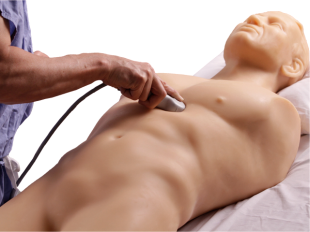
\includegraphics[width=0.8\textwidth]{IMG/fast_trauma.jpg}
    \caption{Maniquí realista para el entrenamiento de ultrasonografía  \emph{Blue Phantom™} \cite{BluePH}. }
   \label{fig:phantom}
\end{figure}

Otra forma de entrenamiento es la utilización de cadáveres \cite{Tsui2007}. De esta manera, el médico puede enfrentarse a casos reales. En este caso, conseguir diferentes variaciones anatómicas es completamente viable y el mismo cadáver puede servir para entrenamientos de diferentes procedimientos. Aun así, los inconvenientes que presentan son bastante evidentes. 
%\todo{Rehaz la última frase. También indicar que la disponibilidad de cadáveres es baja y que no se puede repetir el entrenamiento sobre el mismo paciente. }
La baja disponibilidad de cadáveres y su dificultad para mantenerlos en buenas condiciones, representan sus principales problemas. En ocasiones, los motivos del fallecimiento pueden perjudicar al estado del mismo, o no es posible repetir el mismo entrenamiento en el mismo cuerpo en más de una ocasión. Incluso, existen problemas éticos si se pretenden utilizar cadáveres procedentes de condenados a pena de muerte (Visible Human Project \cite{ackerman1998visible}).
Finalmente, uno de los grandes inconveniente de la utilización de cadáveres es que sus tejidos no muestran el mismo comportamiento mecánico que un tejido vivo. Esto puede inducir s sesgos en el entrenamiento del profesional médico, debido a que los músculos se vuelven más rígidos después del fallecimiento (efecto conocido como \emph{rigor mortis}).

\subsection{Simuladores de realidad virtual}
\label{art:simulador}

\begin{figure}[ht]
   \centering
    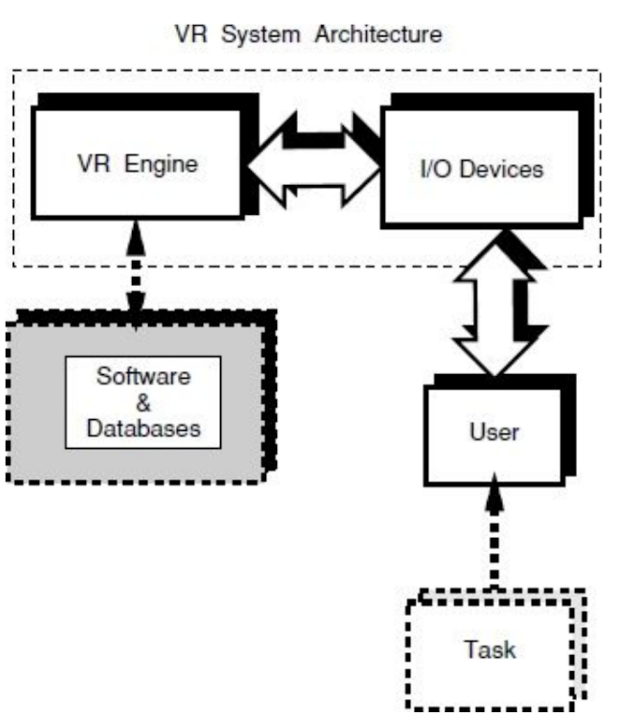
\includegraphics[width=0.5\textwidth]{IMG/VRarq.PNG}
    \caption{Arquitectura para sistemas de \acs{RV} propuesta por \emph{Burdea y Coiffet} \cite{burdea2003virtual}. }
   \label{fig:RVarq}
\end{figure}

%\todo{He metido cambios en la intro y en la sección 1.1 sin el control de cambios. Creo que es peligroso (aunque son muy pequeños). A partir de ahora resaltaré toda la frase aunque el cambio sea mínimo.}
Antes de continuar con la revisión bibliográfica de los simuladores para entrenamiento médico, se van a introducir los conceptos básicos que definen la arquitectura de un sistema de \ac{RV}. %\del{Esto es importante para entender la diferencia que hay entre un simulador de \ac{RV} frente a un simple computador. En esta sección se presenta una propuesta de arquitectura para simuladores de realidad virtual. Esta arquitectura puede ayudar al lector a hacerse una idea de cómo se han construido los simuladores que se presentarán en las siguientes secciones. Además, se utilizará en el capítulo \ref{cap:rasim} como apoyo para explicar el simulador \ac{RASim} y sus diferentes componentes. }
Según \emph{Burdea y Coiffet}\cite{burdea2003virtual}, un sistema de \ac{RV} se puede dividir en cinco componentes tal y como se puede observar en la figura \ref{fig:RVarq}. En ella, además, se puede observar las distintas interacciones que se producen entre estos componentes. Es la relación que existe entre ellos, la que conforma un sistema de \ac{RV}. A continuación, se describirán cada uno de ellos:
\begin{itemize}
    \item Motor de \ac{RV}: este componente se encarga de realizar los cálculos necesarios para simular la escena virtual. Para actualizar el estado de la escena virtual es necesario que se consulten las bases de datos y actuar según la interacción de los usuario a través de los dispositivos de entrada. El motor generará y mostrará el nuevo estado de la escena a través de los dispositivos de salida (que pueden incluir más de un canal sensorial). Además, es preciso asegurar una tasa de refresco interactiva. El término motor de \ac{RV} no se puede asociar a un computador, sino que se tiene que tratar como una abstracción ya que puede tener múltiples configuraciones hardware, como puede ser un único computador o un sistema distribuido conectado por red.
    \item Dispositivos de \ac{E/S}: este componente lo forman todos los dispositivos que utiliza el usuario en su interacción con el sistema. Es imprescindible para un sistema de \ac{RV}  que se permita la interacción del usuario. Los dispositivos de entrada se encargan de recoger las acciones que realiza el usuario, mientras que los dispositivos de salida muestran la respuesta de la escena virtual a través de los distintos canales sensoriales. Actualmente, estos dispositivos son muy numerosos y diversos.
    \item Componentes software y base de datos: este módulo contiene todas las especificaciones y descripciones que caracterizan el software del sistema. Por una parte, análogamente a una base de datos tradicional, donde se consulta y se recoge información, el resto de módulos consultarán la escena para ejecutar simulación.
    Por otra parte, también es importante nombrar aquellas aplicaciones que se diseñan con el objetivo de guiar y facilitar el entrenamiento. Estas aplicaciones definen como será la interacción del sistema y el usuario a través de la simulación y dan al usuario un motivo para interaccionar con el sistema.%\todo{Rehaz la última frase.}
    \item Usuario: el principal objetivo de la \ac{RV} es presentar al usuario una escena virtual que este perciba como una representación plausible de la realidad. En este sentido, el usuario y la forma en que este percibe e interactúa con el mundo es clave a la hora de diseñar cualquier aplicación \ac{RV}.
    %\del{Es natural que los sistemas se diseñen con el objetivo de que una persona interaccione con ellos. Esta comunicación se realizará a través de los dispositivos de \ac{E/S}}. 
    \item Tareas: por último, son las tareas, objetivos e instrucciones que recibe el usuario cuando va a utilizar el sistema de \ac{RV}, las que dan significado y utilidad a la aplicación. Es lo que diferencia un computador con periféricos conectados de una plataforma de \ac{RV}.
\end{itemize}


%%%%%%%%% CAMBIO DE SECCION

\subsection{Entrenamiento con simuladores médicos}
\label{art:entrenamiento}


%En anteriores secciones se ha revisado el uso de simuladores en medicina aunque es bien sabido que el uso en otro tipo de contextos no es nuevo. El principal objetivo de estos simuladores es garantizar la seguridad e intentar mejorar el aprendizaje y la respuesta antes errores poco comunes.

En \cite{donaldson2000err}, se cifra en cientos de miles las muertes ocurridas en hospitales estadounidenses como consecuencia de errores médicos, eso sin contar otros tipos de daños a los pacientes que implican gastos económicos. En este libro se planteaba la necesidad de mejorar la formación de los profesionales para evitar este tipo de errores. 
Es necesario también garantizar la seguridad y la intimidad de los pacientes durante el proceso de aprendizaje, lo cual lleva implícito la exigencia ética que representa el propio código deontológico del personal sanitario. 

En el libro \cite{dent2017practical}, se presentan una serie de objetivos que debería cumplir una institución de enseñanza médica al formular el currículum del personal sanitario.
\begin{itemize}
    \item Producir nuevos profesionales sanitarios.
    \item Utilizar los procedimientos médicos modernos.
    \item Cumplir la regulación gubernamental.
    \item Asegurar que los estudiantes puedan completar el curso.
    \item Satisfacer las expectativas de los pacientes.
\end{itemize}

Estos objetivos se enfrentan con una serie de problemas que han impulsado a las instituciones médicas a potenciar el uso de los simuladores.
Por una parte, desde hace décadas se viene disminuyendo el tiempo de trabajo para los profesionales en formación, lo que se traduce en la reducción del tiempo con pacientes reales. Además, ha habido cambios respecto a que un paciente sea objeto de exploraciones y procedimientos redundantes, con la finalidad de entrenar a estudiantes, siendo esta práctica una molestia y un peligro para el paciente. También, hay que añadir que diversos movimientos por los derechos de los animales han hecho restringir el uso de estos con motivos de entrenamiento. Por otra parte, ciertas organizaciones han cambiado sus métodos de evaluaciones con acreditaciones y certificaciones frente a la clásica evaluación basada en el conocimiento exclusivamente.

Otro motivo por el cual es necesario cambiar las formas de aprendizaje de la medicina, es que estas también han evolucionado con el tiempo.
Tradicionalmente, el plan de estudios de la medicina era incremental, desde los aspectos más básicos hasta llegar a la especialización. Actualmente la medicina es tan extensa que el contenido del currículum se ha incrementado notablemente. Esto ha hecho que aparezcan escuelas para cada especialidad médica donde el conocimiento ha crecido exponencialmente en las últimas décadas y los métodos tradicionales de enseñanza no están completamente adecuados para manejar esa cantidad de material.

Obligados a buscar alternativas para garantizar una exposición clínica variada y completa, junto con el desarrollo de la investigación en el campo de la simulación, los simuladores de \ac{RV} están aumentando su presencia dentro de los procesos de aprendizaje de los futuros médicos.

Frente a un modelo asistencial en la formación de los estudiantes, los simuladores presentan  ventajas educativas que convierten estas herramientas en ideales para enfrentarse a los problemas anteriormente citados. Estas herramientas han demostrado que pueden reducir el tiempo de realización de una tarea, así como el número de errores cometidos y, además, siendo posible diferenciar entre expertos y novatos \cite{Gurusamy08}.

Por otra parte, los simuladores permiten que el estudiante cometa errores sin consecuencias reales. %sin las consecuencias reales que podrían resultar en un entorno con pacientes.
El alumno se puede enfrentar a todo tipo de situaciones, desde las introductorias a las más complicadas donde errar no es crítico. Citando a \cite{ziv2008educacion}: "Los errores son experiencias de aprendizaje y ofrecen grandes oportunidades de mejorar a través del aprendizaje de los mismos". Además, permite que el alumno reciba valoraciones y comentarios en tiempo real. Los simuladores presentan un entorno educativo estandarizado, reproducible y objetivo que permite una evaluación constante de los estudiantes.

A diferencia de los métodos tradicionales anteriormente citados, los simuladores de realidad virtual permiten un entrenamiento más barato y rápido donde los estudiantes pueden mejorar sus habilidades, especialmente las no cognitivas. Mejoras en el rendimiento, nuevos dispositivos de \ac{E/S} y el desarrollo de nuevas técnicas de simulación física, permiten una transferencia efectiva de habilidades del mundo virtual al mundo real \cite{dawereview}.
Habitualmente los simuladores son específicos de cada procedimiento médico, como por ejemplo en \cite{cecil2017advanced} donde se presenta un simulador de cirugía ortopédica. Es también muy habitual encontrar simuladores de cirugía cardiovascular como \cite{korzeniowski2018vcsim3}. En algunos casos se combinan tecnologías de dos o más especialidades para realizar un procedimiento concreto. En  \cite{villard2014interventional} se presenta un simulador de radiología intervencional donde se entrena la habilidad quirúrgica a la vez que se practica el guiado de la aguja a través de una imagen de rayos X.

Pero además, la nueva generación de simuladores no solo se centra en mejorar las habilidades no-cognitivas. Los simuladores permiten entrenar con una gran variabilidad anatómica, desde ejemplos de casos simples hasta los más complejos. Existe la tendencia de permitir el entrenamiento de procedimientos incorporando datos de pacientes, que proporcionen ejemplos reales que se puedan encontrar en un futuro \cite{Willaert2012, ZHANG2017599}. 
%\todo{Esta idea queda huérfana aquí. Tienes que desarrollarla. }

El ámbito de los simuladores médicos es muy amplio por lo que, a continuación, la revisión bibliográfica se centrará en las dos especialidades que se van a tratar en la presente tesis.


En cuanto a la especialidad de anestesiología, la anestesia espinal y la epidural son los dos ejemplos más frecuentes dentro de la \ac{RA}, en los cuales se pueden encontrar simuladores específicos, como por ejemplo \cite{broom2018evaluation}. %Sin embargo, la búsqueda de un simulador de \ac{RA} genérico es más complicada.

En cuanto a la existencia de simuladores de \ac{RA} genéricos, se pueden encontrar algunos ejemplos en la bibliografía. Por ejemplo, \emph{Energid Technologies} ha desarrollado un simulador al amparo de un contrato con el Ejército de Estados Unidos, sin embargo, el producto final no se ha comercializado al público \cite{lim2008simulation}. Al contrario, un simulador comercial llamado \emph{SAILOR}, se distribuye acompañado de un atlas multimedia de los bloqueos de nervios. Este simulador presenta solo un único modelo de paciente, y su interacción es exclusivamente con el ratón sin ningún tipo de deformación del tejido \cite{Bibin}. 

En un estudio previo al proyecto \ac{RASimAs}, se demostró la aceptación que tendría un simulador para la \ac{RA}. Todos los participantes se mostraron muy receptivos con el trabajo realizado pero se recalcó la escasez de nervios para bloquear, la pobre simulación de los ultrasonidos y la ausencia de respuesta háptica \cite{Grottke2009594}.


%\todo{mirar lo que añadió graham}
En cuanto a la enseñanza de radiología diagnóstica, la forma más común de aprender diagnóstico por imagen son los archivos educativos, que son recopilaciones de imágenes médicas de pacientes reales acompañados del historial del paciente. En estos archivos, los estudiantes pueden buscar a través de la gran cantidad de casos bien documentados. Es habitual que cada universidad, hospital o facultad, tengan sus propios repositorios. Además, existen libros donde se pueden consultar recomendaciones y guías \cite{carver2012medical,manualpractico}. 
En la última década, estos recursos se publican cada vez más de manera \emph{online}, donde cualquier radiólogo pueda consultar una enorme base de datos de imágenes de cualquier parte de la anatomía humana \cite{deshpande2017integrated}. 


Actualmente, la educación se ha visto beneficiada por la incorporación de los teléfonos inteligentes. Esto ha provocado que algunas instituciones hayan creado aplicaciones mediante las cuales los estudiantes pueden revisar e investigar los casos almacenados, realizar cuestionarios y mejorar el aprendizaje como es el caso de la aplicación \emph{UBC Radiology} \cite{Spouge2017}. %Estos recursos se encuentran muy presentes en el aprendizaje de los radiólogos noveles.

Complementando la formación teórica, es habitual que se utilicen \emph{fantomas} para entender los principios básicos de radiación sin riesgo de dañar un tejido orgánico. Como se ha comentado anteriormente, estos modelos anatómicos son muy caros y no es posible disponer de la cantidad necesaria para representar una gran variabilidad anatómica.

Tanto estos recursos como los archivos educativos mantienen el mismo problema: las imágenes registradas son estáticas, y la mayoría de ellas corresponden a imágenes que se presuponen son correctas y no muestran ningún tipo de fallo. Esto es completamente entendible, ya que al hacer este tipo de recursos se seleccionan aquellas imágenes que no inducen a error al estudiante. Además, en estos recursos, rara vez aparece un paciente en más de una pose o no es posible ver la misma anatomía u otras partes del mismo sujeto que puedan mostrar diferentes situaciones al estudiante. Aun así, posicionar bien al paciente mientras se realiza el diagnóstico por imagen es imprescindible y necesario que el estudiante domine. 


Por otra parte, las mejoras en el rendimiento de los computadores permiten crear nuevos simuladores que mejoran y reducen el tiempo de aprendizaje de los estudiantes. Un caso notable es el  ProjectionVR$^{TM}$ \cite{shanahan2016student}. Este simulador trata de introducir al usuario dentro de un entorno 3D realista que reproduce una sala de radiología con el objetivo de simular el procedimiento completo. Con datos de pacientes reales digitalizados, el simulador replica un entorno de aprendizaje sin el consecuente riesgo que conlleva exponer a la radiación a los estudiantes o a los pacientes. Aunque la aplicación facilita una cantidad amplia de datos médicos, las imágenes radiográficas que contienen son estáticas y los usuarios no pueden variar o modificar la anatomía del paciente virtual en el simulador. También, hay que destacar la herramienta \emph{medspace.VR} \cite{medspace}. Este simulador proporciona un escenario virtual muy realista que ayuda al usuario a practicar el procedimiento de manera sistemática. Aun así, solo presenta un paciente virtual que únicamente contiene los tejidos de la piel y los huesos, sin ningún otro modelo anatómico interno que pueda ayudar a la correcta identificación de la anatomía del paciente.


Como resultado de todo lo expuesto anteriormente, la tendencia actual demuestra que los simuladores de \ac{RV} se presentan como métodos adicionales de enseñanza con amplios beneficios frente a los métodos tradicionales. Estos simuladores deben ser diseñados y desarrollados teniendo en cuenta una serie de conceptos básicos de aprendizaje que se introducirán  en la sección \ref{art:learning}.
Además, antes de ser incluidas en la formación de nuevos médicos, estas nuevas formas de aprendizaje deben ser validadas y se debe comprobar si existe una transferencia efectiva de habilidades del simulador a la práctica real. En la sección \ref{art:evaluation}, se presentarán los instrumentos habituales que se utilizan para probar y validar de forma objetiva estas herramientas.












\subsubsection{Aprendizaje}
\label{art:learning}




% Según \cite{pales2010uso}hay una serie de condiciones que van son necesarios para que los simuladores sean un método eficaz de enseñanza.

% \begin{itemize}
% \item Los simuladores se tienen que basar en una planificación estricta junto con los objetivos docentes. Deben tener un guión que refleje claramente la situación a simular, los objetivos marcados y las competencias que se van a entrenar.

% \item Las habilidades entrenadas tienen que estar integradas en el currículum  y se debe planificar la enseñanza de diferentes habilidades complementariamente a la enseñanza teórica. Lo que se enseña debe ser relevante en el contexto

% \item La evaluación es una parte esencial del proceso como en cualquier otra actividad educativa. La retroalimentación es una de las partes imprescindibles de la simulación
% \item Cualquier simulador no puede estar aislados del entorno clínico real y se debe ser consciente de sus limitaciones y de las limitaciones de la tecnología. El manejarse correctamente con el simulador no es igual a competencia clínica.
% \item Los usuarios deben ser conscientes de que aunque trabajan en un entorno de simulación, han de actuar de la misma manera como lo harían en la realidad. El material de simulación no puede considerarse como un mero juguete y en su manejo han de observarse las mismas condiciones de uso y seguridad que en la realidad.

% \end{itemize}



%Sofia says:
%Deliberate Practice and the Acquisition and Maintenance of Expert Performance in Medicine and Related Domains Ericsson, K Anders
%Deliberative practice «Ericsson»( practicar muchas horas no es suficiente, hay que practicar fijándose en las cosas a reforzar y en lo que hay que mejorar... y se requieren un número mínimo de horas para llegar a convertirse en experto, estas horas siempre va ser más barato entrenarlas con un simulador, una vez adquirido y descontado el coste inicial, por lo que un simulador es interesante cuando mucha gente la practicar muchas horas).

Los simuladores no basan su eficacia solamente en la posibilidad de entrenar muchas horas, sino en la forma de como se entrena. Según \emph{Ericsson et al.} \cite{ericsson1993role}, la práctica de una misma habilidad durante un periodo largo de tiempo no es suficiente para llegar a ser un profesional, sino que es necesario enfocar de forma distinta los entrenamientos que simplemente repetir una y otra vez el ejercicio. \emph{Ericsson et al.} comenta que es necesario practicar fuera de la zona de confort. Por otra parte, la motivación es algo fundamental en el entrenamiento, pues sin ella, el aprendizaje se ve ralentizado e incluso ser contraproducente. Además, también hace hincapié que la falta de una adecuada retroalimentación hace imposible un aprendizaje eficiente y no se producirán mejoras aunque los sujetos estén motivados. 

%\todo{comentamos diferencias entre evaluación formativa y sumativa} 
Una característica fundamental de un simulador es la de proporcionar una realimentación útil al usuario acerca de su desempeño en el entrenamiento \cite{ericsson1993role}. Es habitual diferenciar dos tipos de retroalimentación \cite{Sando2013}: 
\begin{itemize}
    \item Formativa: proporciona en simuladores una retroalimentación inmediata durante la realización del ejercicio. Por ejemplo, cuando el sujeto comete un error, el sistema emite un mensaje con el objetivo de que el sujeto pueda mejorar ese comportamiento o habilidad.  Esto permite adaptar el entrenamiento a las posibilidades del sujeto favoreciendo el aprendizaje. %Este tipo de evaluación permite identificar fortalezas y debilidades del estudiante.
    \item Sumativa: resume al final del entrenamiento los objetivos conseguidos y errores cometidos, que permite comprobar y valorar los resultados obtenidos por el sujeto. Esto permitirá calificar al estudiante y evaluar en qué punto se encuentra del entrenamiento.
\end{itemize}


%ZPD zone of proximal development «vugotsky» ( cuando queremos aprender algo, necesitamos que sus conocimientos caigan dentro de lo que se llama la zona de desarrollo próximo, porque si es demasiado fácil lo que vamos a aprender no nos motiva, y si es demasiado difícil, nos descorazonamos). 
Otros autores \cite{zpd}, definen el concepto \ac{ZPD}. Cuando diseñamos una nueva herramienta de aprendizaje, es necesario adecuar tanto el contenido como las habilidades necesarias al nivel que el estudiante posea. Diseñar el procedimiento demasiado complejo hará que el sujeto se desmotive y el aprendizaje no sea efectivo. De forma contraria, si las tareas son demasiado fáciles, el usuario no mostrará interés en el entrenamiento de sus habilidades.
%Además es más seguro para el paciente (patient safety).


%Por eso se deben presentar los andamios (Scaffolding, «jerome bruner») necesarios para poder construir nuevo conocimiento y que dicho conocimiento caiga dentro de esa zona,  que es como la zona a nuestro alcance.
%they need help from teachers and other adults in the form of active support. To begin with, they are dependent on their adult support, but as they become more independent in their thinking and acquire new skills and knowledge,
El entrenamiento de un nuevo procedimiento también tiene que estar diseñado con el objetivo de ir afianzando conceptos. En \cite{olson2014jerome} se habla de construir unos andamios que faciliten el aprendizaje del estudiante, pero a la vez proporcionar la ayuda necesaria para que los estudiantes se vuelvan más independientes y adquieran nuevas habilidades y conocimientos.


%Decay of skills (para cuando ya saben y son expertos, pero al estar un tiempo sin practicar, para que puedan practicar con el simulador y así ponerse al día en las habilidades y que no decaigan).

%Transferability of skills ( que lo aprendido como simulador, sea extrapolable a la situación real, en nuestro caso, a un quirófano)
Otro aspecto fundamental al diseñar un nuevo simulador es la confirmación de la transferencia de habilidades entre el sistema y la situación real. Por tanto, es necesario una evaluación exhaustiva y controlada para comprobar la efectividad del entrenamiento al incorporar herramientas de \ac{RV} \cite{AIM2016224}.

A pesar de todas las características anteriormente citadas, no debería  necesariamente traducirse en la creación de un simulador complejo. En ocasiones, no es necesario modelos demasiados complejos para el entrenamiento de determinadas habilidades. La simulación es una metodología docente, el simulador, sea de la complejidad que sea, un mero instrumento. Por lo tanto, para cada objetivo docente hay un modelo de simulador suficiente y apropiado. El mérito de un simulador no es su complejidad sino su utilidad y la frecuencia y aceptación para su uso por parte de los profesores y estudiantes.

Es importante remarcar, que los simuladores no solo están orientados para el desarrollo de nuevos conocimientos y habilidades, sino también son útiles para la retención y readquisición de aptitudes. Es habitual que los simuladores de \ac{RV} sean utilizados por profesionales que quieren mejorar o retomar la actividad clínica \cite{Atesok}, o sean un requisito para la renovación de las licencias, en el caso de los pilotos aéreos \cite{normativa}. 

%No es recomendable basar toda la enseñanza en el uso de simuladores específicos.

%En la siguiente sección se introducirán las evaluaciones más habituales que se utilizan para validar los simuladores desarrollados para el entrenamiento médico.



\subsubsection{Evaluación de simuladores médicos}
\label{art:evaluation}

La inclusión de los simuladores médicos en la formación de profesionales médico no es inmediata. Dejando a un lado factores como su coste, los simuladores deben ser evaluados para comprobar su efectividad y su adecuación como nuevo método de aprendizaje. En particular, los simuladores médicos son un caso especial ya que serán los pacientes los que se vean afectados por las consecuencias del buen o mal entrenamiento. Cuantos más criterios de evaluación cumpla el nuevo método de enseñanza, más seguro se estará de que los resultados reflejarán el correcto desempeño de los estudiantes.
Es importante que los métodos de evaluación deben tener en cuenta la diversidad que presentan los simuladores para asegurar que la evaluación sea válida, fiable y factible. 

Muchos autores toman como referencia de evaluación el consenso establecido en  \cite{norcini2011criteria}. Aunque muchos de estos criterios han sido descritos previamente, se incorporó el  \emph{efecto catalítico}. Los criterios son los siguientes:

\begin{itemize}

\item Reproducibilidad o consistencia: el simulador presenta la misma evaluación si es repetido en circunstancias similares. Es fiable sin depender de la situación en la que se encuentre.
\item Equivalencia: presenta la misma clasificación o puntuación en diferentes tiempos y lugares.% o ejecuciones.% análisis.
\item Viabilidad: el simulador es práctico, realista y razonable dada las circunstancias y el contexto.
\item Efecto educativo: el simulador motiva a los usuarios, consiguiendo un beneficio educativo.
\item Efecto catalítico: el simulador aporta resultados y retroalimentaciones que crea, mejora y respalda la formación, e impulsa el aprendizaje.
\item Aceptación: el simulador es bien acogido entre los responsables y los usuarios, y sus resultados son aceptados como verdaderos.
\item Validez: el simulador es válido para la tarea a la que ha sido diseñado. Existen diferentes tipos de validez que serán descritas con detalle a continuación.
\end{itemize}




\paragraph{Validez}

%\todo{No puede haber un apartado con un único punto.}
Los simuladores de \ac{RV} se deben evaluar para confirmar su utilidad como herramienta de aprendizaje. La validez es un concepto que permite cuantificar de forma objetiva que un simulador es adecuado, correcto y cumple con el objetivo con el que fue diseñado.
Estas validaciones tienen que ser constantes en el tiempo y en el lugar. Citando \cite{pales2010uso}, se van a definir los siguientes tipos de validez:
\begin{itemize}
    \item Validez aparente:
    %Esta validación se basa en la apariencia.
    si los usuarios, tanto estudiantes como profesores, sienten que un simulador es similar, razonable y relevante al procedimiento que se pretende practicar, esto motivará el entorno de enseñanza y el aprendizaje. Esta validación está determinada por la respuesta dada por todos aquellos usuarios que están involucrados con la herramienta.
    
    \item Validez de contenido: la herramienta presenta contenido relacionado con el procedimiento a simular. Los expertos aprueban si el contenido que se reproduce o simula%se muestras
    es apropiado y especifico para aquellas habilidades que se quieren entrenar.
    Esta validación mide si el alcance de la herramienta es útil para el entrenamiento de los estudiantes.
    
    \item Validez de constructo:
    consiste en garantizar que el simulador cumpla con los objetivos con el que fue diseñado. Por ejemplo, se debe comprobar que la nueva herramienta mejora las habilidades del usuario y por tanto su efectividad en el entrenamiento. 
    
    \item Validez concurrente:
    esta validación pretende comparar la puntuación resultante del simulador en evaluación con un método de aprendizaje ya establecido. Se procede a que el mismo conjunto de usuarios realicen las actividades utilizando los dos métodos, esperando una correlación entre ambos resultados.

    \item Validez predictiva:
    con esta validación se pretende demostrar que una herramienta es capaz de predecir el desempeño de los usuarios. Se compara los resultados obtenidos con el simulador y las técnicas de aprendizaje ya establecidas. El simulador deberá pronosticar las diferencias existentes entre usuario (expertos frente a estudiantes) al igual que se producen en las herramientas de aprendizaje establecidas para ese procedimiento.  Tanto la validez predictiva como la validez concurrente, en ocasiones se consideran validez de criterio. 
    
    

    


    
% Se refiere al grado en que el instrumento de medida
%cumple con las hipótesis que cabría esperar para un %instrumento de medida diseñado
%para medir precisamente aquello que deseaba medir. 
% Construct validity
% Construct validity is the extent to which a test measures a
% hypothetical construct (e.g. empathy, intelligence) or a trait that
% explains behaviour but is not easily observed. For example, if a
% theory of schizophrenia hypothesised that high scorers on a test
% will take longer to problem-solve than low scorers, then if high
% scorers do indeed take longer it would provide evidence for
% construct validity. 




%It can be difficult to determine and all forms
% of validity should be used as evidence for its presence.

    
    
\end{itemize}



% Whatever assessment instrument is used it must be valid for the
% task it is to do. In other words the answer to the question 'Am I
% measuring what I am supposed to be measuring?' must be
% positive. A particular examination might be valid for one
% purpose but invalid for another. For example, a series of MCQs
% which test factual recall may.i)e a valid measure of whether a 
% student has read a textbook on diabetes but invalid as the
% indicator of whether that same student can actually manage a
% patient suffering from diabetes.
% The measure of validity is not a straightforward process as a
% variety of types of validity are described and 'degrees of
% validity' are recognised. Building up a dossier to support a
% claim of validity can involve looking at five major types:
% · content validity
% · concurrent validity
% · predictive validity
% · construct validity
% · face validity.
% It is important to be familiar with all of these but the emphasis
% attributed to each is dependent on the reasons for assessing







\section{Caracterización de los procedimientos simulados}

En esta sección, se describirán los conceptos básicos necesarios para que el lector pueda entender el contexto en el que fueron desarrollados los simuladores que forman parte de los casos de uso para esta tesis. Se describirán los procedimientos médicos tanto de la anestesia regional como de las proyecciones utilizadas en radiología diagnóstica.

\subsection{Anestesia regional}
\label{art:ra}
%\todo{ es importante que describas la RA y la Radiología diagnostica en el estado del arte. Deben ir los pasos detallados del procedimiento. Pon alguna cita en el estado del arte. Por ejemplo, el CV de RA de Cork. Esto luego lo usaras en el courseware}

%\todo{Repite brevemente en que consiste la RA antes de hablar del guiado. Vetajas de este procedimiento y un cita a algún sitio donde describan el procedimiento o documento de rasiams.  }

La \ac{RA} consiste en bloquear un nervio administrando un anestésico local en sus proximidades. Para la localización del nervio objetivo y guiar la aguja, actualmente se utilizan dos técnicas \cite{ded2.1}: el guiado por estimulación eléctrica del nervio (fig. \ref{fig:electrical}) y el uso del ecógrafo (fig. \ref{fig:raus}).

%La \acl{RA}(\acs{RA}) guiada por \acl{US}(\acs{US}) representa una alternativa al guiado por estimulación eléctrica.
Tradicionalmente, el médico encontraba el nervio a través de la administración de una corriente continua sin visualizar la anatomía. Utilizar una imagen de \ac{US} ofrece la ventaja de guiar la aguja a través de todas las estructuras internas como fascias, pleura y vasos sanguíneos. También evita introducir el anestésico en el torrente sanguíneo o dañar el tejido nervioso. Además, es posible confirmar la propagación del anestésico alrededor del nervio objetivo.  

% \begin{figure}[h]
%   \centering
%     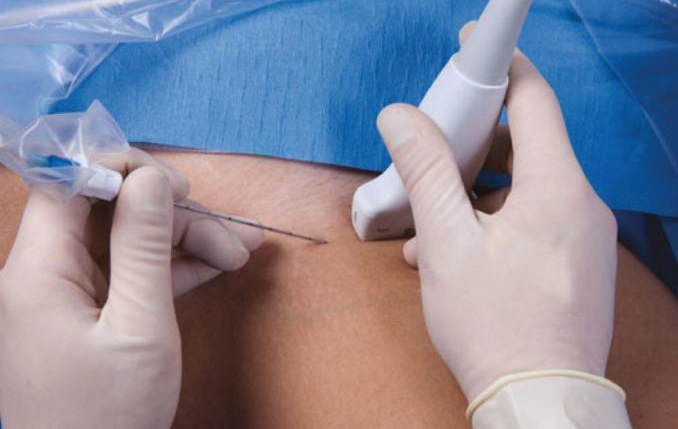
\includegraphics[width=0.5\textwidth]{IMG/RAUS.png}
%     \caption{ Anestesia regional guiada por \acl{US}.}
%   \label{fig:raus}
% \end{figure}
\begin{figure}[h]
   \begin{subfigure}[b]{0.45\linewidth}
        \centering
        {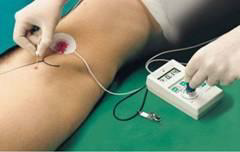
\includegraphics[width=\linewidth]{IMG/electrical.png}}
        \caption{\label{fig:electrical}Anestesia regional guiada por estimulación eléctrica.}
    \end{subfigure}
    \null\hfill
     \begin{subfigure}[b]{0.45\linewidth}
        \centering
        {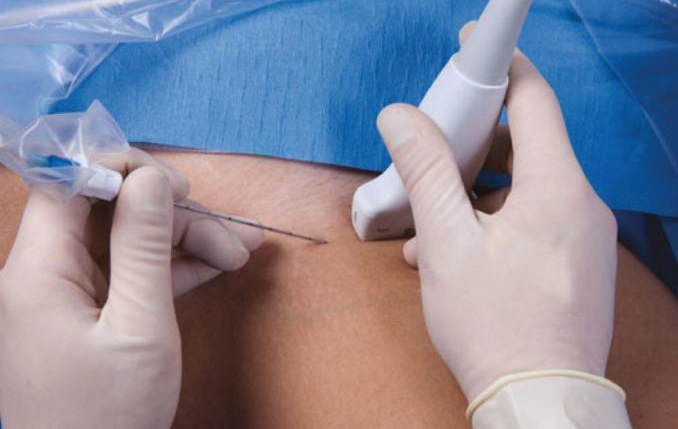
\includegraphics[width=\linewidth]{IMG/RAUS.png}}
        \caption{\label{fig:raus}Anestesia regional guiada por \acl{US}.}
    \end{subfigure}
     
    \caption{Técnicas de \acl{RA}.}
   \end{figure}
   
   
Según la zona anatómica donde se realice, la posición del paciente varía y, por tanto, es importante que el médico deba conocer la disposición del nervio a bloquear. Por ejemplo, el bloqueo femoral es probablemente el bloqueo de extremidad inferior que se realiza con más frecuencia por su facilidad y su alta tasa éxito. En este procedimiento, el paciente se coloca decúbito supino. Sin embargo, en el bloqueo axilar, es necesario que el paciente esté en posición de flexión del brazo por contracción del bíceps.

%\todo{Da más datos bloque del nervio femoral ... }

La ejecución de este procedimiento no es sencilla para aquellos profesionales de anestesiología que no están familiarizados con las técnicas de \ac{US}. Además de los conocimientos teóricos, los profesionales deben entrenar sus habilidades no cognitivas. Estos entrenamientos habitualmente se llevan a cabo con pacientes reales, con la utilización de cadáveres \cite{Tsui2007} o mediante el uso de \emph{fantomas} \cite{phantomra}. La incorporación de un simulador en el entrenamiento del procedimiento ayudará a solventar las limitaciones de los entrenamientos clásicos al ser repetible y seguro.


Según el Entregable 2.1 de \ac{RASimAs} titulado \emph{User Specifications} \cite{ded2.1}, el procedimiento de \ac{RA} guiado por \ac{US} se puede separar en los siguientes bloques:
\begin{enumerate}
    \item Exploración (\emph{Scout Scan}): el profesional configura y explora con la sonda de \ac{US} la zona del paciente con el objetivo de identificar el nervio, vasos sanguíneos cercanos y las demás estructuras anatómicas importantes (figura \ref{fig:scoutscan}). 

%\todo{ Las imágenes se ven fatal, las paso a word, word a pdf y las pongo en el anexo? puedo citarlas también en los resultados}
    \item Guiado de la aguja (\emph{Needle Guidance}): cuando el profesional está seguro de haber interpretado la imagen de \ac{US}, guía la aguja a través de la anatomía hasta aproximarse al nervio (figura \ref{fig:needleguidance}).  
   
    \item Inyección (\emph{Injection}): el médico libera el bolo y confirma que se ha realizado correctamente el bloqueo del nervio (figura \ref{fig:injection}). 
   
\end{enumerate}
\begin{figure}[thbp]
  \centering
    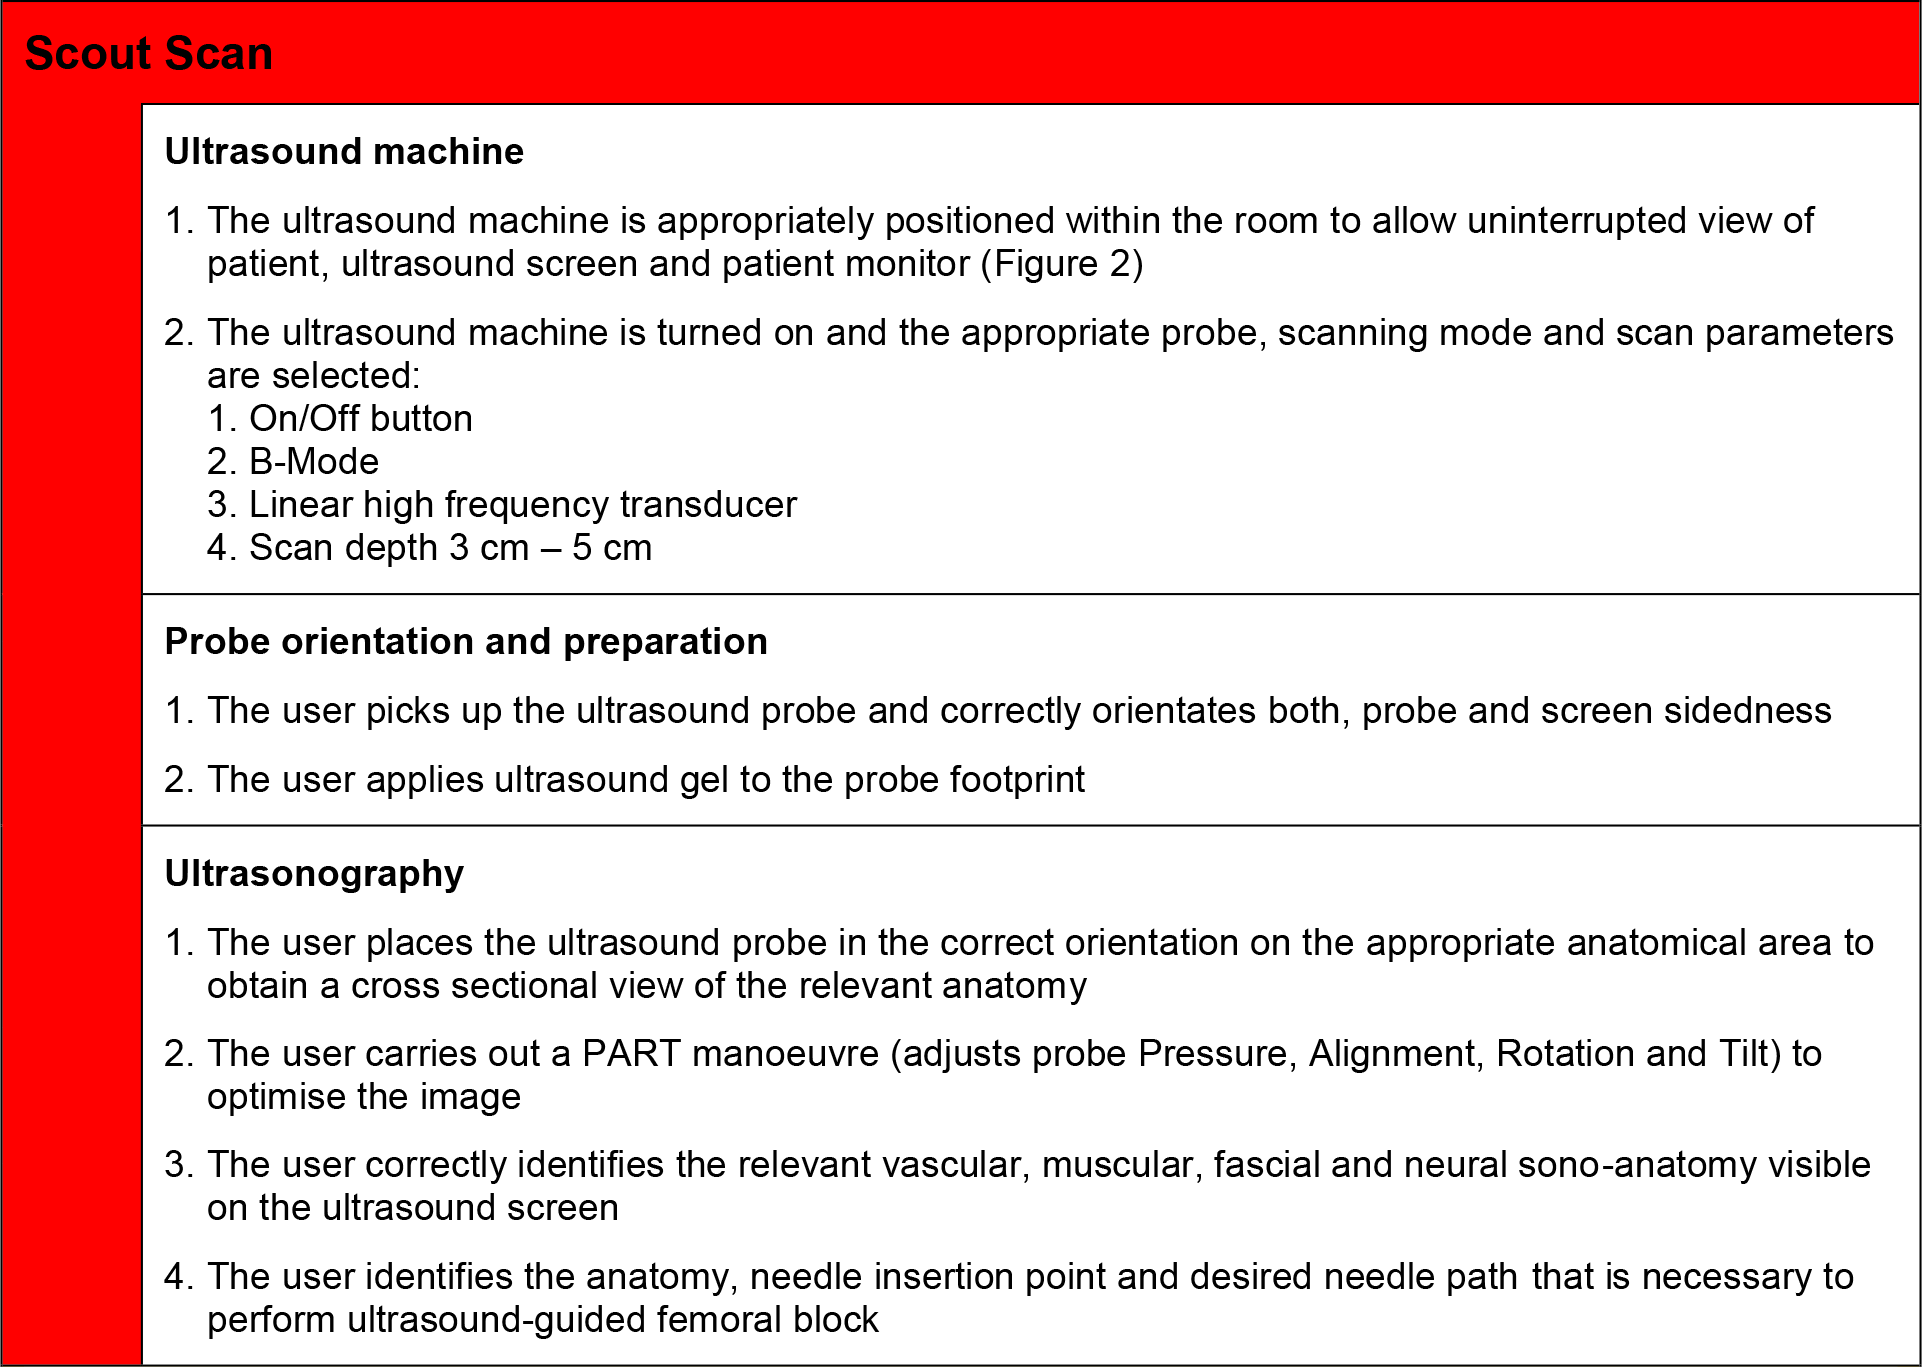
\includegraphics[width=0.8\textwidth]{IMG/scoutscan.png}
    \caption{Tareas del bloque de exploración. }
  \label{fig:scoutscan}
   
\end{figure}
 \begin{figure}[tbhp]
  \centering
    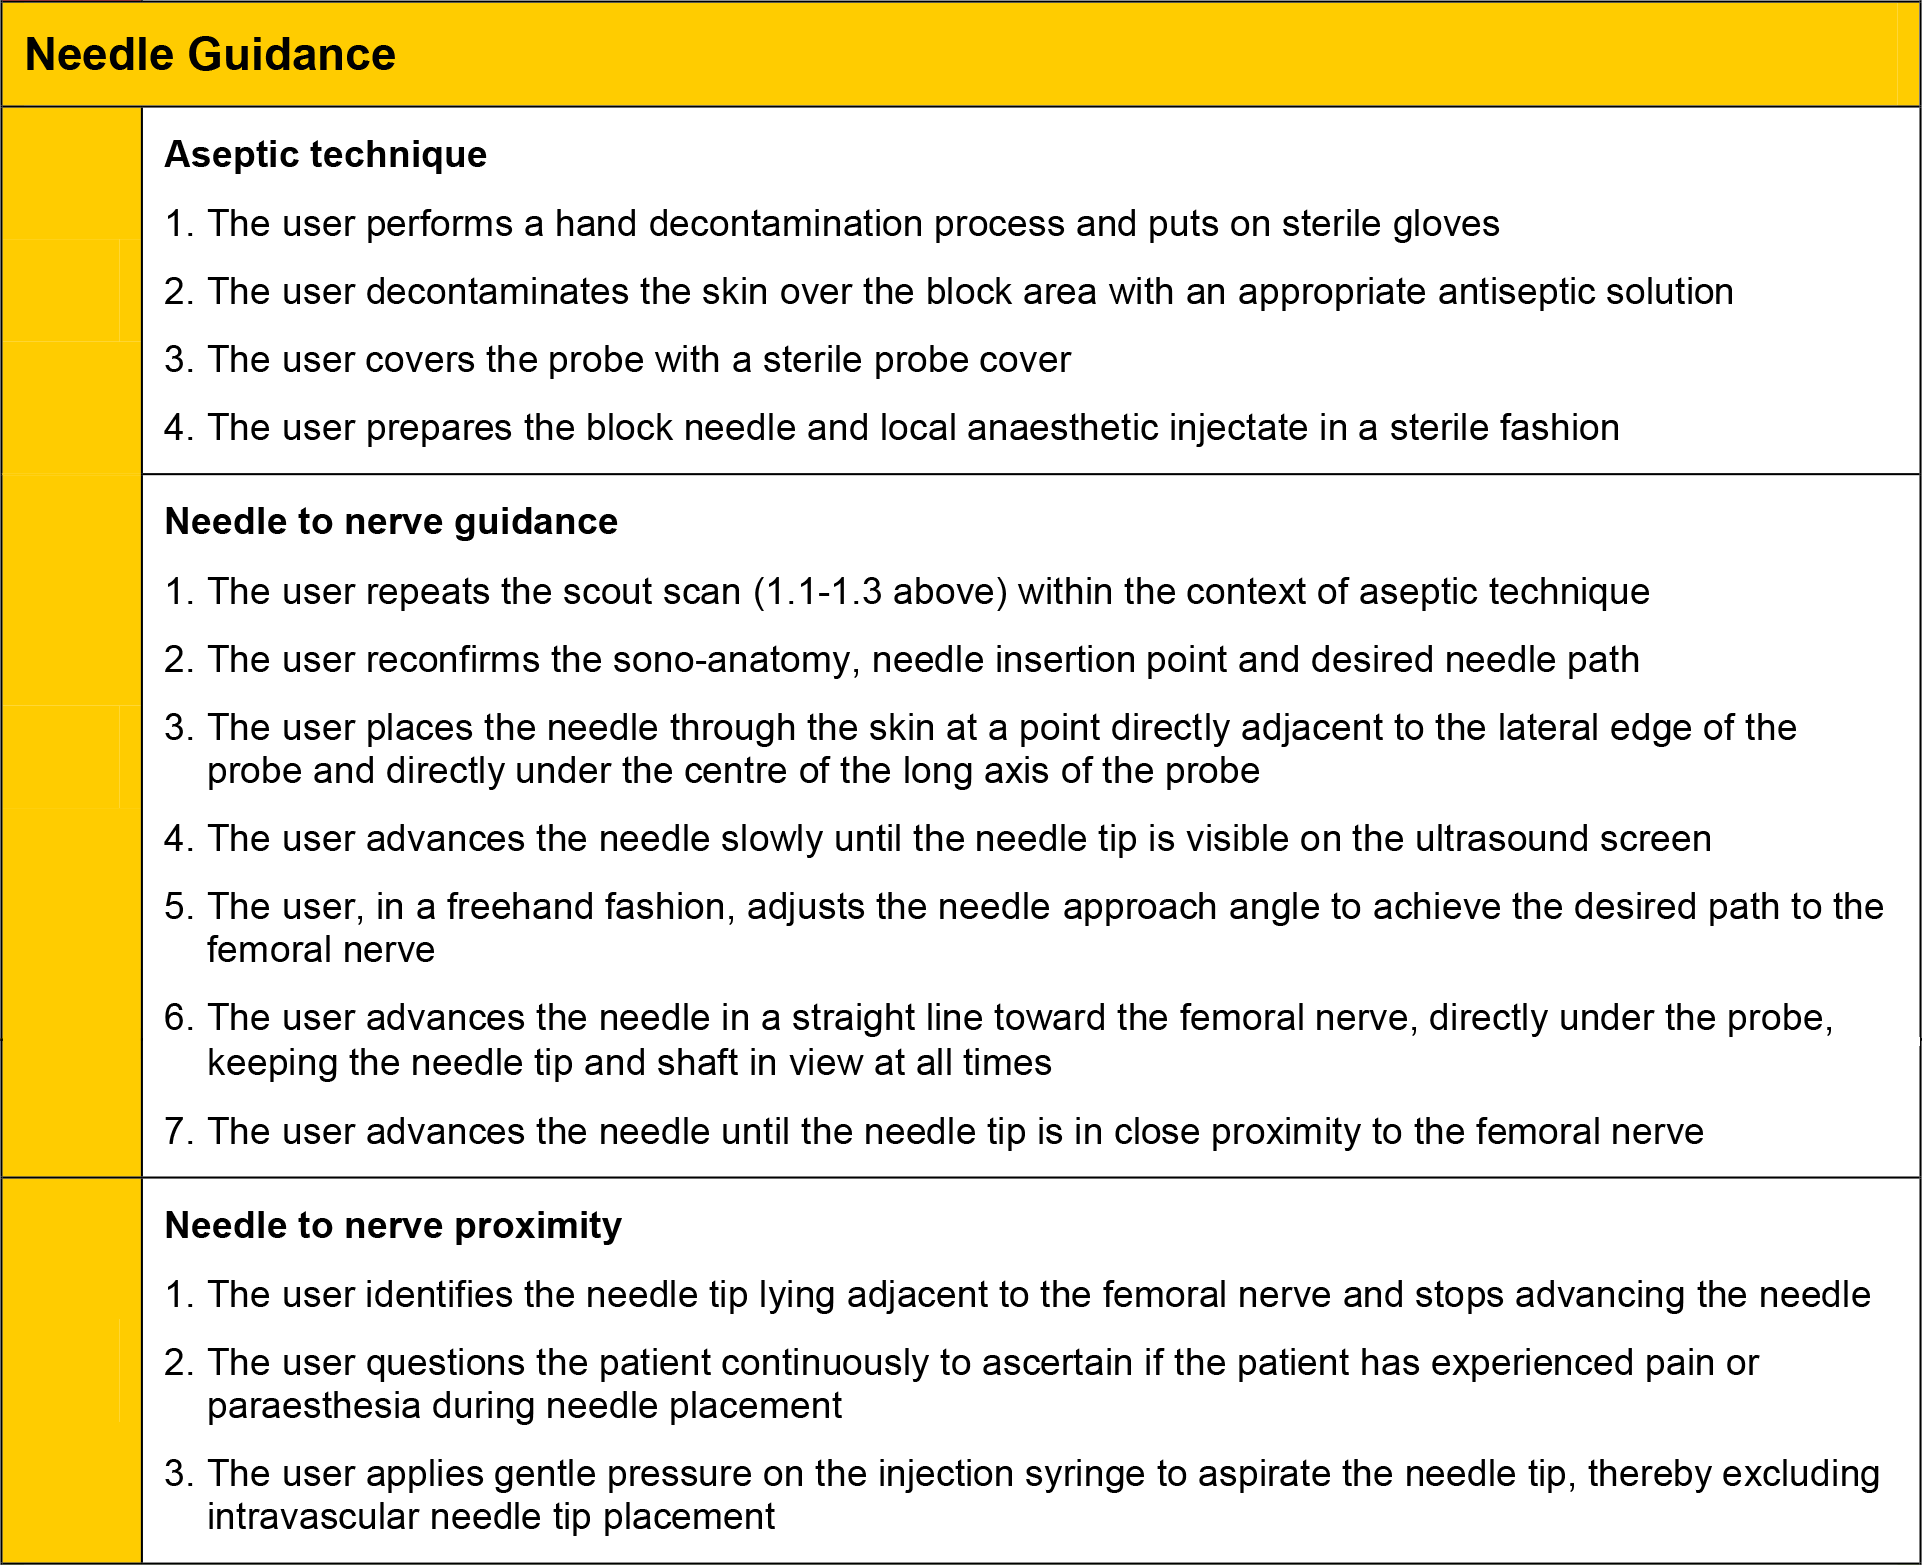
\includegraphics[width=0.8\textwidth]{IMG/needleguidance.png}
    \caption{Tareas del bloque de guiado de la aguja. }
  \label{fig:needleguidance}
\end{figure}

 \begin{figure}[th]
  \centering
    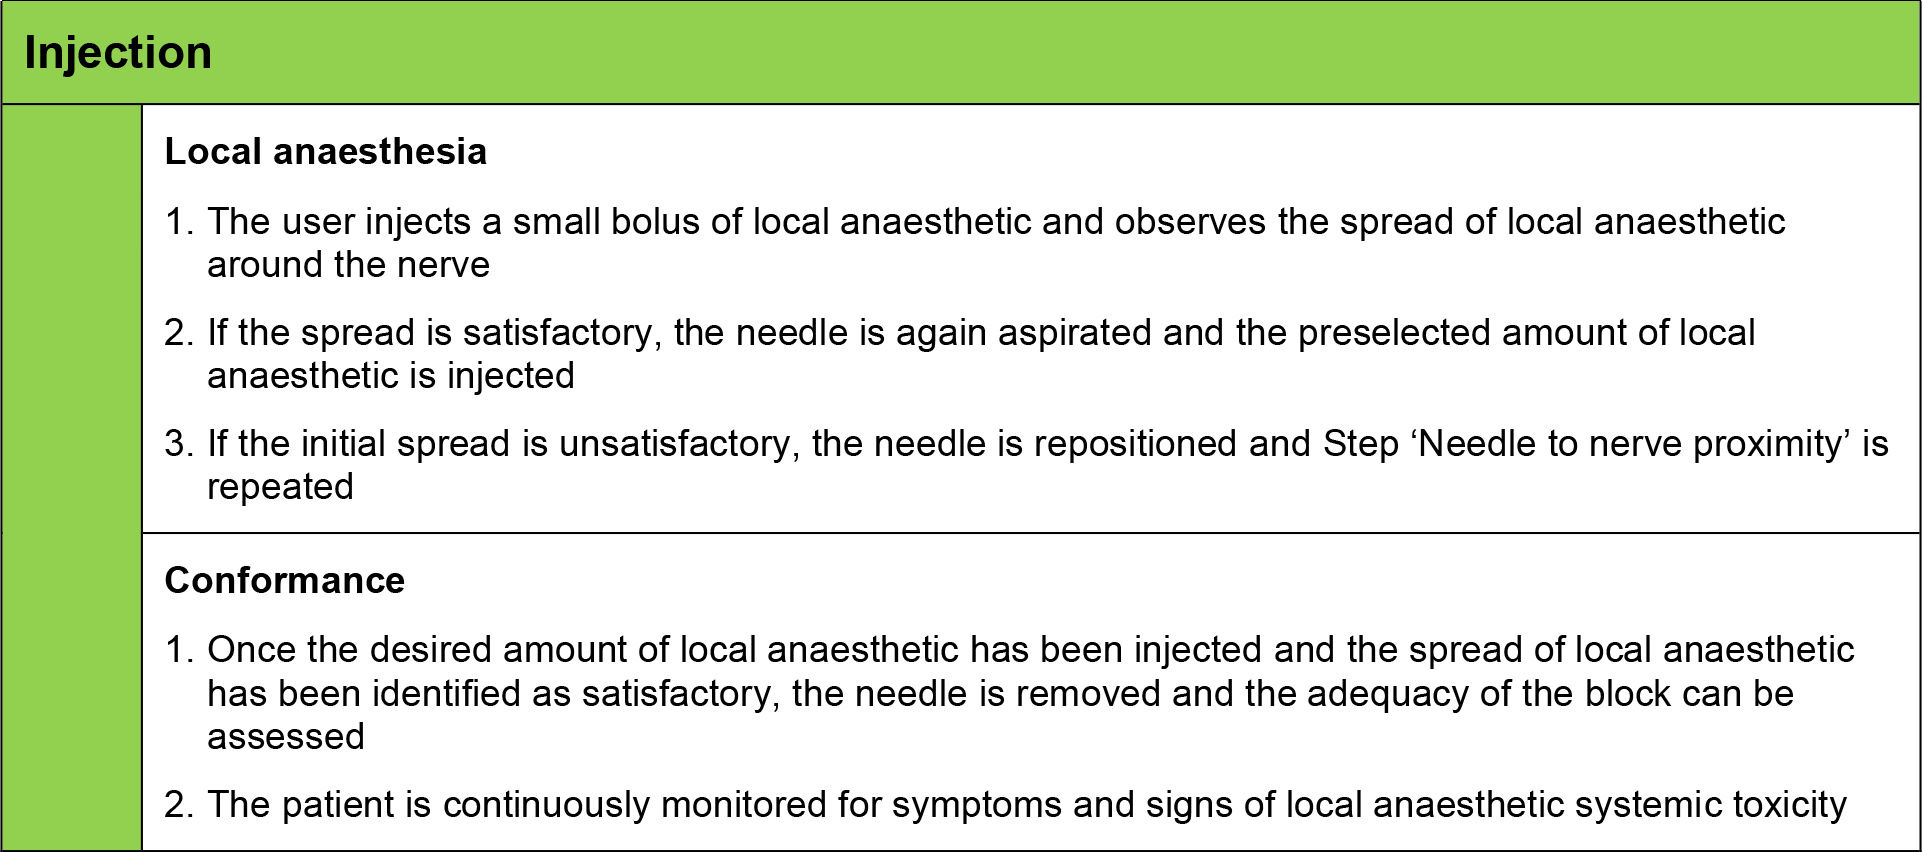
\includegraphics[width=0.8\textwidth]{IMG/injection.png}
    \caption{ Tareas del bloque de inyección.}
  \label{fig:injection}
\end{figure}


% \begin{figure}[h]
%     \begin{subfigure}[b]{0.7\linewidth}
%         \centering
%         {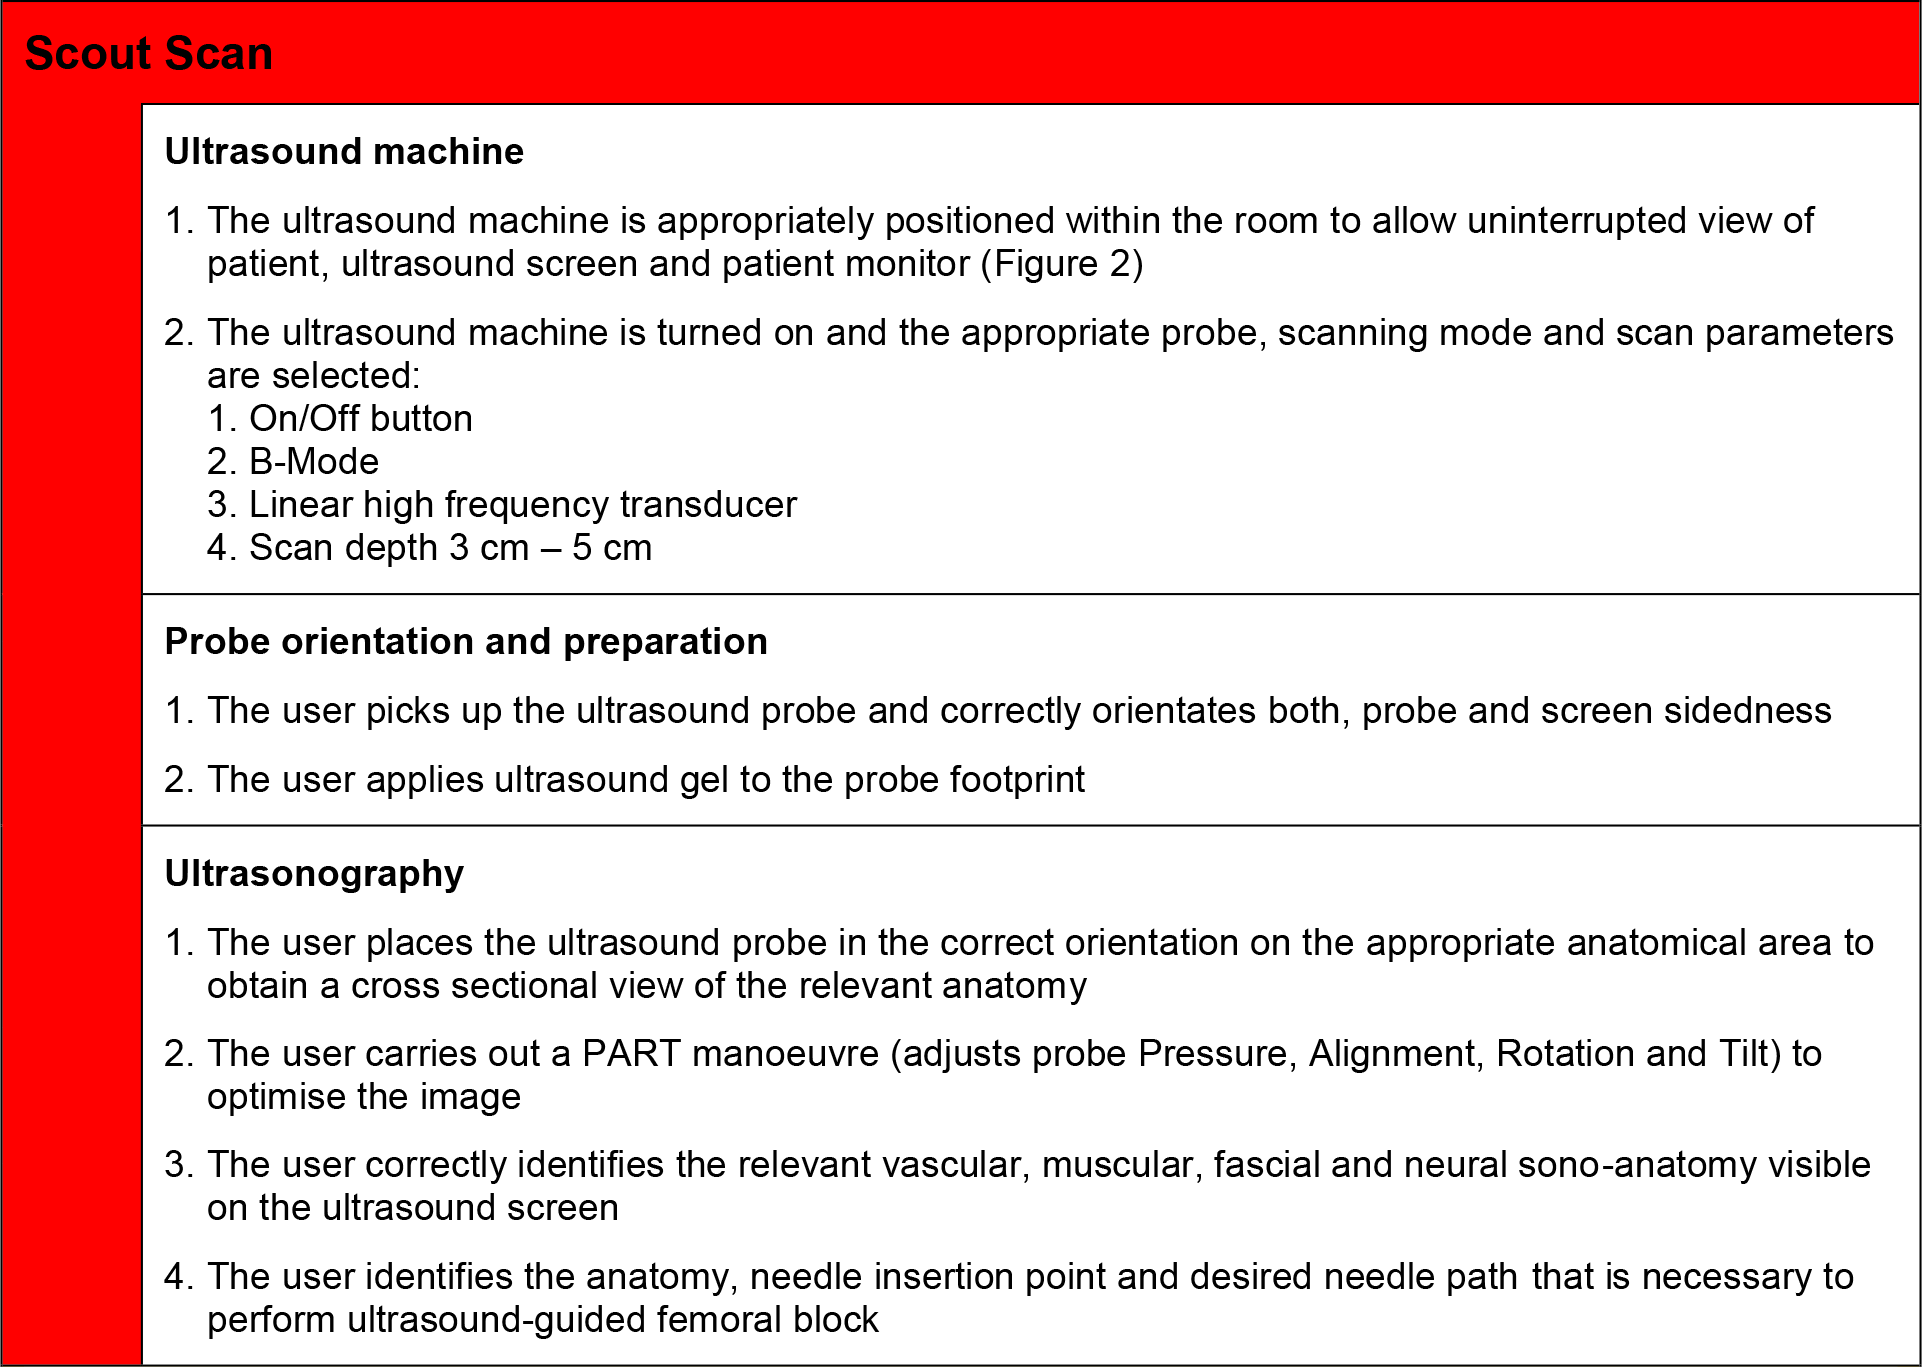
\includegraphics[width=\linewidth]{IMG/scoutscan.png}}
%         \caption{Tareas del bloque de exploración 
%   \label{fig:scoutscan}}
%     \end{subfigure}
%      \begin{subfigure}[b]{0.7\linewidth}
%         \centering
%         {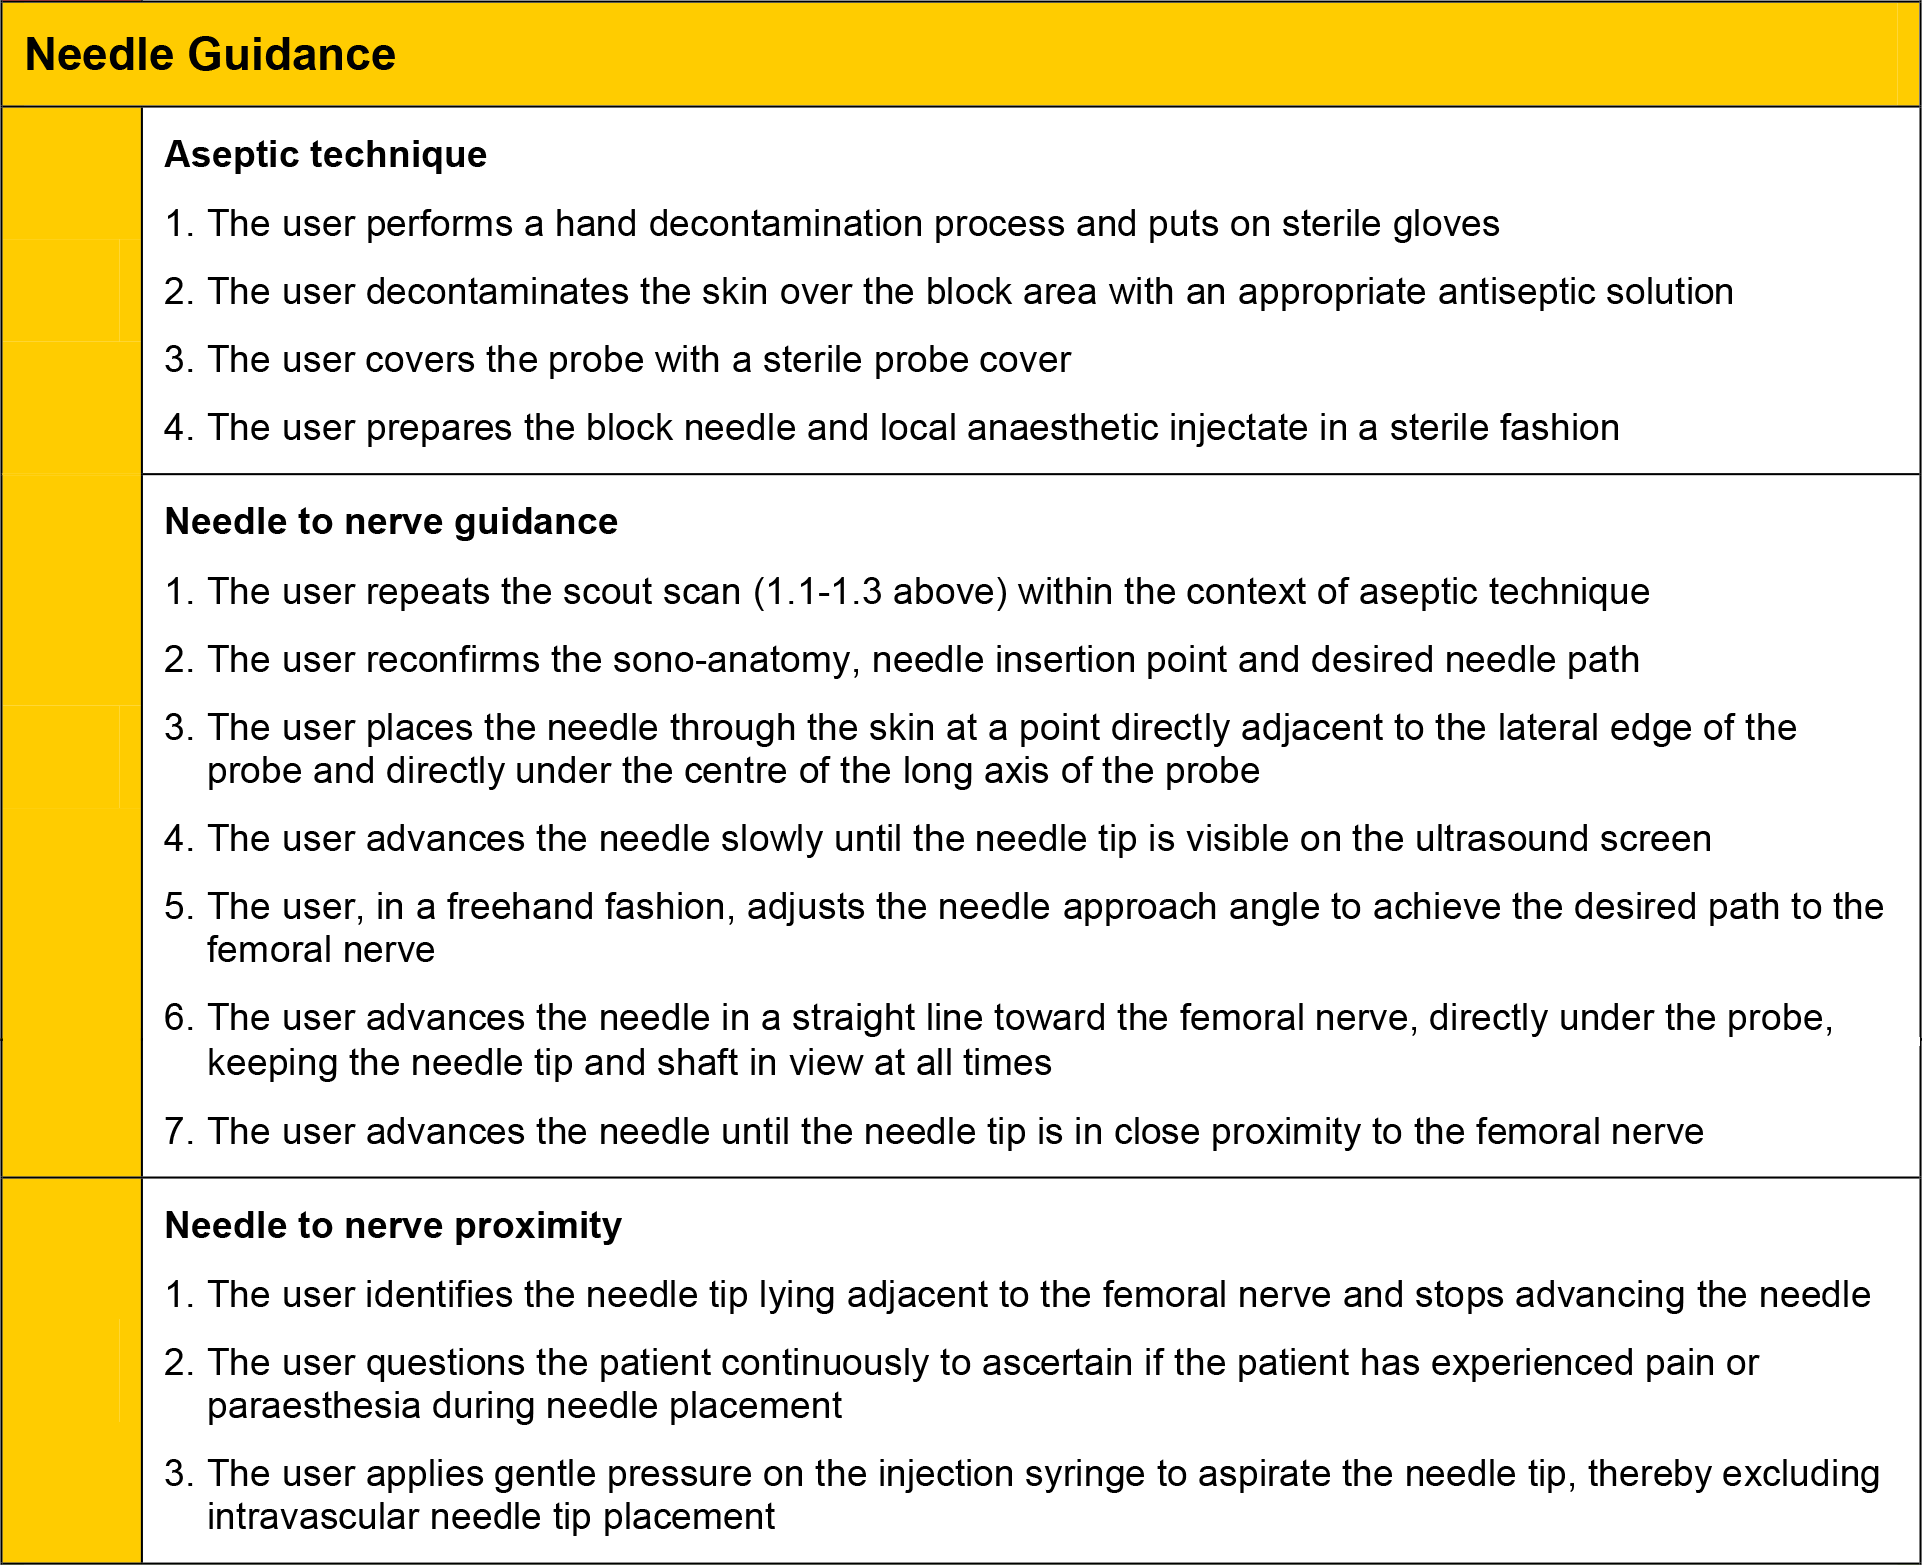
\includegraphics[width=\linewidth]{IMG/needleguidance.png}}
%         \caption{Tareas del bloque de guiado de la aguja. \label{fig:needleguidance}}
%     \end{subfigure}
%      \begin{subfigure}[b]{0.7\linewidth}
%         \centering
%         {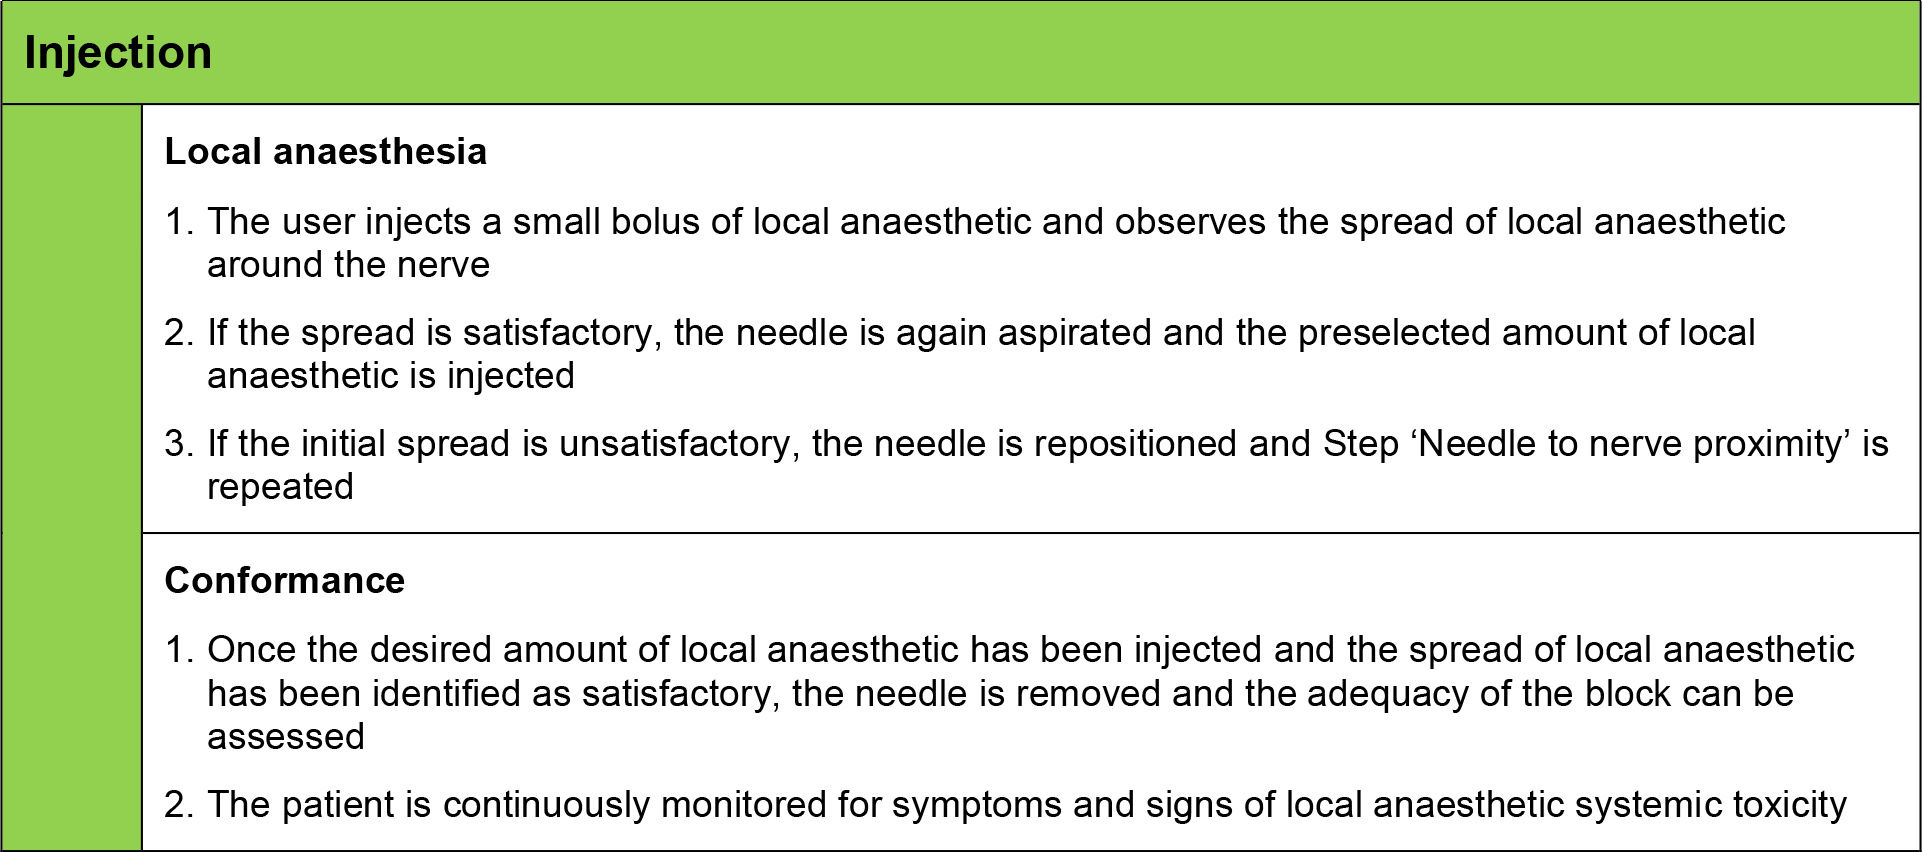
\includegraphics[width=\linewidth]{IMG/injection.png}}
%         \caption{Tareas del bloque de inyección. \label{fig:injection}
%   }
%     \end{subfigure}
%     \caption{Listado del procedimiento completo}
%   \end{figure}
% \clearpage
Con el objetivo de explicar detalladamente cada bloque, se resumirá a continuación el procedimiento completo para un bloqueo femoral:
%
el anestesista deberá posicionarse en la sala de tal forma que su ángulo de visión permita observar al paciente y al monitor de \ac{US} %y al monitor de las constantes vitales
sin mover la cabeza (figura \ref{fig:roomplace}). El médico configurará el equipo de \ac{US} con los valores apropiados y explorará la zona anatómica con la sonda. Para conseguir una imagen adecuada, se procederá a la maniobra PART (del inglés \emph{Pressure, Alignment, Rotation and Tilt}) que permite colocar correctamente la sonda de \ac{US} para asegurar una buena imagen donde se puedan localizar todas las estructuras anatómicas relevantes. Una vez el nervio esté localizado, el médico introducirá la aguja en plano\footnote{La aguja se introduce en paralelo con la proyección ultrasonográfica para que quede totalmente visible en la imagen.} con la sonda de \ac{US}, permitiendo así su visualización en la imagen y la dirigirá hasta la proximidad del nervio. Es entonces cuando antes de inyectar el bolo, deberá aspirar primero para comprobar que la punta de la aguja no se encuentre dentro de un vaso sanguíneo y pueda causar toxicidad sistémica \footnote{El anestésico se distribuirá por los vasos sanguíneos.}. Una vez comprobado, a continuación, solo se distribuirá una pequeña cantidad para asegurarse de la localización de la aguja y por último se liberará el bolo completamente. El profesional deberá confirmar que el bloqueo ha sido satisfactorio y comprobará cualquier síntoma de malestar en el paciente.


\begin{figure}[thbp]
   \centering
    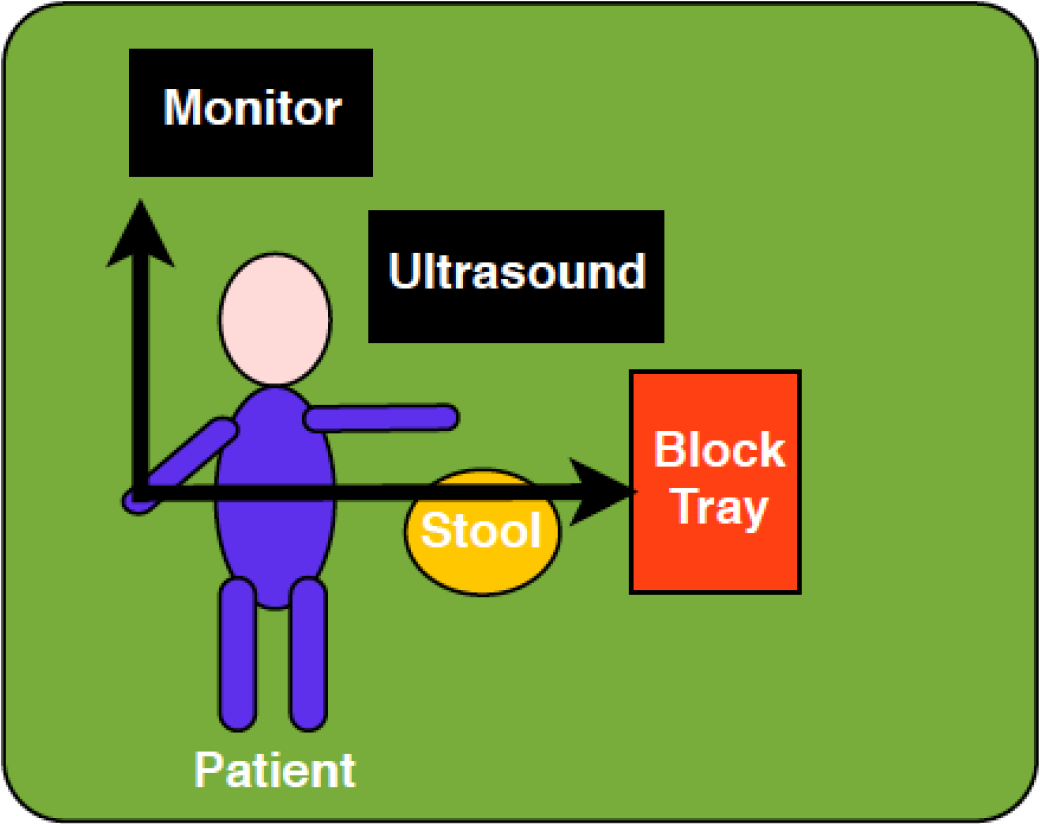
\includegraphics[width=0.5\textwidth]{IMG/roomplacement.png}
    \caption{Diagrama que muestra la disposición del anestesista en la sala de operaciones en un bloqueo femoral. Este se sienta adyacente al paciente, mirando hacia los monitores y con la bandeja de los instrumentos a su derecha.}
   \label{fig:roomplace}
\end{figure}





%https://www.gtsimulators.com/Full-Body-X-Ray-Phantom-with-Real-Human-Skeleton-p/ez7200.htm




% El proyecto \ac{RASimAs} tiene como objetivo  facilitar el entrenamiento y la práctica de la \ac{RA} con la ayuda de un simulador (\ac{RASim}).
% Para que sea utilizado en el mayor número de sitios posibles (hospitales, universidades y colegios profesionales) se debe proporcionar una herramienta de entrenamiento que sea barata, fácil de usar, robusta y que necesite poco mantenimiento.
% Estas herramientas están dirigidas para diferentes perfiles de usuarios.  Tanto estudiantes como profesionales que están empezando a realizar el procedimiento, el simulador les proporcionará un método de entrenamiento con el que mejorar sus habilidades cognitivas y propioceptivas. A su vez, este proyecto también está orientado para profesionales anestesistas que han estado alejados de la práctica del procedimiento y quieran retomar la actividad.
% Los objetivos principales del simulador \ac{RASim} son los siguientes:
% \begin{enumerate}
%     \item El estudiante puede adquirir y desarrollar las habilidades cognitivas y no cognitivas que le permitan ejecutar un bloque de nervio guiado por \ac{US} empezando por el bloqueo del nervio femoral y siguiendo con las siguientes localizaciones.
%     \item Permitir a un anestesista retomar y practicar las habilidades necesarias para realizar el procedimiento de forma segura y satisfactoria.
%     \item Recuperar y medir métricas de rendimiento al realizar el procedimiento en el simulador. 
%     \item Permitir a un supervisor revisar las métricas registradas por los usuarios del simulador a través del tiempo
% \end{enumerate}







%\subsubsection{Objetivos del simulador}


% 6.1.3 Principles of use
% 1. RASim must be contextually relevant and function within the existing or evolving regional
% anaesthesia curriculum
% 2. RASim training must be based upon appropriately detailed characterised procedures
% 3. RASim training must allow the development of relevant procedural skills and associated
% clinical decision making
% 4. RASim training must never allow the development of procedural skill relevant only within
% the simulation environmentRASim training should allow performance related feedback, repeated practice and
% performance tracking and progression over time each based on precisely defined metrics
% 6. RASim based training programmes must have a defined beginning and end (entry and
% exit) constituting proficiency based progression for defined applications e.g. independent
%practice , supervised practice


\subsection{Diagnóstico por imagen médica}
\label{art:xraysim}

Dentro de la medicina, hay multitud de técnicas y procesos que generan imágenes médicas (\ac{US}, \ac{TC}, \ac{IRM}, etc.)  utilizadas para el diagnóstico de enfermedades, afecciones o dolencias. %Existen multitud de técnicas anteriormente mencionadas 
Su utilización depende de la tecnología en las que están basadas, ya que capturan diferentes tejidos o imágenes.
%Esto caracteriza su utilización dependiendo de que tejidos o que imágenes se capturan del cuerpo del paciente. 

El segundo caso de uso que se presenta en esta tesis está orientado al diagnóstico por imagen generada con rayos X. Esta especialidad médica se centra en la generación e interpretación de imágenes que se consiguen al exponer la anatomía objetivo a una radiación electromagnética que será recogida por un detector. Años atrás, se proyectaba sobre películas fotográficas especialmente preparadas para la fuente emisora. Sin embargo, actualmente la mayoría de las imágenes son almacenadas digitalmente gracias a un detector que permiten guardarlas directamente en un computador.

Se denominan proyecciones radiológicas al procedimiento de situar tanto al paciente como el equipo de radiología para conseguir una imagen de una parte concreta de la anatomía del paciente. Esta técnica define una proyección por cada parte del cuerpo a diagnosticar, requiere por cada procedimiento una postura del paciente y una configuración del equipo de radiografía concreta.

Según el libro \cite{manualpractico}, el procedimiento habitual que se debe seguir se resume en los siguientes pasos:
\begin{enumerate}
    \item Elección de \emph{Bucky}: elemento para reducir la radiación no perpendicular al detector. Este filtro suele utilizarse siempre, excepto en condiciones de emergencia o limitaciones físicas.
    \item Tamaño del chasis y orientación: colocar el detector de la manera que permita cubrir la anatomía a estudiar.
    \item Posición del paciente: teniendo en cuenta las limitaciones del paciente, se le debe posicionar de pie, sentado o decúbito.
    \item Posición de la región anatómica: 
    se colocará al paciente de tal forma que la región objeto de estudio se sitúe correctamente centrado en el chasis.
    \item Distancia-foco película: se sitúa el emisor de rayos X a la distancia adecuada para la proyección.
    \item Angulación: existen algunas proyecciones donde el chasis se inclina para evitar superposición de estructuras.
    \item Centraje: se centra la proyección de los rayos X en el centro de la región anatómica a estudiar, para lo que es fundamental el conocimiento de la anatomía.
    \item Colimación: se reduce la apertura de la radiación para reducir la exposición del paciente.
    \item Técnica aproximada: se configurará la potencia del equipo de radiología con el objetivo de reducir los niveles de exposición a lo mínimo posible, manteniendo la calidad diagnóstica (principio ALARA del inglés \emph{As Low As Reasonably Achievable} \cite{manualpractico}). 
    \item Indicaciones al paciente: se trata de las órdenes que se le dan al paciente en el momento de tomar la imagen.
\end{enumerate}

Al igual que se indica en \cite{manualpractico}, esta metodología, y en concreto los valores de potencia de los emisores de radiación, no es estándar y es susceptible de variaciones dependiendo generalmente del centro de trabajo, profesionales, escuelas, rendimiento y antigüedad de los equipos, etcétera. 



%https://www.bluephantom.com/product/Sciatic-Nerve-Regional-Anesthesia-Ultrasound-Training-Model.aspx?cid=428
\section{Contexto en RASimAs}
\label{art:rasimas}

% El \ac{WP} 3 del proyecto \ac{RASimAs} tiene como objetivo crear \nuevo{un} modelo virtual con anatomía especifica de pacientes. Con el objetivo de conseguir el máximo realismo posible, se propone como objetivo crear modelos virtual que pueda usarse en el simulador que contenga anatomía real de pacientes. Para ello se propone crear la herramienta \ac{TPTVPH}.
% Este juego de herramientas está diseñado para permitir crear un \ac{VPH} y que pueda ser posicionado y movido durante su uso en el simulador.

% Para lo cual, debido a su complejidad el \ac{WP} se divide en varias tareas.
% \begin{itemize}
%     \item Tarea 3.1 Adquisición de datos:
%         A partir de imágenes de \ac{IRM}, \ac{TC}, etc... se conseguirá un modelo virtual que servirá como entrada para las tareas siguientes.
%     \item Tarea 3.2 Modelado anatómico:
%         Finalización de los modelos superficiales de los tejidos que se han recuperado de la tarea anterior.
%     \item Tarea 3.3 Modelado mecánico:
%         El objetivo es conseguir o modelar el comportamiento mecánico de los tejidos como los músculos 
%     \item Tarea 3.4 Modelado fisiológico:
%         Esta tarea está focalizada en crear el comportamiento de los nervios y el consecuente movimiento de los músculos. 
%     \item Tarea 3.5 Integración:
%         Con el resultado de todas las tareas anteriores, es posible automatizar y crear una herramienta para que partiendo de las imágenes iniciales pueda crearse un paciente virtual.
%     \item Tarea 3.6 Posicionamiento de pacientes:
%         Por último, es necesario modificar la posición del paciente a la posición requerida por \ac{RA}. 
% \end{itemize}

% \begin{figure}[h]
%   \centering
%     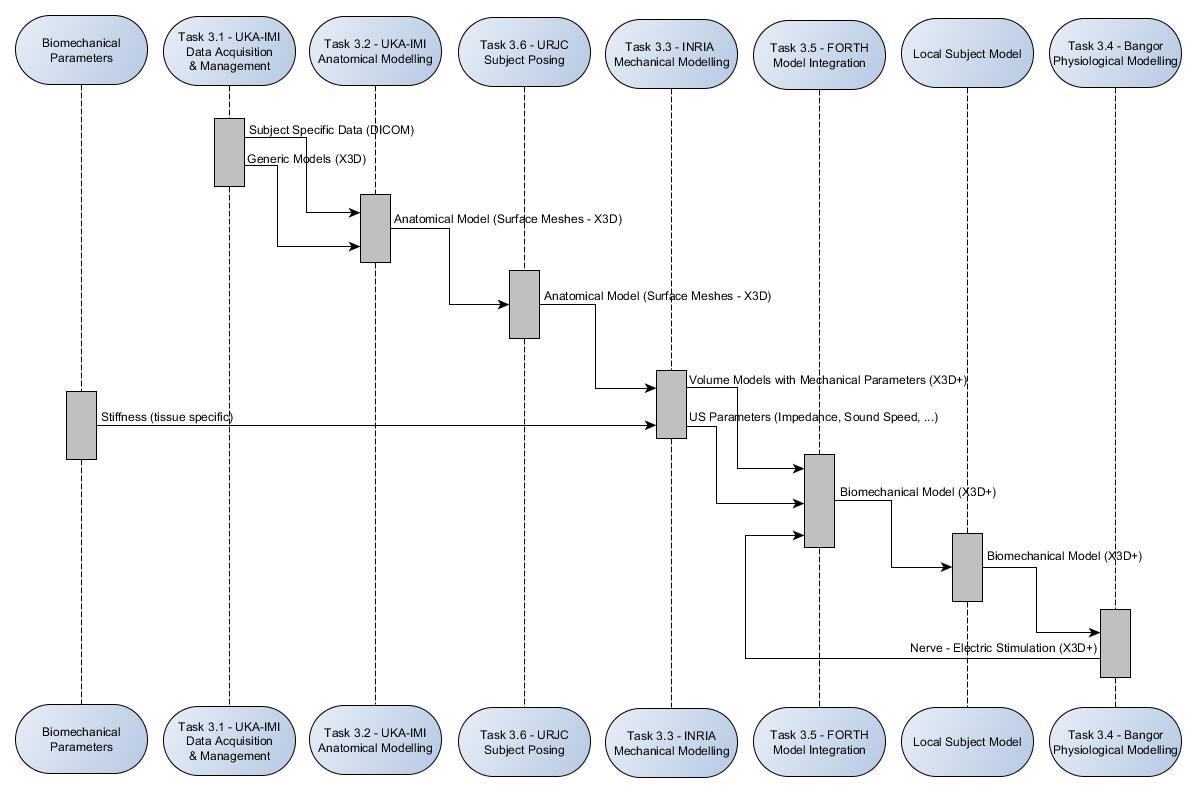
\includegraphics[width=0.5\textwidth]{IMG/RASimAs_D3.png}
%     \caption{ }
%   \label{fig:WP3}
% \end{figure}


% Por tanto, la tarea 3.6 necesita crear un método que sea capaz de modificar la posición de un paciente virtual a su posición final, de manera que pueda usar todos o varios resultados intermedios de las tareas anteriores a esta. Como parte de ese trabajo, esta tesis presenta una solución que se centra en resolver de manera innovadora los problemas encontrados.

% \todo{meter wp 5?}


%\todo{ En ese capitulo lo primero que tienes que contar es que este simulador da la opción de probar el posing. Permitiendo comprobar si los resultados son suficientemente buenos para ser usados para entrenamiento. Indicar que de cara a construir un simulador completo el proyecto se estructuro en paquetes de trabajos. Pon una sección donde expliques los paquetes de trabajo donde se desarrollaron los módulos relevantes del simulador y cual fue tu contribución a cada uno. En el resto del capitulo detalla esta contribución.}

El proyecto \ac{RASimAs} tiene como objetivo  facilitar el entrenamiento y la práctica de la \ac{RA} con la ayuda del simulador \ac{RASim} y el asistente \ac{RAAs}. El trabajo realizado en esta tesis ha estado centrado en el simulador.


Para fomentar su uso en el mayor número de sitios posibles (hospitales, universidades y colegios profesionales), se debe proporcionar una herramienta de entrenamiento que sea barata, fácil de usar, robusta y que necesite poco mantenimiento. Además, el simulador debe estar dirigido para diferentes perfiles de usuarios. Tanto a estudiantes como a profesionales que están empezando a realizar el procedimiento, el simulador les proporcionará un método de entrenamiento con el que mejorar sus habilidades cognitivas y propioceptivas. A su vez, este proyecto también está orientado para profesionales anestesistas que han estado alejados de la práctica del procedimiento y quieran retomar la actividad.


Se han definido unos objetivos principales del simulador \ac{RASim}:
\begin{enumerate}
    \item El estudiante puede adquirir y desarrollar las habilidades cognitivas y no cognitivas que le permitan ejecutar un bloque de nervio guiado por \ac{US} empezando por el bloqueo del nervio femoral y siguiendo con las siguientes localizaciones.
    \item Permitir a un anestesista retomar y practicar las habilidades necesarias para realizar el procedimiento de forma segura y satisfactoria.
    \item Recuperar y medir métricas de rendimiento al realizar el procedimiento en el simulador. 
    \item Permitir a un supervisor revisar las métricas registradas por los usuarios del simulador a través del tiempo.
\end{enumerate}



Como se introdujo en la sección \ref{intro:rasimas}, el proyecto \ac{RASimAs} se dividió en \acl{WP} (ver figura \ref{fig:wp_rasimas}) donde los \ac{WP} 3, 4 y 5 se centraban en el desarrollo de los prototipos \ac{RASim} y \ac{RAAs}. 
A continuación, se van a introducir brevemente las tareas de estos \acl{WP} y nombrar aquellos en los que ha contribuido de manera activa la \ac{URJC}, donde se encuadra la mayor parte de la investigación realizada en esta tesis. 

%\todo{vuelvo a poner la imagen?}

\begin{itemize}
%\todo{Frase mal redactada.  No has hablado de la importancia de crear una base de datos de pacientes. Recuerda resaltar que no se buscan pacientes reales sino pacientes promedio con distinta variabilidad.}
    \item 
El \ac{WP} 3 del proyecto \ac{RASimAs} tiene como objetivo crear la \emph{suite} \ac{ITGVPH}. Se integrará un conjunto de aplicaciones que servirán para generar una base de datos de \ac{VPH}, con el objetivo de conseguir un entrenamiento con una gran variabilidad anatómica. Además, se permite que el paciente virtual pueda ser adaptado a la postura que se requiera según el procedimiento que se esté realizando. Este paquete se ha dividido en las siguientes tareas:%Este paquete se divide en seis tareas lideradas por \ac{UKA-IMI}. }
\begin{enumerate}
    \item \textbf{Adquisición de datos:} análisis y recopilación de imágenes médicas que serán utilizadas para la creación de los \ac{VPH}.
    \item \textbf{Modelado anatómico:} se realiza un registro entre las imágenes médicas y modelos anatómicos comerciales con el objetivo de generar nuevos modelos anatómicos.
    Tanto la tarea anterior como esta fueron asignadas a \ac{UKA-IMI}.
    \item \textbf{Modelado mecánico:} se generan los modelos mecánicos que se utilizarán en la simulación física del simulador. Este módulo ha sido asignado al \ac{INRIA}.
    \item \textbf{Modelado fisiológico :} en esta tarea se modelará el comportamiento físico de los tejidos cuando los nervios son electroestimulados.
    Tarea asignada a \ac{Bangor}.
    \item \textbf{Herramienta de posicionamiento de pacientes:} este módulo permite adaptar la postura de los modelos anatómicos con todos sus tejidos asociados a la pose requerida por el simulador. Tarea desarrollada en \ac{URJC}, siendo la principal línea de investigación de la presente tesis. En esta tarea, se ha diseñado la aplicación \ac{TPTVPH} que será integrada dentro de la herramienta \ac{ITGVPH}.
    \item {\textbf{Integración:}
    esta tarea asignada a \ac{FORTH}, es la encargada de hacer la integración de todos los módulos anteriores en una única herramienta, ocultando los detalles técnicos a los futuros usuarios.}
\end{enumerate}
{Además de haber participado en las tareas asignadas a la \ac{URJC}, se ha participado activamente en la tarea 3.6, que se encarga de la comunicación de las tareas anteriores.}

% \begin{figure}[h]
%   \centering
%     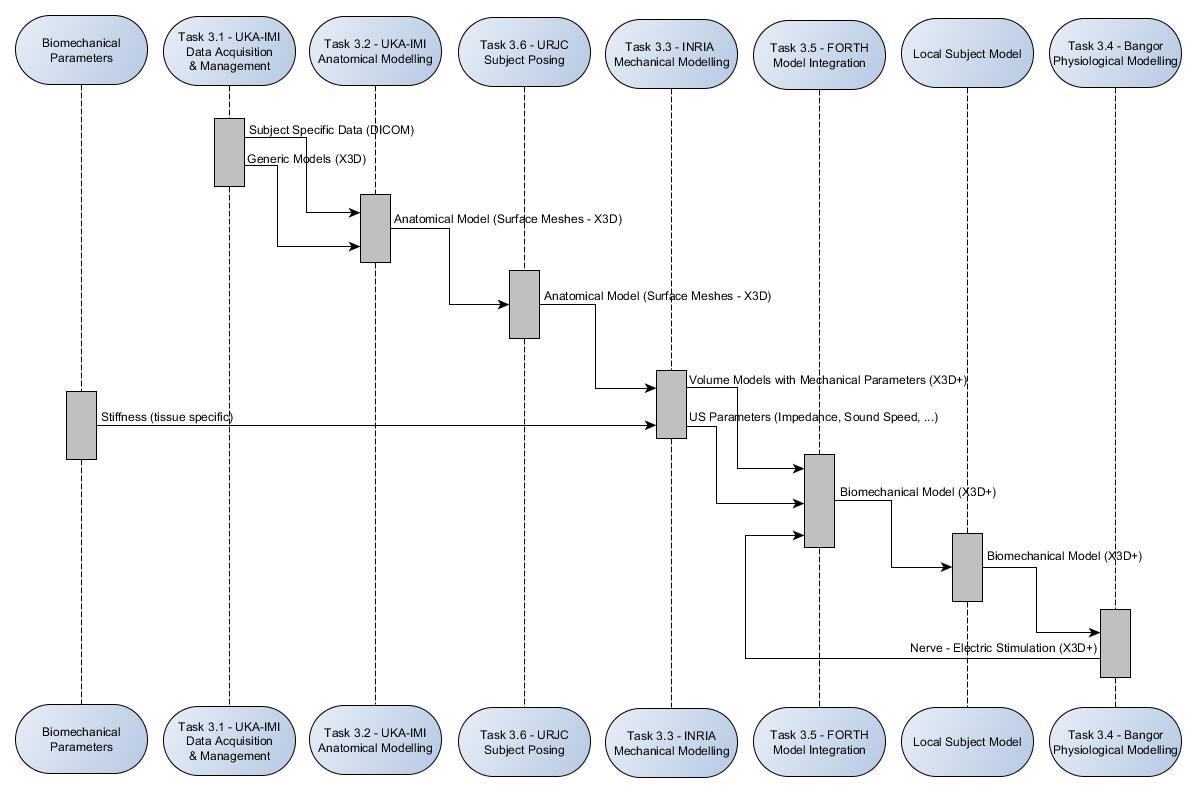
\includegraphics[width=0.9\textwidth]{IMG/RASimAs_D3.png}
%     \caption{ Diagramade secuencia que muestra la organización del \ac{WP} 3 }
%   \label{fig:WP3}
% \end{figure}
%Uno de los módulos clave es un posicionador \todo{no inventes palabras } de pacientes que sea capaz de deformar\todo{adaptar} modelos anatómicos que contengan todo tipo de tejidos \del{externos o internos} para adecuarlos a la posición requerida por el simulador.\todo{indicar cual es la pose de partida. No has dicho en ningún momento que se usan imagenes medicas en poses determinadas. No hables de pacientes reales, habla de imagenes medicas de pacientes reales}
 %\todo{indica el numero de la tarea y di que la lideró la URJC}
\item
El \ac{WP} 4 define las tareas para el desarrollo de los componentes que formarán parte de los prototipos de \ac{RASimAs}. Por una parte, los componentes pertenecientes a \ac{RASim} se definen en las tareas de la 1 a la 4. Por otra parte, los componentes del asistente \ac{RAAs} se definen en las tareas 5 y 6. Estas tareas son las siguientes:

\begin{enumerate}
    \item \textbf{Retroalimentación háptica:}
    desarrollo del algoritmo que permite devolver una respuesta háptica al dispositivo que simula la aguja. Esta tarea fue asignada a \ac{INRIA}.
    \item \textbf{Simulación física:}
    este módulo desarrollado por \ac{INRIA} simula las deformaciones en los tejidos producidas por los instrumentos quirúrgicos.
    \item \textbf{Simulación de \ac{US}:}
    la \ac{RWTH} fue la encargada de desarrollar el módulo que simula la generación de la imagen de \ac{US}.
    \item \textbf{Plataforma de entrenamiento:}
    esta aplicación se comunica con todos los módulos anteriores con el objetivo de proporcionar una aplicación de entrenamiento y autoevaluación. Esta tarea fue asignada a la \ac{URJC} y es una de las contribuciones de esta tesis.
    \item \textbf{Modelado en tiempo real:} esta tarea, perteneciente a \ac{RAAs}, se basa en reconstruir un modelo virtual a partir de las imágenes de \ac{US}. El asistente \ac{RAAs} mostrará estos modelos como ayuda adicional en el procedimiento.
    \item \textbf{Guiado en el procedimiento:}
    el asistente proporcionará ayuda al anestesista durante la intervención, ya que el sistema muestra información sobre la imagen de \ac{US}.
    Tanto la tarea anterior como esta fueron asignadas a \ac{SINTEF}.
\end{enumerate}

Debido a la importancia del \ac{Courseware}, el autor de esta tesis ha participado en las tareas 1, 2, y 3. Este módulo se comunica y gestiona con todos los módulos del simulador.%La importancia de la plataforma de entrenamiento ha dado lugar a participar en las tareas 1, 2 y 3 debido a que el \ac{Courseware} se comunica y gestiona todos los módulos de \ac{RASim}.

%\todo{Indica las tareas y en cuales has estado involucrado. Indicar cuales se han liderado.}

\item
El \ac{WP} 5 se centra en la integración y desarrollo de los prototipos del simulador \ac{RASim} y el asistente \ac{RAAs}. %En el \ac{WP} 6 El objetivo es crear los prototipos con intención de comprobar su validez en evaluaciones clínicas (\ac{WP} 6) con vistas a su posterior comercialización.
\begin{itemize}
    \item {\textbf{Tareas 1 y 2: } integración y construcción del prototipo \ac{RASim} a cargo de \ac{SG}. 
    }
     \item {\textbf{Tareas 3 y 4: } integración y construcción del prototipo del asistente \ac{RAAs} a cargo de \ac{SINTEF}.
    }
\end{itemize}

{Al igual que el \ac{WP} anterior, la importancia del \ac{Courseware} en el prototipo \ac{RASim} hace que se haya trabajado conjuntamente con \ac{SG} para el desarrollo e integración de todos los módulos del simulador. También se contribuyó al proponer una solución con \acs{tracker}s magnéticos ante los problemas encontrados con los dispositivos hápticos.}



\end{itemize}

\section{Animación de la anatomía humana} 
\label{art:anatomy}


%\subsection{Introducción}

Una de las necesidades básicas que debe cubrir un simulador es poder mostrar información anatómica de pacientes virtuales con la que trabajará el usuario. En  \cite{preim2018survey} se explica la necesidad de que los estudiantes tengan un conocimiento profundo de la anatomía humana, estructuras, su posición relativa, variabilidad, etcétera. Es fundamental que un médico cuente con esos conocimientos previamente a la realización del entrenamiento médico.

Existen dos formas comúnmente utilizadas para representar modelos tridimensionales por computador. Tradicionalmente, se utiliza una malla compuesta por facetas poligonales 2D (triángulos o rectángulos) que representa solo la superficie o contorno del modelo sin tener en cuenta ninguna información interna. Estas representaciones se llaman comúnmente \acp{B-rep}. En el momento de \emph{renderizar} se proyecta la geometría y se calcula su iluminación sin interaccionar con el interior del modelo.
% Lo más habitual es utilizar una malla poligonal que define la superficie o contorno del modelo que se representa. Estas mallas están normalmente compuesta por triángulos o rectángulos (quads), comúnmente llamadas \ac{B-rep}. Estas mallas son utilizadas para representar solo la superficie del modelo sin tener en cuenta ninguna información interna.  % \del{Esta malla generalmente está compuesta de polígonos llamados facetas o caras que son la unidad básica de un modelo tridimensional. Las caras más comunes son: triángulos, siendo este el polígono más simple; o rectángulos, que normalmente se descomponen en dos triángulos. El triángulo es la figura más utilizada debido a su menor complejidad matemática en los diferentes cálculos relacionados con la informática gráfica (interpolaciones, manejo de vecinos, etc.).}
%A lo largo del tiempo, las tarjetas gráficas se han diseñado con especial énfasis en el tratamiento de triángulos.
%Por otra parte, existe otro tipo de representación, llamada volumétrica, que permite una representación visual completa de un objeto tanto del exterior como del interior, que la representación poligonal no era capaz. Sin embargo, esto produce una gran complejidad al intentarlas \emph{renderizar} mediante técnicas de imagen generada por computador.

Por el contrario, 
existe otro tipo de representaciones  llamadas volumétricas. Los objetos volumétricos pueden ser representados como una pila de imágenes 2D (\emph{stack} de imágenes), mallas de poliedros, o una imagen  tridimensional formada por \emph{vóxeles}\footnote{Unidad cúbica mínima para representaciones volumétricas.}. A la hora de \emph{renderizar} estas representaciones, existen una variedad de técnicas más complejas (p. ej. técnica \emph{ray casting} \cite{isabel}) para \emph{renderizar} modelos volumétricos.


En la figura \ref{fig:HVP} se puede apreciar dos \emph{renderizados} del mismo modelo anatómico.

\begin{figure}[ht]
   \centering
    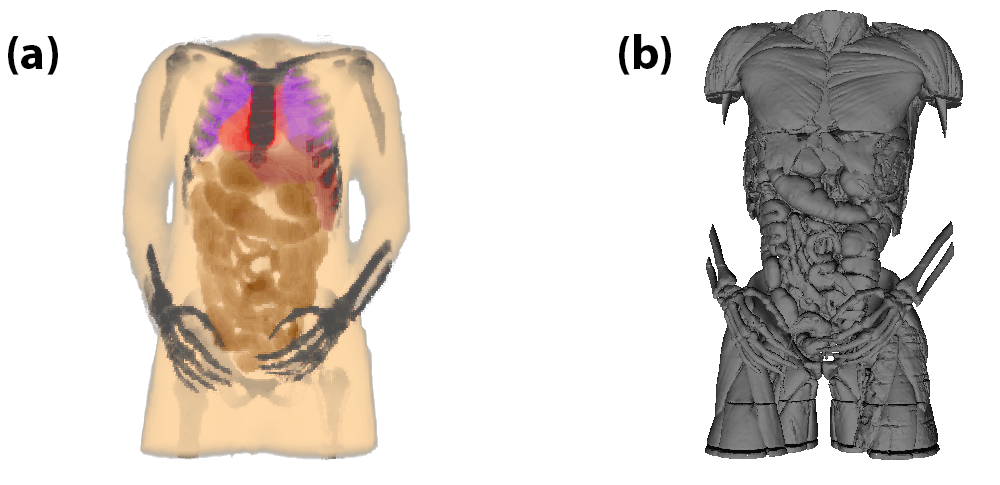
\includegraphics[width=0.9\textwidth]{IMG/volvsb-rep.png}
    \caption{La figura (a) muestra el \emph{renderizado} de la representación volumétrica del \emph{Visible Human Project} \cite{ackerman1998visible} mediante \emph{Ray-casting}. La figura (b) muestra el renderizado de la malla poligonal del mismo modelo. }
   \label{fig:HVP}
\end{figure}
%\todo{hace falta explciar la malla de tetraedros?}



Respecto a la representación de modelos anatómicos humanos, es fácil encontrar  varios modelos comerciales como pueden ser: \emph{ZygoteBody}$^{TM}$ \cite{kelc2012zygote}, \emph{Anatomium} \cite{Anatomium}, \emph{BioDigital Human} \cite{qualter2012biodigital} o modelos como \emph{Visible body} \cite{visible2012visible} que solo está centrado en músculos y dispone de una serie de animaciones predefinidas. Todos ellos representados como mallas de polígonos. Estos modelos han sido diseñados por artistas y representan cánones no realistas, además no reflejan fielmente la variabilidad anatómica de los pacientes a la que podría enfrentarse un médico. En ocasiones, estos modelos no están diseñados correctamente al presentar intersecciones y colisiones entre tejidos como se puede observar en el Entregable 3.2 del proyecto \ac{RASimAs} titulado \emph{Patient-Specific Dataset Library} \cite{ded3.2}.

En la actualidad, existe una línea de investigación muy activa para transferir datos de pacientes reales a modelos virtuales y de esta forma usar datos capturados a partir de diferentes técnicas de imagen médica (como \ac{TC}, \ac{IRM} o \ac{US}). La base de datos de  \emph{Visible Human Project} \cite{ackerman1998visible} y  \emph{Segmented Inner Organs} \cite{VoxelMan} basado en el anterior, representa uno de los modelos volumétricos de prueba más utilizado en la búsqueda de métodos para extraer modelos virtuales procedentes de imágenes médicas \cite{ferrante2017slice}.

Tanto los modelos comerciales como los modelos obtenidos a través de imagen médica muestran el mismo problema: los modelos anatómicos son presentados en una misma postura, que suele coincidir con la postura de adquisición. Esto hace que los datos de pacientes sean estáticos y, por consiguiente, no permiten adaptarse a la posición requerida. Algunos procedimientos médicos, como la artroscopia de rodilla o el bloqueo del nervio axilar, requieren posturas diferentes a las que se obtuvieron en el momento de la adquisición de la imagen médica. En el caso de la artroscopia, se necesita la rodilla flexionada frente a la habitual imagen capturada de la pierna extendida. En el caso del bloqueo del nervio, es necesario que el paciente se sitúe con el brazo en abducción de 90 grados respecto del tronco y el antebrazo en flexión de 90 grados en comparación a la mayoría de las imágenes médicas que son capturadas en una posición relajada. 

Es importante destacar que la mayoría de las técnicas de imagen médica no son capaces de capturar adecuadamente todos y cada uno de los tejidos del paciente. Por tanto, los métodos de registro entre imágenes médicas y modelos anatómicos tridimensionales que se presentan en \cite{ferrante2017slice} es habitual que se centren solo en tejidos concretos, como pueden ser la piel, huesos y músculos en general. 
En cuanto a las propiedades mecánicas de los tejidos, existen técnicas como la elastrografía \cite{MRIelastography} para recuperar la elasticidad o dureza de un tejido concreto. Aun así, esta técnica no permite la adquisición de la descripción mecánica de todos los tejidos.



%de registro entre imágenes médicas y modelos anatómicos tridimensionales que se presentan en \cite{ferrante2017slice} no son capaces de capturar adecuadamente todos y cada uno de los tejidos del paciente. En ocasiones solo se centran en tejidos concretos como puede ser la piel, huesos y músculos en general. Además, las técnicas actuales de imagen médica tampoco son capaces de recuperar las propiedades mecánicas de todos los tejidos, siendo esto un gran inconveniente si se requiere una descripción de todos los tejidos.

Por tanto, se necesita un método que permita a los simuladores tratar modelos virtuales sin importar la posición con la que fueron creados. % con tejidos internos, completos o incompletos, y poder adaptar su postura al procedimiento a entrenar. Se busca poder utilizar una variabilidad de modelos, con el objetivo de que los usuarios puedan entrenar con el máximo número de pacientes virtuales del que se dispongan 
Por ejemplo, se puede hacer mención al trabajo de  \emph{Dicko et al.}~\cite{Ali2013}.  En este artículo, los autores han desarrollado un método para modelar la anatomía interna de un paciente virtual, transfiriendo los tejidos internos de un modelo anatómico de referencia como \emph{ZygoteBody}$^{TM}$~\cite{kelc2012zygote} a un modelo registrado a partir de una imagen médica. Con esta técnica, es posible registrar y modelar los tejidos internos de datos obtenidos de \ac{IRM}. Este trabajo se centra solo en el proceso de registro y modelado sin detallar el proceso de animación utilizado, en el que no se mencionan como se realiza la etapa de \emph{rigging} o la de pesado, las cuales se detallarán más adelante. Además, se citan ciertos problemas con la interpretación de los tejidos adiposos.   


En la siguiente sección, se presentará una visión general de los diferentes algoritmos existentes para animar modelos tridimensionales de caracteres articulados. La animación consiste en deformar las representaciones superficiales 
%\todo{quieres que utilice el termino b-rep?. Marcos. Solo cuando quede bien}
o volumétricas por medio de modelos matemáticos. Estas técnicas se clasifican en dos grupos: aquellas que tienen en cuenta las propiedades físicas del modelo y aquellas que solo utilizan operaciones geométricas para animar el modelo. Actualmente, es habitual que los algoritmos geométricos estén orientados a aplicaciones interactivas, ofreciendo soluciones plausibles, %ser interactivos
%sacrificando precisión  
frente a los algoritmos físicos centrados en una deformación precisa. Aun así, existen algoritmos que combinan ambos enfoques para conseguir deformaciones más precisas para técnicas interactivas, o reducir el tiempo de cálculo para simular el comportamiento físico. 


\subsection{Animación esqueletal}
\label{art:animation}
\label{art:virtualskel}

La animación esqueletal es un método geométrico que se utiliza para animar un modelo articulado representado por su malla superficial, gracias a un esqueleto virtual, asociando los vértices a los huesos virtuales. %Esta técnica permite transferir el movimiento del esqueleto a la representación superficial. 
Esta técnica fue introducida por N. Magnenat Thalmann en 1988 \cite{thalmann88} y sigue siendo la técnica más utilizada debido a su sencillez y su fácil implementación en el cauce gráfico actual. A pesar de la existencia de métodos más realistas, esta técnica se usa prácticamente en todos los sistemas de animación interactivos ya que simplifica el trabajo de los artistas (el número de grados de libertad del esqueleto virtual es mucho menor al numero de grados de libertad de la representación superficial) o forma parte de algoritmos más complejos como paso previo. %Por ejemplo, se puede animar mediante captura de movimientos y cinemática inversa, entre otros.

La técnica se basa en una abstracción matemática, un esqueleto virtual, que se utiliza para definir los puntos de rotación de las \ac{joints} de los modelos. Este esqueleto se define como un conjunto de huesos virtuales jerarquizados que se encuentran conectados entre sí. La figura \ref{fig:virtualskeleton} muestra un esqueleto virtual superpuesto a un paciente virtual. Las esferas grises representan los centros de rotación de los \emph{\acs{joints}}, mientras que, los prismas representan la relación de herencia entre ellos. Estos huesos están pensados para que el artista dirija los movimientos del personaje y defina animaciones que la técnica de \emph{skinning} trasladará a la malla superficial según se define en \cite{thalmann88}. 

\begin{figure}[ht]
   \centering
    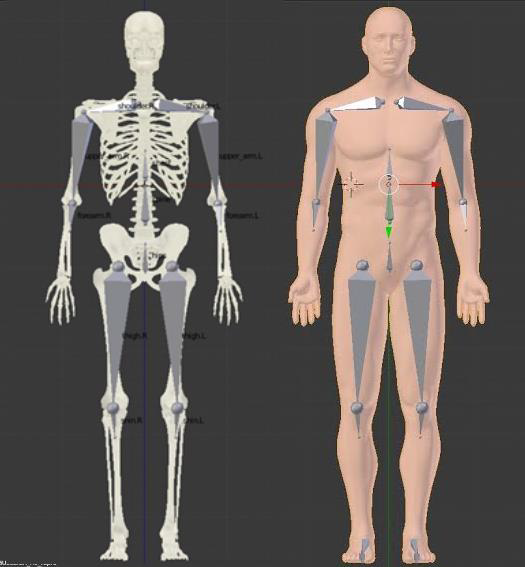
\includegraphics[width=0.8\textwidth]{IMG/virtualskeleton.png}
    \caption{Esqueleto virtual ajustado al tejido óseo de un modelo anatómico.}
   \label{fig:virtualskeleton}
\end{figure}

Con el paso del tiempo, esta técnica ha sido divida en fases que definen el cauce de la animación esqueletal:

\begin{itemize}
    \item \emph{Rigging}\footnote{Término ampliamente utilizado para la creación o adaptación del esqueleto virtual.}: en esta etapa se crea el esqueleto virtual específicamente para el modelo que se vaya a animar.
    \item Pesado: una vez creados los huesos virtuales, se asigna el peso %de influencia 
    de cada hueso para cada vértice de la piel del modelo.
    \item \emph{Skinning}\footnote{Término ampliamente utilizado para la transferencia de movimiento del esqueleto virtual al \emph{\acs{B-rep}}.}: se definen los algoritmos que van a transferir el movimiento de los huesos virtuales a la malla superficial asociada. 
    \item Selección de poses: se define la posición de los huesos que producen una deformación concreta al modelo superficial.
\end{itemize}

A continuación, se mostrará la revisión de la literatura existente para cada etapa, donde se hará especial mención a aquellas técnicas automáticas.


\subsubsection{Rigging}
\label{art:rigging}

El proceso de \emph{rigging} consiste en crear un esqueleto virtual que se adapte a la fisionomía del personaje virtual. Este trabajo normalmente es realizado por un artista ayudado de un programa de \ac{CAD} como puede ser \emph{Blender} \cite{blender} o \emph{3DS MAX} \cite{3ds}. 

Existen algunos trabajos que tratan de automatizar el proceso de creación de esqueletos virtuales siguiendo dos enfoques: generar un esqueleto virtual a partir de la \emph{\ac{B-rep}} o adaptar un esqueleto ya creado al modelo de entrada.

Algunos métodos permiten inferir un esqueleto en base a cualquier malla superficial. A partir de operaciones matemáticas (suavizado Laplaciano en el caso de \cite{laplacian}), se realiza una contracción de la malla que da lugar a un modelo alámbrico. Este será utilizado como esqueleto virtual. Este método presenta la ventaja de poder adaptarse a cualquier modelo no humanoide. Un trabajo más reciente se puede encontrar en \cite{Tagliasacchi}.

En ~\cite{borosan2012rigmesh}, \emph{Borosán et al.} presentan un método que permite modelar y crear el esqueleto virtual en el mismo instante. El artista esboza la silueta y el algoritmo genera la superficie formada por cilindros consecutivos, los cuales son utilizados para crear el esqueleto.


En otras técnicas como \cite{huang2013robust}, se adapta un esqueleto virtual predefinido al modelo de entrada. Normalmente orientado para humanoides, dividen la malla de entrada en segmentos de partes específicas de la anatomía humana (cabeza, piernas, brazos, etcétera) que se utilizan para definir los puntos de rotación de cada hueso virtual. Estas técnicas son más habituales cuando se requiere animar modelos procedentes de una nube de puntos capturados por dispositivos de captura.

En \cite{avril2016animation}, \emph{Avril et al.} se presenta un trabajo en el que, a partir de un personaje virtual de referencia, se puede adaptar el esqueleto y el pesado del modelo seleccionado a cualquier malla humanoide.


\subsubsection{Pesado}
\label{art:pesado}

Este proceso determina cual es la influencia de cada hueso virtual en cada vértice de la malla superficial.
% La consideración de esta influencia se denomina pesado, 
El cálculo de esta influencia se denomina pesado, debido a que se calculan una serie de pesos $w_{i,j}$ que relacionan un vértice $i$ con el hueso $j$.
Para asegurar una deformación correcta, se presuponen las siguientes condiciones:
\begin{eqnarray}
%\begin{equation}
\label{cond1}
w_{i,j}\geq 0 \;\;\;\;\;\;\;\; \forall i \in V \wedge \forall j \in B   \\
%\end{equation}
%\begin{equation}
\label{cond2}
\sum_{j \in B} w_{i,j} = 1\ \;\;\;\;\;\;\;\;\;\;\;\;\;\;\;\;
\forall i \in V
%\end{equation}
\end{eqnarray}
donde $V$ es el conjunto de vértices de la malla poligonal y $B$ es el conjunto de huesos en el esqueleto virtual. No puede existir un hueso que influya negativamente a un vértice, por ello se tiene que cumplir la condición \ref{cond1}. %la relacion no puede ser proporcional añ hueso ao la suma de influencia 
%Ademas, existe (se impone) una segunda condicion, 1.2, que determina la relación de pesos de todo los vertices i pertenecientes a un mismo hueso j y limita los movimientos posibles. 
Además, se debe garantizar que la suma de pesos es proporcional a las influencias de cada hueso, cumpliendo la condición \ref{cond2}.
Por último, resulta intuitivo pensar que las transiciones entre huesos virtuales deberían ser progresivas, el gradiente de los pesos debe ser suave, para evitar efectos extraños y discontinuidades en la malla.

Originalmente, al igual que la etapa anterior, un artista era el encargado de realizar la tarea manualmente, donde se utilizaban herramientas \ac{CAD} para \emph{pintar} la influencia de un hueso en la malla superficial. Actualmente en la literatura se pueden encontrar métodos totalmente automáticos \cite{huang2013robust,pan2017automatic}. 
Algunos de estos trabajos no tienen en cuenta la conectividad de la malla y puede ser que haya vértices topológicamente lejanos con pesos similares. Es por eso, que se han propuesto soluciones como \cite{Baran:2007}, donde se utiliza la ecuación del calor, suponiendo que los pesos se difunden al igual que lo haría la temperatura, permitiendo calcular transiciones más suaves en la malla. \emph{Baran y Popovi\'{c}} resuelven la ecuación en el equilibrio sobre la superficie, añadiendo transferencia de calor en los vértices más cercanos al hueso. El equilibrio en la superficie para el hueso $i$ es dado por:
\begin{equation}
\label{eqn:baran}
 \frac{\delta \mathbf{w_i}}{ \delta t} = \mathbf{ \Delta w_i} + \mathbf{H(p_i-w_i)} = 0,
\end{equation}
donde $\Delta$ es el operador \emph{laplaciano}, $p_i$ es un vector donde $p_{i,j}=1$ si el hueso i más cercano al vértice j, $p_{i,j}=0$ si no lo es, y $\mathbf{H}$ es una matriz diagonal donde $Hjj$ es la contribución del peso del hueso más cercano al vértice $j$.

Aunque esta solución es más compleja (resolución de sistemas de ecuaciones, cálculo de vecindad, etcétera), ofrece transiciones más realistas sin intervención manual. %y menor intervención manual. 
Esta técnica está restringida a mallas superficiales que deben rodear completamente al esqueleto virtual.

Existen trabajos posteriores como el de \emph{Jacobson et al.}~\cite{Jacobson:2011}, donde se mejora la etapa de pesado para ser capaz de manejar puntos de anclaje, huesos virtuales y cajas contenedoras. Se propone minimizar la energía \emph{Laplaciana} de las restricciones de los anclajes con el objetivo de conseguir una continuidad  de primer orden (Ec. \ref{eqn:1}):
\begin{equation}
\label{eqn:1}
\mathrm{arg\,min}_{\mathbf{W_j}, j=1..m}\sum_{j}^m\frac{1}{2}\int_\Omega \left \|  \nabla \mathbf{W_j}\right \|^2 dV,
\end{equation}
donde $W_j$ son los pesos del manejador $j$ y $m$ es el número de puntos de anclaje. La principal limitación es que se genera un problema disperso y cuadrático para imponer las restricciones. %No obstante, en el capítulo \ref{cap:pesado}, la solución propuesta solo requiere resolver un sistema de ecuaciones lineales.

\subsubsection{Skinning}
\label{art:skinning}

Esta etapa es la que define como se transfieren los movimientos de los huesos virtuales a los vértices que componen la malla superficial que los envuelve utilizando la ecuación de \emph{skinning}: 
\begin{equation}
\label{eqn:skinning}
\mathbf{v'_{i}} = \sum_{j \in B} w_{i,j}f(\mathbf{\theta_{j}},\mathbf{v_{i}}) 
\end{equation}
Esta ecuación determina como calcular la nueva posición del vértice $v'_{i}$ de la malla. Donde $\theta$ representa el movimiento de cada hueso $j$ que se aplica a ese vértice. %De esta forma, la nueva posición del vértice se calcula en función de la influencia del movimiento de cada hueso.

Según la formulación matemática que se desarrolle, los distintos métodos toman su nombre, como por ejemplo: \ac{LBS} \cite{thalmann88}, \ac{DQS} \cite{Kavan2008} o \ac{SBS} \cite{Kavan:2005}.



La técnica más habitual es \ac{LBS} presentada en \cite{thalmann88}, que se basa en calcular la nueva posición interpolando linealmente las matrices de transformación $T$ de cada hueso virtual:
\begin{equation}
\label{eqn:LBS}
\mathbf{v'_{i}} = \sum_{j \in B} w_{i,j}\mathbf{T_{j}v_{i}}
\end{equation}

\ac{LBS} sufre problemas debido a que la interpolación de las rotaciones se realiza de manera lineal. Esto lleva asociado efectos no deseados como: el colapso de la malla  en rotaciones (\emph{collapsing elbows}) o en giros (\emph{candy wrapper}). En la literatura, se pueden encontrar numerosas propuestas que solventan los defectos de esta técnica \cite{rumman2016state}, aunque normalmente llevan asociadas un incremento del coste computacional, o la aparición de otros artefactos no deseados. Uno de los métodos más populares es la técnica presentada por \emph{Kavan et al.} en \cite{Kavan2008}, llamada \ac{DQS}, que solventa las limitaciones de \ac{LBS} al utilizar la interpolación de cuaterniones duales (Ec. \ref{eqn:DQS}). Además, esta técnica se caracteriza por ser computacionalmente equivalente a \ac{LBS}. Aunque \ac{DQS} funciona adecuadamente en la mayoría de los casos, en algunas situaciones ocurre que la malla se deforma en exceso. Visualmente, resulta en una ganancia de volumen significativa (\emph{joint-bulging}). 

\begin{equation}
\label{eqn:DQS}
\mathbf{v'_{i}} = (\sum_{j \in B} \mathbf{DQ_{j}}w_{i,j}) \mathbf{v_{i}}
\end{equation}

Otras soluciones se han presentado como en \emph{Lee et al.}~\cite{Lee2013}, donde se describe una técnica que se encarga de resolver los problemas de \ac{DQS} cuando se realizan escalados y cizallados, movimientos muy habituales en cine de animación pero infrecuentes en modelos anatómicos.

En trabajos más recientes, \emph{Le y Hodgins}~\cite{le2016real} presentan una técnica que calcula unos nuevos \ac{COR} para cada vértice de la malla. Este enfoque solventa el problema de \emph{joint-bulging} sin incrementar el coste computacional y no sufre del defecto \emph{candy wrapper}. El único inconveniente es la necesidad de un proceso previo para calcular todos esos nuevos centros.
%\todo{pongo el algoritmo de cor?}
% \begin{eqnarray}
% \label{eqn:COR}
% R = normalize( w_{i,1}q_{1} + w_{i,2}q_{2} + . . . + w_{i,b}q_{b})\\
% t = R_{LBS}c_{i} + t_{LBS} - Rc_{i} \\
% v'_{i} =  R_{q}v_{i} + t
% \end{eqnarray}

%\todo{pongo imágenes de comparación?}
En la figura \ref{fig:corexample} se puede observar una imagen extraída de \cite{le2016real}. En esta figura se muestra una comparativa visual entre su método \ac{COR} y las dos técnicas clásicas más conocidas en la literatura, \ac{LBS} y \ac{DQS}. En cuanto a la rotación del codo, se aprecia que la articulación se colapsa (\emph{collapsing elbows}) en el caso de \ac{LBS}. En su lugar, la técnica \ac{DQS} produce un abultamiento (\emph{joint-bulging effect}), mientras que \ac{COR} resuelve ambos defectos. Respecto a los giros, es conocido que la técnica \ac{DQS} solventa el problema \emph{candy-wrapper} de \ac{LBS}. Se puede observar en las imágenes de la derecha que la técnica \ac{COR} solventa los efectos anteriormente mencionados (\emph{collapsing elbows}, \emph{joint-bulging} y \emph{candy-wrapper}). 

\begin{figure*}[ht]%[b]%[b!ht]
  \centering
  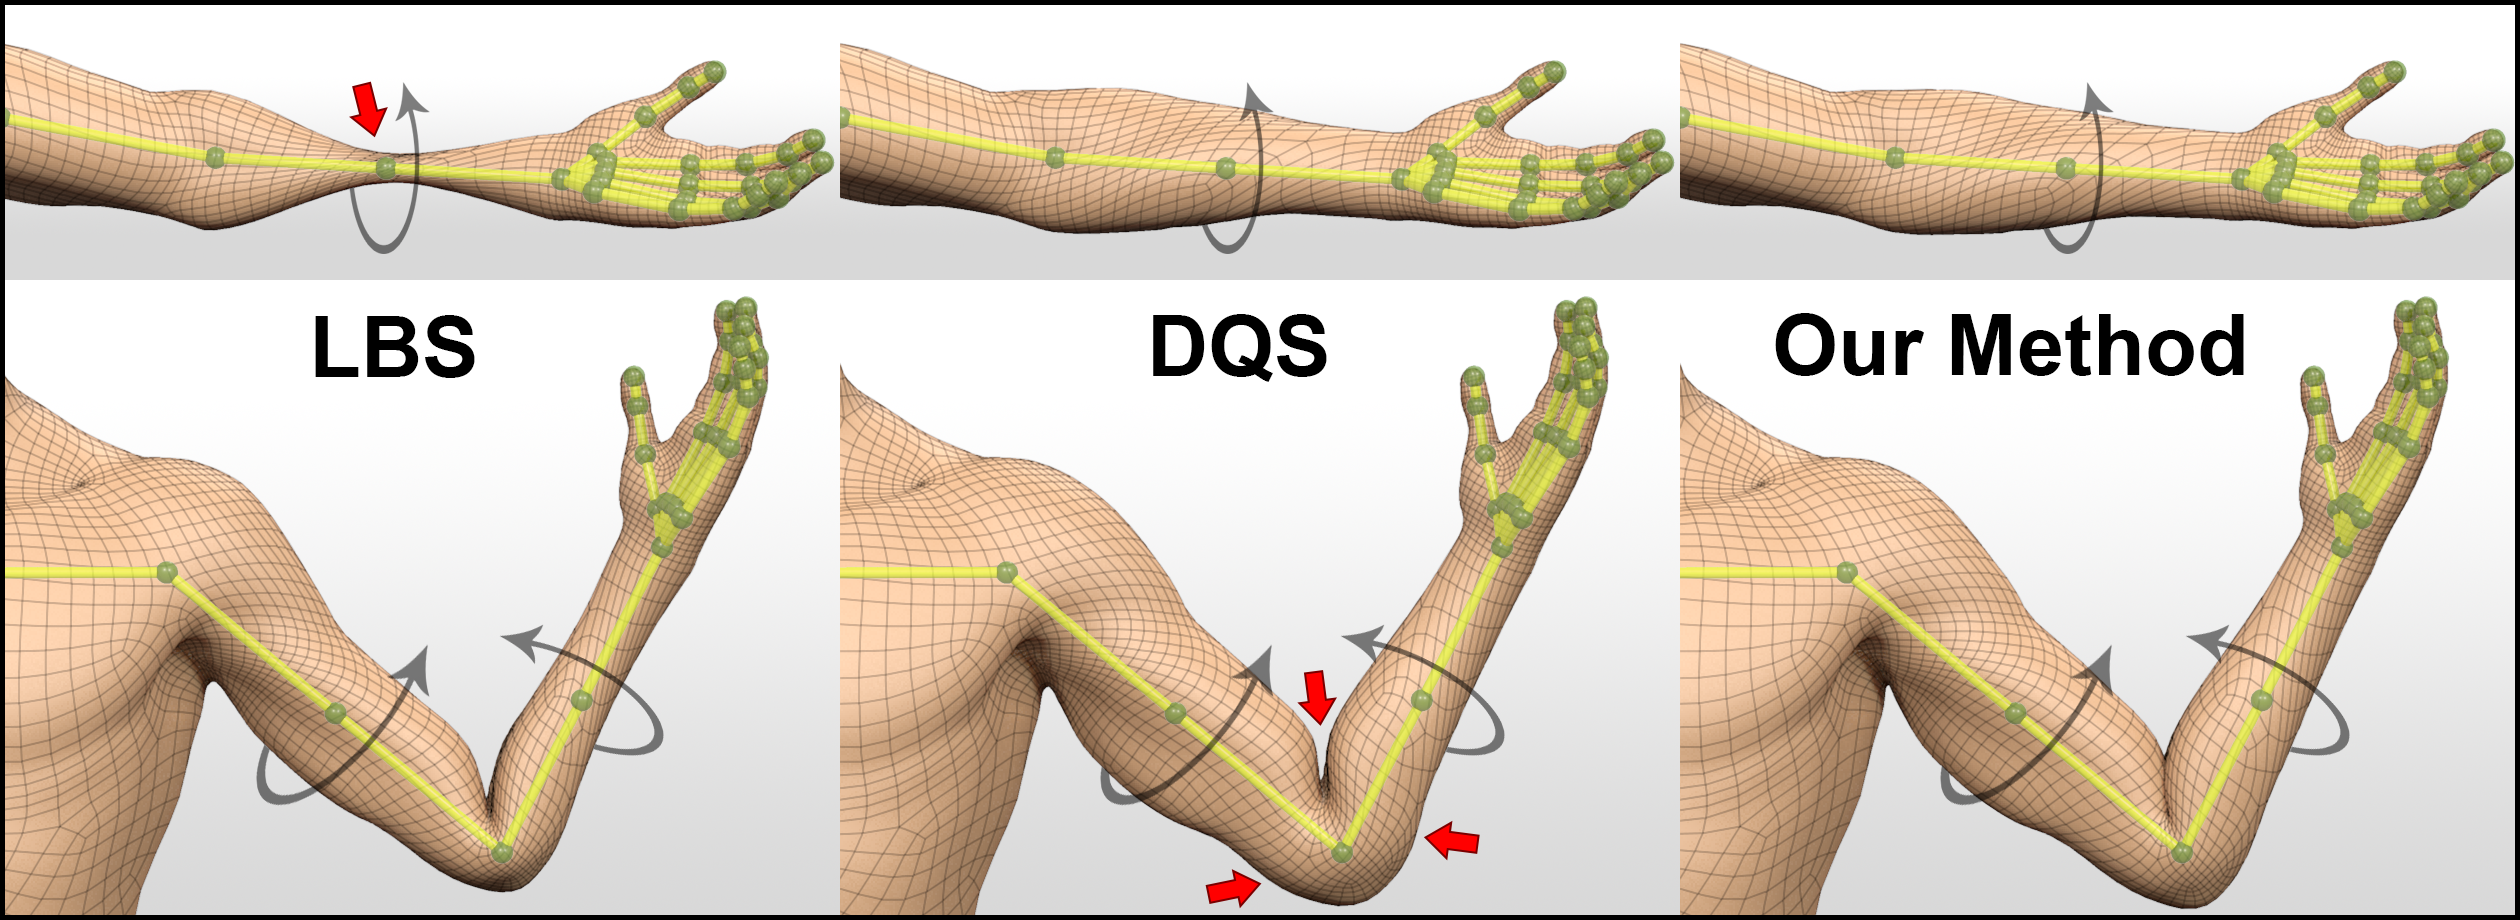
\includegraphics[width=0.90\textwidth]{IMG/corexample.png}
    \caption{En la fila de arriba, se aprecia el comportamiento de las 3 técnicas frente a los giros. \acs{LBS} sufre \emph{candy-wrapper}, mientras las otras dos técnicas no. En la fila de abajo, se puede observar la rotación del codo. En este caso, \acs{LBS} sufre \emph{collapsing elbows}, \acs{DQS} se puede apreciar el efecto \emph{joint-bulging}, y el método \acs{COR} es robusto ante estos defectos. Imagen extraída de \cite{le2016real}. }
    \label{fig:corexample}
\end{figure*}
%%%%%%%%%%%%%%%%%%%%%%%%%%%%%%%%%%%%%
%
%
Otra característica que no es habitual que se tenga en cuenta es la resolución de contactos entre vértices de la malla. En \cite{Vaillant:2014}, se propone una solución geométrica con tasas interactivas que puede solucionar las auto colisiones. \emph{Vaillant et al.} calculan un campo escalar para cada hueso, donde los vértices serán influenciados por el valor de cada campo escalar. Sin embargo, ese método no está pensado para animar modelos que representen tejidos óseos. Estructuras rígidas como los huesos se ven afectados por una función de suavizado, que se traduce en deformaciones no realistas. %16k de vertices 50 fps nosotros 1.5kk

Cuando se trata de animar modelos orgánicos, el uso de esqueletos virtuales, que solo se definen por rotaciones, presenta limitaciones al tener unos movimientos más complejos. Algunos trabajos intentan definir articulaciones basadas en modelos anatómicos \cite{joints} con \emph{splines}\footnote{Curva diferenciable definida en porciones mediante polinomios.}, mejorando así el movimiento del hueso pero dificultando la creación del esqueleto virtual y el proceso de animación.

\subsubsection{Selección de poses} 
\label{art:poses}
Esta etapa consiste en crear las animaciones  y los movimientos de los huesos virtuales que serán aplicadas a la malla superficial.   

Al igual que etapas anteriores, es habitual que estas animaciones sean creadas por artistas profesionales. Con la ayuda de las herramientas \ac{CAD}, los animadores definen el movimiento de los huesos virtuales en fotogramas clave \cite{keyframe}, al igual que se hace en la animación clásica. Una vez definidas las posiciones claves, el software calcula la interpolación de los fotogramas intermedios. Estas herramientas también incluyen algoritmos de cinemática inversa \cite{Shi:2007}, que permiten al usuario posicionar el actuador final (hueso situado en un nivel inferior de la jerarquía) y calcular la posición del resto de articulaciones superiores. 


Existen técnicas diseñadas con objeto de automatizar la fase de animación. Las técnicas de \emph{retargeting}\cite{Choi999} tienen como objetivo transferir los movimientos de un personaje virtual a cualquier otro. Trabajos más recientes no necesitan que los esqueletos virtuales tengan la misma estructura \cite{Hecker2008}, e incluso que es posible transferir movimientos entre personajes con una morfología completamente diferente \cite{Abdul2017}.


Otra técnica muy presente en los estudios cinematográficos es la \ac{MoCap}. Los movimientos realizados por un actor son capturados a través de unas balizas situadas en los trajes que se utilizan. Estos puntos característicos permiten el registro de la posición y rotación que serán trasladados al esqueleto virtual \cite{Menache:1999}. En contraste con las grandes producciones, es posible utilizar un \emph{\ac{tracker}} como Microsoft Kinect, para la animación de personajes virtuales \cite{Liu:2018}.




\subsection{Animación basada en modelos físicos}
\label{art:fisica}

Alternativamente a los métodos geométricos, los algoritmos basados en modelos físicos buscan simular el comportamiento real. Desde el trabajo de \emph{Terzopoulos et al.} \cite{terzopoulos1987elastically}, la simulación física ha tomado una enorme importancia para crear  efectos complejos (elasticidad de la piel, colisiones, vibraciones del tejido graso, el comportamiento de los músculos, etcétera) con el objetivo de generar animaciones que puedan ser usadas en cine, simuladores médicos o para el estudio de la biomecánica. 

Inicialmente, se utilizaban métodos basados en la ley de elasticidad de \emph{Hooke} como se puede ver en los trabajos \cite{russell93,wilhelms1995modeling}, pero en la última década, han ido surgiendo cada vez más modelos biomecánicos y músculo-esqueléticos. Algunos de los modelos biomecánicos son creados manualmente para una parte específica de la anatomía humana ~\cite{Lee2009}. \emph{Patterson et al.} \cite{Patterson2012} consiguen simular el comportamiento muscular pero su técnica requiere de una etapa manual larga y tediosa, normalmente realizada por un experto. De manera similar, \emph{Fan et al.}~ \cite{Fan2014} describe una técnica capaz de simular el músculo preservando su volumen. El modelo anatómico puede ser generado a partir de imágenes médicas siempre y cuando se capture el músculo en posición relajada y en su pose final. 

Aunque se pueden encontrar técnicas que recuperan los modelos músculo-esqueléticos de imágenes médicas \cite{blemker2007, gilles2010, schmid2009}, estos no suelen ejecutarse con tasa de refresco interactivo% tiempos interactivos
, siendo necesario también disponer de las propiedades mecánicas. Esta información no siempre se encuentra disponible. Hay que destacar que las técnicas citadas solo se centran en la simulación de los músculos y esqueleto, sin tomar en consideración otro tipo de tejidos.

Se pueden encontrar artículos que combinan métodos kinemáticos y dinámicos con el objetivo de conseguir tasas interactivas.  \emph{Ichim et al.} \cite{Ichim:2016} utilizan animaciones precalculadas (\emph{blendshapes}) en el contexto de animación facial. Las \emph{blendshapes} permiten un control directo y eficiente mientras que el modelo basado en físicas proporciona respuestas ante colisiones, tratamiento de la incompresibilidad y otros efectos dinámicos y colaterales. Lamentablemente, no es adecuado para la animación de personajes ya que se centra en la animación facial. 


\emph{Kadlecek et al.}~\cite{kadlecek-16-reconstructing} presentan un método para crear modelos anatómicos listos para ser usados con algoritmos basados en físicas. A partir del trabajo de \emph{Dicko et al.} \cite{Ali2013} proponen un cauce automático de reconstrucción a través de múltiples capturas preservando la estructura ósea. Aun así, en ciertas ocasiones, los autores observaron que algunos huesos sobresalían entre los músculos. Se debe remarcar que, aunque esta técnica permite simular inercias y movimientos colaterales, este trabajo no permite tasas interactivas.   % En comparación con nuestro método, utilizan tetraedros que contienen más de un tejido, mientras en el algoritmo propuesto los tejidos óseos generan sus propios tetraedros que sirven de condición de contorno en el calculo de la etapa de pesado.

\emph{Rumman and Fratarcangeli}~\cite{abu2015position} han propuesto un método inspirado en el algoritmo de deformación basado en el cálculo de las posiciones, omitiendo la velocidad y la aceleración (Point-Based Dynamics \cite{Bender:2014}). Este trabajo permite animar cualquier personaje articulado gracias a la discretización del interior del modelo, permitiendo también animar los tejidos internos. Sin embargo, el alto coste computacional requiere de mallas en baja resolución para su ejecución con tasas de refresco asumibles en entornos interactivos.% tiempos interactivos.

%se podría hablar de métodos basados en ejemplos 
%tengo un par de surveys donde podría sacar más paper

%%%% Posing
\chapter{Posicionamiento de pacientes virtuales} 
\label{cap:posing}

En este capítulo, se propone un método que permita adaptar la anatomía, interna y/o externa de un modelo anatómico virtual a cualquier pose requerida. Tal y como se explica en la capítulo \ref{cap:intro} de introducción, esta tesis se ha desarrollado en el contexto del proyecto \ac{RASimAs}, financiado por el 7º programa marco de la Unión Europea. Uno de los principales objetivos del proyecto era crear un simulador de anestesia regional que permitiese entrenar a los futuros médicos.
Este simulador debía ofrecer una amplia base de pacientes virtuales, de forma que el anestesista se pudiese enfrentar a una gran diversidad de variedades anatómicas durante su aprendizaje. Dependiendo del nervio que se desee bloquear, el procedimiento requiere una pose específica del paciente. Los algoritmos, que aquí se describen, se diseñaron para adaptar los modelos anatómicos de la base de datos de pacientes a las poses requeridas en las distintas versiones del procedimiento. Dada su importancia, \ac{RASimAs} dedicó una tarea completa a solucionar este problema (ver sección \ref{art:rasimas}). 
De esta forma, los requisitos que guiaron su diseño vinieron impuestos por las necesidades del proyecto (ver sección \ref{posing:req}). Todos los algoritmos propuestos se integraron en la herramienta \ac{TPTVPH}, desarrollada completamente en el contexto de esta tesis y que formaba parte de la \emph{suite}\footnote{Paquete de aplicaciones desarrolladas con distintos objetivos y capaces de cooperar entre sí.} de aplicaciones \ac{ITGVPH}, módulo de creación de pacientes virtuales de  \ac{RASimAs}.

%\del{Como se puede leer en el capítulo de introducción \ref{cap:intro}, el objetivo de esta tesis viene influenciado por el proyecto europeo \ac{RASimAs} cuya finalidad de crear un simulador de anestesia que pueda entrenar con una base de datos de pacientes virtuales consiguiendo variabilidad anatómica adecuada para practicar el procedimiento.
%El proyecto europeo dedica una tarea completa a solucionar la problemática de poder reposicionar modelos anatómicos con el objetivo de crear una base de datos con una gran variabilidad anatómica (ver sección \ref{art:rasimas}).}

%\todo{No está mal escrito, pero es redundante con los objetivos de RASimAs}
%\del{En el contexto de entrenamiento médico, es fundamental que los usuarios se enfrenten a la mayor cantidad de situaciones posibles. 
%Es por ello, que se ha propuesto un método que permita la creación de un conjunto de datos extenso de forma automática o semi-automática y a la vez pueda ser utilizada en cualquier simulador de realidad virtual.}

El conjunto de algoritmos que se han diseñado a lo largo de este trabajo de tesis, extienden la animación esqueletal clásica a la animación de los tejidos internos de un modelo virtual. Al tratarse de un método puramente geométrico ofrece, con un coste computacional bajo, resultados plausibles y estables. Otro de los motivos principales por los que se escogió un método geométrico frente a un método basado en modelos físicos, es la posibilidad de manipular modelos anatómicos incompletos o de los que no se dispone de sus propiedades mecánicas. Estas características, hacen que su uso sea adecuado en otras aplicaciones, incluso más allá del ámbito médico.  En el mundo del ocio interactivo, especialmente en el sector de los videojuegos, un bajo coste computacional, la estabilidad, la plausibilidad de los resultados y la posibilidad de aplicarlo a estructuras anatómicas incompletas, son características más importantes que la precisión física de las transformaciones. 

%\todo{hay que dar mas peso a lo de los modelos incompletos que a la interactividad. En el caso de rasimas es más importante. }
%\del{ Con este propósito, se han diseñado y adaptado diferentes algoritmos de animación esqueletal con el objetivo de animar tejidos internos y externos de un paciente virtual. Se ha elegido utilizar métodos geométricos que permiten la creación de resultados plausibles y a la vez tienen la ventaja de que permiten una deformación interactiva. Esta ventaja frente a los métodos basados en físicos dan lugar a que el algoritmo presentado en este capítulo pueda incluirse en cualquier simulador que requiera de deformación en tiempo real. Otra ventaja que tiene el método propuesto es la posibilidad de manipular modelos anatómicos incompletos o que no se disponen de sus propiedades mecánicas.}

\section{Requisitos de diseño}
\label{posing:req}
%\new{Decisiones de diseño}

%\todo{De manera ideal no son los requisitos nos los fijan los socios. Sino los objetivos del proyecto. Lo cambiamos a decisiones? }
%\del{Al formar parte de un proyecto donde intervienen más grupos de investigación, la tarea específica viene acompañada de una serie de requisitos que necesitan ser respetados, pero al mismo tiempo es la principal motivación que se encuentra al formular una solución innovadora:}
En las etapas iniciales del proyecto \ac{RASimAs} se establecieron los objetivos del módulo de creación de pacientes virtuales \ac{ITGVPH}, del que la herramienta \ac{TPTVPH} formaba parte. A partir de dichos objetivos se definieron los requisitos y, por ende, de los algoritmos que lo componen.


%\todo {0.No está escrito como unos requisitos. Mezclas requisitos con decisiones de diseño!!!
%1. El enfoque geométrico no es una recomendación es una consecuencia de los objetivos
%2. Realmente en el estado del arte, se ha demostrado que el enfoque geométrico es menos sensible a la calidad de datos de entrada?????. 
%3. a que te refieres con tipos de datos. Realmente te refieres a modelos incompletos. }
\begin{itemize}
    \item El proceso de selección de poses debe ser guiado y supervisado por un experto para garantizar la validez de los modelos generados. Dado el coste económico del tiempo de un experto, la herramienta debe tener una interfaz sencilla y los algoritmos deben ejecutarse en modelos complejos con tasas de refresco interactivas.
    \item La intervención del usuario se limita a la selección de la pose final. El resto de procesos involucrados en la preparación de los modelos deben realizarse de forma automática.
    \item Los datos de entrada se obtienen promediando datos de diferentes pacientes reales y registrándolos sobre el modelo de \emph{ZygoteBody}$^{TM}$ \cite{kelc2012zygote}. Los datos de pacientes reales provienen de distintas técnicas de imagen médica (\ac{US}, \ac{IRM}, \ac{TC}). Dado que no existe ninguna técnica de imagen capaz de capturar todas las estructuras anatómicas internas, los pacientes virtuales generados no disponen de modelos de todos sus tejidos internos. Solo se garantiza que se cuenta con los modelos adecuados de la piel y los huesos. 
    \item En el momento de realizar el posicionamiento del paciente virtual, no se conocen las propiedades mecánicas de las distintas estructuras anatómicas que lo componen.
    % \todo{Te lo he rescrito porque creo que me suena raro. Creo que no resaltas lo que es realmente importante. Aaron: Me gustaba lo de generar colisiones adicionales... }
     %\del{Para mantener la calidad del modelo anatómico de las siguientes etapas y tareas dependientes de esta (p. ej. el módulo de \ac{US}), el resultado de este algoritmo no deberá generar colisiones adicionales indeseables entre los tejidos y tener igual o menos colisiones que las existentes al llegar como entrada.}
    \item Los algoritmos propuestos deben evitar que se produzcan autocolisiones o colisiones entre los distintos tejidos, dado que esto podría provocar fallos en  algunos módulos del simulador. El módulo de \ac{US} de \ac{RASim} es especialmente sensible a estos artefactos.
     %\item \del{Se recomienda un enfoque geométrico ya que, en fases previas al proyecto, se consideró la posibilidad de utilizar un método basado en físicas para la tarea en cuestión. Como se ha podido comprobar en el estado del arte \ref{art:animation}, un enfoque geométrico es menos dependiente de la calidad de los datos de entrada, obtenidos por etapas anteriores en este proyecto. Un modelo basado en físicas necesitaría una descripción completa de todos los tejidos; sin embargo, el método geométrico puede ser útil si estos datos no están disponibles.}
    %\item  \del{\ac{TPTVPH} (ver sección \ref{art:rasimas}) podrá ser capaz de trabajar con cualquier tipo de datos que procedan de un paciente virtual. Como no se puede asegurar que todos los tejidos se encuentren disponibles, el algoritmo deberá ser lo máximo flexible posible para manejarlos.}
    
    %\item \todo{He usado este objetiv para meter la importancia de la interactividad.}\del{Aun así, el proceso de posicionamiento tendrá que ser supervisado. Profesionales cualificados definirán un conjunto genérico de posturas para el procedimiento de \ac{RA}. Un método semiautomático será desarrollado para facilitar la consecución de la validez y calidad de los modelos de pacientes virtuales.}
    %\item \del{El usuario podrá modificar la postura del \ac{VPH} a través de una interfaz 3D interactiva \del{con la intención de reducir el procedimiento completo}. El algoritmo deberá ejecutar en tiempo real para mejorar la experiencia de uso. }
    
 \end{itemize}


%\todo{No puede haber solo una subsección!!!}
%\subsection{Requisitos del posicionador de pacientes virtuales}

%\todo{Si te sobra tiempo, puede describir las ventajas de los métodos fiscos sobre los geométricos. Coste computacional, estabilidad, flexibilidad. Por otro lado, los cambios de poses requieren grandes movimientos que para ser capturados de forma precisa necesitan que se tengan en cuenta numerosos comportamientos que no fáciles de simular (deformaciones elásticas, interacciones:  deslizamientos, contactos). Requieren modelos completos y bien caracterizados... }

En un primer momento, se planteó la posibilidad de trabajar con técnicas basadas en modelos físicos en aras de conseguir una deformación precisa de los tejidos. Esta opción fue desechada principalmente por no disponer de una descripción mecánica de los tejidos involucrados en la simulación. Estás técnicas generalmente requieren importantes recursos computacionales lo que impide que puedan usarse en aplicaciones interactivas. El problema se agrava cuando se quieren simular grandes deformaciones que involucran diversos y complejos fenómenos físicos.

Por otro lado, muchas veces la resolución de los sistemas de ecuaciones diferenciales que modelan el comportamiento del sistema requiere de métodos numéricos que no siempre son estables. En experimentos iniciales, se optó por trabajar con técnicas muy utilizadas como las propuestas en  \cite{Muller2004} e implementadas en \ac{SOFA}. Pronto quedó patente que los modelos de tejidos utilizados eran demasiado complejos como para que este tipo de técnicas funcionasen de forma adecuada.
%\del{Como se puede leer en la sección \ref{art:animation}, estos métodos basaban sus resultados en un alto coste computacional, o en centrarse en una única anatomía.  Además, algunas técnicas requieren de modelos muy bien caracterizados o de capturas en diferentes posiciones, lo cual es el principal objetivo que quiere solventar la herramienta planteada. Técnicas clásicas como \cite{Muller2004}, se ejecutaron en el software de simulación \ac{SOFA}. Los modelos iniciales del sistema eran demasiado complejos para conseguir tasas de refresco adecuadas para una interacción con el usuario.}
Durante el desarrollo de esta tesis, se han propuesto nuevas técnicas que podrían cumplir con algunos de los requisitos planteados (ver sección \ref{art:fisica}). En \cite{abu2015position}, se propone un método capaz de simular el comportamiento interno de la anatomía, permitiendo la caracterización mecánica de los tetraedros según el tejido anatómico al que pertenecen.  
%\del{con el objetivo de generar movimientos de los tejidos óseos plausibles}
%\todo{No entiendo que quiere decir: -- se puede asignar propiedades mecánicas diferenteas a cada tetraedro.}. 
El principal inconveniente de esta técnica es la imposibilidad de conseguir tiempos interactivos con la complejidad de los modelos anatómicos que se estaban utilizando. Además, la publicación de este artículo ha sido posterior a la fecha de incorporación del algoritmo en el proyecto europeo.
%\todo{Yo reescribiria la última frase es muy enrevesada}\del{, además de tener en cuenta que su aparición fue posterior a la fecha de finalización de la tarea.}

Como consecuencia de lo expuesto, se decidió desechar la opción de trabajar con métodos basados en modelos físicos y se optó por diseñar una técnica geométrica. En las siguientes secciones se describirá el método propuesto.
%%%%%%%%%%%%%%%%%%%%%%%%%%%%%%%%%%%%%%%%%%%%%%%%%%%%%%%%%
\section{Algoritmo propuesto}
\label{posing:method}
%%%%%%%%%%%%%%%%%%%%%%%%%%%%%%%%%%%%%%%%%%%%%%%%%%%%%%%%%
%\todo{1. Indicar muy brevemente las ventajas de la animación esqueletal alineadas con los objetivos. 2. Indicar porque la técnica clásica no se puede utilizar. La extendemos para anatomía interna. 3. No usamos las técnicas clásicas porque no tiene en cueta la anatomía interna. %2. No entiendo la seguna parte de la frase}
En este apartado, se proponen un conjunto de técnicas capaces de animar la anatomía interna y externa de un paciente virtual. El cauce de animación, que aquí se describe, fue diseñado para trabajar con \emph{\acs{B-rep}s} de los distintos tejidos, aunque dada la flexibilidad del enfoque planteado, posteriormente se extendió a otro tipo de representaciones (ver sec. \ref{posing:animvol}). 
%\todo{
%mete la referencia. Lo he contado por que tú lo haces pero no se si es el mejor sito. 
%Tienes que ir soltando las ideas una a una, no todas a la vez. }
%
%\del{El objetivo es ser capaz de modificar toda la anatomía interna y externa de un modelo anatómico virtual usando una representación superficial. En el mundo de los gráficos por computador, tradicionalmente, se ha utilizado la animación esqueletal para \new{animar modelos articulados}. ????????????????????????????????? Aunque permite una animación de modelos complejos en tiempo interactivo, no tiene en cuenta la relación espacial entre tejidos. Por esta razón, se ha diseñado un cauce basado en la animación esqueletal que se extiende para el uso de representaciones volumétricas.????}
%\todo{%Lo reescribo yo!. Todo esto es muy confuso. 
%No hay un hilo conductor ni una idea clara que vender} 

En el mundo de los gráficos por computador, tradicionalmente se ha utilizado la animación esqueletal para animar modelos articulados, dado que produce resultados visualmente plausibles y son muy eficientes desde el punto de vista computacional. Este conjunto de técnicas se basan en asignar un esqueleto virtual a la representación poligonal de la superficie de un modelo 3D. Es conveniente destacar que un esqueleto virtual no es más que un conjunto jerárquico de huesos virtuales donde los puntos de rotación de cada hueso se definen localmente en el sistema de referencia del padre. 
La idea que subyace bajo esta aproximación es que el número de grados de libertad del esqueleto virtual es muy inferior al número de grados de libertad de la malla superficial. Este tipo de técnicas no pueden aplicarse directamente al problema que se ha enunciado en la sección anterior, puesto que el proceso de animación requiere de la intervención de uno o varios artistas en la preparación de los datos. El resultado final dependerá en gran medida de las destrezas de los artistas implicados en el proceso. 

Tal y como se comenta en la sección \ref{art:animation}, en la bibliografía existen distintas técnicas que buscan automatizar algunas de las etapas de este cauce, pero no están diseñadas para lidiar con modelos que contengan estructuras anatómicas internas. Por consiguiente, en este trabajo de tesis, se propone cómo adaptar el cauce de la animación esqueletal clásica de forma que se pueda aplicar a modelos anatómicos de forma automática. 
%\del{En lugar de utilizar las técnicas clásicas de animación esqueletal, se ha propuesto una nueva manera novedosa de animar anatomías de personajes de manera eficiente, ya que para animar todos los tejidos de forma separada implicaría que habría que realizar las etapas de la animación para cada tejido de manera independiente y que no se podría asegurar que se generaran auto colisiones entre ellos.}

La idea principal que hay detrás del algoritmo propuesto es calcular un campo de desplazamientos continuo a partir del movimiento de los huesos
%\todo{si no es continuo todo lo que dices a continuación no sirve}
en el interior del paciente virtual y utilizarlo para transformar sus estructuras internas. Esto permite deformar los tejidos de forma independiente y, aun así, garantizar que estos se muevan solidariamente, asegurando que no se produzcan colisiones y/o autocolisines, siempre y cuando estos estén muestreados con la suficiente resolución. 
%\del{ solidaria sin necesidad de realizar cálculos independientes y asegurar de esta manera que no se producirá nuevas colisiones.} 
%\todo{cuentalo luego}\del{Además, esta forma de trabajar permite no sólo animar representaciones superficiales, sino que es factible animar modelos volumétricos.}
%\todo{Relata la idea principal. Crear el despalazamiento a partir del movimiento de los huesos. 2. Expliar la diferencia enter hueso virtual y tejido oseo. 3. Una vez acabado el parrafo lee toda esta into para que no haya cosas duplicadas. }
%
De cara a calcular el citado campo de desplazamientos a partir del movimiento del tejido óseo, se discretizará el interior del paciente mediante una malla \emph{Lagrangiana}\footnote{Los marcos de referencia \emph{Lagrangianos} formulan el problema en el sistema de referencia del objeto frente a los \emph{Eulerianos} que formulan el problema en función de una base fija del espacio.}. Después, se calculará la influencia de cada hueso sobre el movimiento de los vértices de la malla \emph{Lagrangiana} y  se utilizará para transformar las representaciones superficiales de los distintos tejidos. 
%\del{La deformación del campo de desplazamientos vendrá dada por el movimiento del tejido óseo. La influencia de uno o un grupo de huesos reales definirá el movimiento del campo y en consecuencia, el del resto de los tejidos mapeados con la representación volumétrica generada a partir de la piel. }
%\todo{Aaron cuida más la redacción. O me pasas cosas más trabajadas o no vamos a acabar nunca!!!.}

Al igual que en la animación esqueletal clásica, esta técnica requiere construir un esqueleto virtual en el que definir las transformaciones que se aplicarán al modelo articulado. Destacar que en el caso que aquí se presenta, esta estructura puede calcularse a partir del tejido óseo del paciente virtual.
%\del{El movimiento del tejido óseo será dirigido por los huesos virtuales. Estos serán creados y ajustados teniendo en cuenta la anatomía real del paciente virtual, construyendo un esqueleto virtual específico. }


%\todo{1. todo automático menos la selección de la pose. 2. Indicar que la animación tradicional confía en el artista en muchos paso. Marcos 2: Este párrafo no explica lo que te pedía. Eso esta explicado antes. Si quieres hablar de la animación hazlo en el paso correspondiente. Pero reescribe este parrafo no esta muy bien. }


Por último, se permitirá al usuario seleccionar la pose del paciente virtual de forma interactiva. Dentro del contexto de esta tesis, el objetivo es permitir que un profesional médico supervise la correcta deformación de los tejidos, con la finalidad de conseguir posiciones útiles para el entrenamiento. Por otra parte, se podrán almacenar posturas predefinidas para automatizar el proceso para futuros modelos anatómicos.


%\del{En la industria, es el animador el que se encarga exclusivamente de los movimientos de los personajes, confiando en sus habilidades???????? """"y del rigging y del pesado""""!!!!!!!!. Otro de los objetivos propuestos para este algoritmo es permitir a un médico dirija y supervise la deformación del paciente virtual de manera interactiva. A su vez, puede guardar posturas interesantes que permitan animar los modelos automáticamente en un futuro.
%Se ha buscado en la bibliografía aquellas técnicas automáticas que puedan ser útiles como se puede leer en el estado del arte (sec. \ref{art:anatomy}) y se han adaptado para ser incorporadas en este método con el objetivo de reducir la interacción del usuario a la selección de pose.""Me cuesta enteder que idea quieres trasmitir""} 
%o dejará la elección de la postura a un profesional médico que supervise la correcta deformación de los tejidos de forma interactiva.


%Como se ha especificado en la sección \ref{posing:req}, esta técnica ha sido diseñada para funcionar con anatomías incompletas siendo sólo obligatorio que la piel y los huesos estén correctamente identificados. \todo{1. Esta frase no se como se enlaza con la anterior. 2. repites la idea de etapas automaticas que ya habías explicado en el paso anterior.}\todo{aqui te quedaste}%El algoritmo propuesto sigue la línea del cauce clásico de animación esqueletal, modificando aquellas etapas con el objetivo de que sea automático y permita modelos incompletos.

%\del{Por tanto, el algoritmo propuestose puede dividir en las siguientes etapas}. 
A continuación, se detallan las etapas en las que se divide el algoritmo (ver Fig. \ref{fig:Resumen}). Tal y como puede comprobarse, muchas de las etapas se inspiran en la animación esqueletal tradicional:
%\todo{Déjalo en ingles, pero en el estado del arte, cuando se hable de rigging, mete un nota al pie donde digas lo que es. Hecho }
\begin{itemize}

	\item \emph{Rigging}: %\todo{Se que has traducido del ingles, pero tio!!! que tu hablas castellano} \del{Un esqueleto virtual predefinido \del{es} ajustado a la anatomía del personaje.}
	en la primera etapa, se adapta un esqueleto virtual a la anatomía del paciente virtual. El algoritmo usa el tejido óseo para calcular el centro de rotación de cada articulación del hueso virtual.
	
     \item \emph{Volumetrización}: en esta etapa, se genera una malla de tetraedros que volumetriza el interior del modelo. Esta malla se genera a partir de la piel y los huesos del paciente virtual y sirve para definir un campo de desplazamientos continuo, que se asociará con el movimiento de los huesos.

    \item \emph{Pesado}: a continuación, se calcula de manera automática la influencia del tejido óseo sobre cada vértice de la malla de tetraedros. 
    
    \item \emph{Mapeado}: se asignan los tejidos a los tetraedros de la malla volumétrica. 

    \item \emph{Selección de pose}: en esta etapa, el movimiento de los huesos virtuales es transferido a la malla de tetraedros, usando una técnica estándar de \emph{skinning}: \ac{LBS}, \ac{DQS} o \ac{COR}. 
    Después, el movimiento de estos tetraedros se transferirá a los vértices de los tejidos del paciente virtual.
    %\del{aplicado a los tejidos del resto del modelo}\todo{Hay algo raro}. 
    Esta etapa puede ser interactiva, dejando al usuario elegir la pose, o pueden usarse otras técnicas de animación (p.ej. \ac{MoCap}) con el objetivo de que la etapa se ejecute de manera automática.%\todo{La cinemática inversa no es automática, es interactiva. }
    \item \emph{Optimización}: de forma opcional, el usuario podrá refinar el resultado obtenido utilizando un método que preserva el volumen del modelo anatómico.
\end{itemize}

%\todo{rehacer imagen resumen}
%\todo{hazla más grande}
\begin{figure*}[!th]
   \centering
    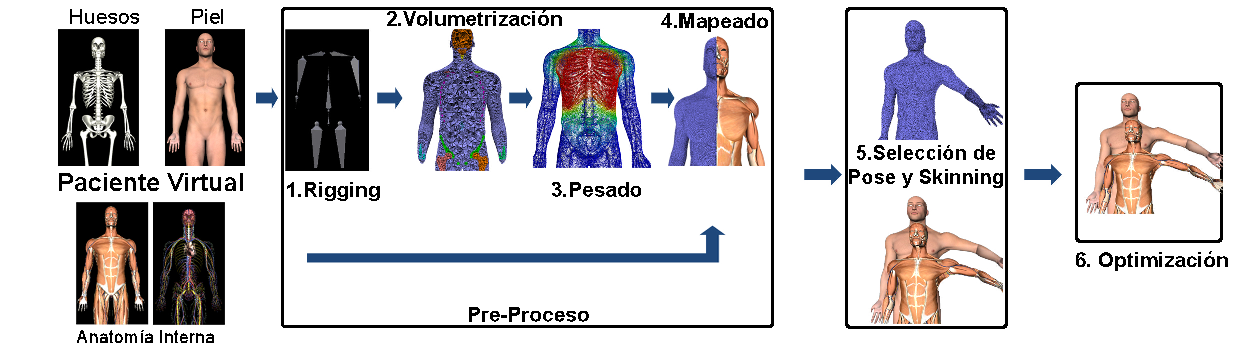
\includegraphics[width=\textwidth]{IMG/resumen.pdf}%[width=0.95\textwidth]
    \caption{Perspectiva general del algoritmo propuesto.}
		\label{fig:Resumen}
\end{figure*}


%

A continuación, se describirá detalladamente cada una de las etapas por separado, remarcando aquellas innovaciones y adaptaciones hechas específicamente en el contexto de este trabajo.



%%%%%%%%%%%%%%%%%%%%%%%%%%%%%%%%%%%%%%%%%%%%%%%%%%%%%%
\subsection{Rigging}
\label{posing:rigging}
%%%%%%%%%%%%%%%%%%%%%%%%%%%%%%%%%%%%%%%%%%%%%%%%%%%%%%
De manera similar a los huesos reales, un esqueleto virtual permite el movimiento del personaje que se quiere animar. El esqueleto virtual está formado por un conjunto jerarquizado de huesos y su posición en reposo se define a partir del sistema de referencia del hueso padre. De esta forma, la transformación que se aplica a cada vértice se expresa localmente en el sistema del coordenadas del hueso al que está asignado.  % \del{Este movimiento puede ser fácilmente ampliable a otros tipos de movimientos más complejos discutidos en la sección \ref{art:rigging}}. 


%\del{De la misma manera, se han mencionado varias formas de crear o ajustar un esqueleto virtual a un modelo de entrada.}

En la bibliografía pueden encontrarse distintas técnicas que permiten automatizar la creación del esqueleto virtual (ver sec. \ref{art:rigging}). Lamentablemente, la mayoría de ellas requieren que el esqueleto virtual esté completamente contenido en los modelos que se desean animar. En el sistema propuesto, todos los pacientes virtuales provienen de registrar un paciente tipo utilizando un modelo de referencia.  De esta forma, se creará un esqueleto virtual tipo y será el algoritmo de registro el encargado de adaptarlo a cada paciente.  %\del{se ha optado por crear un procedimiento por el cual se ajusta un esqueleto virtual predefinido al tejido óseo del paciente virtual. Se utiliza la propia representación superficial del tejido para definir un centro de rotación y los %\todo{muy muy confuso.}
%\todo{
%1. Explica que en la bibliografia existen técnicas que crean en el esqueleto y otras que ajustan uno existente. 
%2. En Rasimas los pacientes se generan registrando datos reales en el modelo del Zygote. 
%3. Redacta lo que viene a  continuación para que este bien ligado con esto. 
%4. Tienes que encuenta que etiquetas el modelo en reposo. %Recuerda el documento que nos pasó antoine. De hecho puedes poner este docuemento en el apendice y citarlo. 
%De verdad falta mucha información}

Con este objetivo, se han identificado manualmente en el modelo de referencia, las regiones significativas de cada hueso o conjunto de huesos, a partir del cual se calculará el sistema local de referencia del hueso virtual. En la figura \ref{fig:humero}, se pueden apreciar las distintas regiones seleccionadas para una muestra de diferentes huesos. 
Las zonas rojas sirven para calcular el centroide que se usará como punto de rotación. Con este punto y los centroides obtenidos de las áreas de color azul y verde, se pueden estimar dos vectores ortogonales: un vector vertical entre la zona roja y verde; y otro horizontal entre la zona verde y azul. El tercer eje se calcula mediante el producto vectorial de ambos. Estos vectores servirán para definir el sistema local de referencia para esa articulación. Para hacer estos cálculos más robustos, el algoritmo considerará (cuando sea posible) regiones grandes, minimizando los posibles defectos de un mal registro. Este proceso es específico para cada hueso virtual y puede ser fácilmente ampliable a otros tipos de huesos o agrupaciones de huesos. La explicación sobre qué zonas se han identificado en este sistema se podrá consultar en el apéndice \ref{anexo:rigging}. 
%
%\del{Estas zonas etiquetadas se identifican en el modelo anatómico de entrada.} 
Inicialmente, en el proyecto \ac{RASimAs}, se utilizó como modelo de referencia a  \emph{ZygoteBody}$^{TM}$, pero se puede asumir que el trabajo realizado puede extenderse a otros modelos de entada.
%\del{ de la herramienta \ac{ITGVPH}. 


Esta etapa concreta ha sido desarrollada en colaboración con el Dr. \emph{Antonie Serruier}, miembro del proyecto \ac{RASimAs} y se ha basado en anteriores trabajos \cite{QUIJANO20131703}.
%\todo{No entiendo esta idea final. Aaron: La idea de como sacar el centro de rotación esta explicada en ese paper}
%\todo{revisar los colores de las fotos}
%\todo{Aumenta el tamño de todas las imágnes}

%\todo{indica el código de colores}
\begin{figure}
   \centering
    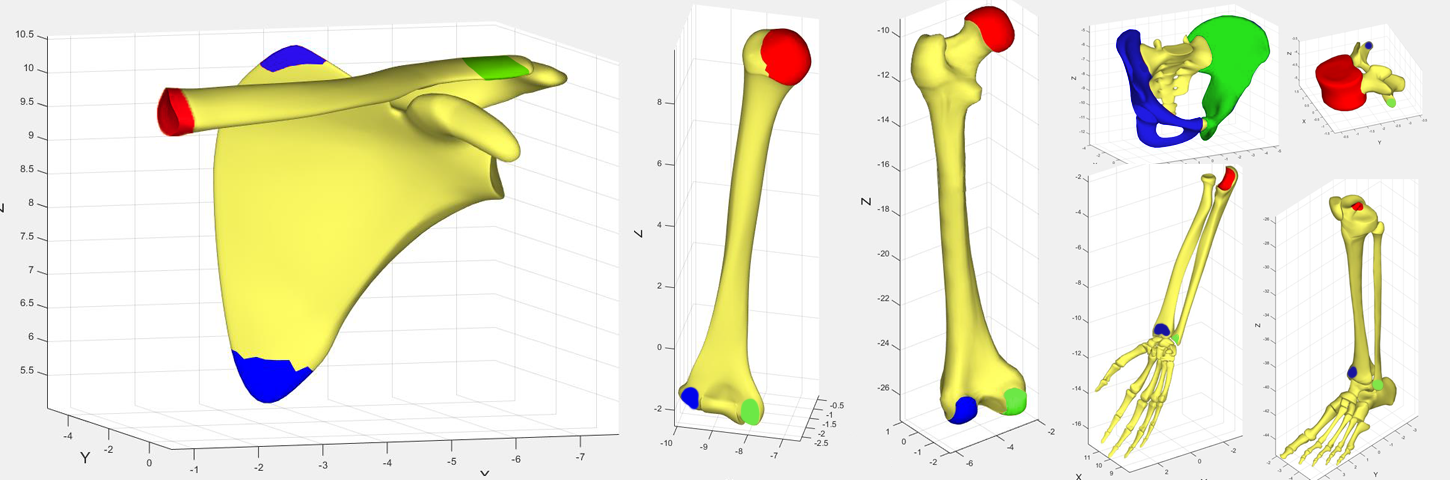
\includegraphics[width=0.95\textwidth]{IMG/rigshoulder.png}%[width=0.8\textwidth]
    \caption{La imagen muestra los huesos del modelo de referencia antes de registrar los datos del paciente. Las áreas coloreadas se utilizan para calcular el sistema de referencia de cada articulación. El centro de rotación se calcula a partir de las zonas rojas. Dos vectores ortogonales se calculan con las zonas azul y verde. El tercer vector ortogonal se calcula en base a los dos anteriores.}
\label{fig:humero}
\end{figure}


%%%%%%%%%%%%%%%%%%%%%%%%%%%%%%%%%%%%%%%%%%%%%%%%%%%%%%
\subsection{Volumetrización}
\label{posing:volumetrizacion}
%%%%%%%%%%%%%%%%%%%%%%%%%%%%%%%%%%%%%%%%%%%%%%%%%%%%%%
%
Como se ha introducido anteriormente, el objetivo es crear un campo de desplazamientos continuo que permita mover la anatomía interna del paciente virtual. El algoritmo discretiza el interior del modelo utilizando la piel y el tejido óseo como referencia, obteniendo una malla volumétrica formada por tetraedros. %\del{Esta malla de tetraedros es una pieza clave del algoritmo que se utilizará para calcular el citado campo de desplazamientos.}
La siguiente etapa (sec. \ref{posing:pesado}) calculará la influencia del movimiento de cada hueso en los vértices de los tetraedros, de forma que el movimiento de los huesos afecte a los vértices de la malla volumétrica. El campo de desplazamientos se obtendrá de forma implícita interpolando el desplazamiento de los vértices en el interior de los tetraedros, mediante el uso de coordenadas baricéntricas. %\del{Esta malla será fundamental en las siguientes etapas.}
%\del{Después, esta malla será donde se calcule el campo de desplazamiento (Sec. \ref{posing:Poses}). También, el campo de desplazamientos guiará la animación del modelo virtual gracias al cálculo del mapeado entre los tetraedros generados en esta etapa y los distintos tejidos (Sec. \ref{posing:Mapeado}).}  \todo{Estas ultimas frases son muy raras, sobretodo la final. Explicas cosas que no son necesarias para esta etapa. }


%\todo{No te das cuenta de confusa que es esta frase. Lo que quieres decir es que no calculas directamente la malla de tetraedros, primero creas una imagen volumétrica. Reescribe}
%\del{En lugar de proceder al proceso de discretización con las representaciones superficiales de los tejidos, se ha optado \new{por} generar una representación volumétrica a partir de la piel y los huesos como paso intermedio para controlar el proceso de discretización y mejorar la robustez del algoritmo. Se genera una imagen en tres dimensiones compuesta por \emph{vóxeles}\footnote{unidad cúbica mínima para representaciones volumétricas} que permitirá simplificar el etiquetado aquellos \emph{vóxeles} que \del{colisionan con} \new{pertenezcan a} la piel y los huesos.}\todo{simplificar?}
La malla volumétrica no se calcula directamente a partir de la representación superficial de los tejidos del paciente. En su lugar, se construye una imagen tridimensional en la que se etiquetan los \emph{vóxeles} que pertenecen a los huesos y la piel del paciente virtual. Este paso intermedio permite controlar el proceso de discretización y mejora su robustez.
%\del{La malla volumétrica no se realiza de forma directa, sino que se ha decidido general una representación superficial a partir de la piel y los huesos como paso intermedio para controlar el proceso de discretización y mejorar la robustez del algoritmo. Se genera una imagen en tres dimensiones compuesta por \emph{vóxeles}}\del{  que permitirá simplificar el etiquetado aquellos que pertenezcan a la piel y los huesos. }
El tamaño de la imagen 3D depende de los tamaños del \emph{vóxel} y de la caja contenedora del modelo. Cuanto más grande sea dicha caja y el tamaño del \emph{vóxel} más pequeño, más detalle tendrá la imagen 3D resultante. Un elevado número de \emph{vóxeles} implicará un mayor consumo de tiempo y memoria.
%\del{Sin embargo, hay que tener en cuenta que a más detalle, más tiempo de cálculo y más consumo de memoria será necesario.}
%\todo{sigue sin gustarme la frase. Piensala más}
Para esta tesis se ha establecido un tamaño de celda que permita tener como máximo una caja contenedora de tamaño 250x700x120 \emph{vóxeles} en todos los modelos probados.

El proceso de \emph{voxelización} comienza etiquetando aquellos \emph{vóxeles} que coinciden con la piel (fig. \ref{fig:voxelizacion}a). Después, los \emph{vóxeles} interiores se etiquetan usando la técnica descrita en \cite{SUZUKI20031} (fig. \ref{fig:voxelizacion}b).
%\todo{expresalo de otra manera}
En este punto, se ha decidido añadir una etapa en la que se eliminan los \emph{vóxeles} marcados como piel (fig. \ref{fig:voxelizacion}c). %\del{donde aquellos \emph{vóxeles} que pertenecen a la superficie de la piel vuelven a estar no etiquetados \del{como vacíos}}. 
Este paso se ha introducido para mejorar la robustez del método en zonas que podrían quedar interconectadas por su proximidad. 
%\todo{No pongas resultados pon la referencia!}
En el apartado \ref{posing:result} se mostrará como esta etapa mejora el resultado final y evita problemas importantes. Finalmente, se procede a etiquetar los \emph{vóxeles} que corresponden a cada hueso como se muestra en la imagen (fig. \ref{fig:voxelizacion}d), de forma similar al procedimiento que se siguió con la piel. 
%
%\todo{puedes hacer la imagenes más grandes. No hay limite de espacio!}
%
\begin{figure}[th]
   \centering
    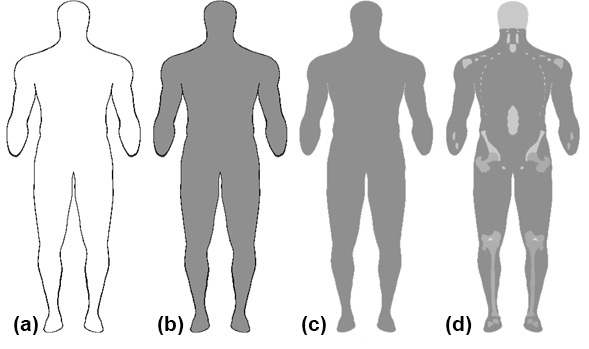
\includegraphics[width=0.95\textwidth]{IMG/Volume2.png}
    \caption{
    Cortes coronales de la imagen volumétrica en las distintas etapas del proceso de \emph{voxelización}.}
\label{fig:voxelizacion}
\end{figure}

%\todo{me gusta esta separación. Usala en el texto. Fase 1 voxelización, fase tetraedrización}
Una vez se ha construido la imagen 3D, esta se utiliza para crear una malla de tetraedros. Para la tetraedrización, se ha utilizado el algoritmo de \ac{RDT} \cite{jamin:hal-00796052}. Este algoritmo permite generar mallas de tetraedros multidominio a partir de mallas superficiales o imágenes 3D. A la hora de configurar el algoritmo, se debía alcanzar un compromiso entre precisión y eficiencia (ver apéndice \ref{anexo:criterios}). En este caso, se ha configurado con la finalidad de incrementar los tetraedros alrededor de la piel y la superficie de los huesos. De esta forma, se ha aumentado la resolución en aquellas zonas donde se requiere calcular la influencia de los huesos de forma precisa.
%permite obtener más detalle en zonas intermedias donde se resolverá la transición de pesos explicado en la siguiente sección.}
%\todo{Explica porque}

En este trabajo, se ha conseguido mantener el número de tetraedros por debajo de $3.5\times 10^6$ y el número de vértices por debajo de $8 \times 10^5$. 
%\todo{Describe la figura }
En la figura \ref{fig:tetra} se puede observar una tetraedrización del modelo \emph{ZygoteBody}$^{TM}$. Los tetraedros del interior del modelo se han coloreado de color morado, mostrando con un color diferente aquellos que pertenezcan a un hueso.
%
\begin{figure}[th]
   \centering
    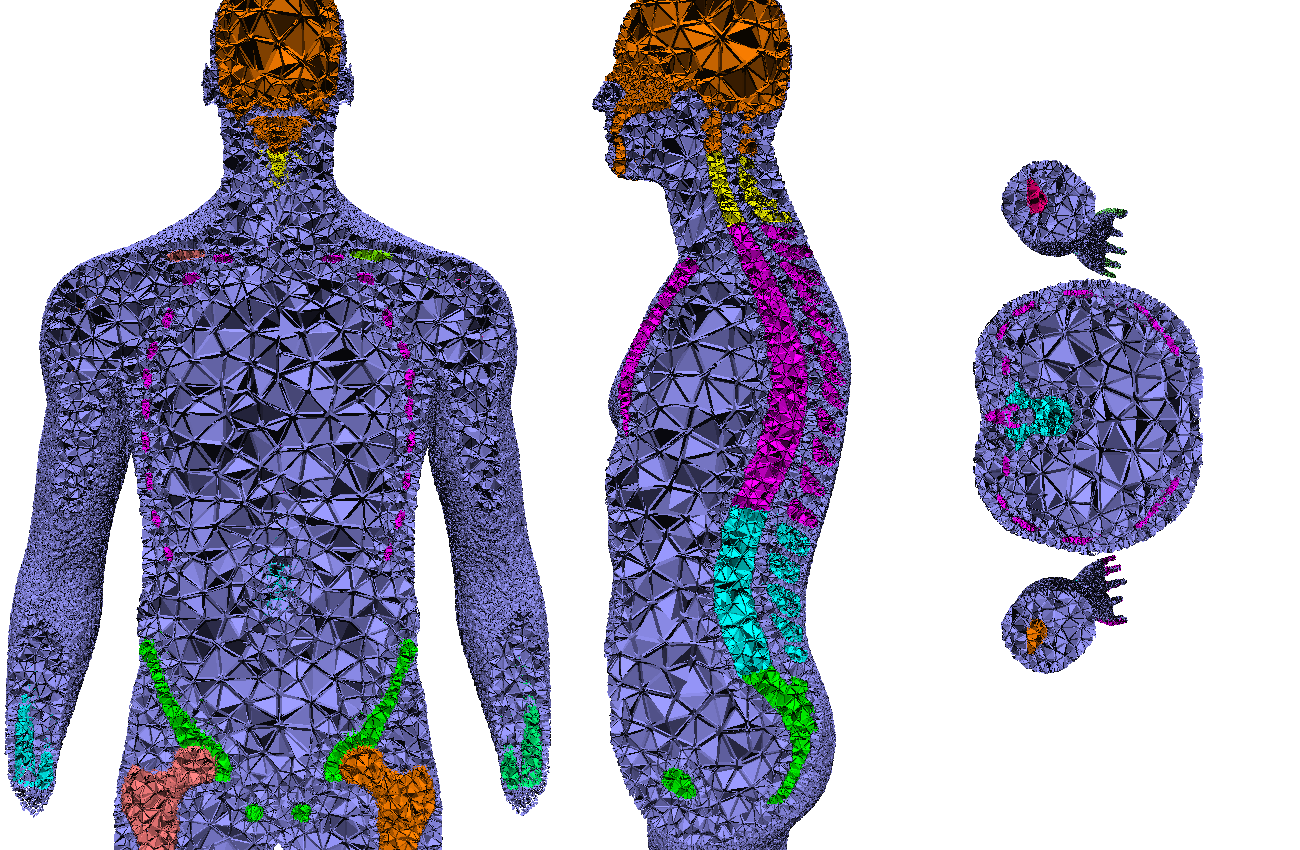
\includegraphics[width=0.95\textwidth]{IMG/boneid.png}
     \caption{Cortes coronales, sagitales y axiales mostrando el resultado de la tetraedrización. Los tetraedros morados representan el interior del modelo, mientras con diferentes colores se muestran los tetraedros etiquetados como hueso.}
\label{fig:tetra}
\end{figure} 
%\todo{Falta el color violeta}

%%%%%%%%%%%%%%%%%%%%%%%%%%%%%%%%%%%%%%%%%%%%%%%%%%%%%
\subsection{Pesado}
\label{posing:pesado}
%%%%%%%%%%%%%%%%%%%%%%%%%%%%%%%%%%%%%%%%%%%%%%%%%%%%%%
%
Como se ha introducido en el estado del arte (ver sección \ref{art:pesado}), la etapa de pesado es donde se calcula como influye el movimiento de cada hueso sobre los vértices de la malla.
Tradicionalmente, esta etapa se realiza de forma manual por un artista ayudado por una herramienta  \ac{CAD}. Aun así, existen técnicas que pueden automatizar el proceso con ciertas restricciones. \emph{Baran y Popovi\'{c}} proponen en \cite{Baran:2007} una técnica de pesado automática donde se asume que el esqueleto virtual tiene forma de modelo de alambre y la malla superficial contiene completamente dicho esqueleto.
%\new{Es habitual encontrar que las técnicas citadas estan orientadas a utilizar mallas superficiales y utilizan una recta como representación del hueso virtual para calcular su influencia en los vértices.

Esta aproximación, no es directamente aplicable al algoritmo presentado, puesto que la mayor parte de la estructuras anatómicas del paciente virtual no contienen al tejido óseo. En esta tesis, se extiende el trabajo de \emph{Baran y Popovi\'{c}} de forma que puedan utilizarse mallas volumétricas en las que el tejido óseo esté etiquetado.  
%\del{Es habitual encontrar que las técnicas citadas están orientadas al pesado en mallas superficiales. Sin embargo, como se están tratando con mallas de tetraedros, hay que adaptar estos modelos a la problemática presente. }

%
%\todo{En el paso anterior no se calculó un campo de desplazamientos. Volumetrizó el espacio interior. El pesado calcula la influencia de los huesos sobre los vértices. Esta influencia se usa para mover los vértices siguiendo el movimiento de los huesos. Una ve que se han movido los vértices se calcula el campo de desplazamientos en el interior de cada tetraedro interpolando mediante coordenadas baricéntricas el desplazamiento de los vértices. En resumen la frase es confusa cambiala}.
%\del{A su vez, tampoco se desea calcular la influencia del esqueleto virtual, sino calcular como se propagan la influencia de los tejidos óseos sobre los demás vértices de la malla de tetraedros.}
%\todo{Piensa un poco más estas dos frases}
%\todo{No entiendo bien la idea}
%\del{Así pues, en este caso se va a calcular la influencia de los huesos reales y no de los huesos virtuales a los vértices de la malla de tetraedros y no de los vértices de los distintos tejidos}
%\todo{Separa las ideas. La primera diferencia es que no se usa el esquelto virtual, sino que se propaga la influencia del tejido oseo. Diferencia 2, no se calcula la influencia sobre el resto de tejidos sino que se calcuala la influencia sobre los vertices de la malla volumetrica}. 

%\todo{Esto es muy raro. Hablas de condiciones que no están en esta este capitulo. No se si se va enteder. Por favor, cuando lo reescribas dedicale tiempo.}

%Se ha tomado como punto de partida la técnica presentada en \cite{Baran:2007}. \emph{Baran y Popovi\'{c}} describen un proceso que realiza el pesado de forma automática, 
La técnica de pesado descrita en \cite{Baran:2007} asume que la influencia de los huesos varia suavemente en la superficie de la malla. Para ello, se propone utilizar la ecuación de la difusión \ref{diffusion}, suponiendo que la influencia de un hueso se propaga como lo haría la temperatura en una superficie. 

%\todo{Transiciones de que. Desarrolla un poco más las cosas}
%\todo{Tanto calor es un poco repetitivo.}

%Existen actualmente técnicas para calcular el pesado de forma más efectiva \cite{Jacobson:2011} comentadas en el estado del arte, pero se basan en el mismo principio\todo{que no se basen en el mismo principio no es suficiente para descartarlas}. 
%Tomando en cuenta la idea original de \emph{Baran y Popovi\'{c}}\cite{Baran:2007}, se ha modificado\todo{que se ha modificado} para adaptarla al algoritmo propuesto debido a que su aplicación no es directa\todo{reescribe la frase}.



%\todo{1. Rehaz la pasiba.}. 
%En \cite{Baran:2007}, se resuelve la ecuación del calor donde se hace una analogía entre temperatura y el peso de los vértices. 
%\todo{Cual es la analogía concreta. Ademas del la difusion del calor hablas en el parrafo anterior. Tienes que hilar mejor las cosas. }
%\todo{Cuando metes una ecuación tienes que explicar los términos. }

\begin{equation}
\label{diffusion}
 \frac{\delta T}{ \delta t} = k \Delta T + q,
\end{equation}
%
donde $t$ es el tiempo, $T$ es la temperatura, $k$ es la conductividad térmica del material
y $q$ son los generadores de calor.
%\todo{revisar}

A la hora de calcular la influencia $Wj$ de cada hueso $j$, se resuelve la ecuación anterior en el caso estacionario: 
\begin{equation}
\label{diffusion1}
 0 =  \Delta W_j +  q_{k}.
\end{equation}
Ahora $q_{k}$ son las zonas de la malla superficial visibles desde el hueso $j$. Estos puntos son fuentes de influencia del hueso $k$. \emph{Baran y Popovi\'{c}} se ven obligados a introducir el término $q_{k}$ para relacionar los puntos de la superficie con el esqueleto virtual. 
%Dado que las condiciones de contorno se imponen directamente sobre la malla de tetraedros, no es necesario definir matrices de visibilidad que transfieran el calor desde los huesos virtuales a los vértices como ocurría en \cite{Baran:2007}. 
En el método propuesto en esta tesis, se dispone de una malla volumétrica del interior del paciente que se utiliza para calcular los pesos $W_j$:  
\begin{equation}
\label{diffusion2}
 0 =  \Delta W_j.
\end{equation}
La ecuación anterior se discretiza espacialmente mediante el \ac{FEM} utilizando la malla volumétrica y las coordenadas baricéntricas de los tetraedros como función de forma (para más información puede consultarse el libro \cite{Lewis2004}):  

\begin{equation}
\label{diffusion3}
 0 =  \mathbf{A} \mathbf{W_j},
\end{equation}
donde $\mathbf{W_j}$ es el vector que contiene la influencia del hueso $j$ sobre todos los vértices de la malla y $\mathbf{A}$ es la matriz de coeficientes del sistema. 
Para poder resolver la ecuación \ref{diffusion3}, se deben establecer las condiciones de contorno del problema en los vértices etiquetados como hueso. De forma que la influencia $w_{i,k}$ del hueso $k$ sobre el vértice $i$ es igual a $1$ si $k=j$ e igual a 0 si
$k \neq j$. Para introducir las condiciones de contorno se ha decidido utilizar la técnica de eliminación: 
\begin{equation}
\label{diffusion4}
 \mathbf{b_j} =  \mathbf{\hat{A}} \mathbf{W_j},
\end{equation}
donde la matriz $\mathbf{\hat{A}}$ se obtiene eliminando las filas y las columnas de los vértices que están etiquetados como hueso y  $\mathbf{b_j}$ es el vector de términos independientes que modela las condiciones de contorno del hueso $j$. Tal y como puede apreciarse en la ecuación \ref{diffusion4} la matriz $\mathbf{\hat{A}}$ es constante para todos los huesos, ya que solo depende de la discretización del dominio. Como esta matriz es simétrica y definida positiva, permite calcular la descomposición de \emph{Cholesky} una única vez y usarla para resolver el sistema lineal de cada hueso.





%\todo{No explicas los términos de la ecuación. antes de hablar de Wj yo hablaria de Wi,j. Por otro lado recuerda que los vectores debería ir en negrita. Deberías intidicar que resuelves la equación en el caso estacionario. Es uno de los motivos de que se simplifique. Cita el libro que uilizamos  }

%De esta forma, se obtiene un campo de pesos $W_j$  para cada hueso donde el tejido óseo correspondiente a $j$  propaga su influencia (temperatura 1) en el que se está resolviendo e influencia nula (temperatura 0) para el resto de huesos.  %de forma que la solución propuesta hace que la energía laplaciana sea estacionaria. Además, esta adaptación asegura una suavidad de orden superior\todo{la frase no suena bien}. 
%\todo{reescribe la frase. Da la sensación que no entiendes que escribes.: flojeo un poco en esta parte sobre todo al escribirla 1 Reformulamos el problemas haciendo cero el laplaciano. Esto es equivalente a minizar la energia. 
%Tienes que hacer un esfuerzo: 
%Ver enlace en comentarios
%https://es.wikipedia.org/wiki/Operador_laplaciano 
%}
%


%Con el objetivo de calcular  de un hueso $j$, se resuelve el caso estacionario definido en la ecuación \ref{diffusion}.%\todo{Tengo la impresion de que sueltas frases sin preocuparte de que sigan un orden logico. Esto está muy flojo.}
%\todo{Lo hablamos en persona. No me gusta la notación}

%A continuación, para calcular los pesos $W_j$, esta ecuación se resuelve para cada hueso $j$, donde se imponen las siguientes condiciones de contorno: se considera que el valor $W_j$ es $1$ (influencia) dentro de los tetraedros etiquetados como $j$; y el valor es $W_j$ es $0$ (influencia 0) dentro de los tetraedros etiquetados como $k$, donde $k$ es cualquier otro hueso que no es $j$. En el equilibrio estático, el resto de vértices tienen que verificar la ecuación \ref{ourdiffusion}. El problema se define de la siguiente manera:

% \begin{equation}
% \label{problema1}
% \Delta W(x)_{j} = 0 \\
% \end{equation}
% \begin{equation}
% \label{problema2}
% W(x)_{j} = 1\ \;
% \forall x \in B_{j} \\
% \end{equation}
% \begin{equation}
% \label{problema3}
% W(x)_{j} = 0\ \;
% \forall x \in B_{k}; k\neq j
% \end{equation}
%\new{donde $W$ es el campo de pesos definido en el dominio $x$. $j$ indica el hueso para el que se está resolviendo, mientras que B es el subdominio de $x$ que representa el hueso real.}

%
%En comparación, a un mayor número de vértices perteneciente a la malla de tetraedros, el sistema de ecuaciones resulta mucho mayor.}
%\new{Con el objetivo de resolver la ecuación \ref{problema1}, se discretiza usando \ac{FEM}  (ver \cite{Lewis2004}). La ecuación \ref{system} muestra la discretización final de la ecuación de difusión:}
%
%\begin{equation}
%\label{system}
%\mathbf{A} \mathbf{W}_j = \mathbf{b}_j,
%\end{equation}
%
%donde $\mathbf{A}$ es la matriz de coeficientes del sistema, el vector $\mathbf{b}_j$ depende de las condiciones de contorno del hueso  $j$ y $\mathbf{W}_j$ es un vector que  contiene los pesos  $w_{i,j}$ para cada vértice sin etiquetar $i$. \new{$\mathbf{A}$ es constante para todos los huesos ya que solo depende de la discretización del dominio. Como esta matriz es simétrica y definida positiva, permite calcular la descomposición de \emph{Cholesky} de esta matriz una única vez y usarla para resolver el sistema lineal de cada hueso.}

Al igual que los algoritmos de pesado clásicos, se deben cumplir las mismas condiciones, \ref{cond1} y \ref{cond2}, que se citan en la sección \ref{art:pesado}. %Es importante mencionar que esta formulación cumple con las restricciones que se imponen en \ref{cond1} y \ref{cond2}. 
Primero, se puede asegurar que el valor máximo y mínimo solo se alcanzan en los huesos (influencia $0$ o $1$).
Segundo, se puede calcular la suma de todos los vectores de pesos resolviendo el siguiente sistema:
\begin{eqnarray}
\sum^{n}_{j=1} \mathbf{\hat{A}} \mathbf{W_j} = \sum^{n}_{j=1} \mathbf{b_j} \\
\mathbf{\hat{A}} \sum^{n}_{j=1} \mathbf{W_j} = \sum^{n}_{j=1}\mathbf{b_j} \\
\mathbf{\hat{A}} \mathbf{W}=\mathbf{b},
\end{eqnarray}
donde $n$ es el número de huesos. Dado que los huesos distintos de $j$ no modifican el valor de ninguna posición del vector $\mathbf{b_j}$ se puede concluir que el vector $\mathbf{b}$ modela un escenario donde todos los huesos tienen un peso de $1$ y por tanto $\mathbf{W}$  tomará el valor $1$ en todas sus posiciones. 


%si se considera \ref{min1}  y  \ref{min2}, donde  $n$ es el número de huesos, el sistema \ref{min3} equivale a calcular los pesos donde todos los puntos del contorno tendrán un valor de $1$. Además, como el máximo y el mínimo valor es alcanzado solamente en el contorno, dará lugar a que el valor de la suma de los pesos $\mathbf{W}$ será $1$, probando la condición \ref{cond2}.
%\todo{Creo que mezclas cosas}


% \begin{equation}
% \label{min1}
% b = \sum^{n}_{j=0} b_{j} 
% \end{equation}
% \begin{equation}
% \label{min2}
% W = \sum^{n}_{j=0} W_{j} 
% \end{equation}
% \begin{equation}
% \label{min3}
% A W = b
% \end{equation}

En trabajos más actuales \cite{Jacobson:2011}, se presentaba una técnica que mejoraba la propuesta de \cite{Baran:2007}, donde se permitía crear puntos de anclaje y cajas contenedoras para controlar la animación del modelo. 
%\todo{lo que has antes de la coma no esta bien enlazado con lo que hay después.}
El inconveniente principal es la complejidad añadida al tener que resolver un problema disperso y cuadrático para imponer las restricciones. Sin embargo, la solución propuesta en esta sección solo requiere resolver un sistema de ecuaciones lineales. 
 %Por otra parte,  mientras que la técnica


%\todo{comprueba la sintaxis, parece cherokee }
 \begin{figure}[ht]
   \centering
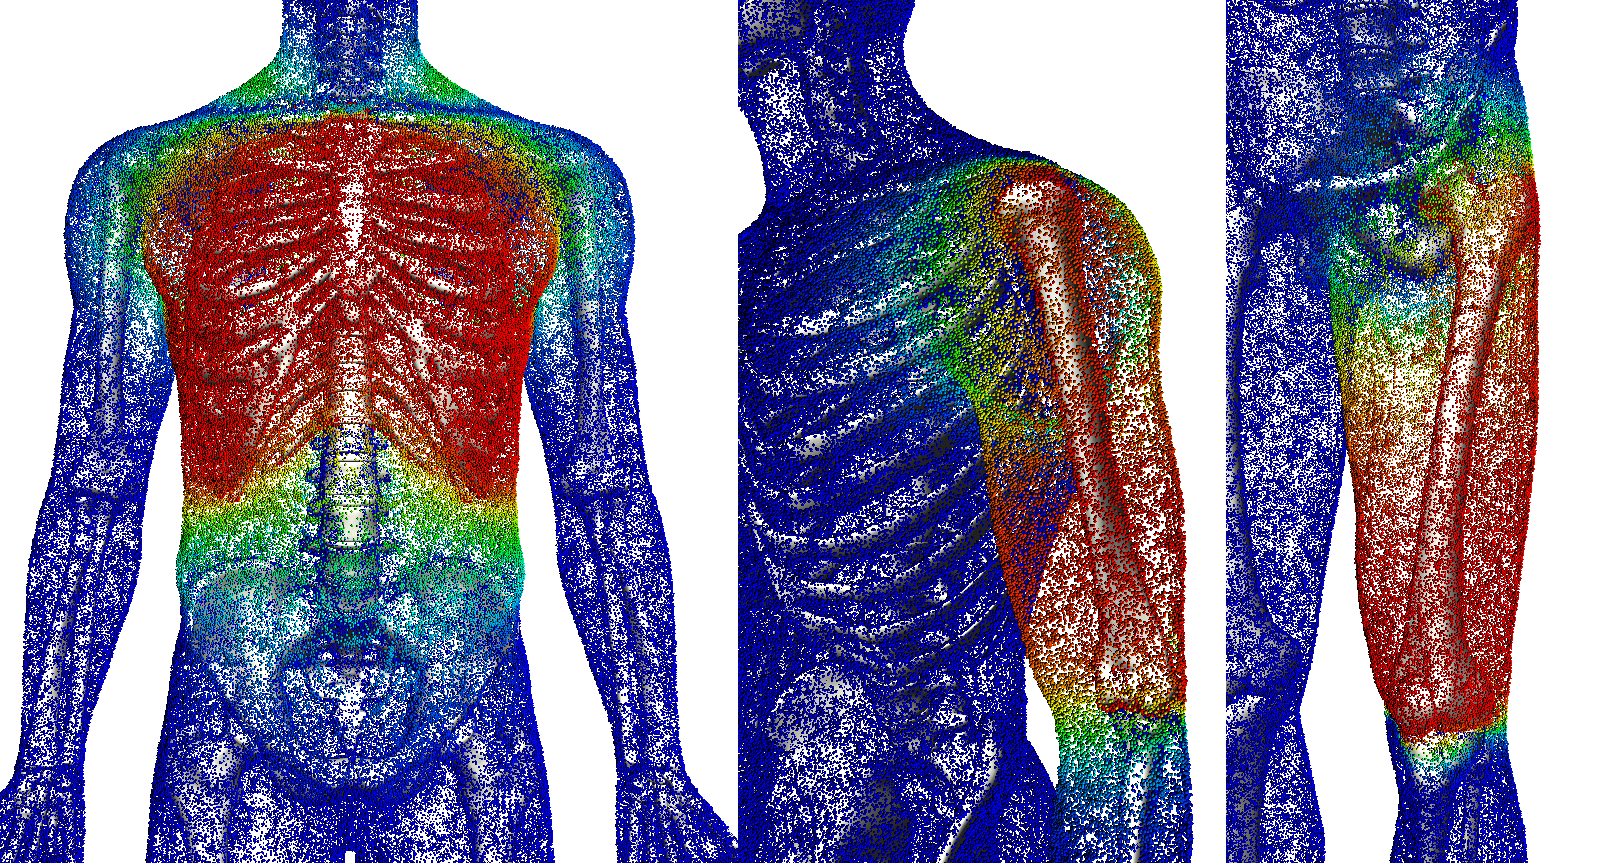
\includegraphics[width=0.9\textwidth]{IMG/weights.png}
     \caption{Influencia de algunos huesos sobre los vértices de la malla de tetraedros. En las zonas con color rojo, los pesos toman valores cercanos a 1 y en las zonas de color azul, los pesos son cercanos a 0.}
      \label{fig:pesado}
\end{figure}
 
La figura \ref{fig:pesado} muestra los resultados obtenidos con el algoritmo propuesto. Se muestra  como ejemplo la influencia de los huesos de la caja torácica, el húmero y el fémur en los vértices de la malla de tetraedros.
%\todo{La idea esta bien pero la redacción es mejorable. Reescribe las dos frases.}

%%%%%%%%%%%%%%%%%%%%%%%%%%%%%%%%%%%%%%%%%%%%%%%%%%%
\subsection{Mapeado}
\label{posing:Mapeado}
%%%%%%%%%%%%%%%%%%%%%%%%%%%%%%%%%%%%%%%%%%
%
Para poder transferir los movimientos de las articulaciones a los tejidos del paciente, hace falta relacionar cada vértice de las mallas superficiales con las que se modela la anatomía con un tetraedro de la malla volumétrica. Para ello, es necesario conocer la posición del vértice en coordenadas del tetraedro en el que recaiga. Así, se calculan sus coordenadas baricéntricas para,  de esta manera, transferir el campo de desplazamientos definido en la malla de tetraedros a los tejidos internos del paciente virtual.
%\todo{Esta frase no suena natural.}




%\new{Para calcular la influencia de los pesos de los teatraedros, se utiliza la posición del vértice que ocupa dentro de su tetraedro. Entonces, se utilizar ayuda de las coordenadas baricéntricas. }
%\todo{??????}
%
%Estas coordenadas indican la influencia de cada uno de los vértices del tetraedro al vértice que esta mapeado.
%Por tanto, hay que calcular cada una de las coordenadas baricéntricas para cada vértice de las mallas superficiales.
%\todo{De verdad que no puedo reescribir nada porque no se lo que quieres decir. Por favor rehaz todo el apartado con cuidado y ligando las ideas.}


Para encontrar el tetraedro que contiene a cada vértice de las mallas superficiales, el enfoque más simple es comprobar cada uno de los $n$ vértices con cada uno de los $m$ tetraedros, 
%
%\todo{La palabra significa suena raro en este contexto. La frase enter es rarr}
aunque este método es muy costoso ($\mathcal{O}(n \cdot m)$). Para acelerar el cálculo global, se ha utilizado la técnica \emph{Spatial Hashing} \cite{Teschner2003}. Esta técnica subdivide el espacio en regiones cúbicas, almacenando en una \ac{tabla hash} solo aquellas regiones que contengan algún tetraedro. El coste de almacenar los tetraedros en la \emph{\ac{tabla hash}} es $\mathcal{O}(m)$. Posteriormente, recorrer la lista de vértices de los distintos tejidos y asignarlos a un tetraedro tiene un coste lineal $\mathcal{O}(n)$, testeando solo los tetraedros que comparten posición en la \emph{\ac{tabla hash}}. Dado que el proceso de volumetrización elimina la piel para evitar ciertos problemas, algunos vértices se encuentran fuera de la malla volumétrica. En estos casos, se busca de forma recursiva en la \emph{\ac{tabla hash}}, el tetraedro más cercano.
De esta manera se ha reducido el tiempo que tarda el método de fuerza bruta de horas a menos de un minuto.


%\todo{No esta bien explicado}


%%%%%%%%%%%%%%%%%%%%%%%%%%%%%%%%%%%%%%%%%%%%%%%%%%%%%%
\subsection{Selección de poses}
\label{posing:Poses}
%%%%%%%%%%%%%%%%%%%%%%%%%%%%%%%%%%%%%%%%%%%%%%%%%%%%%%
%
Otro de los objetivos propuestos para este algoritmo es permitir a un médico dirija y supervise la deformación del paciente virtual de manera interactiva. %A su vez, puede guardar posturas interesantes que permitan animar los modelos automáticamente en un futuro.
En esta etapa, el usuario es el encargado de seleccionar la postura del modelo anatómico. Para ello, el algoritmo propuesto permite usar cinemática directa (fig. \ref{subfig:direct}), poses pregrabadas, animaciones (fig. \ref{subfig:animacion}) e incluso usar el dispositivo \emph{Microsoft Kinect}~\cite{shotton2013} (fig. \ref{subfig:kinect}) para capturar la pose del usuario y transferirla al paciente virtual. Aun así, técnicas como \emph{retargeting} \cite{7581666} o cinemática inversa, podrían añadirse en el futuro. %ser incluidas en el algoritmo.
\begin{figure}[ht]
    \begin{subfigure}[b]{0.32\linewidth}
        \centering
        {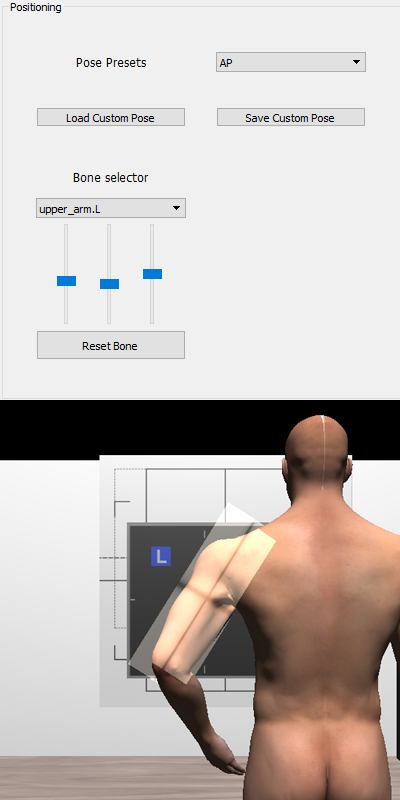
\includegraphics[width=\linewidth]{IMG/Pose1.png}}
        \caption{Posición del brazo izquierdo seleccionada por cinemática directa. \label{subfig:direct}}
    \end{subfigure}
    \null\hfill
     \begin{subfigure}[b]{0.32\linewidth}
        \centering
        {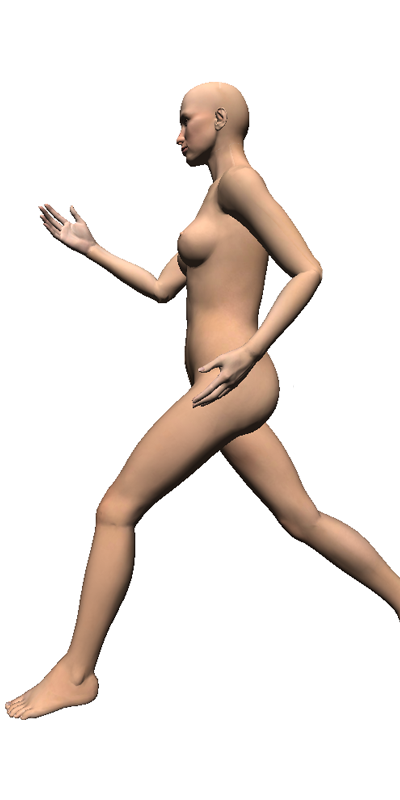
\includegraphics[width=\linewidth]{IMG/Pose3.png}}
        \caption{Extracción de la posición desde un ciclo de carrera. \label{subfig:animacion}}
    \end{subfigure}
    \null\hfill
     \begin{subfigure}[b]{0.32\linewidth}
        \centering
        {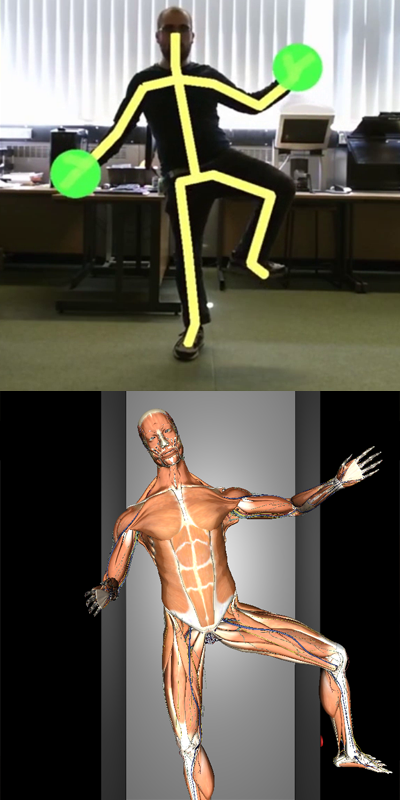
\includegraphics[width=\linewidth]{IMG/Pose2.png}}
        \caption{Selección de pose utilizando la tecnología de \emph{Microsoft Kinect}. \label{subfig:kinect}}
    \end{subfigure}
    \caption{\label{fig:selecpose} Ejemplo del posicionamiento de un paciente virtual.}
   \end{figure}

En la animación esqueletal, para transferir el movimiento del esqueleto virtual a la malla superficial, se pueden utilizar diferentes algoritmos de \emph{skinning} (ver sec. \ref{art:skinning}). %\todo{el skinning no es un modelo matematico, son los algoritmos que transfieren el movimiento de los usos... Tal y como esta redacto parece que en el estado del arte has anticipado que TU ALGORITMO USARA EL SKINNING}.
%En el caso del algoritmo propuesto, se puede tratar los vértices de los tetraedros como vértices de una malla superficial\new{????}. De la misma manera que la animación clásica las animaciones esqueletales son transferidas a la malla volumétrica usando una técnica de \emph{skinning}. Los tetraedros deformados definen un campo de deformación que se utiliza para animar todos los tejidos del paciente virtual.
En el caso del algoritmo propuesto, las técnicas de  \emph{skinning} se aplicarán a los vértices de la malla de tetraedros en lugar de aplicarse directamente a las mallas superficiales. Los vértices del resto de tejidos del modelo serán transformados gracias al campo de desplazamientos definido en la malla volumétrica. Dicho campo se obtendrá de forma implícita interpolando el desplazamiento de los vértices de cada tetraedro en su interior, utilizando coordenadas baricéntricas para trasladar la deformación al paciente virtual. 

%\todo{A partir de ahora solo voy a dar pinceladas. Llevo la mañana del viernes, la del sabado y la del domingo y no avanzo. No puedo comentar cada frase. Es TU RESPONSABILIDAD cuidar la redacción. }


Se ha elegido implementar la técnica de \emph{skinning} descrita en \cite{le2016real},  ya que el método \ac{COR} resuelve algunos de los problemas de \ac{DQS} y \ac{LBS} descritos en la sección \ref{art:skinning}. El algoritmo se basa en calcular, en preproceso, los centros de rotación óptimos para todos los vértices de la malla. %En este caso, es necesario  de tetraedros\todo{paredce que son ellos trabajan con mallas de tetrahedros}. 
Una vez se calcula esta información, el rendimiento del algoritmo es muy similar al de otras técnicas como \ac{LBS} y \ac{DQS}. %Estas tres técnicas son intercambiables entre si debido a que están perfectamente diseñadas para usarse con las arquitecturas gráficas modernas.
Este algoritmo se basa en que los vértices con un pesado similar deben seguir las mismas transformaciones que sus vecinos. En su trabajo, \emph {Le y Hodgins} ~\cite{le2016real} proponen una función de similaridad  $s(\textbf{w}_p,\textbf{w}_s)$ con la que ponderar la contribución de los vecinos según lo parecidos que sean sus pesos:
%\todo{pasivas, intercambiables????}

%\begin{eqnarray}\nonumber
\begin{equation}
\label{similarity}
 s(\textbf{w}_p,\textbf{w}_s) = 
\sum_{\forall i \neq j} w_{p,i}w_{p,j}w_{s,i}w_{s,j}\exp-\frac{(w_{p,i}w_{s,j}-w_{s,i}w_{p,j})^2}{\sigma^2}
\end{equation}
%\end{eqnarray}
\normalsize
%
donde $\textbf{w}_p$ y $\textbf{w}_s$ son vectores de los pesos de los vértices $p$ y $s$, y se realiza la suma para todas las combinaciones de pares de huesos $i$ y $j$ . Por último, $\sigma$ parametriza la función exponencial. 
%\todo{faltan parámetros}
En el estudio que aquí se presenta se ha utilizado un valor de  $\sigma=0.1$. 

La función de similaridad se utiliza posteriormente para calcular el centro de rotación $\textbf{cor}_p$ de cada vértice $p$. En la presente tesis, se ha adaptado la ecuación  propuesta en \cite{le2016real} de forma que pueda utilizarse en mallas volumétricas. Así, la ecuación se quedará de la siguiente manera: 
%
\begin{equation}
%\begin{eqnarray}\nonumber
\textbf{cor}_p = 
\frac
  {
  \sum_{\forall t \in T}
    s(\textbf{w}_p,
      \frac{\textbf{w}_{t1}+\textbf{w}_{t2}+\textbf{w}_{t3}+\textbf{w}_{t4}}{4})
    %\frac{\textbf{v}_{t1}+\textbf{v}_{t2}+\textbf{v}_{t3}+\textbf{v}_{t4}}{4}
    V_t\mathbf{c}_t
  }
  {
  \sum_{\forall t \in T}
    s(\textbf{w}_p,
      \frac{\textbf{w}_{t1}+\textbf{w}_{t2}+\textbf{w}_{t3}+\textbf{w}_{t4}}{4})
    V_t
  } ,
%\end{eqnarray}
\normalsize
\end{equation}
%
donde $\textbf{cor}_p$ es el nuevo centro de rotación del vértice $p$, $t$ es el tetraedro de la malla de tetraedros $T$, $V_t$ es el volumen del tetraedro $t$, $\textbf{c}_t$ es el centroide del tetraedro $t$ y $\textbf{w}_{t1}$, $\textbf{w}_{t2}$, $\textbf{w}_{t3}$ y $\textbf{w}_{t4}$ son los pesos de los vértices del tetraedro $t$. Una vez calculado este centro, se puede usar en la etapa interactiva utilizando el \emph{shader} descrito en \cite{le2016real}.

Finalmente, para animar los vértices de cada malla, el campo de desplazamiento de un punto dentro de un tetraedro se puede calcular interpolando el desplazamiento de cada uno de sus vértices. Se interpola este campo usando las coordenadas baricéntricas de cada tetraedro, ya calculadas en el paso de pesado (sec. \ref{posing:pesado}). Matemáticamente, el campo de desplazamientos calculado es continuo pero no diferenciable dentro de la malla volumétrica y permite calcular una matriz de transformación constante por cada tetraedro (consultar \cite{Muller2004}). Esta matriz de transformación, perteneciente al tetraedro, se aplica a cada uno de los vértices de la malla superficial asociados al tetraedro. Estos cálculos se realizan en la tarjeta gráfica para mejorar el rendimiento del algoritmo.

%\todo{No se si este apartado se entiende lo basta bien. Es muy criptioco. Redactado, a ver que tal}


% %%%%%%%%%%%%%%%%%%%%%%%%%%%%%%%%%%%%%%%%%%%%%%%%%%%%%%
 \subsection{Optimización}
\label{posing:optimizacion}
% %%%%%%%%%%%%%%%%%%%%%%%%%%%%%%%%%%%%%%%%%%%%%%%%%%%%%%
% %

% %

%Los resultados de la etapa previa son visualmente realistas\todo{¿Como lo sabes?}. \ac{COR} reduce el volumen ganado por \ac{DQS} o el volumen perdido por \ac{LBS}\todo{tienes resultados que lo respalden}. Aun así, hay algunos escenarios dónde se produce un cambio apreciable de volumen.El algoritmo propuesto permite al usuario refinar la solución usando un algoritmo basado en físicas
La mayoría de los cauces de animación se basan en transferir el movimiento de un esqueleto virtual a una \acl{B-rep} del personaje mediante un algoritmo de \emph{skinning}. Estos, suelen presentar el problema de garantizar la conservación del volumen. Las pérdidas y ganancias de volumen son comportamientos no deseados, especialmente, teniendo en cuenta que el cuerpo humano está compuesto principalmente por agua, un líquido incompresible. Por este motivo, se ha implementado un paso opcional que optimiza el resultado obtenido en la fase de \emph{skinning}. Esta técnica está basada en la formulación co-rotacional del \ac{FEM}. Cabe destacar que el objetivo de este paso es mejorar la conservación de volumen y no el de simular biomecánicamente el comportamiento de los distintos tejidos. Por este motivo, no se requiere de la caracterización mecánica del paciente virtual.  

%Aunque se haya decidido utilizar un enfoque geométrico para el algoritmo, adicionalmente, se ha propuesto utilizar un modelo basado en físicas que permita al usuario refinar el resultado obtenido. Sin las descripciones mecánicas de los tejidos, se ha propuesto una solución que busca la conservación del volumen de cada tetraedro. Al no disponer de todos los tejidos o de las propiedades mecánicas, el objetivo de esta etapa no es conseguir un solución realista sino, mejorar el aspecto visual del resultado. }

%se puede decir que todos los tejidos están compuestos de agua y se asume que es un fluido incompresible y por tanto, las deformaciones tienen que permitir la conservación de volumen para cada tetraedro.}


%\todo{ponemos fórmulas que tenías en los comentarios?}
%\todo{Si eres capaz de explicarlo...}

El modelo físico utilizado está basado en un modelo mecánico estacionario:
\begin{eqnarray}
\nabla \cdot \mathbf{\sigma} = 0,
\end{eqnarray}
donde $\mathbf{\sigma}$ es el tensor tensión. También, se emplea un modelo elástico isotrópico, homogéneo y lineal:  
\begin{eqnarray}
\mathbf{\sigma} = \mathbf{E}\mathbf{\epsilon}, 
\end{eqnarray}
donde $\mathbf{E}$ es la matriz que define el comportamiento elástico del material y $\mathbf{\epsilon}$ es el tensor de \emph{Cauchy}. Es importante destacar que el tensor de \emph{Cauchy} no está indicado para medir grandes deformaciones.  Debido a su naturaleza lineal, las rotaciones generan distorsiones en la geometría al interpretarlas como deformaciones, produciendo efectos de escalado o abultamientos. Para solucionar esta problemática, se utiliza la formulación co-rotacional del \ac{FEM} para resolver el sistema. La volumetrización del modelo (sec. \ref{posing:volumetrizacion}) se utiliza como discretización espacial y las posiciones de los huesos como las condiciones de contorno necesarias para resolver el problema estático. Para más información se puede consular \cite{Muller2004}.

Con la intención de controlar el modelo elástico planteado, se utilizan los parámetros \emph{ratio de Poisson} y \emph {módulo de Young}. El \emph{ratio de Poisson} controla la conservación del volumen, donde un valor de $0.5$ garantiza su conservación. Sin embargo,  se utiliza un valor ligeramente inferior para asegurar la estabilidad numérica. 
Por otro lado, el comportamiento elástico del material se caracteriza con el valor del \emph {módulo de Young}. Se va a utilizar un material homogéneo, ya que el valor de este parámetro es irrelevante desde el punto de vista teórico y, por tanto, se elegirá su valor con el objetivo de mejorar la estabilidad numérica del sistema. 
Para ello, se ha analizado la matriz de coeficientes del sistema para varios valores del módulo y se ha seleccionado aquel valor que haya maximizado su condicionante.

La formulación co-rotacional calcula las fuerzas internas (aquellas derivadas de la deformación) tras deshacer las rotaciones de cada elemento de la malla. Después, se rotan las fuerzas para ajustarlas a la configuración final del elemento~\cite{Muller2004}. Dado que esta técnica necesita conocer las rotaciones finales que se aplican a cada elemento de la malla, el problema estático se ha de resolver de forma iterativa. Para acelerar la convergencia del algoritmo, se utiliza la deformación seleccionada por el usuario como situación inicial reduciendo  significativamente el número de iteraciones requeridas para llegar a la solución final.  %(ver Fig. \ref{x}). 

Para conocer los desplazamientos de los vértices de la malla de tetraedros se ha formulado un sistema de ecuaciones lineales. Según las propiedades anteriormente citadas, la matriz de coeficientes del sistema lineal es dispersa, simétrica y definida positiva. Este tipo de sistemas de ecuaciones se pueden resolver utilizando el método del gradiente conjugado \cite{Press2007}. La convergencia de estos métodos se acelera con el uso de pre-condicionadores (ver \cite{hauth2003}). En el caso planteado, se utiliza un precondicionador de \emph{Jacobi} y, además, como solución inicial se utiliza la posición del modelo calculada en la etapa de \emph{skinning}. %Para acelerar esta etapa, se utiliza  como solución inicial la posición del modelo ya calculado en la etapa de selección de poses (sec. \ref{posingPoses}), además de emplear un precondicionador de Jacobi.

Finalmente, se utilizarán los desplazamientos de los vértices de los tetraedros para calcular la transformación que se aplicará a todos los tejidos asociados a cada elemento de la malla volumétrica, como se ha detallado en la sección \ref{posing:Poses}.% (ver sec. \ref{posing:Poses}). 

\subsection{Animación de representaciones volumétricas}
\label{posing:animvol}


%\todo{explica el por qué: el campo de desplazamientos, me he traido esto para inspirarme}

Como se puede leer en la sección 
\ref{posing:method}, el algoritmo se basa en el cálculo de un campo de desplazamientos continuo (ver sec. \ref{posing:volumetrizacion}) %\todo{si no es continuo todo lo que dices a continuación no sirve}
en el interior del paciente virtual que permita transformar sus estructuras internas. Esto permite deformar los tejidos de forma independiente y, aun así, garantizar que estos se muevan solidariamente. Se ha decidido deformar los tetraedros y posteriormente interpolar el movimiento a los vértices usando las coordenadas baricéntricas, en lugar de transferir los pesos calculados (ver sec. \ref{posing:pesado}) de los tetraedros a los vértices interiores. 
De esta forma, el campo de desplazamientos definido se puede usar para transformar tanto vértices de representaciones superficiales como \emph{vóxeles} en modelos volumétricos. 


En la figura \ref{fig:volEx} se muestran los pasos para obtener una deformación de una representación volumétrica. En primer lugar, se genera la malla de tetraedros del modelo utilizando la misma técnica explicada en la sección \ref{posing:volumetrizacion}  y se calculan los pesos como se detalló en la sección \ref{posing:pesado}. A partir de esta \emph{tetraedrización}, se definen una serie de \emph{píxeles} dentro de cada tetraedro en la posición deformada. Se mapean con la configuración de reposo utilizando la transformación inversa del campo de desplazamiento. Para ello, se itera sobre cada caja contenedora de la \emph{\ac{tabla hash}} y se utilizan las coordenadas baricéntricas. Este proceso, al ser fácilmente paralelizable en \ac{GPU}, permite que se pueda \emph{renderizar} en tiempo real.


\begin{figure*}[!ht]%[b]%[b!ht]
   \centering
   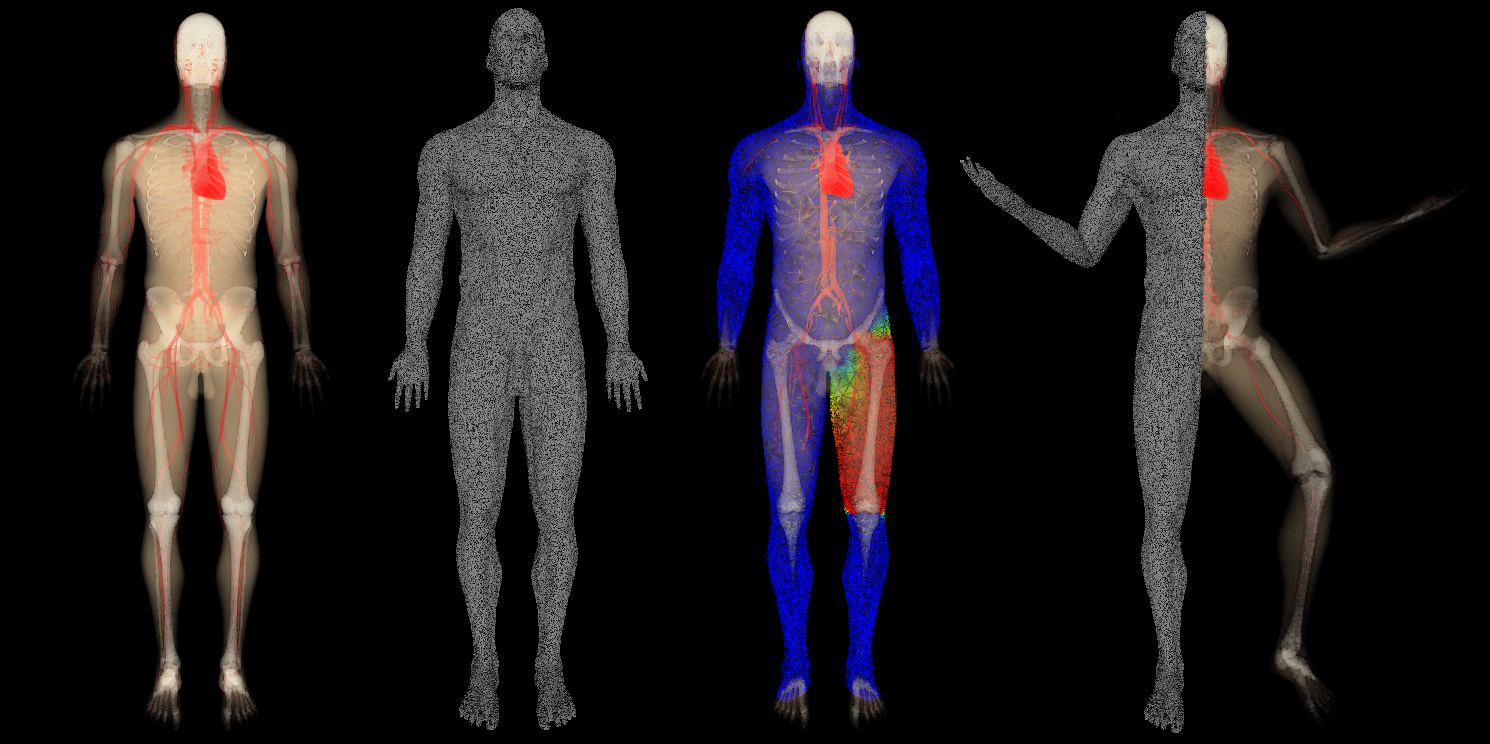
\includegraphics[width=0.90\textwidth]{IMG/Volumetric}
    \caption{Proceso de animación para modelo volumétrico. De izquierda a derecha: (1) modelo volumétrico en reposo, (2) malla de tetraedros generada, (3) malla de tetraedros representando el peso del fémur como ejemplo (rojo significa influencia cerca de 1, azul influencia 0) y (4) malla de tetraedros superpuesta al modelo volumétrico deformado. }
    \label{fig:volEx}
\end{figure*}


%%%%%%%%%%%%%%%%%%%%%%%%%%%%%%%%%%%%%%%%%%%%%%%%%%%%%%%%%
\section{Detalles de implementación}
\label{posing:preprocess}
%%%%%%%%%%%%%%%%%%%%%%%%%%%%%%%%%%%%%%%%%%%%%%%%%%%%%%%%%

Como se puede leer en la sección \ref{posing:req}, la selección de poses debe ser supervisada por un usuario y, por tanto, se debe permitir la animación del modelo de forma interactiva. 
Las etapas de \emph{rigging}, \emph{volumetrización}, \emph{pesado}, \emph{mapeado} y el \emph{cálculo de los centros de rotación} son las etapas más costosas computacionalmente. 
Por este motivo, dado que solo se tienen que ejecutar una única vez por paciente virtual, se puede realizar un preproceso, almacenando los datos auxiliares generados adjuntos al modelo anatómico. 

Para facilitar la interacción, se ha creado una interfaz donde el usuario podrá manipular las articulaciones del paciente virtual, interactivamente y conseguir la transformación del modelo mientras es mostrado por pantalla 

Por último, la etapa de \emph{optimización} no es posible que se ejecute interactivamente. Esto depende del tamaño de la malla volumétrica resultante. Por ello, se deja a elección del usuario cuando se procede a ejecutar esta etapa.




%%%%% RASIMAS
\chapter{RASimAs} 
\label{cap:rasim}

%Ideas: Este capitulo se presenta un caso del uso del algoritmo detallado en el capitulo anterior. En este caso la posición del paciente se adapta en preproceso. Es decir antes de que comience la simulación. Aunque el procedimiento es supervisado, por lo que la selección de poses debe funcionar en tiempo-real una vez seleccionada la posé se pude aplicar la fase de optimización del algoritmo. Por el contrario en la herramienta de rayo X, la modificación de la pose es en tiempo real por lo que no se puede usar la etapa de optimización. PONLO BONITO}

En este capítulo se presenta un caso de uso donde se ha integrado el algoritmo propuesto en el capítulo \ref{cap:posing}. El objetivo es adaptar la posición del paciente virtual en la \emph{suite} \ac{ITGVPH} (ver sec. \ref{art:rasimas}) que prepara los modelos con los que se trabajará en el simulador \ac{RASim}. Este proceso debe ser automático exceptuando la selección de poses. El profesional médico deberá supervisar la deformación producida, debido a que no se dispone de descripciones completas o mecánicas del modelo anatómico. También, se permitirá al usuario poder ejecutar la fase de optimización ya que, en este caso, la interactividad no es crítica. %En el siguiente capítulo, el segundo caso de uso primará la interactividad, por la cual esta etapa será omitida.


%El algoritmo propuesto en el capítulo anterior ha sido incorporado en la herramienta \ac{ITGVPH} (ver sección \ref{intro:context}) que se encargará de generar la base de datos necesaria para que los usuarios puedan entrenar con una variabilidad anatómica extensa. Esta herramienta será la encargada de crear los pacientes virtuales que se utilizarán en el simulador \ac{RASim}. Esto permite al usuario enfrentarse a diferentes tipos de situaciones y mejorar el entrenamiento del procedimiento. En este capítulo se mostrarán las contribuciones aportadas en la integración de esta herramienta dentro del proyecto \ac{RASimAs}.

%Uno de los objetivos del proyecto \ac{RASimAs} es crear un simulador médico (\ac{RASim}) para entrenar en el procedimiento \ac{RA}. 


%\del{Adicionalmente, también se describirá todas las contribuciones que se han realizado con el objetivo de construir el prototipo del simulador \ac{RASim}. Este simulador permitirá validar si la salida de la herramienta \ac{ITGVPH} es útil para el entrenamiento.}

Así mismo, en este capítulo también se detallarán las contribuciones realizadas al simulador \ac{RASim} con el desarrollo del módulo \ac{Courseware} como herramienta de entrenamiento y autoevaluación.

%\del{Se ha desarrollado una aplicación de entrenamiento y autoevaluación para que el simulador se use como herramienta de aprendizaje del procedimiento de \ac{RA}. 
%El simulador médico \ac{RASim} da la posibilidad de entrenar el procedimiento utilizando material médico similares como las agujas y la sonda de ultrasonidos con la intención de permitir a los usuarios entrenar el procedimiento y desarrollar sus habilidades tanto cognitivas y no cognitivas, ayudando a mejorar su confianza en el procedimiento. El usuario podrá elegir entre modos de entrenamiento, donde la  aplicación registrará métricas de rendimiento con el objetivo de proporcionar retroalimentación sumativa y formativa.} %Además, este simulador dispone de una base de datos que permita al médico en formación experimentar multitud de variabilidades anatómicas generadas a partir de otros modelos o de imágenes médicas. 










%%%%%%%%%%%%%%%%%%
\section{Herramienta TPTVPH}
\label{rasim:posing}

La \emph{suite} \ac{ITGVPH} se encargará de generar la base de datos necesaria para que los usuarios puedan entrenar con una variabilidad anatómica extensa. Esto permite al usuario enfrentarse a diferentes tipos de situaciones y mejorar el entrenamiento del procedimiento. En ocasiones el procedimiento médico que se va a realizar necesita que los modelos virtuales disponibles se encuentren en una posición diferente a la postura que presentan. Por lo tanto, surge la necesidad de incluir un algoritmo que adapte un paciente virtual.

%
%Para modificar esa postura, se necesitaría un algoritmo que sea capaz de transformar un modelo virtual con estructuras internas de una pose a otra. Debido que en la mayoría de las ocasiones, no se dispone de todos los tejidos o de sus propiedades mecánicas, este método deberá ser capaz de generar deformaciones plausibles útiles para el entrenamiento.


%La tarea 3.5 del \del{ac{WP} 3} define el requisito de que la herramienta \ac{ITGVPH} permita adaptar la posición del paciente virtual creado de una postura inicial a la requerida por el simulador \ac{RASim}. 
Para ello,  se va a incorporar el algoritmo propuesto, descrito en el capítulo \ref{cap:posing}, a una aplicación llamada \ac{TPTVPH}. Esta herramienta se ha construido para proporcionar una interfaz donde el usuario pueda seleccionar la postura del paciente virtual. De esta forma, un usuario con perfil sanitario podrá seleccionar y validar las posiciones que sean requeridas en el procedimiento médico que se desee simular.



%Para ello, se ha habilitado una ventana utilizando la librería \emph{OpenGL}\ref{adsf} y \emph{Qt}\ref{asdf}\todo{revisar} permitiendo al usuario pueda manipular el modelo anatómico desde todas las posiciones que necesite.
Como primer paso, se ha dotado a la interfaz de una ventana donde el usuario puede observar el modelo anatómico. Con el objetivo de poder confirmar las correctas deformaciones del paciente virtual, el usuario puede interaccionar con la escena, de esta forma, y de manera intuitiva puede utilizar el ratón para mover, rotar, acercar o alejar el modelo y poder supervisar la deformación desde todos los ángulos posibles.

En segundo lugar, para permitir la selección de poses, se han incluido en la interfaz botones y actuadores, que permiten al usuario seleccionar las articulaciones del \ac{VPH} una a una y definir sus movimientos respecto a los centros de rotaciones calculados (ver sec. \ref{posing:rigging}). El usuario puede revisar poses anteriormente almacenadas, modificarlas y guardarlas de nuevo. También, con el objetivo de introducir movimientos más orgánicos, el sistema permite cargar animaciones provenientes de \ac{MoCap}, o utilizar la tecnología del dispositivo \emph{Microsoft Kinect} en forma de espejo para definir la postura del \ac{VPH} (ver sec. \ref{posing:Poses}).

Además, se ha incorporado una funcionalidad que permite al usuario decidir si quiere esconder tejidos con la finalidad de contemplar la anatomía interna que estuviera oculta. De esta manera, se permite dejar de \emph{renderizar} la piel o los músculos para contemplar otros órganos.% más profundos. 

Finalmente, se ha delegado la responsabilidad de generar posiciones correctas o realistas al usuario. En la sección \ref{posing:optimizacion}, se presenta una etapa optimización que se apoya en un modelo basado en física para mejorar el resultado obtenido. Al ser una etapa no interactiva, solo se activa cuando el usuario decide utilizarla. Una vez terminado el proceso, se podrá observar los resultados y almacenar el paciente virtual obtenido que será utilizado en las demás etapas de la \emph{suite} \ac{ITGVPH}.  

%Por último,  ha sido necesaria la adaptación del sistema para poder adecuarse a los formatos de fichero de entrada y salida de los modelos anatómicos. El formato elegido es \ac{X3D} de manera que será utilizados tanto por la herramienta \ac{ITGVPH} como por el simulador \ac{RASim}.

%\subsection{Interfaz de usuario \ac{TPTVPH}}
\paragraph{Interfaz de usuario \ac{TPTVPH}}\mbox{}\\



%Como se ha comentado anteriormente, el usuario puede realizar la fase de posicionamiento de manera semiautomática, dónde es éste el que supervisa y realiza por sí mismo la deformación del modelo anatómico gracias a la interfaz de usuario de la herramienta \ac{TPTVPH} que proporciona una visualización 3D del modelo.
En la figura \ref{fig:posui} se muestra la interfaz donde el usuario puede manejar las articulaciones que disponga el paciente virtual para conseguir la posición deseada. Se divide en las siguientes partes: 
\begin{enumerate}
    \item En la primera división se permite al usuario seleccionar y manipular las articulaciones por separado. %que servirá para que la herramienta \emph{ITGVPH} actúe de manera automática.
    Además, se podrán cargar configuraciones realizadas previamente o guardar posiciones del modelo en un archivo auxiliar. El propio usuario es el encargado de que la combinación de uno o más movimientos de articulaciones sean válidas para el entrenamiento del procedimiento médico. 
    \item Esta división sirve para ocultar o mostrar las distintas estructuras anatómicas que se hayan cargado en la aplicación. Esto es especialmente útil si el usuario requiere comprobar cómo se deforma la anatomía interna sin que otros tejidos la oculten. %superiores la oculten.
    \item En la interfaz 3D se puede observar el paciente virtual cargado y, gracias al ratón, el usuario puede navegar en la escena para poder observar el modelo desde cualquier perspectiva. Además, en la barra superior se muestran unos botones que realizan funciones adicionales:
    \begin{enumerate}
   \item Guardar una instantánea de la escena que el usuario está viendo. 
   \item Activar la fase de optimización a demanda del usuario. 
   \item Activar la animación precargada que puede ser utilizada para seleccionar una pose. 
   \item Permitir devolver la cámara de la escena a su posición original. 
   \item Permitir utilizar la tecnología \emph{Microsoft Kinect} para posicionar el modelo anatómico.
   \item   Permitir al usuario terminar con el posicionamiento y cerrar la aplicación.
    \end{enumerate}
    
\end{enumerate}
\begin{figure}[htbp]
    \centering
    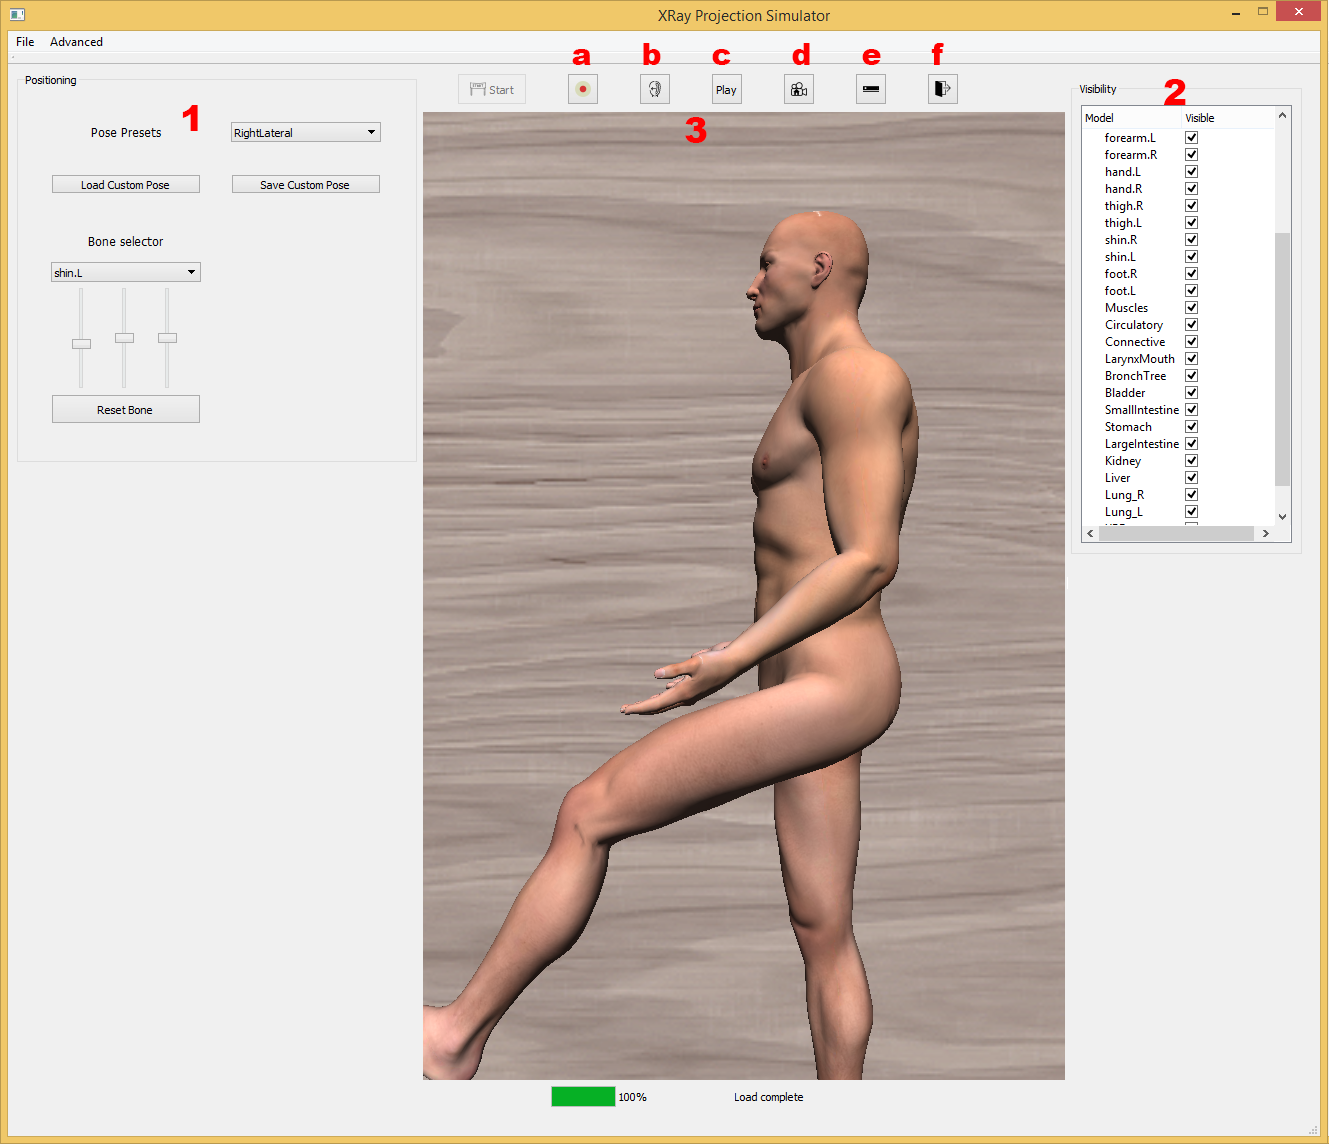
\includegraphics[width=0.9\textwidth]{IMG/posingui.png}
    \caption{Interfaz de usuario de \acs{TPTVPH} para la realización de poses. 1: Interfaz para modificar la postura del paciente virtual. 2: Lista de todos los modelos anatómicos que contenga el paciente virtual. 3: Ventana que muestra la escena virtual y en la barra superior se encuentran botones auxiliares.}
    \label{fig:posui}
\end{figure}



\section{Integración en  ITGVPH}
\label{rasim:herramienta}

%La herramienta \ac{ITGVPH} nace con el objetivo de conseguir una base de datos extensa de pacientes virtuales medios que representen una gran variabilidad anatómica. Además, permite transformar estos modelos de pacientes virtuales usando un conjunto de poses guardadas con anterioridad. %Estas poses tienen que ser generadas por un profesional cualificado a través de una interfaz de usuario, que permita al supervisor realizar cuantas posiciones se necesiten para distintos modelos anatómicos diferentes. 

Dentro del proyecto \ac{RASimAs}, el \acs{WP} 3 define todas las tareas que son necesarias para la creación de la \emph{suite} \ac{ITGVPH}, donde la tarea 3.6 se encarga de la integración
del resto de tareas. El equipo de \ac{FORTH} ha liderado el proceso de integración de todas las tareas que contó con la colaboración activa del autor de esta tesis.



% El principal objetivo es la interconexión de las etapas para conseguir la automatización de la herramienta. Por ello, los diferentes resultados producidos por cada tarea tienen que ser recogidos por esta herramienta para generar pacientes virtuales que serán utilizables tanto por el simulador \ac{RASim}. La herramienta será la encargada de las diferentes etapas para construir \ac{VPH}, desde la adquisición y procesamiento de las imágenes médicas (\ac{TC}, \ac{IRM}, etc...), el enriquecimiento el \ac{VPH} con ayuda de modelos \emph{ZygoteBody}$^{TM}$\cite{kelc2012zygote}, la adaptación del modelo de una postura a otra y la generación de las representaciones visuales y mecánicas necesarias que se utilizan finalmente en \ac{RASim}. Todas estas tareas han sido diseñadas para que puedan ser enlazadas unas con otras compartiendo el formato en su entrada y salida para automatizar la herramienta y eliminar la necesidad de tener conocimientos técnicos para poder completar todo el cauce. 
% La salida de \ac{ITGVPH} consiste en una representación superficial y volumétrica que será utilizada en el entorno de entrenamiento.




% \subsection{Caso de uso}
% \label{rasim:casodeuso}
% A continuación, se va a describir el caso de uso de la herramienta \ac{ITGVPH} que permite crear un \ac{VPH}.

% En este escenario, un usuario (profesional sanitario) puede iniciar el proceso seleccionando las imágenes médicas almacenadas en una base de datos. Estos datos suelen estar agrupados por región anatómica y existen variedad entre ellos. A continuación, el usuario podrá seleccionar los parámetros biomecánicos que se incorporarán en el modelo final, y a partir de aquí, la herramienta \ac{ITGVPH} toma el control y lanza las etapas de la herramienta con los datos de entrada seleccionados. Si se requiere, la herramienta \ac{TPTVPH} mostrará una interfaz de usuario por si es necesario modificar la postura del \ac{VPH}, pero puede elegirse una configuración anteriormente definida. En la sección anterior se ha descrito el desarrollo de la herramienta \ac{TPTVPH} que permite la adaptación del modelo anatómico.
% La salida de la herramienta consiste en dos archivos que contienen la representación superficial y volumétrica (en formato \ac{X3D} y \ac{VTU} respectivamente) del modelo generado. Estos ficheros están preparados para utilizarse en el entorno de entrenamiento utilizando \ac{RASim}.

%el usuario inicia el proceso seleccionando un conjunto de imágenes médicas que provienen de una base de datos. Estos datos suelen estar agrupados por región anatómica y existen variedad entre ellos. A continuación, el usuario puede definir o cargar un fichero dónde se encuentren los parámetros biomecánicos que se vayan a utilizar en los tejidos de la región seleccionada. El usuario puede seleccionar también si quiere alguna pose predefinida o quiere realizarla por sí mismo en una ventana interactiva. A partir de entonces, la herramienta toma el control y lanza las etapas de la herramienta con los datos de entrada seleccionados. La salida de la herramienta consiste en dos archivos que contienen la representación superficial y volumétrica (en formato \ac{X3D} y \ac{VTU} respectivamente) del modelo generado. Estos ficheros están preparados para utilizarse en el entorno de entrenamiento utilizando \ac{RASim}.

%De esta manera, un usuario (un profesional sanitario) puede iniciar el proceso seleccionando las imágenes médicas almacenadas en una base de datos. A continuación, el usuario podrá seleccionar los parámetros biomecánicos que se incorporarán en el modelo final, y a partir de aquí, la herramienta \ac{ITGVPH} toma el control, donde suministra y recoge los datos necesarios de cada etapa. Si se requiere, la herramienta \ac{TPTVPH} mostrará una interfaz de usuario por si es necesario modificar la postura del \ac{VPH}, pero puede elegirse una configuración anteriormente definida. En la sección anterior se ha descrito el desarrollo de la herramienta \ac{TPTVPH} que permite la adaptación del modelo anatómico.

%\subsection{Arquitectura lógica}
%\label{rasim:arq}

En las etapas iniciales del proyecto \ac{RASimAs} se establecieron las condiciones que tiene que cumplir la integración final:
\begin{itemize}
    \item Cada etapa no debe ser consciente de la existencia de las otras y trabajarán de manera autónoma e independiente.
    
    \item El usuario solo interactuará con una única aplicación en vez de tratar con cada proceso por separado, resultando de mayor facilidad para un usuario sin conocimientos técnicos. La interacción se limitará a seleccionar los parámetros de entrada y a la selección de pose de manera interactiva en el módulo de posicionamiento.
    
    \item La herramienta tendrá un comportamiento modular. Algunas de las tareas podrán ser omitidas si su ejecución no es necesaria. Por ejemplo, la tarea del registro no es necesaria si lo que se pretende es solo reposicionar el mismo modelo generado con anterioridad a otra postura requerida.
    
    \item El diseño permitirá la renovación o introducción de nuevas etapas en el futuro. Además, se podrán actualizar técnicas que se utilizan en los procesos, paralelizar procesos que no sean dependientes o introducir nuevas necesidades en la herramienta.
\end{itemize}

En la figura \ref{fig:toolarq} se muestra la arquitectura diseñada para la herramienta \ac{ITGVPH}.  Está compuesta por tres tareas que se han desarrollado dentro del contexto del proyecto \ac{RASimAs} e integradas en una herramienta para hacerla semi-automática. Los módulos son los siguientes: 
\begin{itemize}
    \item Módulo de registro:
    genera el modelo superficial en formato \ac{X3D} en base a un modelo anatómico de referencia y una imagen médica procedente de una base de datos. Este módulo ha sido desarrollado por \ac{UKA-IMI}, correspondiente a las tareas 3.1 y 3.2.
    \item Posicionamiento (\ac{TPTVPH}):
    se procede a reposicionar el \ac{VPH} a la posición seleccionada por el usuario al configurar la herramienta. Este módulo ha sido desarrollado por el autor de esta tesis, adaptando el método propuesto al cauce de la herramienta. Este paso corresponde a la tarea 3.5.
    \item Generación del modelo volumétrico:
    se generan los modelos mecánicos que se utilizarán en la simulación física del simulador. Este módulo ha sido desarrollado por \ac{INRIA}, correspondiendo a la tarea 3.3.
\end{itemize}

\begin{figure}
    \centering
    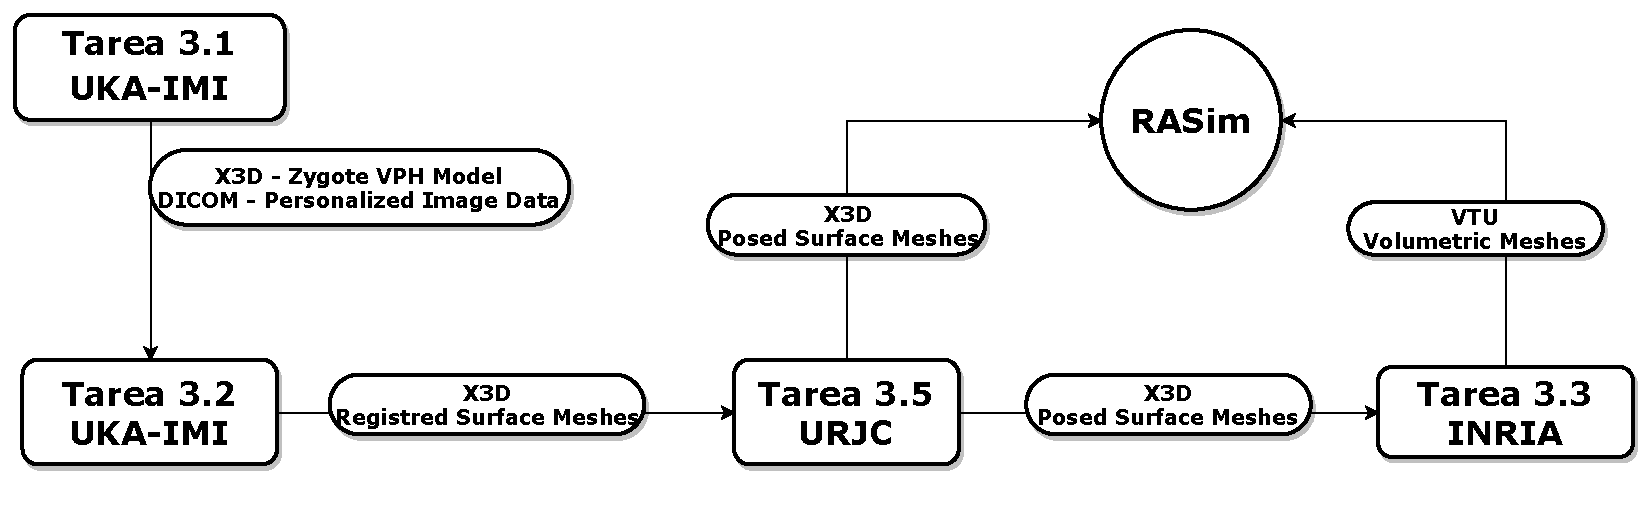
\includegraphics[width=1\textwidth]{IMG/DiagramaITGVPH.pdf}
    \caption{Arquitectura propuesta para la herramienta \acs{ITGVPH}. El formato de intercambio es \acs{X3D} y \acs{VTU}.}
    \label{fig:toolarq}
\end{figure}

Hay que destacar que no se integró  la tarea 3.4 (enumerada en la sección \ref{art:rasimas}) que se encargaba de la generación de la descripción fisiológica al no ser necesaria. Por parte de los socios médicos del proyecto, se decidió no incluir la simulación de la técnica de estimulación eléctrica del nervio en el simulador \ac{RASim} con el objetivo de  fomentar solo la práctica de la \ac{RA} guiada por \ac{US}.

El proceso comienza con el módulo de registro diseñado por \ac{UKA-IMI}. Se procede a cargar una imagen médica que contiene la anatomía objetivo, procedente de una base de datos que almacena diferentes imágenes médicas (el formato escogido es llamado \acs{DICOM}), además del modelo superficial anatómico de referencia en formato \ac{X3D}. Después, se realiza un registro automático entre la imagen médica y el modelo comercial, dando como resultado un nuevo modelo que será el primer paso para crear un \ac{VPH}. Para más información se puede consultar \cite{deOliveira:2015}. Este resultado será la entrada de la siguiente etapa.

En la segunda etapa se utiliza el módulo de posicionamiento. Esta etapa se corresponde al objetivo principal de esta tesis ampliamente descrito en el capítulo \ref{cap:posing}. Este recibe el modelo \ac{VPH} que contiene el modelo superficial y la anatomía interna, permitiendo a los usuarios seleccionar y generar posiciones útiles para el entrenamiento.

Finalmente, el modelo superficial resultante es suministrado al último módulo desarrollado por \ac{INRIA}. Esta tarea se encarga de generar el modelo volumétrico con  información biomecánica.
Tanto el modelo resultante superficial como el modelo volumétrico producidos por la herramienta \ac{ITGVPH}, se utilizarán por el simulador \ac{RASim}. Para más información se puede consultar \cite{ded3.3}.



%A continuación, se va a proceder a explicar cada etapa por separado.


% \subsubsection{Generación del modelo anatómico}
% Este módulo ha sido desarrollado por \ac{UKA-IMI} con el objetivo de realizar un registro entre las imágenes médicas y el modelo anatómico de referencia. Como se puede observar en la figura \ref{fig:r32}, el módulo ha sido divido en 5 tareas:
% %Deliverable D3.22:
% \begin{figure}[h]
%     \centering
%     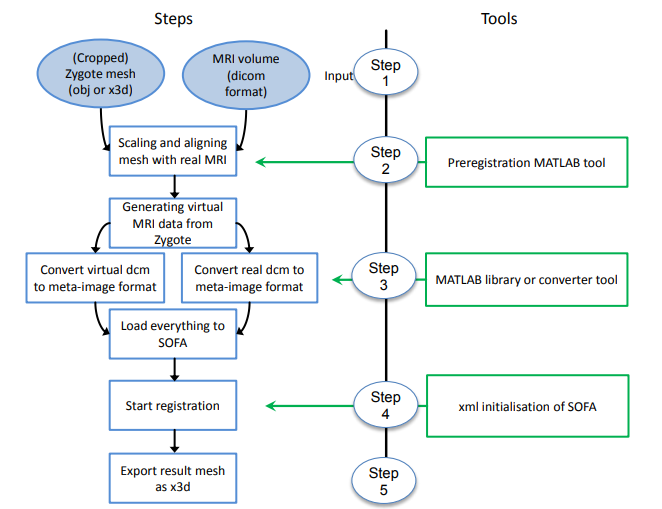
\includegraphics[width=0.5\textwidth]{IMG/rasimasd32.PNG}
%     \caption{ Diagrama de flujo de la herramienta de generación de modelo anatómico}
%     \label{fig:r32}
% \end{figure}
% \begin{enumerate}
%     \item  Se seleccionan los modelos de entrada (p. ej. \emph{ZygoteBody}$^{TM}$) e imágenes médicas (p. ej. \ac{IRM}) con los que se va a trabajar. Se procede a realizar un primer descarte de las estructuras anatómicas que se encuentran fuera de la región de interés de las imágenes médicas (por ejemplo, se eliminan brazos, cabeza, etc. si se va a trabajar sólo con la cadera).
%     \item Registro grueso: se procede a posicionar el modelo anatómico y las imágenes médicas en el mismo sistema de coordenadas y se crea el primer alineamiento (pre-registro) para prepararlo para el registro fino más adelante. Se procede a realizar un registro grueso utilizando \cite{antoinemri}. Esta técnica genera una imagen médica reconstruida para las dos representaciones e intenta ajustarlas para conseguir una alineación en cuanto a translación, rotación y escalado.
%     \item Conversión de formatos: se procede a convertir ambos modelos a una imagen 3D que es capaz de leer el software \ac{SOFA}, que será el encargado de realizar la siguiente etapa.
%     \item Registro fino: utilizando la técnica desarrollada en \cite{gilles2008}, se realiza un registro que permite deformaciones plásticas y elásticas entre dos modelos.
%     \item Por último, el modelo final se convierte al formato de intercambio para la herramienta.
% \end{enumerate}

% %%%%%%%%%%%%%%%%%%
% \subsubsection{Posicionamiento del paciente}
% Esta herramienta ya ha sido ampliamente descrita en la sección \ref{rasim:posing}. 
% No obstante, ha sido necesario realizar unas modificaciones adicionales para poder incorporar el algoritmo propuesto, a esta herramienta.


% \subsubsection{Generación del modelo volumétrico}

% Este módulo tiene como objetivo generar una malla volumétrica con los parámetros biomecánicos usados por el simulador \ac{RASim}. Desarrollado por \ac{INRIA}, se componen de los siguientes pasos:
% \begin{enumerate}
%     \item Se crea una imagen 3D basada en \emph{vóxeles} al igual que el proceso de volumetrización explicado en la sección \ref{posing:volumetrizacion}. Se etiqueta cada \emph{vóxel} con el tejido al que corresponde y así poder generar una imagen volumétrica que contenga todos los tejidos.
% \item En esta etapa se genera una malla de tetraedros a partir de la imagen 3D de la etapa anterior. Para ello, se utiliza la librería \ac{CGAL}.
% Para cada dominio (todos aquellos \emph{vóxeles} con la misma etiqueta) el algoritmo determina un conjunto optimizado de tetraedros que cumpla con los parámetros (ver anexo \ref{anexo:criterios}).  
% La malla generada es exportada al formato \ac{VTU} que contendrá toda la información necesaria para la simulación.
% Además, se incorpora información adicional que permita al núcleo de simulación calcular ciertos comportamientos. Por ejemplo, los vértices que están en contacto con un tejido óseo son marcados para que en el simulador \ac{RASim} pueda interpretarlos y generar una respuesta háptica al módulo de inserción de aguja.

% \end{enumerate}

Es importante destacar que, aunque las tres etapas crean modelos volumétricos del mismo modelo anatómico, la finalidad de cada uno es diferente y los parámetros difieren según el objetivo de este, por lo que no pueden ser compartidos. El detalle y las dimensiones que se consiguen en el módulo de posicionamiento \ac{TPTVPH} son muy superiores a las recomendadas como salida de la tercera etapa, ya que no se van a ejecutar simulaciones físicas sobre esa malla. Además, también se tiene en cuenta el objetivo de que las tareas puedan ser omitidas individualmente y tratadas como cajas negras para no compartir nada más que los datos necesarios para llegar al resultado final.



% \subsection{Interfaz de usuario}
% \label{rasim:herramientaui}

\begin{figure}[htbp]
    \centering
    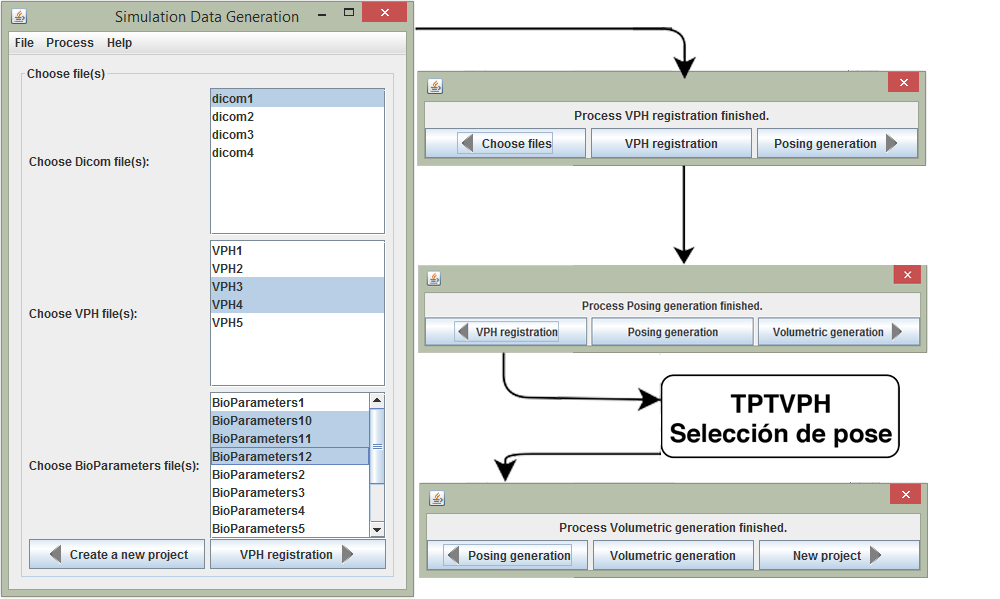
\includegraphics[width=0.8\textwidth]{IMG/toolkitui.png}
    \caption{Interfaz de la herramienta \acs{ITGVPH}. El usuario elegirá los modelos con los que quiere trabajar. Avanzará en el proceso hasta que la herramienta \acs{TPTVPH} le pregunte por la selección de pose. Una vez terminado, la herramienta sigue con el proceso.}
    \label{fig:toolui}
\end{figure}


%A continuación, se muestra la interfaz desarrollada para la herramienta \ac{ITGVPH}.
La interfaz ha sido diseñada para tener la mínima complejidad, debido a que se pretende reducir la dificultad para usuarios sin perfil técnico. De esta manera, la interfaz de la herramienta se puede resumir en la figura \ref{fig:toolui}. En esta figura se puede observar que en la primera ventana se pueden seleccionar todos los parámetros necesarios para que la herramienta trabaje de forma automática.
En orden, el primer parámetro que se puede seleccionar es el conjunto de imágenes médicas que están disponibles. Como se muestra en la figura, en este caso se disponen de imágenes en formato \acs{DICOM}.
Seguidamente, el segundo parámetro es el modelo anatómico de referencia que se pretende usar, como puede ser \emph{ZygoteBody}$^{TM}$ o \emph{Anatomium}. En los primeros prototipos sólo se ha utilizado el modelo anatómico \emph{ZygoteBody}$^{TM}$ pero la herramienta está diseñada para permitir la entrada de cualquier modelo anatómico de referencia. Este modelo será usado para hacer un registro con las imágenes anteriormente seleccionadas. 
Finalmente, se selecciona el archivo que contiene los parámetros biomecánicos y que se utilizarán en la última etapa.



Una vez están los ficheros seleccionados, el usuario sólo tendrá que avanzar a través de los menús contextuales para seguir avanzando en el proceso. Después de la fase de registro y generación del \ac{VPH}, se lanzará la interfaz de la herramienta \ac{TPTVPH} para que el usuario seleccione la postura del modelo anatómico. Una vez guardada, la herramienta seguirá con la siguiente tarea.



\section{RASim}
\label{rasim:rasim}
El simulador \ac{RASim} proporciona el entorno de trabajo para el entrenamiento de la \ac{RA}.  
Los \ac{WP} 4 y 5 definen todas las tareas para el desarrollo de los prototipos \ac{RASim} y \ac{RAAs}. Las tareas del 1 al 4 del \ac{WP} 4 corresponden a los módulos por separado de \ac{RASim} y las tareas 1 y 2 del \ac{WP} 5 corresponden a su integración en el prototipo. 
La responsabilidad del primer prototipo de \ac{RASim} recae en el equipo de trabajo de \ac{SG}, siendo cada módulo desarrollado por diferentes integrantes del proyecto. Aun así, la comunicación entre los diferentes grupos ha sido fundamental para conseguir una buena cohesión de todos los elementos del simulador. En esta tesis, se ha contribuido al simulador con el módulo de \ac{Courseware}. Este módulo se encarga del entrenamiento y gestiona los componentes del simulador. Por tanto, se trabajó conjuntamente con los demás participantes de \ac{RASimAs} en la construcción del prototipo \ac{RASim}.


%El objetivo era realizar un entorno de trabajo que permite al usuario entrenar el procedimiento de la forma más parecida a la situación real que se encontrarán en su futuro profesional.

% \subsection{Caso de uso}
% \label{rasim:casodeusorasim}

 

%Por ello el usuario, normalmente estudiante de anestesiología, se sentará delante del entorno de trabajo y se identificará en el sistema para poder almacenar y seguir su evolución durante todo el proceso. En las primeras sesiones, el usuario podrá revisar contenido multimedia para familiarizarse con el simulador y el procedimiento médico. El siguiente paso, será realizar una sesión guiada \del{en la cual} que  consiste en que el simulador va orientando al usuario en todos los pasos que debe realizar para completar con éxito el procedimiento médico. Durante el proceso, el usuario recibirá retroalimentación formativa por los errores o aciertos cometidos. Al finalizar la sesión, el simulador mostrará una retroalimentación sumativa sobre el desempeño del usuario y métricas recogidas por el simulador. Cada estudiante tiene designado un tiempo y objetivos mínimos que deberá cumplir antes de continuar con el entrenamiento. Una vez completada la primera sesión guiada, el usuario podrá repetir la sesión guiada o realizar una sesión libre, en la que el simulador no proporcionará ninguna indicación y sólo se recogerán métricas de la sesión. Todas las evaluaciones y métrica serán enviadas a un servidor dónde el supervisor podrá consultar y revisar la evolución de los usuarios.

El simulador consta de una mesa de trabajo donde se situarán todos los periféricos con los que interaccionará el usuario. En la mesa se encontrarán dos monitores para mostrar la escena virtual y la imagen de \ac{US}, junto con los dispositivos que simulan una sonda de ultrasonidos (\emph{\acs{tracker}}) y una aguja (dispositivo háptico). En cuanto al software, en la figura \ref{fig:coursearq} se puede observar la arquitectura software propuesta para el simulador: 
\begin{itemize}

    \item Módulo US: se encarga de simular el proceso de generación de la imagen \ac{US}.
    \item \acs{SOFA}: es el módulo encargado de la simulación física.
    \item \emph{H3D}: es un módulo de visualización de la escena virtual y comunicación con los dispositivos.
    \item \acs{Courseware}: es la plataforma de aprendizaje que se comunica con el módulo \emph{H3D}, \ac{US} y el servidor local .
    \item Servidor local y global: es un módulo para almacenar y gestionar la información del simulador.
\end{itemize}

\begin{figure}[ht]
    \centering
    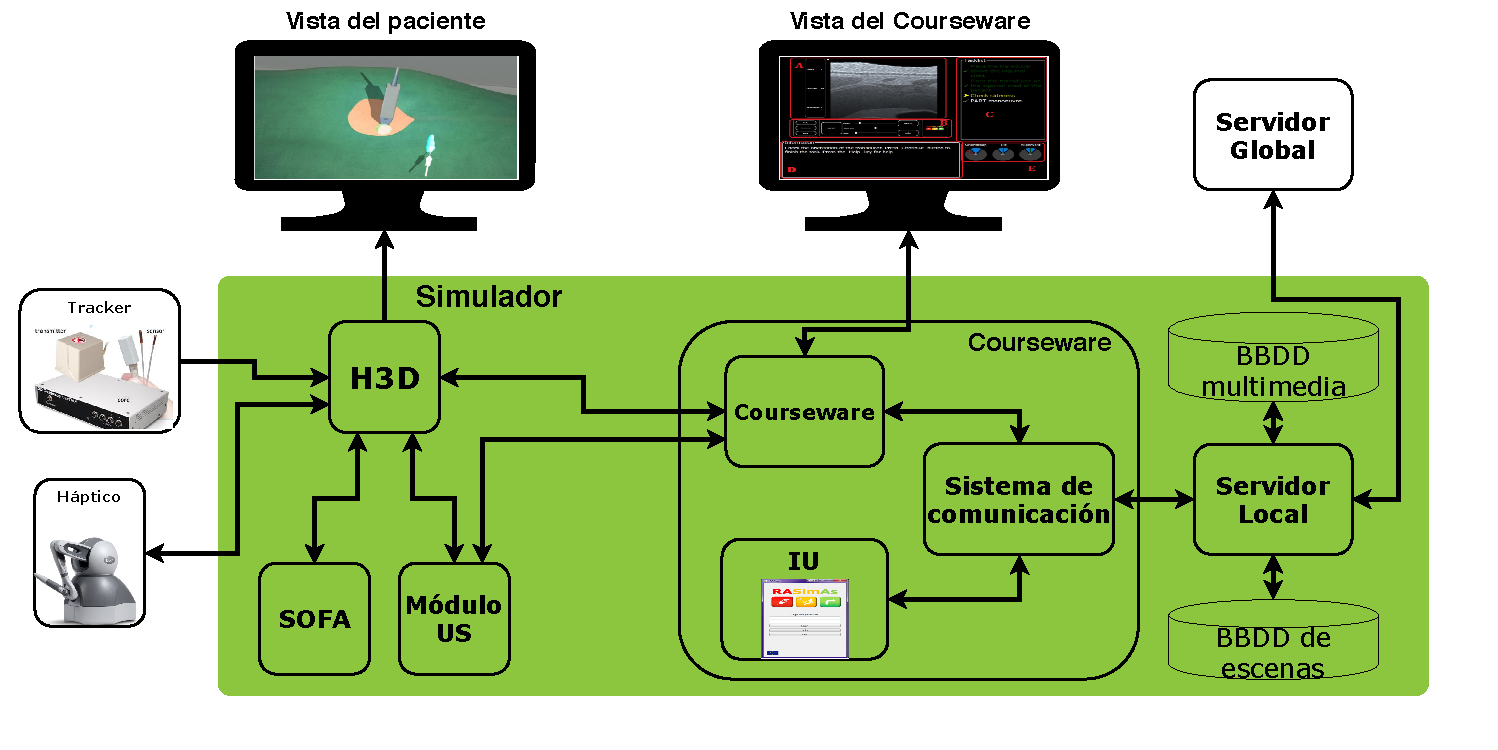
\includegraphics[width=\textwidth]{IMG/RasimArq.pdf}
    \caption{Descripción inicial de la arquitectura de \acs{RASim}.}
    \label{fig:coursearq}
\end{figure}
%\todo{rehago la imagen supongo}


A continuación se describirán brevemente los distintos componentes del simulador.



%Estos dispositivos están conectados a un computador. El computador centraliza el software desarrollado y la interacción con el usuario. A través de dos monitores se mostrará al usuario información visual y a través de un dispositivo háptico se proporcionará respuesta táctil. Además, se incorporará un \ac{Courseware}\footnote{Término ampliamente utilizado en la industria } que servirá para proporcionar una plataforma de aprendizaje y autoevaluación. Al mismo tiempo, esta herramienta puede recopilar métricas y mostrar información útil al usuario. Esta aplicación será la encargada de cargar diferentes escenarios, guardar sesiones de entrenamiento, mostrar tareas y lecciones específicas del entrenamiento.

%El prototipo creado tendrá que ser evaluado como parte del proyecto europeo en estudios clínicos controlados dirigido tanto a expertos como estudiantes de anestesiología. Antes de alcanzar los experimentos clínicos, cada módulo del simulador debe ser probado por separado (\ac{WP}4 sección \ref{art:rasimas}) para asegurar el proceso de evaluación y permitir un desarrollo iterativo con el objetivo de construir un prototipo validado y fiable (\ac{WP}5 sección \ref{art:rasimas}). 

% Para cumplir con ello se han propuesto las siguientes especificaciones para el simulador:

% \begin{itemize}
%     \item Computador: el sistema donde se ejecutará el sistema deberá ser lo suficiente potente como para ejecutar simulaciones físicas que permiten simular el comportamiento de los tejidos, calcular la retroalimentación háptica y generar la representación visual sin que afecte a la interactividad del usuario.
%     \item Plataforma de trabajo: para estandarizar el entorno de trabajo se ha diseñado una plataforma que permite conocer la disposición tanto del maniquí como de los dispositivos \ac{E/S} con el objetivo de ser fácilmente reproducible en diferentes instituciones. Deberá estar diseñado para personas diestras y zurdas.
%     \item Maniquí y región de interés: con el objetivo de proporcionar el mayor realismo posible, se ha propuesto incluir un maniquí en la plataforma para que el usuario interactúe sobre un espacio de trabajo controlado.
%     \item Monitores: es necesario mostrar información visual sobre la habitación virtual y la imagen de \ac{US}. Además, se mostrará información útil para el aprendizaje.
%     \item Sonda de ultrasonidos: es uno de los instrumentos principales de la \ac{RA}, por ello conviene que la sonda sea lo más realista posible.
%     \item Aguja: instrumento fundamental en el procedimiento. Al ser una parte importante del entrenamiento, el simulador captura su movimiento y posición y devuelve fuerzas que simularan las sensaciones para el usuario como si fuera en un entorno real.
%     \item \ac{Courseware}: una aplicación que permita integrar todos los elementos del sistema además de proporcionar un sistema de entrenamiento y evaluación.
% \end{itemize}



\subsection{Hardware}


\subsubsection{Mesa de trabajo}

El principal objetivo de crear una mesa de trabajo es estandarizar la posición relativa de los dispositivos anteriormente citados. %Además de suplir las carencias de estos para mejorar la inmersión del usuario en el simulador.
Se ha diseñado una plataforma en forma de "T" para poder incorporar de manera perpendicular el campo de trabajo del dispositivo magnético por una parte y el dispositivo háptico por otra. De esta manera, el dispositivo háptico puede ser intercambiado de posición para permitir que el simulador pueda ser configurado para que se pueda realizar con ambas manos. Situado en el centro, se colocará un maniquí de un material deformable para simular la zona anatómica del paciente. 

Junto con la plataforma, se encuentran los monitores situados de manera frontal. Esto hace que el usuario tenga todos los elementos en su rango de visión y evite realizar una rotación de cuello. En el primero, se muestra la vista del paciente que consiste en la \emph{renderización} de la escena virtual dónde se encuentra el modelo anatómico de un paciente y una representación virtual de los instrumentos médicos. Además, esta vista se puede utilizar para añadir elementos virtuales que mejoren la efectividad del entrenamiento. 
Por otra parte, en el segundo monitor se muestra el software de entrenamiento en el que se incluye la imagen de \ac{US}. Una versión del prototipo se puede ver en la figura \ref{fig:simulator}.


\begin{figure}[ht]
    \centering
    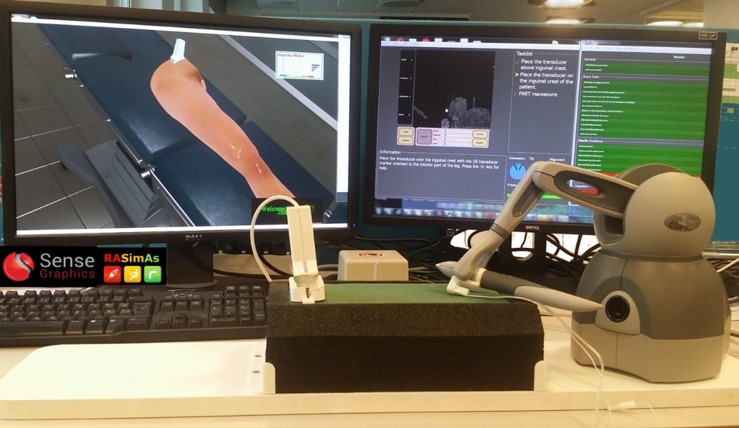
\includegraphics[width=0.95\textwidth]{IMG/simulator.jpg}
    \caption{Diseño de la mesa de trabajo. El rectángulo de espuma se sitúa en el centro. A continuación, el emisor del dispositivo magnético, y los monitores. A los laterales, el dispositivo háptico puede ser intercambiado de posición.}
    \label{fig:simulator}
\end{figure}


\subsubsection{Maniquí} 
En el procedimiento de \ac{RA}, el radiólogo apoya la sonda de ultrasonidos y parte del brazo en la anatomía del paciente. Por tanto, es necesario reproducir la zona anatómica que ayudará al usuario a apoyar la sonda de ultrasonidos e introducir la aguja en algún lugar de manera segura y controlada. Esto requiere que el material sea resistente tanto a presión como a la inserción de la aguja repetidamente sin introducir fuerzas adicionales al sistema. Por tanto, se diseñó un rectángulo de espuma de poliuretano que sirviera de recipiente para un relleno con espuma floral como se puede observar en la figura \ref{fig:simulator}.

% La idea original era obtener un reemplazo rápido porque la espuma floral, aunque permitía una inserción de la aguja sin apenas resistencia, era muy débil ante presión y rotaciones de la aguja. Además, las inserciones continuas debilitaban el material y pueden dar información a los usuarios que utilicen el simulador posteriormente.
% Para añadir consistencia a la espuma floral se ideó añadir una capa de silicona por encima. Esta capa permitía que la espuma no se deshiciera con el rozamiento y además proporcionaba cierta estabilidad, pero a la vez introducía un pequeño rozamiento que habría que salvar al introducir una aguja. En la figura \ref{fig:silicona} se puede observar un prototipo.

% \begin{figure}[ht]
%     \centering
%     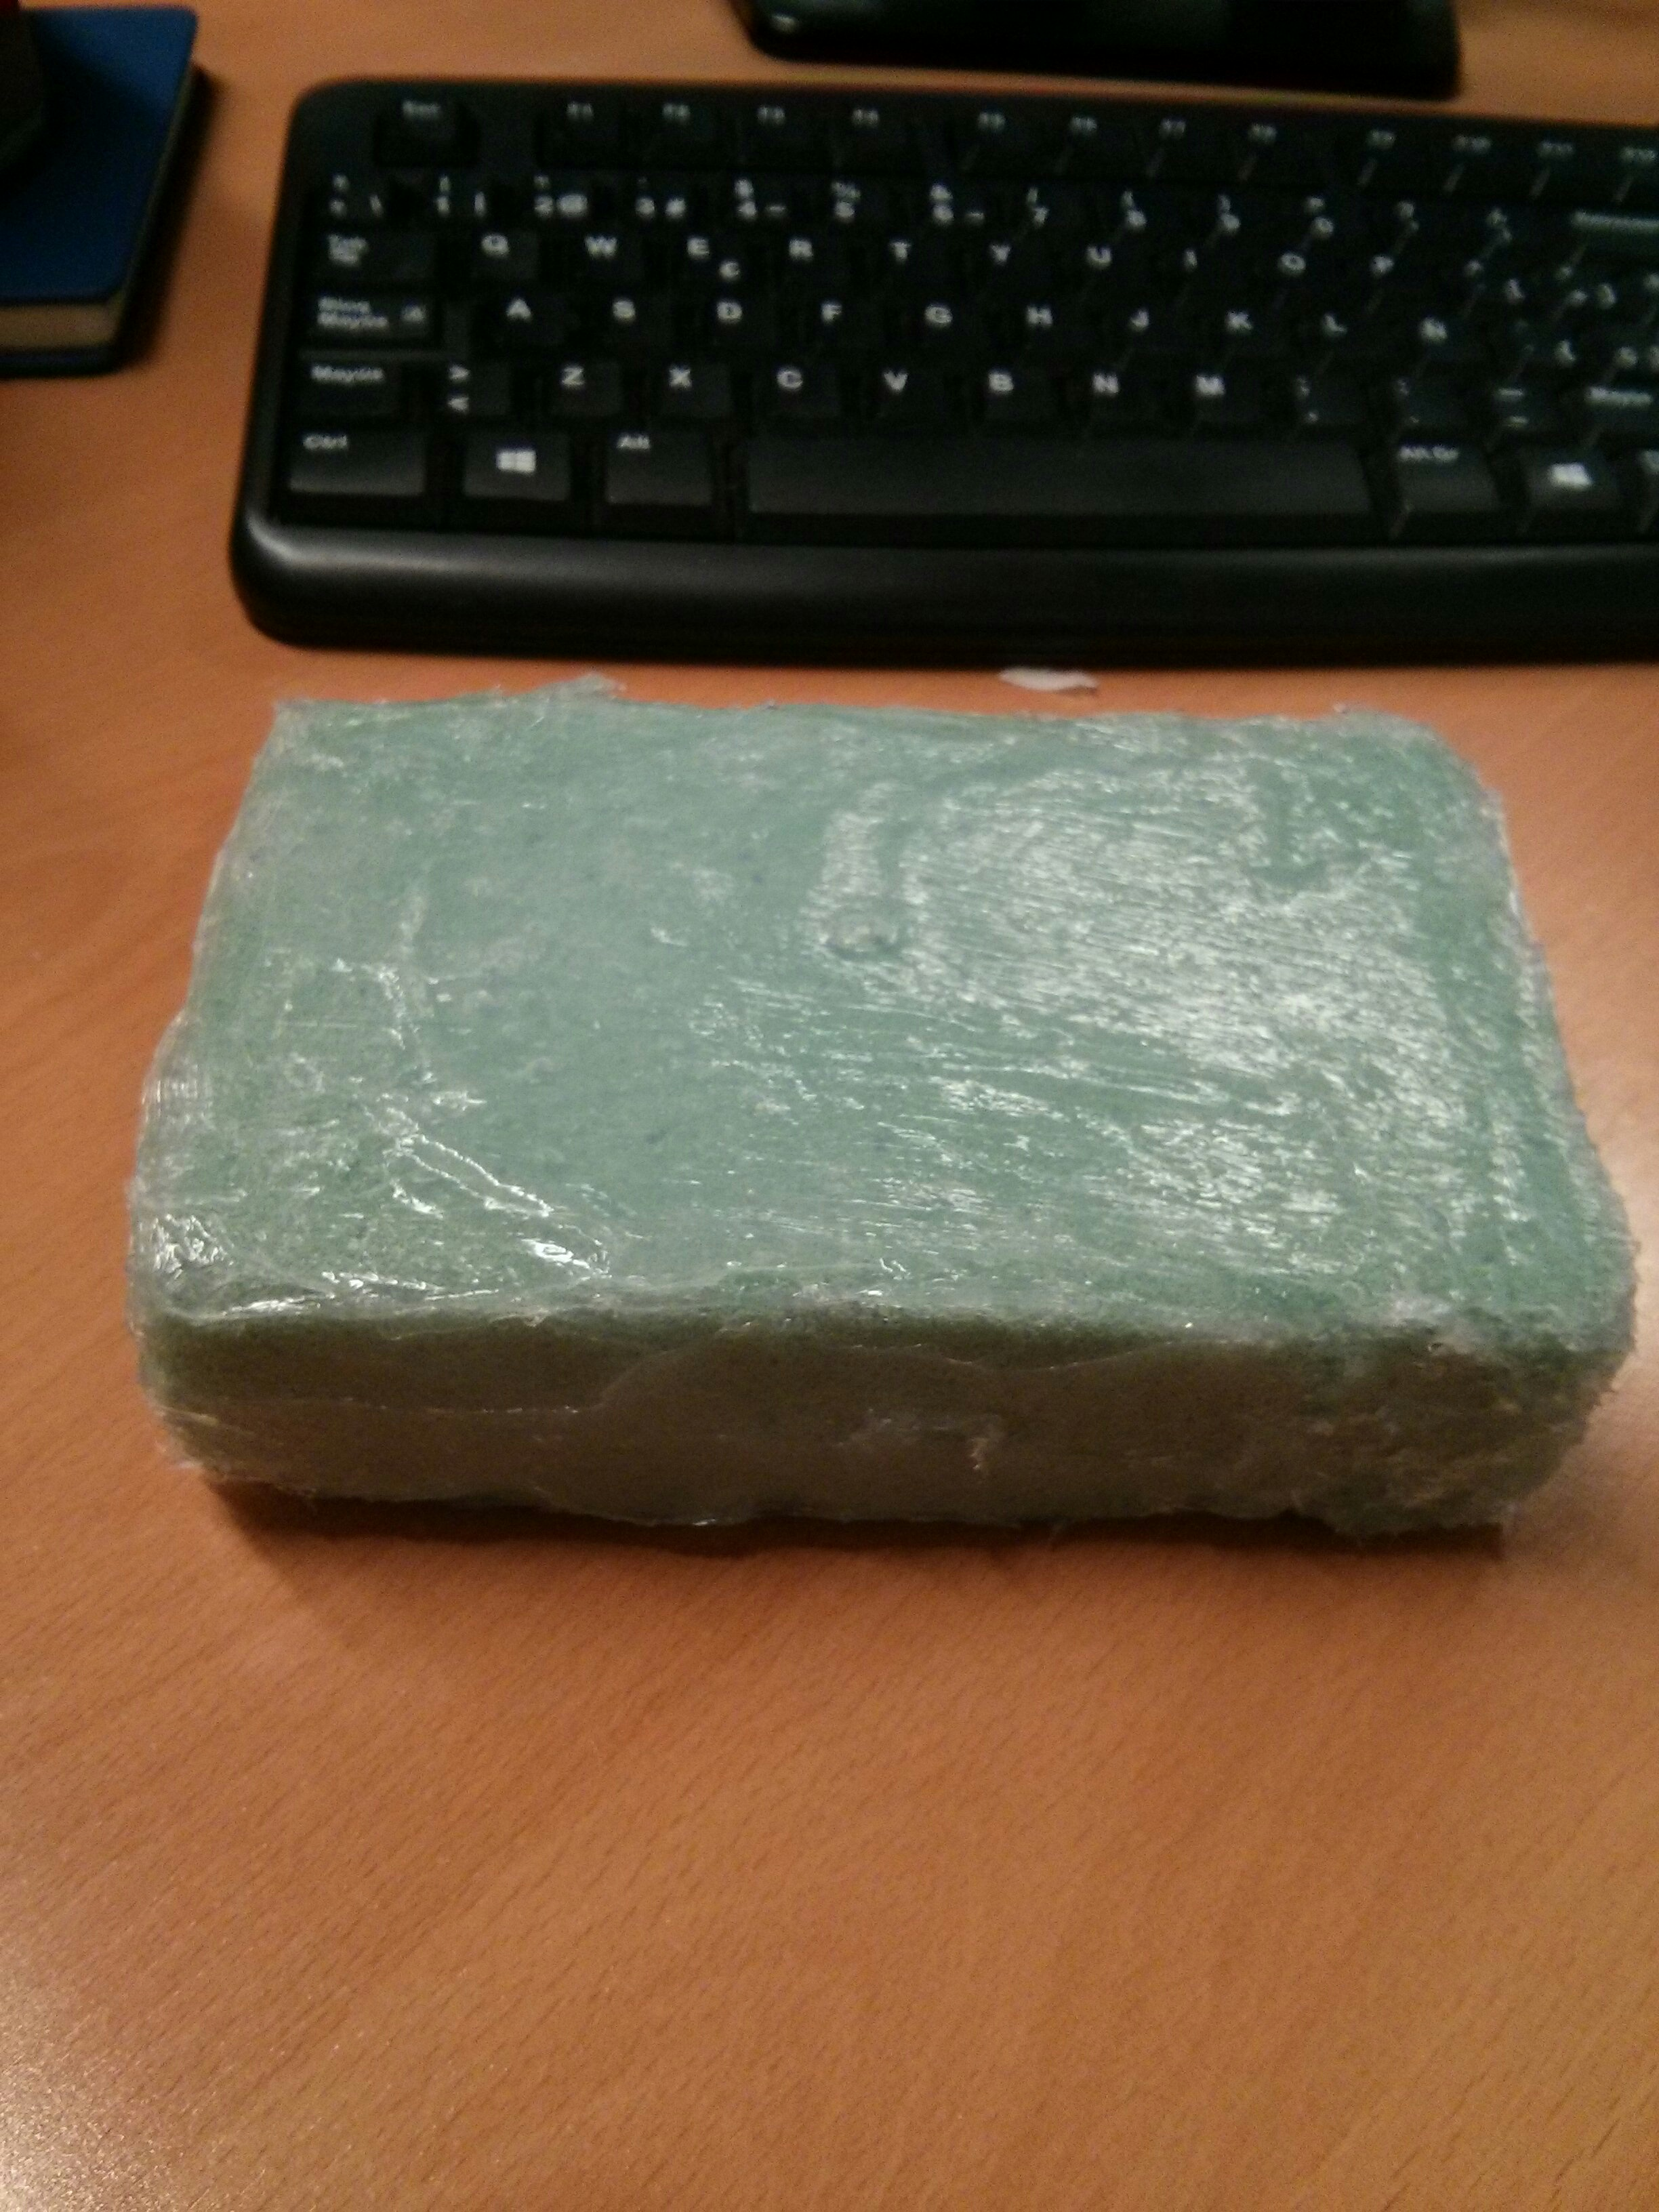
\includegraphics[width=0.5\textwidth]{IMG/silicona.jpg}
%     \caption{Espuma floral cubierta de una capa de silicona para mejorar su consistencia.}
%     \label{fig:silicona}
% \end{figure}

% Desde la \ac{URJC} se propuso utilizar otro material que no implique un bloque de espuma. Existe un material arenoso que intenta simular un fluido \emph{no newtoniano} (ver figura: \ref{fig:arena}) de tal forma que es resistente a la presión y rozamiento de la sonda, pero permite una inserción de la aguja sin apenas resistencia. Además, al ser un material con características parecidas a las de un fluido, las continuas inserciones no debilitan el material. Puede ser fácilmente reemplazable y su coste es pequeño.


% \begin{figure}[ht]
%     \centering
%     \includegraphics[width=0.5\textwidth]{IMG/arena.jpg}
%     \caption{Arena \emph{kinética}}
%     \label{fig:arena}
% \end{figure}
% \todo{rehacer figura arena}

% Existen otros problemas al restringir el espacio de trabajo a un rectángulo de espuma o arena. Este rectángulo no representa fielmente el modelo anatómico. Al no ser iguales que el modelo del paciente virtual, esto generaba inconsistencias entre el mundo virtual y el real que afectaba a la realización correcta del procedimiento.
% Actualmente, la tecnología de impresión 3D permite una solución rápida y barata para fabricar modelos personalizados. Con el objetivo de mejorar el realismo de la aplicación, se ha diseñado el rectángulo contenedor que tuviera la forma anatómica utilizando el mismo modelo que se usaría en el simulador. Solo haría falta introducir y adaptar la espuma o arena en el interior de este modelo. Esto permitiría utilizar la forma anatómica como se puede observar en la figura \ref{fig:pierna}. 

% \begin{figure}[ht]
%     \centering
%     \includegraphics[width=0.5\textwidth]{IMG/pierna.PNG}
%     \caption{Versión del contenedor de la espuma con forma de pierna.}
%     \label{fig:pierna}
% \end{figure}

% Aun así, esta solución depende enormemente del modelo anatómico que se esta simulando y necesitaría imprimir un soporte para cada modelo virtual que se utilizará en el simulador. 



% \subsubsection{Monitores}

% Una característica importante de una herramienta de \ac{RV} es la inmersión del usuario en el sistema. Esta inmersión está normalmente muy influenciada por los dispositivos de entrada y salida que le conecta con el motor de \ac{RV}. Cuanto más se asemejen a la realidad, proporcionarán una sensación de inmersión y presencia que ayudará al usuario a mejorar su experiencia en el sistema y por tanto, el objetivo que hubiera detrás de éste (entrenamiento, preparación, etc...). Normalmente, como se ha introducido en el capítulo \ref{cap:intro}, estos dispositivos están orientados a determinados canales sensoriales. En este sistema, sólo se ha considerado el canal visual y el táctil debido a que el procedimiento de \ac{RA} no implica otro tipo de sentidos. A continuación, se hará una descripción de los dispositivos que componen el prototipo desarrollado en el proyecto.


% \paragraph{Vistas del paciente y del ecógrafo}\mbox{}\\

% La vista es el sentido de entrada dominante en muchos aspectos cotidianos y en este simulador, concretamente, es necesario que el usuario pueda situar los instrumentos médicos en relación con la anatomía del paciente. Además, necesita recabar toda la información posible de los tejidos internos que le proporciona la imagen de ultrasonidos y no puede observarse a simple vista. Por tanto, el usuario utiliza su capacidad visual para colocar los instrumentos médicos en la posición requerida y a la vez requiere del ecógrafo para su correcto desempeño.

% Para representar la vista del paciente y de la máquina de ultrasonidos, se ha incorporado dos pantallas al entorno de trabajo del simulador. 
% En uno de ellos se muestra la vista del paciente. Esta consiste en la \emph{renderización} de la escena virtual dónde se encuentra el modelo anatómico de un paciente y una representación virtual de los instrumentos médicos. Además, esta vista se puede utilizar para añadir elementos virtuales que mejoren la efectividad del entrenamiento. 
% Por otra parte, en el otro monitor se utiliza para mostrar el software de entrenamiento que incluye la imagen de ultrasonidos generada por el motor de \ac{RV}.

\subsubsection{Sonda de ultrasonidos}

El posicionamiento de la sonda de ultrasonidos es clave en el procedimiento de \ac{RA}. La técnica eco-gráfica es fundamental para encontrar el nervio a anestesiar. Con el objetivo de simular este aparato médico, se ha diseñado un modelo impreso en 3D que imita una sonda real que envuelve al sensor del dispositivo de seguimiento. Para esta finalidad, se ha utilizado un \emph{\acs{tracker}} magnético\footnote{Ascension 3D-Guidance trakSTAR, módelo 800 \cite{Ascension}.} como se puede observar en la figura \ref{fig:simulator}. 
%Este dispositivo es capaz de saber la posición de un receptor o sensor gracias a la generación de un campo magnético producido por un emisor. La deformación del campo magnético producido por el receptor ayuda al dispositivo a conocer su posición y orientación. Este sensor es el que se introduce dentro del modelo impreso y sirve para saber la posición de la sonda respecto a la mesa de trabajo. %De esta manera el usuario utiliza un instrumento parecido lo más posible a uno real.

% \begin{figure}[ht]
%     \centering
%     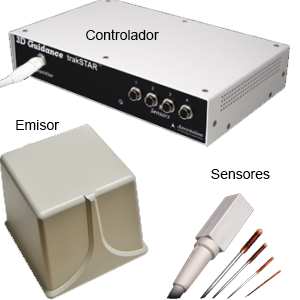
\includegraphics[scale=0.65]{IMG/tracker.png}
%     \caption{\emph{Ascension 3D-Guidance trakSTAR, módelo 800} \cite{Ascension} utilizado en \ac{RASim}}
%     \label{fig:tracker}
% \end{figure}

% En un principio, el diseño del modelo 3D intenta recrear la sonda original a la vez que se incluye el dispositivo de seguimiento dentro de él. Se ha diseñado un modelo compuesto por dos piezas que en el interior acoge el sensor sin que el usuario sea consciente (ver figura \ref{fig:m3d}). Además, el propio cable del sensor es similar al cable que se encontrarán los usuarios en un entorno real.

% \begin{figure}[ht]
%     \centering
%     \includegraphics[width=0.5\textwidth]{IMG/modelo3d.png}
%     \caption{Primer prototipo del modelo impreso de la sonda de ultrasonidos para alojar el sensor del \emph{tracker} magnético.}
%     \label{fig:m3d}
% \end{figure}

% Debido a limitaciones de hardware de poder recrear fielmente la deformación de los tejidos de la piel cuando el médico presiona la sonda contra ella, se decidió junto con los profesionales médicos del proyecto que habría que incorporar algún mecanismo que ofreciera al usuario una sensación de elasticidad de la piel. Así de esta manera, se ideó una pieza adicional conectada al modelo 3D a través de un muelle que permitía la sensación de tejido flexible al usuario como se puede observar en la figura \ref{fig:m3dv2}.

% \begin{figure}[ht]
%     \centering
%     \includegraphics[width=0.5\textwidth]{IMG/modelo3dv2.jpg}
%     \caption{Modelo impreso de la sonda de ultrasonidos con la actualización que permite tener sensación de elasticidad de la piel }
%     \label{fig:m3dv2}
% \end{figure}


\subsubsection{Aguja}
\label{rasim:aguja}
En el procedimiento de \ac{RA} guiado por \ac{US}, el primer paso es la localización del nervio. Una vez localizado, la inserción de la aguja y su aproximación al nervio que se va a anestesiar es otro punto crucial del procedimiento. El médico debe introducir la aguja en una posición relativa a la sonda, por tanto, es necesario que el usuario practique con los dispositivos. Se mueve la sonda y cuando el usuario tiene el nervio localizado, se introduce la aguja de forma segura en el maniquí. El simulador debe interpretar la inserción de la aguja y devolver las fuerzas correspondientes a atravesar las fascias que se encuentran en la anatomía. 

%El medico utiliza el taco para saber donde esta la aguja. Siempre que se traviesan las fascias el lo siente.

La inserción real de la aguja implica que su movimiento pueda definirse a través de 5 \ac{DOF}. La correcta posición, el movimiento adecuado y la sensación de la aguja son muy importantes en el entrenamiento de los nuevos médicos. Por ello la selección del dispositivo con el que replicar estos comportamientos no es sencillo. Los \emph{\acs{tracker}s} magnéticos anteriormente citados serían una buena solución debido a que son capaces de registrar el movimiento del sensor en sus 6 \ac{DOF}, pero estos dispositivos no están pensados para devolver fuerzas al usuario. Los dispositivos hápticos suelen resolver este tipo de problemas al ser utilizados como dispositivos de seguimiento y a la vez son capaces de reproducir fuerzas e interaccionar con el usuario.

Desde el proyecto \ac{RASimAs} se ha seleccionado el dispositivo \emph{Touch} de la empresa \emph{3D System}\cite{touch} (ver figura \ref{fig:simulator}). Aunque este dispositivo solo sea capaz de proporcionar fuerzas en los 3 \ac{DOF} básicos (X,Y,Z), se ha de alcanzar un compromiso entre versatilidad y el presupuesto. Existen dispositivos hápticos que pueden ofrecer la experiencia de simular la inserción de una aguja, pero su complejidad implicaría un coste inasequible para la comercialización de un simulador. %y aumentaría la dificultad de una inmersión del usuario debido a que no existe dispositivo háptico con esas características de pequeñas dimensiones. Sin embargo, el dispositivo \emph{Touch} proporciona la posibilidad de que el sistema sea más barato y consiga cierto realismo. 
%El usuario maneja este dispositivo a través de una especie de bolígrafo (\emph{stylus}) que es capaz de reconocer la posición, orientación y devolver fuerzas. Incluso es lo suficiente ligero para poder permitir su colocación en otras posiciones con el objetivo de permitir a los usuarios elegir con que mano utilizar los dispositivos.

% Aun así, la utilización de este dispositivo para simular una aguja no esta exento de problemas. El objetivo es simular una aguja real pero el actuador del dispositivo es completamente diferente y sería muy difícil replicar el mismo comportamiento que se experimenta en una situación real.
% Con el objetivo de solventar este problema, se ha intentado adaptar el bolígrafo que dispone para que aloje una aguja real utilizado en el procedimiento.
% El dispositivo \emph{Touch} permite desmontar la punta del actuador con la intención de permitir a otros desarrolladores encajar nuevas creaciones a través de un conector tipo \emph{Jack}. En este caso, desde \ac{SG} se diseñó un modelo 3D que encaje en el conector de manera que la aguja pueda ser agarrada por el usuario. Esto permite que se puedan utilizar el mismo tipo de aguja estandarizando la solución como se puede ver en la figura \ref{fig:needle}.

% \begin{figure}[ht]
%     \centering
%     \includegraphics[width=0.5\textwidth]{IMG/needle.PNG}
%     \caption{Primer prototipo para adjuntar una aguja real al dispositivo háptico.}
%     \label{fig:needle}
% \end{figure}

% Esta solución, aunque bien diseñada, en las primeras pruebas mostró varios factores que hicieron descartarla por parte del comité médico. El desplazamiento entre el centro del conector del dispositivo háptico y el lugar donde el usuario agarraba la aguja junto con la flexibilidad de esta, introducía un desplazamiento virtual que hacía que el simulador no representará fielmente la posición real en el mundo virtual. Desde la \ac{URJC}, se sugirió una adaptación  anteriormente utilizada en un desarrollo anterior\cite{phantompen}. Esta versión encajaba en la forma de bolígrafo que tenía el dispositivo y permitía el uso de una aguja estandarizada de la misma manera como se puede apreciar en la figura \ref{fig:needle2}. Incluso, salvando las distancias, permite al usuario un agarre más realista. Esta versión fue la aceptada para el prototipo a falta de más soluciones y propuestas.


% \begin{figure}[ht]
%     \centering
%     \includegraphics[width=0.5\textwidth]{IMG/needle2.jpg}
%     \caption{Prototipo para permitir sujetar la aguja sin desplazamientos en el dispositivo háptico.}
%     \label{fig:needle2}
% \end{figure}
% \todo{rehacer la imagen de la aguja}



% Otro problema derivado de la selección del dispositivo era que el espacio de trabajo es limitado y cuanto más cerca se trabaja del límite de este espacio, más inestable puede ser el comportamiento del dispositivo. Afortunadamente el procedimiento de \ac{RA} tiene también un espacio limitado de acción y puede simplificarse la solución a este problema. Se propuso crear una mesa de trabajo que limite la acción del usuario al área de interés. 

\subsection{Software}

%\subsubsection{Motor de \ac{RV}}

%Uno de los componentes principales de un simulador de \ac{RV} es el motor donde se producen todos los cálculos que permiten simular la escena virtual. 
%En el contexto de \ac{RASim}, es lógico que este simulador tenga un núcleo que realiza las simulaciones físicas y cálculos necesarios con el objetivo de comunicarse con los dispositivos de entrada y salida. Además, también es necesario un núcleo de simulación que proporcione las imágenes de \ac{US} para conseguir mostrar una simulación realista que pueda ayudar al usuario. Por último, el sistema también deberá \emph{renderizar} la escena con la información de los dispositivos para ayudar al usuario a que alcance mayor inmersión de la escena. 

Debido a que en el proyecto \ac{RASimAs} participan multitud de instituciones, los módulos encargados de cada tarea han sido desarrollados independientemente por cada participante y se presentarán en las siguientes secciones.


\subsubsection{Simulación visual}

\emph{H3D} \cite{sensegraphics2012open} es una librería de código abierto (\ac{GPL})  orientada a la utilización de hápticos en entornos 3D desarrollada por la empresa \emph{Sensegraphics}. 

El módulo \ac{Courseware} utiliza la librería \emph{H3D} como punto de comunicación entre el software y los dispositivos. De esta forma gestionará los demás componentes y dispositivos. A través de este software, también se recopilará la información de los dispositivos de entrada.
En cuanto el simulador es iniciado, \emph{H3D} se encarga de cargar la escena seleccionada utilizando el formato \ac{X3D}, inicia el módulo de simulación física y activa los dispositivos:  el dispositivo háptico y el \emph{\acs{tracker}}. La vista del paciente y la sala de operaciones es \emph{renderizada} por \emph{H3D} a través de su gestor de ventanas.
%Las simulaciones físicas y el cálculo de las deformaciones de los tejidos como consecuencia de la colisión de los instrumentos médicos serán calculadas en el siguiente componte del simulador.

\subsubsection{Simulación física}

En esta ocasión, es el software \emph{SOFA} \cite{sofaweb}, desarrollado por el grupo \ac{INRIA}, el encargado de realizar las simulaciones físicas. Esto permite simular la deformación de los tejidos al contacto de la sonda o la aguja, además de proporcionar la respuesta física a la aguja que será retransmitida al dispositivo háptico.

La librería \emph{SOFA} es código abierto (bajo licencia \ac{LGPL}) y dispone de multitud de métodos y algoritmos matemáticos usados en simulación como distintos \emph{solvers}\footnote{Herramienta matemática para resolver sistemas de ecuaciones lineales.}, modelos físicos como \ac{FEM} y detección de colisiones, simulación de tejidos rígidos o flexibles.

En \ac{RASim}, \emph{SOFA} realiza las siguientes tareas:
\begin{itemize}
    \item Deformación de la piel y otros tejidos producida por la interacción de los instrumentos médicos utilizando el método \ac{FEM} co-rotacional.
    \item La interacción con la aguja a través de diferentes tipos de tejidos, simulando la penetración en la piel y las fascias, además de la fricción de los demás tejidos \cite{needleinsertion}.
   %\item La contracción de los músculos con una respuesta física según sus propiedades mecánicas.
    
\end{itemize}

\subsubsection{Simulación de ultrasonidos} 

En cuanto a la simulación de la imagen de ultrasonidos, se utiliza una librería basada en \ac{ViSTA} desarrollada por el grupo \ac{RWTH}. \ac{ViSTA} es código abierto (bajo licencia \ac{LGPL}) y se utiliza para implementar el algoritmo con el que se simula la generación de imágenes de \ac{US}.

El módulo de ultrasonidos está desarrollado con un algoritmo basado en métodos acústicos geométricos \cite{Law2015}, el cual es clasificado como un enfoque \emph{generativo}. Pensando geométricamente, la onda de sonidos se puede aproximar a través de rayos que interaccionan con elementos de la escena, por consiguiente producen un reflejo del rayo refractado o dispersado. Estos rayos se definen por energía acústica, que puede ser absorbida o disipada durante la interacción con la escena. Esta energía es usada para calcular la intensidad de los ecos y en consecuencia la intensidad de los \emph{píxeles} que servirán para construir la imagen resultante.

Para alcanzar tiempos interactivos en presentar las imágenes de ultrasonidos, la mayor parte de los intensos cálculos y operaciones pesadas son realizadas durante un proceso previo. Específicamente, en esta etapa se genera: un campo acústico que define las propiedades del haz de la sonda y el transductor, las texturas tridimensionales que serán usadas para simular la dispersión del rayo y, además, las estructuras de datos auxiliares que ayudarán a acelerar el proceso de simulación.
De esta manera, cuando el objetivo sea tener una respuesta interactiva, sólo será necesaria la posición y orientación de la sonda virtual que se usará para calcular el origen y la dirección de los rayos acústicos. Estos rayos serán muestreados a través de la escena, estimando la energía reflejada y la distancia recorrida a través de los tejidos. Por otra parte, el remanente de energía transmitida, las absorciones y reflexiones se tienen en cuenta para generar la imagen final.





% \subsection{Arquitectura del simulador}
% \label{rasim:arqrasim}

% Antes de continuar, se va a presentar la arquitectura lógica del simulador para permitir al lector que tenga una visión completa del sistema en su conjunto.

% Siguiendo la arquitectura de un simulador de \ac{RV} tipo que se puede observar en la figura \ref{fig:RVarq}  en el capítulo \ref{art:simulador}, un simulador puede ser definido por una serie de componentes. El usuario utilizará los dispositivos de entrada y salida que se comunicarán con un motor de \ac{RV} que calcula todas simulaciones físicas y visuales según la escena virtual almacenada en la base de datos. El motor actualizará el estado de la simulación según las tareas que hayan sido programadas. A continuación se procede a explicar cada componente por separado. 


%A continuación, se va a proceder a describir aquellos dispositivos que utilizan el canal táctil. \todo{este párrafo va bien aquí?}


\subsubsection{Servidor local y global}

El proyecto \ac{RASimAs} contempla que se almacene toda aquella información generada en la realización del proyecto. En cuanto a la información relevante para el simulador \ac{RASim}, se guardarán las escenas y modelos anatómicos que se utilizarán en el simulador. También, se almacenará el material multimedia complementario que sea necesario para la plataforma de entrenamiento. Además, esta base de datos servirá para guardar el perfil de los usuarios y las métricas que se recogerán para evaluarlos posteriormente.

Con el objetivo de no necesitar estar conectado a Internet permanentemente, se han diseñado un servidor local y otro global. El servidor local será instalado en el simulador de tal forma que periódicamente consulte nuevas actualizaciones o mande información al servidor global que comparten todos los simuladores.

\subsubsection{Courseware}

%Con el objetivo de mostrar la versatilidad y comprobar la hipótesis de esta tesis, se ha contribuido al proyecto \ac{RASimAs} con la generación de un módulo de entrenamiento que permita utilizar los modelos generados por el algoritmo de posicionamiento de pacientes virtuales. El desarrollo de este módulo y su posterior evaluación demostraría la capacidad del algoritmo propuesto en un ejemplo de caso de uso.

%Tanto el motor de \ac{RV} como los dispositivos de entrada y salida no podrían ser capaces de servir como herramienta de aprendizaje por si mismos si no hubiera un software que guía las tareas y las acciones del usuario cuando utiliza el simulador.
El módulo de \ac{Courseware} es una pieza fundamental en \ac{RASim} ya que gestiona la comunicación entre componentes, ayuda y recopila información de los usuarios. Se encarga de recopilar información de los dispositivos y se comunica con la base de datos que almacena las métricas de los usuarios. A la vez, será la aplicación encargada de manejar las ventanas y la interacción del usuario con el sistema. 

El usuario podrá identificarse en el simulador a través de una interfaz. La aplicación recibirá el perfil desde el servidor y basándose en el perfil del usuario, el \ac{Courseware} proporcionará el escenario de entrenamiento según el protocolo que se haya definido. Este módulo, es el encargado incluso de descargar nuevos escenarios del simulador desde el servidor. 

Debido a la complejidad e importancia de este módulo, será descrito en una sección independiente a continuación.


\section{Courseware}
\label{rasim:courseware}
%\todo{Introducir esto como contribución}
Todos los elementos anteriormente citados conforman un simulador de \ac{RV} por si mismo, pero no conforman una herramienta de entrenamiento sin un software que oriente al usuario en el proceso de aprendizaje. Por tanto, en el contexto de esta tesis, se ha contribuido en la creación del módulo \ac{Courseware}, que gestiona todos los componentes del simulador y se encarga de implementar todas las tareas relacionadas con el entrenamiento. El software se ha diseñado con la finalidad de ser la interfaz del simulador para ayudar al usuario a interaccionar con él. A su vez, este módulo proporciona una evaluación formativa y sumativa al usuario para mejorar el aprendizaje.

%De esta forma, el \ac{Courseware} es el encargado de permitir al usuario identificarse y comunicarse con el servidor. En el servidor se almacenan los materiales multimedia y los escenarios que se cargarán en el simulador. La aplicación también es la encargada de inicializar el motor de \ac{RV} con los módulos de simulación. También es el encargado de presentar la interfaz gráfica que se mostrará a través de los monitores. Por una parte, mostrará la vista de paciente, y por otra la vista del \ac{Courseware}. Esta ventana contendrá a su vez la información del simulador de ultrasonidos y todos los botones y la información adicional asociada al modo de simulación que se esté ejecutando.

%Este software permitirá comprobar si la herramienta de generación de \ac{VPH}, y por tanto la herramienta \ac{TPTVPH}, es útil para entrenar el procedimiento de \ac{RA}.



% \subsection{Caso de uso}
% \label{course:casodeuso}
El simulador estará emplazado en un centro de entrenamiento de profesionales de anestesia como una universidad o un hospital. Los usuarios que utilizarán el simulador con el objetivo de mejorar sus habilidades en el contexto de \ac{RA}  se pueden dividir entre estudiantes y profesionales. Los primeros utilizarán la herramienta para empezar su formación en \ac{RA}. Para los usuarios con conocimientos del procedimiento, la herramienta les ayudará a mejorar sus habilidades no cognitivas. Incluso, se espera que lo utilicen aquellos profesionales que están interesados en volver a practicar el procedimiento debido a que llevan tiempo apartados de la práctica.


El objetivo principal de la aplicación es la práctica de \ac{RA} en un simulador orientado a dos perfiles de profesionales sanitarios:
\begin{itemize}
    \item Estudiantes noveles: como herramienta de aprendizaje, la aplicación está orientada a introducir el procedimiento a nuevos anestesistas. Por tanto, es necesario que el entrenamiento sea inicialmente guiado, ofreciendo información adicional a lo largo del procedimiento. Será necesario un modo guiado que ayude al estudiante en el procedimiento de \ac{RA} paso por paso y pueda ofrecer ayuda si el usuario la requiere. El objetivo es que el usuario pueda mejorar sus habilidades cognitivas como las prácticas. Además, el software recabará medidas de desempeño para que posteriormente puedan formar parte de una evaluación. Al final de la sesión, el sistema podrá mostrar los registros obtenidos sirviendo como evaluación formativa.

\item Profesionales con conocimientos previos: el simulador puede ayudar a sanitarios que quieran practicar o mejorar sus habilidades no-cognitivas. Como estos usuarios pueden tener conocimientos previos de \ac{RA}, se les permitirá saltarse el modo guiado ofreciéndole un modo sin restricciones. En este modo el usuario podrá actuar de manera libre mientras que el sistema registrará su rendimiento. Este podrá ser mostrado al final de la sesión, que al igual que el modo guiado, se podrá usar como evaluación formativa para el usuario.

\end{itemize}


Esta aplicación está diseñada para adaptarse al perfil del usuario. De este modo, la aplicación permite tanto un modo guiado y otro modo libre según el interés del usuario. 
Con el objetivo de fomentar el aprendizaje independiente, en sus primeros pasos la aplicación muestra material multimedia para facilitar la adaptación al simulador tanto para profesionales noveles como experimentados en \ac{RA}. En la herramienta se puede encontrar vídeos y ejemplos que muestran el funcionamiento de los elementos del simulador, así como material didáctico que abarca contenidos específicos del procedimiento de \ac{RA}.



% \subsection{Requisitos}
% \label{course:req}
A continuación, se detallarán los requisitos que vienen dados por el proyecto \ac{RASimAs} referentes al prototipo del simulador:


\begin{enumerate}
    
\item El simulador replicará los principales pasos del procedimiento.
\item El sistema identificará al usuario que deberá introducir sus credenciales para que la aplicación recupere su información asociada del servidor.
\item Los usuarios adquirirán y desarrollarán las habilidades necesarias para realizar el procedimiento simulado que consiste en bloquear un nervio guiado por ultrasonidos, objetivo principal del procedimiento de \ac{RA}.
\item Anestesistas que hayan pasado tiempo sin realizar el procedimiento, podrán utilizar el simulador como método de reciclaje. Podrán practicar en el simulador antes de realizar el procedimiento en un entorno real. 
\item  El sistema almacenará métricas de evaluación durante el uso del simulador y se las comunicará al servidor.
\item  La aplicación fomentará el aprendizaje independiente, sin necesidad de un supervisor durante el uso del simulador. El objetivo es mejorar el proceso de aprendizaje proporcionando ayuda antes, durante y después de la utilización del simulador. 

\item El usuario tendrá en todo momento disponible material multimedia que ayude a comenzar las sesiones de entrenamiento. Este material contendrá información útil tanto de aspectos específicos de \ac{RA} como de elementos del simulador.
\item Durante la sesión, la aplicación ofrecerá ayuda al usuario si lo requiere: descripción detallada de la tarea, ayuda para conseguir determinados objetivos, advertencias y/o errores.
\item Después de la sesión, el sistema podrá facilitar una retroalimentación al usuario.
\item Esta aplicación contará con funcionalidades adicionales con la finalidad de ayudar en la realización de la evaluación clínica del sistema.
\end{enumerate}





\subsection{Arquitectura}
\label{course:arq}
La arquitectura de la aplicación se ha diseñado de la siguiente manera (ver fig. \ref{fig:coursearq}):
\begin{itemize}
    \item \ac{Courseware}: el módulo principal se encarga de gestionar los módulos software del simulador. Este módulo guía al usuario en el proceso favoreciendo el aprendizaje con retroalimentación formativa y sumativa mientras registra el rendimiento del usuario.% e incluso implementa un sistema de reconocimiento de voz
    \item Interfaz: este módulo maneja las ventanas que se mostrarán al usuario. Por una parte, se refiere a los menús iniciales para acceder al sistema y navegar a través del material multimedia. Por otra parte, se encarga de la vista del \ac{Courseware} durante el procedimiento y del resumen final.

\item Sistema comunicación: este módulo se centra en las comunicaciones con el servidor para recuperar o actualizar el perfil del usuario, escenas, modelos anatómicos, material multimedia. El \ac{Courseware} mandará la evolución de los usuarios para que quede almacenada.
\end{itemize}


Estos componentes del \ac{Courseware} se comunican con ciertos módulos externos del simulador:

\begin{itemize}
    
    \item \emph{H3D}: se comunica con la simulación visual, con el objetivo de modificar y añadir ayudas visuales al usuario que se incorporarán en el modo guiado. Además, a través de este módulo se gestiona la comunicación de los dispositivos y del módulo de simulación \acs{SOFA}. En ocasiones, como pueden ser el principio del procedimiento o fases de explicación, el \ac{Courseware} deshabilita ciertas comprobaciones que posibilitan al usuario adecuarse a los instrumentos. Así pues, hasta que el usuario no decide empezar con el ejercicio, no se recibe ninguna respuesta física por parte del dispositivo. Otro ejemplo de interacción con los módulos es la inclusión de ayudas visuales que se incorporarán a la simulación visual. Zonas iluminadas o figuras geométricas que ayudarán al usuario a entender los conceptos y pasos que deben cumplir para finalizar el procedimiento. 
    
    \item Módulo de \ac{US}: el \ac{Courseware} está en todo momento comunicado con la simulación de \ac{US} para recuperar la imagen a mostrar, además de recuperar información adicional para la evaluación del sistema. El objetivo de que la comunicación con el módulo de \ac{US} sea directa, es mostrar la imagen en la vista del \ac{Courseware} directamente. Esta imagen también se utilizará para comprobar errores y/o ayudar al usuario con información superpuesta.
    
    %\item \textbf{\acs{SOFA}}: El \ac{Courseware} es el encargado de seleccionar y especificar la escena que utilizará el módulo de simulación física. Así, se podrán recuperar métricas y variar parámetros de la simulación.


\item Servidor local: se recupera la información necesaria para iniciar el simulador. Por otra parte, se envía los datos recopilados del rendimiento del usuario.


\end{itemize}

% Estas interacciones con \ac{Courseware} son necesarias para el correcto plataforma de  con los demás 


% Por ejemplo, con el módulo de simulación física en ocasiones, como pueden ser el principio del procedimiento o fases de explicación, el \ac{Courseware} deshabilita ciertas comprobaciones que posibilitan al usuario adecuarse a los instrumentos. Así pues, hasta que el usuario no decide empezar con el ejercicio, no se recibe ninguna respuesta física por parte del dispositivo. 

% Otro ejemplo de interacción con los módulos es la inclusión de ayudas visuales que se incorporarán a la simulación visual. Zonas iluminadas o figuras geométricas que ayudarán al usuario a entender los conceptos y pasos que deberá cumplir para finalizar el procedimiento. 



\subsection{Modos de simulación}
\label{course:modos}
Uno de los objetivos del \ac{Courseware} es el entrenamiento del procedimiento de \ac{RA} adaptándose al perfil del usuario. La aplicación proporciona sesiones en dos modos diferentes para adaptar la simulación a las necesidades del usuario. Los modos de simulación se definirán a continuación:

\begin{itemize}
    \item El modo guiado está diseñado para usuarios con poco conocimiento del procedimiento. Además, también puede servir para anestesistas que no hayan practicado el procedimiento por un tiempo y necesitan familiarizarse con el simulador antes de utilizar el modo libre. %Parece evidente que usuarios con experiencia en \ac{RA} necesiten algunas sesiones guiadas para sentirse cómodos en la utilización del simulador. 
El modo guiado está diseñado para dirigir a los usuarios a través del procedimiento. El usuario será dirigido a través de pasos consecutivos hasta finalizar el procedimiento completo, estando limitado a realizar la tarea que se le indica. El modo guiado mostrará continuamente retroalimentación durante la sesión con el objetivo de ayudar al usuario.%  y se almacenarán métricas de evaluación que serán actualizadas en el perfil del usuario y mostradas al final de la sesión.

\item En el modo libre, el usuario puede realizar el procedimiento sin ninguna restricción y sin ninguna ayuda auxiliar por parte del \ac{Courseware}. Este modo está orientado a que los usuarios puedan practicar sus habilidades no cognitivas en el procedimiento de \ac{RA}. 

La interfaz de usuario mostrada por la aplicación será más simple que el modo guiado, ya que no se guía al usuario a través del procedimiento. Por tanto, este modo no proporcionará ninguna información de apoyo y está orientada a recoger únicamente métricas del rendimiento del usuario en la sesión. Registrar estos parámetros presentan una dificultad extra, debido a que el usuario no está restringido como en el modo anterior. %Aún así, se recogerán las métricas de elementos críticos del procedimiento como la inserción de la aguja.

\end{itemize}

En ambos modos de simulación, al finalizar la sesión, el usuario podrá observar las métricas recogidas por el simulador además de una información asociada a la métrica recogida. Estas métricas servirán como evaluación formativa.

% \subsubsection{Modo guiado}



% \todo{pongo aquí las ayudas o en UI?}

%\subsubsection{

\subsection{Interfaz de usuario}
\label{course:ui}
El \ac{Courseware}, como responsable de supervisar a los otros módulos de simulación, se encargará de mostrar a los usuarios las ventanas con las que va a interaccionar. En la figura \ref{fig:simui} se pueden observar las imágenes que se \emph{renderizarán} en cada monitor. En la imagen de la izquierda se observa la vista de paciente donde se puede apreciar la sala de operaciones virtual generada por el software \emph{H3D}. En la imagen de la derecha, se muestra la interfaz del \ac{Courseware} cuando la simulación ya ha empezado. En ella se puede observar la imagen de \ac{US} acompañados de elementos que proporcionan información al usuario. A continuación, se describirán las interfaces por separado.

% \begin{figure}[ht]
%     \centering
%     \includegraphics[width=0.5\textwidth]{IMG/simulatorui.PNG}
%     \caption{Visualización de los dos monitores del simulador. A la izquierda se mostrará la vista de paciente, y a la derecha la interfaz del \ac{Courseware}.}
%     \label{fig:simui}
% \end{figure}

\begin{figure}[ht]
    \begin{subfigure}[b]{0.5\linewidth}
        \centering
        {\includegraphics[width=\linewidth]{IMG/vistapaciente.png}}
        \caption{Vista de paciente.}
    \end{subfigure}
    \null\hfill
     \begin{subfigure}[b]{0.5\linewidth}
        \centering
        {\includegraphics[width=\linewidth]{IMG/courseware.png}}
        \caption{Vista del \ac{Courseware}.}
    \end{subfigure}
    \caption{Visualización de los dos monitores del simulador. \label{fig:simui}}
   \end{figure}

\subsubsection{Menús} 

El primer contacto que tiene el usuario con el \ac{Courseware} es a través de las ventanas que muestran los menús asociados con la inicialización del sistema (ver figura \ref{fig:courseintro}). El primer paso es la identificación del usuario que será validado en el servidor. A continuación, se presenta el menú donde se podrá elegir revisar el material multimedia o seleccionar empezar con la sesión en el modo guiado o libre. %En el menú de tutorial podrá revisar el contenido multimedia que se encuentre en el simulador.

\begin{figure}[ht]
    \centering
    \includegraphics[width=0.85\textwidth]{IMG/coursewareintro.PNG}
    \caption{Primeros pasos en el \acs{Courseware}. El usuario debe identificarse en el primero. En el segundo podrá elegir entre el tutorial y los modos de simulación, y en el último podrá visualizar el contenido multimedia disponible.}
    \label{fig:courseintro}
\end{figure}

\subsubsection{Modo guiado}

Como la finalidad de los dos modos de simulación son diferentes, las interfaces que presenta la aplicación son diferentes. En el modo guiado se proporciona información al usuario mientras que en el modo libre no existe ningún tipo de ayuda.

El modo guiado está orientado para guiar al usuario a lo largo del procedimiento de \ac{RA}. Por tanto, además de representar la información de \ac{US}, tiene que mostrar la información sobre las tareas que se están realizando. Se visualizará una lista de tareas del bloque actual y de la tarea en curso. Además, se muestra la ayuda específica de esa tarea al usuario. En la figura \ref{fig:guidedui}, se observa un ejemplo de interfaz en una sesión guiada.
\begin{figure}[ht]
    \centering
    \includegraphics[width=0.9\textwidth]{IMG/guidedui.PNG}
    \caption{Instantánea de la interfaz del modo guiado. A) Imagen de \acs{US}. B) Control del módulo \acs{US} y botones de ayuda. C) Lista de tareas de un bloque. D) Panel de mensajes, errores y ayuda. E) Elementos de ayuda.}
    \label{fig:guidedui}
\end{figure}

\begin{itemize}
    \item En la división A y B se ha diseñado una interfaz lo más parecido a la máquina de \ac{US}. % \emph{Philips Sparq}\cite{Philips} (ver figura \ref{fig:philips}).
    En la división A se puede ver la imagen de \ac{US} con los parámetros actuales. En la división B se pueden ver el panel de control para configurar el \ac{US} y unas funcionalidades adicionales que se detallarán a continuación:
    \begin{enumerate}
        
        \item Botón \emph{On/Off}: apaga y enciende el simulador de \ac{US}.
        \item Botón \emph{Freeze}: congela la imagen de \ac{US}.
 \item Botón \emph{Color}: activa la tecnología de color \emph{Doppler} que se describirá en la sección \ref{doppler}.
\item Controles deslizantes: permiten configurar la profundidad, el contraste y la ganancia del simulador de \ac{US}.
        \item Botón \emph{Help}: permite al usuario solicitar ayuda.
        \item Botones \emph{Continue y Back}: estos botones permiten avanzar y retroceder en el procedimiento. 
    \end{enumerate}
    \item La lista de tareas del bloque activo del procedimiento de \ac{RA} se muestra en C.
    \item El panel D sirve para mostrar texto informativo sobre la tarea actual, mensajes de error o ayuda textual que requiera el usuario.
    \item Por último, en la división \emph{E} se muestran diferentes ayudas específicas de cada tarea.
\end{itemize}




% \begin{figure}[ht]
%     \centering
%     \includegraphics[width=0.95\textwidth]{IMG/philips.jpg}
%     \caption{Máquina de \ac{US} \emph{Philips Sparq}\cite{Philips}}
%     \label{fig:philips}
% \end{figure}

\subsubsection{Modo libre}

En este modo, el sistema no debe presentar ninguna información de apoyo al usuario. Por tanto, la interfaz del \ac{Courseware} se  encargará solo de mostrar la imagen de \ac{US} y su panel de control como se puede observar en la figura \ref{fig:freeui}.

\begin{figure}[htbp]
    \centering
    \includegraphics[width=0.7\textwidth]{IMG/freeui.PNG}
    \caption{Instantánea de la interfaz del modo libre.}
    \label{fig:freeui}
\end{figure}


 

\subsection{Ayudas al usuario}
\label{course:ayudas}

Según se ha citado en la sección \ref{art:learning}, \emph{David Olson} \cite{olson2014jerome} sugiere crear unos andamios que faciliten el aprendizaje, ofreciendo ayuda al usuario para que sean independientes en el futuro. En el \ac{Courseware}, el usuario puede solicitar ayuda mientras realiza la sesión guiada del procedimiento. Esta ayuda dependerá en gran medida de la tarea concreta que se esté realizando en ese momento. Cada tarea tiene asociada una ayuda concreta debido a que las tareas del procedimiento pueden ser muy diferentes entre sí. Si la ayuda que requiere el usuario es conceptual, el sistema mostrará un vídeo que contenga una explicación de la tarea a realizar, o puede ser simplemente que muestre un mensaje en el panel de información. Otro ejemplo es la consecución de una posición correcta de los instrumentos médicos. En este caso, el simulador añade información visual que se superpondrá en la vista de paciente, o pueden ser ayudas específicas que se mostrarán en la interfaz del \ac{Courseware}. Por último, en cuanto a la interpretación de la imagen de \ac{US}, el usuario puede solicitar ayuda y el sistema mostrará información superpuesta en la imagen. A continuación se detallan de forma pormenorizada.


\subsubsection{Vídeos y ayudas textuales}

Si el usuario no ha entendido o no recuerda la realización de una tarea específica, la aplicación puede mostrar un texto de ayuda o un vídeo si el concepto es más complejo. Los textos de ayuda serán mostrados en la división D de la interfaz del sistema (fig. \ref{fig:guidedui}). En el caso de los vídeos, la aplicación abrirá una nueva ventana donde el usuario podrá ver la reproducción de un vídeo, pedir su repetición o cerrarla (fig. \ref{fig:video}).

% \begin{figure}[ht]
%     \centering
%     \includegraphics[width=0.95\textwidth]{IMG/video.PNG}
%     \caption{Ventana para reproducir vídeos}
%     \label{fig:video}
% \end{figure}


\begin{figure}[ht]
    \begin{subfigure}[b]{0.5\linewidth}
        \centering
        {\includegraphics[width=\linewidth]{IMG/video.PNG}}
        \caption{Ventana para reproducir vídeos.\label{fig:video}}
    \end{subfigure}
    \null\hfill
     \begin{subfigure}[b]{0.5\linewidth}
        \centering
        {\includegraphics[width=\linewidth]{IMG/viewhelp.PNG}}
        \caption{Ayuda visual donde se puede observar una esfera que indica el punto de inserción de la aguja.
    \label{fig:viewhelp}}
    \end{subfigure}
    \begin{subfigure}[b]{0.55\linewidth}
        \centering
        {\includegraphics[width=\linewidth]{IMG/labelus.png}}
        \caption{Ayuda visual donde se puede observar ciertas estructuras anatómicas coloreadas.
    \label{fig:labelus}}
    \end{subfigure}
    \null\hfill
     \begin{subfigure}[b]{0.4\linewidth}
        \centering
        {\includegraphics[width=\linewidth]{IMG/labels.png}}
        \caption{Imagen etiquetada procedente del módulo de \acs{US}. Esta información se utiliza para ayudar al usuario como se observa en la figura \ref{fig:labelus}.
    \label{fig:etiquetas}}
    \end{subfigure}
    \caption{Distintas ayudas del \acs{Courseware}.}
   \end{figure}
 
\subsubsection{Ayudas visuales}

En ocasiones, las ayudas son acerca de alcanzar alguna posición concreta fundamental en el procedimiento. Por ejemplo, el área de interés donde los instrumentos deben estar, o el punto de inserción de la aguja que se sitúa en una posición relativa a la sonda de \ac{US}. Estas ayudas se solicitan por el usuario y se podrán observar en la vista de paciente. En la figura \ref{fig:viewhelp} se pueden observar figuras geométricas transparentes que ayudan al usuario a conseguir el objetivo de la tarea.
 
 
%  \begin{figure}[ht]
%     \centering
%     \includegraphics[width=0.95\textwidth]{IMG/viewhelp.PNG}
%     \caption{Ayuda visual donde se puede observar una esfera que indica el punto de inserción de la aguja.}
%     \label{fig:viewhelp}
% \end{figure}


Otro ejemplo, son las recomendaciones de la rotación, orientación e inclinación de la sonda de \ac{US} para una correcta identificación de las estructuras anatómicas necesarias en el procedimiento. En el ejemplo visto anteriormente (ver fig. \ref{fig:guidedui}), el complemento se puede observar en la división E.


\subsubsection{Ayudas en las imágenes de ultrasonidos}
Una de las mayores dificultades del procedimiento de \ac{RA} es identificar correctamente las estructuras anatómicas que son fundamentales para la localización del nervio. Si el usuario no está seguro de que estructuras ve en la imagen de \ac{US}, el sistema puede proporcionarle cierta ayuda coloreando las estructuras que debería identificar (ver fig. \ref{fig:labelus}), junto con un mensaje que clarifica estos colores. Esto ha sido posible gracias a que el módulo de simulación de \ac{US}, además de proporcionar la imagen simulada, viene acompañada de una imagen con todas las estructuras anatómicas etiquetadas, con lo cual resulta sencillo colorear aquellas estructuras importantes gracias a la correspondencia entre las dos imágenes.

 
%  \begin{figure}[ht]
%     \centering
%     \includegraphics[width=0.5\textwidth]{IMG/labelus.png}
%     \caption{Ayuda visual donde se puede observar ciertas estructuras anatómicas coloreadas. A la derecha se puede ver la imagen etiquetada correspondiente.}
%     \label{fig:labelus}
% \end{figure}
 
 
\subsubsection{Administración del anestésico}
 \begin{figure}[ht]
    \centering
    \includegraphics[width=0.75\textwidth]{IMG/Syringe.PNG}
    \caption{ Representación del contenido del anestésico en la jeringuilla y los botones asociados a su funcionalidad.}
    \label{fig:anest}
\end{figure}

Una de las partes fundamentales para saber si el procedimiento va a ser realizado satisfactoriamente es comprobar si la punta de la aguja se encuentra dentro de un vaso sanguíneo. El anestesista realiza una aspiración a través de la jeringuilla para comprobar que no haya sangre. A través de la interfaz de usuario del programa, se muestra una simulación de la jeringuilla con cierto contenido de anestésico como se puede observar en la figura \ref{fig:anest}. Esta interfaz servirá al usuario para saber si ha aspirado sangre o no, o cuanta cantidad de anestésico ha liberado para ejecutar la tarea de administrar una pequeña dosis. Aunque se han incluido unos botones para esta tarea, estas acciones pueden ser realizadas a través del reconocedor de voz desarrollado para tal efecto, ya que los usuarios en esta etapa se encuentran con las manos ocupadas por los instrumentos médicos.




\subsubsection{Funcionalidad color \emph{Doppler}}
\label{doppler}
La funcionalidad color \emph{Doppler} es una técnica presente en los equipos de \ac{US} que consiste en mostrar velocidad y dirección de un flujo sanguíneo superponiéndolo en la imagen de \ac{US}. Este efecto se puede simular al obtener la información de los vasos sanguíneos del módulo de \ac{US}.
En la figura \ref{fig:doppler} se muestra la implementación de la funcionalidad color \emph{Doppler}.

\begin{figure}[ht]
    \centering
    \includegraphics[width=0.8\textwidth]{IMG/uscolor.PNG}
    \caption{Demostración de la funcionalidad color Doppler. Se muestran coloreadas de color azul los vasos sanguíneos.}
    \label{fig:doppler}
\end{figure}
 
\subsubsection{Reconocimiento de voz}

El procedimiento de \ac{RA} no es un procedimiento que se realice exclusivamente por un anestesista. Lo habitual es que haya un asistente que se encargue de las tareas secundarias dirigidas por la persona que está realizando el procedimiento. Esto es debido a que, en la mayor parte del tiempo del procedimiento, el médico tiene las manos ocupadas por la sonda de ultrasonidos y la aguja. Ciertas tareas, como administrar el anestésico, son realizadas por el auxiliar mientras el anestesista maneja los instrumentos. Aunque el simulador está orientado a que sea utilizado por una única persona y que las tareas no son complejas, se ha desarrollado un reconocimiento de voz para ejecutar ciertas tareas que permitirán al usuario realizar el procedimiento sin tener que soltar los instrumentos en ningún momento. A continuación, se definen los comandos diseñados para esta funcionalidad:

\begin{enumerate}
    \item \emph{Aspirate}: antes de suministrar el anestésico, el médico debe comprobar si no se encuentra la punta de la aguja en un vaso sanguíneo. Para ello, retrae la inyección para comprobar que no haya sangre.
\item \emph{Release test dose}: es habitual suministrar una pequeña dosis que haga al médico asegurarse de que va a suministrar en el sitio correcto y poderla localizarla en la imagen de \ac{US}.
\item \emph{Inject dose}: administra el anestésico por completo.

\item Comandos auxiliares en el modo guiado:
\begin{itemize}
    \item \emph{I need help}: el usuario puede pedir ayuda para la tarea actual.
\item \emph{Option [one|two|three]}: el usuario selecciona una opción del menú contextual.

\end{itemize}

\end{enumerate}

\subsubsection{Simulación de la difusión de la dosis}
\label{course:dosis}
La confirmación de que el anestésico está en el lugar adecuado es fundamental para conocer si el procedimiento ha sido realizado satisfactoriamente. %Sin una solución clara, se presentaron varias propuestas con el objetivo que el consorcio de \ac{RASimAs}.

% La primera propuesta era una simulación física que pudiera simular el comportamiento de introducir un fluido en un tejido. El tejido tendría que reaccionar deformándose además de poderse observar en la imagen de \ac{US}. En la figura \ref{fig:spread} se puede observar una versión inicial de esta propuesta, realizada en \emph{SOFA} con el objetivo de poder incluirla en la simulación física. Se intentaba resolver la difusión del fluido como si fuera la difusión de calor, teniendo en cuenta solo el tejido en el que había sido introducido sin afectar a los demás.

% Esta propuesta presentaba varias limitaciones. Por una parte, no era viable la comunicación directa con el módulo de \ac{US} y hacía compleja su integración. Por otra parte, el nivel de detalle y complejidad necesario daba lugar a que el rendimiento de la simulación física se resintiera y no pudiera ser posible una interacción realista.

% \begin{figure}[ht]
%     \centering
%     \includegraphics[width=0.5\textwidth]{IMG/spread.PNG}
%     \caption{Simulación de difusión del anestésico utilizando la ecuación del calor. Los círculos representan otro tejido donde el fluido no afectaría.}
%     \label{fig:spread}
% \end{figure}

Debido a que el modelo físico no tenía la suficiente resolución para crear efectos como el de difusión del analgésico, se ha propuesto una solución geométrica y heurística. Teniendo la imagen de \ac{US} segmentada y el tejido donde se encontraba la aguja, se le dio la responsabilidad al \ac{Courseware} de mostrar la difusión del fluido de forma geométrica únicamente en la imagen mostrada al usuario. En la figura \ref{fig:spread2} se puede observar como el anestésico es propagado virtualmente de forma esférica entre los tejidos donde fue insertado. Esta solución no es realista ya que no se deforma el tejido como si ocurre en la realidad, pero ha sido desarrollada únicamente para completar los pasos del procedimiento y permitir al usuario afianzar sus conocimientos cognitivos.

\begin{figure}[ht]
    \centering
    \includegraphics[width=0.8\textwidth]{IMG/difussion.png}
    \caption{Demostración de difusión con forma esférica en la imagen de \acs{US}.}
    \label{fig:spread2}
\end{figure}

 



\subsection{Evaluación formativa y sumativa}
\label{course:feedback}

En el capítulo \ref{art:learning}, en \cite{ericsson1993role} se destaca la importancia de proveer retroalimentación al estudiante con el objetivo de mejorar su aprendizaje. Por tanto, una de las funcionalidades importantes del simulador es ofrecer una plataforma de entrenamiento y autoevaluación. Una de las ventajas de los simuladores de \ac{RV}, es que permiten registrar métricas de rendimiento de manera objetiva sin necesidad de la presencia de un supervisor. De esta forma, el sistema es capaz de ofrecer un análisis riguroso de la sesión.

En concreto, el  \ac{Courseware} está encargado de implementar la plataforma de entrenamiento de \ac{RASim}. Este módulo, se encarga de guiar al usuario durante la práctica del procedimiento y registrar la sesión. Durante el proceso, se recopila toda la información posible a través de la comunicación con los demás componentes del simulador. Esto posibilita mostrar retroalimentación formativa y sumativa al usuario. Las métricas que se registran por el \ac{Courseware} se pueden clasificar en los siguientes tipos:

\begin{itemize}
    \item Situaciones de potencial riesgo para el paciente: en general estas métricas están asociadas a la realización del procedimiento de manera incorrecta. Ejemplos como levantar la sonda de ultrasonidos mientras la aguja está en el interior del paciente, la extracción de la aguja de forma precipitada o repetidas inserciones, las orientaciones de los instrumentos incorrectas, la falta de evidencia de estructuras anatómicas en la imagen de \ac{US}, u la omisión de pasos. 
    
    \item Tiempos: tiempo empleado por el usuario en completar tareas, pasos y la sesión completa. 
    
    \item Número de repeticiones: se registra el número de intentos de un paso concreto, o las veces que el usuario pide ayuda, así como las  veces que el usuario ha perdido la zona de interés o los instrumentos médicos han salido de su posición óptima.
\end{itemize}

En el documento \cite{ded4.4}, se describen de forma pormenorizadas.

Durante las sesiones guiadas, el usuario sigue las instrucciones del simulador mientras este le proporciona ayuda o mensajes de error según las métricas registradas, permitiendo al usuario mejorar su habilidad en el momento. Esto es conocido como retroalimentación formativa. En la figura \ref{fig:errorrun}, se puede observar un mensaje de error en la ventana \ac{Courseware}.


En el caso del simulador \ac{RASim} al finalizar el entrenamiento, el \ac{Courseware} muestra una ventana con las métricas obtenidas por el usuario durante la sesión. Esta retroalimentación es conocida como sumativa. En la figura \ref{fig:resultui}, se muestra un ejemplo de la ventana de resultados, donde se puede observar que las métricas se agrupan en bloques del procedimiento de \ac{RA}. Estas métricas se mostrarán de color verde si están dentro de un rango aceptable y en rojo si se han cometido errores o el valor ha sobrepasado un límite.

%La evaluación formativa es un proceso en el que se realimenta el aprendizaje que posibilita su regulación directamente por el estudiante.\todo{revisar} 
% De esta manera, junto con su supervisor, se puede inferir donde es necesario mejorar o incidir en determinadas actividades en relación con los resultados obtenidos. Con este objetivo, el simulador ofrece sesiones que hacen que el usuario pueda reforzar sus conocimientos y 
\begin{figure}[ht]
    \centering
    \includegraphics[width=0.8\textwidth]{IMG/errorruntime.png}
    \caption{Mensaje de error que indica al usuario algún fallo antes de continuar a la siguiente tarea.}
    \label{fig:errorrun}
\end{figure}
\begin{figure}[ht]
    \centering
    \includegraphics[width=0.8\textwidth]{IMG/resultui.PNG}
    \caption{Ventana donde se resumen todas las métricas recogidas. Se utiliza el color verde y rojo para mostrar una valoración del resultado.}
    \label{fig:resultui}
\end{figure}




% \subsection{Métricas de evaluación}
% \label{course:metricas}
%Estas métricas serán utilizadas para dar retroalimentación al usuario de manera que constituya en una evaluación formativa.






% \subsubsection{External dependencies}
% During the Training Function implementation, some external APIs and standards
% have been used. All the employed external APIs can be used for free for prototyping
% and some of them have already been integrated in other RASimAs’ tasks.
% Additionally, since we decided to make our code portable, the external APIs are
% portable as well.
% The following list explains where the different APIs have been used:
% 1. JSON3
% is an international open standard format that uses human-readable text
% to transmit data objects consisting of attribute–value pairs. It is described by
% two competing standards RFC 7159 and ECMA-404. It has been used to
% communicate the server and the Training Function.
% 2. Qt4
% is a multi-platform library used to design UI widgets. It was used mainly to
% implement the UI. Additionally, Qt provides an abstraction layer, over JSON,
% which makes the communication with the server easier. Finally, this library
% was also used to implement the multimedia content player. It can be used
% under LGPL 2.1 or under a commercial license.
% 3. Qwt5
% is library that extends Qt with GUI components for technical applications.
% It has been employed to implant visual clues displayed on users demand. It
% can only be used under LGPL 2.1.
% 4. SimulationBase is a H3D6
% component that offers Python7 API to control the
% H3D simulation tree. It was used for detecting events on the virtual scene.
% 5. CMU Sphinx8
% is a speech recognition system. The Training System uses its
% module Pocketsphinx to implement the courseware’s voice recognition
% system. Pocketsphinx can be used under BSD.
% 6. ZeroMQ9




%%%% XRAY
\chapter{Simulador de radiología diagnóstica} 
\label{cap:xray}

En este capítulo se presenta el segundo caso de uso donde se ha integrado el algoritmo propuesto en el capítulo \ref{cap:posing}. En el simulador de radiología diagnóstica desarrollado, el objetivo es adaptar la posición del paciente virtual en tiempo real, mientras el usuario puede ver la imagen de rayos X al instante. Por tanto, en este caso la interactividad es un punto crítico, por lo cual se ha desistido de incluir la fase de optimización.

%En este capítulo, se va a mostrar otro caso de uso en esta tesis.  El algoritmo propuesto permite modificar la posición de un paciente virtual interactivamente y es posible incorporarlo en cualquier simulador que requiera una adaptación del modelo en tiempos interactivos. 
%Projectional radiography (also called projection radiography, and X-ray radiography) is a very common medical imaging tool that supports clinicians in the diagnostic of certain diseases, infections, injuries (e.g.~bone fractures), and to locate foreign objects. 
%It can be used in almost every part of the patient's body although each specific body location requires a given patient position and  X-ray machine set up, in particular collimation of the X-ray source, voltage of the X-ray tube, time of exposure, distance source to patient, and distance source to detector or film. 

La radiología diagnóstica es una técnica común que ayuda a los médicos en la diagnosis de ciertas enfermedades, infecciones y daños (p. ej. huesos fracturados). Esta técnica puede ser utilizada en cualquier parte del cuerpo del paciente pero requiere de unos conocimientos específicos. Se denomina proyecciones radiológicas al procedimiento de situar tanto al paciente como el equipo de radiología para conseguir una imagen de una parte concreta de la anatomía del paciente. Esta técnica define una proyección por cada parte del cuerpo a diagnosticar, que requiere de una postura concreta, la colimación adecuada, el voltaje de la máquina de rayos X, el tiempo de exposición y de la distancia foco-película o foco-paciente. 


En el contexto de la enseñanza de radiología diagnóstica, existen métodos de aprendizaje para ayudar al estudiante de radiología (ver sec. \ref{art:xraysim}), pero se han encontrado las siguientes limitaciones:

\begin{itemize}
\item Principalmente, los profesores usan repetidamente las mismas imágenes estáticas en sus clases, presentando el mismo caso una y otra vez.
\item No se pueden conseguir nuevas imágenes médicas instantáneamente para las clases.
\item No es posible variar la configuración de la anatomía mostrada ni conseguir diferentes anatomías para una misma configuración.
\item ProjectionVR$^{TM}$\cite{shanahan2016student} y \emph{medspace.VR} \cite{medspace} son simuladores para practicar el procedimiento en radiología diagnóstica, pero sus ejemplos son limitados.
\end{itemize}

Dadas estas limitaciones, en este capítulo se ha propuesto crear un simulador de radiología diagnóstica que pueda suplir las carencias antes citadas. Las herramientas de \ac{RV} permiten entrenar procedimientos médicos en un entorno seguro. Sobre todo, esto se vuelve especialmente importante si el entorno de trabajo no es seguro ni para pacientes ni para los propios profesionales, evitando en este caso, radiaciones peligrosas para la salud. Sin necesidad de pacientes reales, y sin límites de tiempo, estudiantes y profesores serán capaces de revisar casos diferentes, con la posibilidad de probar infinidad de configuraciones de la máquina de rayos X, e incluso enseñar como evitar errores comunes.%pudiendo trabajar con ejemplos incorrectos que no son habitualmente mostrados en la formación clásica.

%Por tanto, un simulador de \ac{RV} puede ayudar a mejorar el proceso de aprendizaje de los estudiantes de radiología. 



En colaboración con el Dr. Franck P. Vidal, se ha desarrollado un simulador de radiología diagnóstica como caso de uso del algoritmo presentado.  El usuario deberá poder cambiar la postura del paciente virtual con el objetivo de practicar las proyecciones radiológicas.
Este contará con la flexibilidad y la capacidad de %generar variabilidad anatómica
adaptar distintos modelos anatómicos del algoritmo de posicionamiento.
Así mismo, el simulador ha sido diseñado para ser flexible con el objetivo de introducir la mayor cantidad de pacientes virtuales externos. El método propuesto permitirá trabajar con modelos anatómicos incompletos y sin descripciones mecánicas, siendo necesaria únicamente la presencia de los tejidos óseos y la piel (ver sec. \ref{posing:req}). El usuario podrá modificar interactivamente la anatomía del paciente virtual con la finalidad de mover al paciente a las proyecciones radiológicas. % con una modificación de la herramienta \ac{TPTVPH}.
A su vez, la librería \emph{gVirtualXray} \cite{sujar:hal}  permitirá simular imágenes radiológicas del modelo anatómico en tiempo real. El módulo \ac{Courseware} integrará ambas tecnologías, permitiendo crear un simulador que contribuya a mejorar el entrenamiento de radiólogos noveles.


% Marcos: Tienes aclarar que este es un caso de uso de la aportación principal. En sistema necesita un algoritmo de posoing. Explica que este procedimiento implica que el radiólogo escoja la pose del paciente en tiempo real dependiendo del la proyeccion que se quiera realizar. En este escenario nuesto algoritimo de posing puede animar modelos deteallados de pacientes virtuales en tiempo real. Por otro lado solo necesita la piel y los huesos y puede animar cualquier paciente virtual. En resultados puedes comentar que modelos has incorporado, para demostrar la flexibilidad de la técnica. 

%El algoritmo será el encargado de modificar el paciente virtual  mientras que la librería \emph{gVirtualXray}\cite{sujar:hal} proporciona una imagen simulada de rayos X, todo esto  en tiempo real.
%Comentar cosas de aprendizaje por la cual necesitamos un simulador


\section{Descripción del simulador} 
\label{xray:method}

%La combinación del algoritmo propuesto en esta tesis, y la librería que permite simular rayos X permite crear un simulador para entrenar proyecciones radiológicas.
%El simulador de radiología diagnóstica permitirá a estudiantes y profesores manipular cualquier variación de anatomía humana (ver sección \ref{posing:req}) y configurar la máquina de rayos X virtual para obtener de manera inmediata una radiografía simulada. Estudiantes y profesores pueden dedicar todo el tiempo necesario en una herramienta interactiva sin riesgo ninguno frente a la práctica en un entorno real.

El simulador de radiología diagnóstica se compone de tres módulos diferenciados: el algoritmo de posicionamiento, la librería \emph{gVirtualXray} y un \ac{Courseware}. En la figura \ref{fig:Posesummary} se muestra la arquitectura del simulador.

\begin{figure}[ht]
\centering
\includegraphics[width=\linewidth]{IMG/ArquXRAY.pdf}

\caption{\label{fig:Posesummary} Arquitectura del simulador: a) Modelos anatómicos de entrada; b) Proceso previo ejecutado una vez por paciente virtual; c) Datos generados necesarios para la selección de poses; d) \acs{Courseware} donde se ha integrado la \emph{selección de poses} con \emph{gVirtualXRay}.
}
\end{figure}

En primer lugar, los modelos anatómicos deberán ser preparados por el preproceso descrito en la sección \ref{posing:preprocess}. Este preproceso ejecuta las tareas más costosas computacionalmente. Este preproceso se realiza una única vez por modelo con la finalidad de generar las estructuras necesarias para el algoritmo de posicionamiento. De esta forma, el usuario podrá cargar cuantas veces quiera el modelo anatómico para adaptar la postura del paciente virtual interactivamente, gracias a la etapa de selección de poses en el simulador (ver sec. \ref{posing:Poses}). 

%Estos datos auxiliares serán cargados junto con el modelo anatómico en el simulador de radiología. 


A su vez, la librería \emph{gVirtualXray} utiliza los modelos anatómicos para mostrar la imagen de rayos X en tiempo real (ver sec. \ref{xray:setupxray}). Esta librería permite configurar los parámetros del simulador de rayos X (voltaje, distancia, etcétera), que afectará a la imagen mostrada al usuario. 

Tanto el algoritmo de posicionamiento como la librería de rayos X son computacionalmente intensas y se han integrado de forma que puedan aprovechar las capacidades de las tarjetas gráficas modernas. Debido a que ambas librerías trabajan sobre el mismo conjunto de datos, para mejorar su eficiencia, pueden compartir memoria en \acs{GPU} y, por lo tanto, conseguir una comunicación inmediata.

Por último, se ha desarrollado un módulo \ac{Courseware} que gestiona la comunicación entre los dos módulos y proporciona las funcionalidades necesarias para practicar el procedimiento. Además, puede guiar a los estudiantes a través del procedimiento fomentando el aprendizaje autónomo, o permitir resolver ejercicios propuesto por los profesores, que serán evaluados a través de los resultados y métricas almacenadas.





%El módulo \ac{Courseware} presentan en una  Por una parte, podrá observar la representación 3D de las mallas superficiales cargadas a la vez que podrá observar la imagen de rayos X en todo momento, resultado de la proyección del emisor al detector. %Esta proyección podrá ser modificada por el usuario a través del ratón o los botones diseñados para tal efecto.
%El \ac{Courseware} se ha desarrollado para integrar el algoritmo de posicionamiento y la librería \emph{gVirtualXRay}, y proporcionar una herramienta de aprendizaje donde se pueden practicar los aspectos específicos del procedimiento.


Los usuarios pueden revisar multitud de escenarios, probar parámetros de la máquina de rayos X (voltaje, colimación y distancia foco película), o focalizarse en evitar errores comunes que se realizan en los entornos reales. Además, una vez obtenida la pose del paciente virtual, el simulador permite variar la anatomía y/o los parámetros de la máquina de rayos X, frente a los archivos educativos donde solo se encuentran imágenes estáticas. El objetivo final es mejorar la confianza de los futuros profesionales médicos con vistas a reducir la dosis de radiación y el número de repeticiones en el futuro.%que sufrirán los pacientes. 


%En cuanto a la arquitectura de este simulador, citando la definición de \emph{Burdea y Coiffet} vista en la sección \ref{art:simulador}, se ha descrito los módulos que corresponden al motor de \ac{RV} y al software. En este caso, los dispositivos de \ac{E/S} son el monitor, teclado y ratón.
%Al igual que se describió en la sección permiten a la selección de poses ejecutarse interactivamente.

%La primera vez que se Se debe realizaros modelos anatómicos deben ser toma el modelo anatómico como entrada
%El \ac{Courseware} proporciona la integración y comunicación entre las dos librerías y muestra al paciente virtual a través de la interfaz de usuario.



A continuación, se va a introducir la librería \emph{gVirtualXRay} y después se pasará a describir las funcionalidades del \ac{Courseware}.


\section{gVirtualXray}
\label{xray:context}

El proyecto \emph{gVirtualXray} \cite{sujar:hal} dirigido por el Dr. Frank P. Vidal, proporciona una librería de simulación determinista de generación de imágenes radiográficas y fluoroscópicas realistas en tiempo real. %generar imágenes visualmente realistas de radiografías y fluoroscópicas.
%Una de las principales características de esta librería  es la capacidad de simular . 
La interacción es una cualidad fundamental en cualquier simulador de \ac{RV}, por lo que esta librería resulta perfecta para la creación de una aplicación de diagnóstico por imagen. 
A su vez, la librería utiliza la representación superficial de triángulos, habitualmente usada en gráficos por computador, y compatible con el algoritmo de posicionamiento.

\emph{gVirtualXray} implementa la técnica propuesta de trazador de rayos llamada \emph{L-buffer} \cite{Freud2006175}. En este método, utilizando las capacidades de la \ac{GPU}, se calcula la longitud del recorrido realizado por los rayos X que pasan a través de la malla poligonal, desde la posición del emisor de rayos X hasta cada \emph{píxel} del detector. Esto permite la posibilidad de simular eficientemente las imágenes de rayos X de cualquier objeto representado por una superficie poligonal utilizando el cauce gráfico. En la intersección rayo-polígono se resuelve la ley de \emph{Beer-Lambert} \cite{sujar:hal}, donde se relaciona la absorción de la luz (en este caso fotones) con las propiedades del material. Se utiliza la \emph{Photon Cross Sections Database (XCOM)} creada por \emph{National Institute of Standards and Technology (NIST)} \cite{XCOM} como referencia para calcular el coeficiente de atenuación másico según el material del objeto. El material puede ser descrito por su composición química o por la escala \emph{Hounsfield}.  %Esto da como resultado la posibilidad de generar imágenes visualmente realistas de radiografías y fluoroscópicas.
Para más información se puede consultar \cite{vidal2009simulation}.

Esta técnica permite la simulación en tasa de refresco interactivas, en comparación con las técnicas de  simulación de \emph{Monte Carlo}, más habituales en la bibliografía \cite{PENELOPE,badal2009}. La fidelidad de las imágenes resultantes (fig. \ref{fig:validation}), se ha validado usando \emph{Geant4} \cite{Agostinelli2003250}, una herramienta desarrollada por el \emph{European Organization for Nuclear Research (CERN)} que se encuentra como referencia en el estado del arte de la simulación de rayos X.

\begin{figure}[ht]
    \begin{subfigure}[b]{0.25\linewidth}
        \centering
        {\includegraphics[width=0.8\linewidth]{IMG/figure3a.eps}}
        \caption{\label{subfig:polychromatismA} Escena de prueba.}
    \end{subfigure}
    \null\hfill
     \begin{subfigure}[b]{0.25\linewidth}
        \centering
        {\includegraphics[width=\linewidth]{IMG/figure6a.eps}}
        \caption{\label{subfig:GPU} Imagen determinista simulada  usando \emph{gVirtualXRay}.}
    \end{subfigure}
    \null\hfill
    \begin{subfigure}[b]{0.25\linewidth}
        \centering
        {\includegraphics[width=\linewidth]{IMG/figure6b.eps}}
        \caption{\label{subfig:Gate} Imagen simulada utilizando \emph{Monte Carlo} en \emph{Geant4}.}
    \end{subfigure}

\caption{\label{fig:validation} Ejemplo de la evaluación para la herramienta \emph{gVirtualXRay} \cite{sujar:hal}.}
\end{figure}














%A continuación, se presentarán los casos de uso a los que se pretende atender con el simulador desarrollado.


\section{Courseware}
\label{xray:courseware}

El módulo \ac{Courseware} es el responsable de proporcionar las capacidades de entrenamiento al simulador, al hacerse cargo de la gestión de los módulos de posicionamiento y de simulación de rayos X. Proporciona una \ac{IU} que permite la interacción con los distintos módulos y la funcionalidad específicamente diseñada para el entrenamiento.
\begin{figure}
    \centering
    \includegraphics[width=\linewidth]{IMG/uiteacher.png}
    \caption{\acs{IU} del simulador de radiología diagnóstica : (a) Posicionamiento del paciente virtual;  (b) Configuración de la máquina de rayos X; (c) Configuración de la colimación; (d) Configuración de la visibilidad y propiedades físicas de los distintos tejidos; (e) Posicionamiento de los marcadores de referencia y ventana donde se observa la radiografía.}
    \label{fig:uiusecase}
\end{figure}

En la figura \ref{fig:uiusecase} se muestra la apariencia de la \ac{IU} y las principales funcionalidades del simulador. En la esquina superior izquierda se localizan los botones para el posicionamiento del paciente virtual. Más abajo, se encuentran los botones que dan valor a los parámetros que configuran la máquina de rayos X. En la esquina inferior izquierda se localiza la configuración de la colimación. En la esquina superior derecha, se encuentra la lista de anatomía presente, donde se podrá modificar su visibilidad o sus propiedades físicas.  Finalmente, en la esquina inferior derecha, se muestra la imagen de rayos X en tiempo real. En esta misma subdivisión, en otra pestaña, se encuentra la herramienta para colocar el marcador de referencia.

A continuación, se describen las funcionalidades más importantes de este módulo. Primero se explicará como se ha caracterizado el procedimiento (la descripción del completa del procedimiento se puede consultar en la sección \ref{art:xraysim}) y por último las funcionalidades de herramienta de clase y aprendizaje autónomo.




\subsection{Posicionamiento del paciente virtual}
\label{xray:posing}

En el diagnóstico por imagen, la posición del paciente es esencial para poder obtener la mejor imagen médica, evitando repeticiones y exposiciones adicionales a los rayos X. La comodidad y la seguridad del paciente es fundamental y los profesionales de radiología tienen que estar seguros de como colocar al paciente. Como se describe en \cite{carver2012medical,manualpractico}, el usuario debe elegir la posición del paciente (de pie o tumbado) ya que este aspecto es relevante médicamente y es importante en el currículum de los estudiantes.

En este simulador, gracias al algoritmo propuesto en esta tesis, %el usuario es capaz de modificar la postura del modelo anatómico cargado con el objetivo de aprender a conseguir una pose correcta. 
los usuarios pueden interaccionar con el simulador a través %de la \ac{IU}
de tres formas. Se pueden elegir una pose entre una lista posiciones predefinidas anteriormente. Es posible, también, seleccionar y mover una a una las articulaciones de las que disponga el paciente virtual. Por último, se puede estimar una posición utilizando \ac{MoCap} o con dispositivos como Microsoft Kinect (ver sec. \ref{posing:Poses}). 
%
En la figura \ref{fig:pose}, el brazo ha sido posicionado con el objetivo de conseguir una proyección lateral de húmero. Cualquier posición seleccionada puede ser almacenada para futuros usos.



% \begin{figure}
%      \centering
% 		\subfigure[]{\includegraphics[width=0.45\linewidth]{IMG/PoseUI.png} A user defines the left arm position via the . \label{subfig:position} }
% 		\subfigure[]{\includegraphics[width=0.45\linewidth]{IMG/PoseArm.png} Corresponding 3D visualisation where the virtual patient's left arm has been moved accordingly.\label{subfig:US-B}}
		
% 		\caption{\label{fig:pose} {An example of virtual patient positioning.}}    
% \end{figure}


\begin{figure}[ht]
    \begin{subfigure}[b]{0.45\linewidth}
        \centering
        {\includegraphics[width=\linewidth]{IMG/PoseUI.png}}
        \caption{El usuario utiliza los actuadores para definir la posición del brazo izquierdo. \label{subfig:position}}
    \end{subfigure}
    \null\hfill
     \begin{subfigure}[b]{0.45\linewidth}
        \centering
        {\includegraphics[width=\linewidth]{IMG/PoseArm.png}}
        \caption{Escena 3D resultante del paciente virtual con el cambio de posición del brazo izquierdo.\label{subfig:US-B}}
    \end{subfigure}
    \caption{\label{fig:pose} Ejemplo del posicionamiento del paciente virtual en el simulador.}
   \end{figure}



\subsection{Configuración de la máquina de rayos X}
\label{xray:setupxray}

Los factores de exposición son un aspecto fundamental en el diagnóstico por imagen ya que afecta tanto a la seguridad del paciente como a la calidad de la imagen radiológica. Una configuración inapropiada del emisor puede producir un mal contraste en la imagen, siendo el objetivo final prevenir repeticiones innecesarias.

La simulación de rayos X está definida por varios parámetros: el emisor y el detector de rayos X (o chasis), y los modelos anatómicos que serán virtualmente irradiados. 
\begin{itemize}
    \item Emisor: definido por su posición, forma y espectro de emisión. Permite simular la forma que tendría la fuente de fotones de una máquina de rayos X (un punto, una línea, un cubo o un conjunto de puntos). Además, se puede configurar su espectro de emisión a través de una lista discreta de protones que tienen la misma o diferentes energías.
    \item Detector: es definido por un plano con su posición, tamaño, resolución y orientación. El plano se traduce en el número de \emph{píxeles} que tendrá la imagen final (ratio tamaño-resolución), y por consecuencia, definir el número de rayos que simulará la librería. Normalmente, este plano se encuentra perpendicular a la dirección de los rayos, pero no es estrictamente necesario.
    \item Modelos anatómicos: se utiliza su representación superficial acompañado de sus propiedades físicas. Estas propiedades se pueden definir a través de su composición química (porcentaje de átomos de determinado elemento químico) o por su radio-densidad definida por la escala \emph{Hounsfield}. Esta escala es más habitual en entornos médicos. La conversión entre las dos definiciones es posible gracias a \cite{Schneider2000}. Las propiedades físicas de las mallas superficiales son usadas para calcular los coeficientes que se usarán en la ley de atenuación para cada espectro del haz incidente. La correspondencia entre ellos se puede consultar en la base de datos \emph{XCOM} \cite{XCOM}.
\end{itemize}

Además de los parámetros que se corresponden directamente con valores que se pueden configurar en la librería \emph{gVirtualXRay}, se han desarrollado funcionalidades que permiten simular los aspectos más importantes y significativos para la correcta caracterización del procedimiento de radiología diagnóstica. 

%Centraje
El centraje (en inglés centring) y el posicionamiento del paciente son aspectos críticos del procedimiento para colocar correctamente la anatomía objetivo en el centro de la proyección. Esto es fundamental para reducir la cantidad de radiación que recibe el paciente. El radiólogo tiene que asegurarse que la zona anatómica objetivo está en el centro de la proyección y del panel del detector. Además, el usuario debe seleccionar la distancia que hay entre el emisor de rayos X y el detector (conocida como distancia foco-película).

%colimacion
La colimación es otro paso fundamental del procedimiento. Es la técnica de limitar la proyección del haz saliente del emisor con unas placas de plomo. El plomo es un material muy eficaz que permite atenuar la radiación de los rayos X. Esta técnica es importante para limitar el área irradiado de la anatomía del paciente y, por tanto,  disminuir la radiación que recibe el paciente. También reduce la dispersión de la radiación y mejora la calidad de la imagen.

Todos estos parámetros han sido introducidos en el simulador como parte importante del procedimiento, donde los estudiantes o profesores pueden practicar o enseñar estos conceptos. A través de la interfaz 3D los usuarios pueden centrar con el ratón la luz proyectada desde el emisor y configurar la colimación (ver fig. \ref{fig:collimation}) o pueden usar los botones de la interfaz para conseguir una buena colocación de la proyección (ver fig. \ref{fig:setup}).

\begin{figure}[tb]
\centering
\includegraphics[width=0.9\linewidth]{IMG/collimation.png}
\caption{\label{fig:collimation} Ejemplo de colimación para conseguir una imagen limitada al húmero. Se ha reducido la distancia foco-película y la proyección ha sido rotada  45º. }
\end{figure}

Otro aspecto fundamental del procedimiento es la configuración energética de la máquina de rayos X. Con el objetivo de evitar errores y repeticiones, los estudiantes deben entender como el emisor de rayos X produce la radiación y que parámetros afectan a la calidad de la imagen. El emisor se compone de un cátodo que produce electrones y un ánodo donde los electrones chocarán. Si los electrones llegan con la suficiente energía, se generarán rayos X en una determinada dirección. Un operador puede controlar el tiempo de exposición en fracciones de segundo y los parámetros energéticos (tensión eléctrica aplicado al emisor en \ac{kV} y una intensidad en \ac{mAs}). El voltaje controla la energía de los fotones producidos por el emisor. Por otra parte, la corriente controla la cantidad de fotones producidos en un determinado tiempo (segundos). 
Para el radiodiagnóstico, el ánodo suele estar fabricado con tungsteno. Los voltajes más comúnmente usados se encuentran entre 55-125~\ac{kV}. El correspondiente espectro resultante puede ser simulado por la herramienta \ac{TASMIP}~\cite{Boone1997}. Por cada voltaje entre ese rango, produce un espectro de fotones, medidos en \ac{keV}. El usuario puede seleccionar el voltaje \ac{kV} objetivo, y \emph{gVirtualXRay} generará el espectro correspondiente.

La variación del voltaje seleccionado afecta a las radiografías, ya que la radiación de los rayos X es absorbida de forma diferente entre los tejidos blandos y densos. El nivel de absorción varía de forma no lineal según la energía del fotón. 
Por una parte, si el usuario configura un valor de voltaje demasiado bajo, la imagen resultante estará desenfocada y blanquecina. Por el contrario, si el valor del voltaje es demasiado alto, la imagen quedará sobre-expuesta resultando en una imagen muy oscura.

En la figura \ref{fig:setup}, se puede observar la diferencia entre dos configuraciones del emisor diferentes. El usuario puede jugar con los parámetros que le ayudarán a entender como los cambios en el voltaje afectan a la imagen de manera inmediata. Hay que destacar, que el comportamiento determinista de la librería \emph{gVirtualXRay} impide la simulación de la corriente (\acs{mAs}). Sin embargo, un valor bajo de \ac{mAs} puede imitarse añadiendo un ruido de \emph{Poisson} a la radiografía resultante.


% \begin{figure}[tb]
% \centering
% \includegraphics[width=0.5\linewidth]{IMG/setup.png}
% \caption{\label{fig:setup} Ejemplos distintos de configuración del emisor. Arriba podemos observar sobre exposición y una imagen más oscura. Por otro lado, abajo hay poca exposición que resulta en una imagen borrosa y blanquecina. }
% \end{figure}

\begin{figure}[ht]
    \begin{subfigure}[b]{0.9\linewidth}
        \centering
        {\includegraphics[width=\linewidth]{IMG/60kvp.png}}
        \caption{Radiografía obtenida con un valor de 60~\acs{kVp}.  La energía incidente es demasiado baja para penetrar en los tejidos, lo que resulta en una imagen blanquecina.\label{fig:60kvp}}
    \end{subfigure}
    
     \begin{subfigure}[b]{0.9\linewidth}
        \centering
        {\includegraphics[width=\linewidth]{IMG/90kvp.png}}
        \caption{ Radiografía resultante de configurar 90~\acs{kVp}. En esta ocasión, el contraste entre tejidos ha mejorado.\label{fig:90kvp}}
    \end{subfigure}
    \caption{Efecto en una radiografía de pecho de la configuración del voltaje del emisor de rayos X. \label{fig:setup}}
   \end{figure}
   
   %\todo{Me he dado cuenta que la imagen no coincide con el texto, a la espera de Franck para aclararlo. Te lo había puesto!!!!! Me lo había puesto yo.}


%\subsection{Centro de proyección y colimación}
  
\subsection{Marcadores de referencia}
\label{xray:sidemark}
Una práctica obligatoria en radiología es colocar un marcador de referencia que será visible en la imagen médica. Estos marcadores se utilizan para identificar qué lado del paciente está siendo capturado, para evitar que otros médicos puedan errar en la interpretación de la imagen. En el simulador se ha incorporado la funcionalidad para que el usuario pueda posicionar el marcador interactivamente con el ratón. Este marcador será inmediatamente trasladado al panel que se puede ver en la escena 3D y será visible también en las imágenes radiográficas guardadas. En la figura \ref{fig:side} se puede observar la división de la interfaz donde el usuario puede seleccionar la posición del marcador y observar el resultado en la escena 3D. 

\begin{figure}[ht]
    \begin{subfigure}[b]{0.45\linewidth}
        \centering
        {\includegraphics[width=\linewidth]{IMG/Rside.png}}
        \caption{Marcador de referencia derecho.}
    \end{subfigure}
    \null\hfill
     \begin{subfigure}[b]{0.45\linewidth}
        \centering
        {\includegraphics[width=\linewidth]{IMG/Lside.png}}
        \caption{Marcador de referencia izquierdo.}
    \end{subfigure}
    \caption{\label{fig:side} El usuario puede seleccionar y posicionar un marcador de referencia, que se trasladará a la escena 3D.}
   \end{figure}




\subsection{Manipulación digital de imágenes}
\label{xray:ajustes}

%En la sección \ref{xray:setupxray}, el usuario puede configurar y familiarizarse con el concepto de \ac{kVp} con el objetivo de mejorar la calidad de la radiografía resultante. 
En la actualidad, los detectores de los hospitales modernos son digitales y permiten capturar y almacenar la imagen radiológica de forma digital. Esta imagen digital se podrán mostrar en un ordenador instantáneamente. Quizás en el futuro, se podrán utilizar diagnósticos asistidos por computador, pero en la actualidad es necesario la intervención humana para interpretar las imágenes resultantes. La ventaja de la imagen digital es ofrecer la posibilidad de manipular la imagen médica. Esto permite, por ejemplo, a los usuarios tratar la imagen capturada con el objetivo de reducir los errores de sobre-exposición o sub-exposición producido por una mala configuración del emisor. Incluso, se puede conseguir más información de la imagen a través de aplicaciones de edición de imágenes que permiten observar detalles mínimos que no pueden verse a simple vista.  

Los usuarios pueden manipular y mejorar la imagen obtenida con algunas funcionalidades implementadas en el simulador. Se pueden cambiar el brillo y el contraste para enfatizar o remarcar las diferencias entre tejidos. Por otro lado, se han implementado un filtro gamma y un filtro logarítmico con el objetivo de mejorar la imagen capturada. Es posible también mostrar la imagen negativa o voltearla horizontalmente. El usuario puede modificar estos parámetros con el ratón y los botones integrados en la interfaz. En la figura \ref{fig:imgmani} muestra un ejemplo de manipulación de la misma imagen capturada. Por último, el usuario podrá elegir almacenar las imágenes manipuladas.% en \new{un} \del{el} disco duro.


% \begin{figure}[ht]
% \centering
% \includegraphics[width=0.5\linewidth]{IMG/imgmanipulation.png}
% \caption{\label{fig:imgmani} A: Imagen de referencia. B: Imagen en negativo. C: Imagen utilizando filtro Gamma. D: Imagen con filtro logarítmico. }
% \end{figure}

\begin{figure}[ht]
\begin{subfigure}[b]{0.3\linewidth}
        \centering
        {\includegraphics[width=\linewidth]{IMG/XRayMaleNormal2.png}}
        \caption{Imagen de referencia de  \emph{ZygoteBody}$^{TM}$. \label{xraynormal}}
    \end{subfigure}
    \null\hfill
    \begin{subfigure}[b]{0.3\linewidth}
        \centering
        {\includegraphics[width=\linewidth]{IMG/XrayMaleNegative2.png}}
        \caption{Imagen en negativo de la imagen \ref{xraynormal}.}
    \end{subfigure}
    \null\hfill
     \begin{subfigure}[b]{0.3\linewidth}
        \centering
        {\includegraphics[width=\linewidth]{IMG/XRayMaleFilter2.png}}
        \caption{Imagen con un brillo bajo y un alto contraste.}
    \end{subfigure}
    \caption{\label{fig:imgmani}  Ejemplos de la misma proyección después de haber sido manipulado digitalmente.}
   \end{figure}



\subsection{Simulador como herramienta de clase}
\label{xray:sim}

%\subsection{Variedad de casos}
%\label{xray:variedad}
Se han desarrollado funcionalidades adicionales que, aunque no están directamente relacionadas con el procedimiento, permiten utilizar la herramienta como material de apoyo en las aulas. El profesor no solo podrá replicar las proyecciones mostradas en los archivos de imágenes y libros, sino que el simulador permite generar nuevas situaciones en comparación con los ejemplos estáticos.  %Pero, adicionalmente, podrá generar variaciones en el paciente virtual, modificando las propiedades de la anatomía o 
Los usuarios pueden ocultar ciertos tejidos en la ventana donde se muestra la escena 3D. De esta manera, el usuario podrá entender donde se sitúan o como se mueven los tejidos que se encuentran debajo de la piel. Incluso, es posible ocultar anatomía a la hora de simular la imagen radiográfica. De esta manera, se podría simular las imágenes resultantes en ausencia de ciertos tejidos. 

Otra ventaja que el simulador proporciona es la posibilidad de modificar la anatomía interna a través de sus propiedades físicas. Los usuarios pueden modificar la escala de \emph{Hounsfield} o la densidad del material descrito por su composición química para conseguir mostrar el efecto de ciertas enfermedades y su imagen radiológica asociada. Por ejemplo, un usuario puede calcificar un hueso, representar un pulmón colapsado o ilustrar como se vería un objeto extraño dentro del estómago como se puede ver en la figura \ref{fig:disease}. El simulador permite al usuario rotar y mover al paciente virtual para visualizar estos casos desde distintos ángulos de vista frente a la imagen estática mostrada en los archivos educativos y repositorios.%Esto podrá permitir al usuario visualizar diferentes variaciones desde infinidad de puntos de vista.


% \begin{figure}[ht]
% \centering
% \includegraphics[width=0.5\linewidth]{IMG/disease.png}
% \caption{\label{fig:disease} Los usuarios pueden simular variedad de casos. A: Aspecto normal. B: Objetos extraños en el estómago. C: Pulmón izquierdo colapsado }
% \end{figure}

\begin{figure}[ht]
\begin{subfigure}[b]{0.3\linewidth}
        \centering
\includegraphics[width=\linewidth]{IMG/HVPForeign.png}
        \caption{Imagen  de \emph{Segmented Inner Organs} \cite{VoxelMan}.}
    \end{subfigure}
    \null\hfill
    \begin{subfigure}[b]{0.3\linewidth}
        \centering
        {\includegraphics[width=\linewidth]{IMG/HVPNormal.png}}
        \caption{Objetos extraños en el estómago.}
    \end{subfigure}
    \null\hfill
     \begin{subfigure}[b]{0.3\linewidth}
        \centering
        {\includegraphics[width=\linewidth]{IMG/HVPLung.png}}
        \caption{Simulación de pulmón izquierdo colapsado.}
    \end{subfigure}
    \caption{\label{fig:disease} Un usuario puede ilustrar diferentes ejemplos con el mismo paciente virtual.}
   \end{figure}
   
   
Por otra parte, el profesor puede realizar una serie de proyecciones y guardar las imágenes obtenidas. Estas imágenes serán presentadas a los estudiantes para que averigüen cual es la proyección que se intenta conseguir y los parámetros que deberían ser usados para conseguir una imagen similar.

\subsection{Herramienta de aprendizaje autoguiado}

Con el objetivo de mejorar tanto sus habilidades cognitivas como las no cognitivas para realizar proyecciones radiológicas, los estudiantes pueden practicar la teoría en el simulador y mejorar su confianza en el procedimiento. En este contexto, los simuladores de \ac{RV} proporcionan el entorno seguro para enseñar o practicar procedimientos peligrosos para el paciente, pero es necesario una aplicación diseñada para guiar y mejorar el proceso de aprendizaje de los estudiantes. El simulador se ha diseñado para que se pueda utilizar de dos formas:
\begin{itemize}
    \item Orientado al estudiante: se ha diseñado un modo guiado que dirige al usuario durante el procedimiento y las funcionalidades del simulador. Este modo puede explicar cómo conseguir una buena proyección radiológica y ofrecer ayuda adicional al usuario si lo requiere. Antes de utilizar el simulador, el usuario puede revisar material multimedia que ayuda a familiarizarse con los elementos del simulador.
    
    \item Como método de evaluación, los estudiantes pueden realizar un ejercicio diseñado por sus profesores previamente. Los estudiantes deben realizar una lista de proyecciones concretas sin poder visualizar la imagen radiológica inmediatamente. El estudiante debe posicionar al paciente y configurar el emisor de rayos X al igual que haría en un entorno real. De esta forma, cuando estén seguros de su colocación, estos podrán tomar la radiografía. Los profesores pueden permitir repeticiones o no. El simulador guardará métricas de evaluación y las imágenes resultantes para que el profesor pueda evaluar al estudiante.
    
\end{itemize}





% \subsection{Caso de uso: Profesor}
% \label{xray:casodeuso}
% Los profesores imparten sus clases ayudados por presentaciones y siguen una lista de proyecciones radiológicas que quiere mostrar a los estudiantes. En el transcurso de la explicación de una proyección, el profesor puede cargar un modelo anatómico y enseñar interactivamente a realizar la proyección concreta.  Primero, el profesor explica la posición del paciente que debe tener para realizar la radiografía, moviendo las articulaciones que tenga el modelo disponible. A continuación explica cómo conseguir la configuración de la máquina de rayos X que permita conseguir la mejor imagen posible. El profesor puede centrarse en explicar cómo evitar los errores más comunes como una mala posición del centro de proyección, mala posición de marcadores de referencia, colimación pobre o una incorrecta configuración del emisor. Además, pueden realizar proyecciones incorrectas o posiciones incorrectas del paciente con la finalidad de que los estudiantes las identifiquen. Incluso, pueden simular enfermedades como la pancreatitis, piedras en el riñón o cuerpos extraños en la anatomía del paciente.


% \subsection{Caso de uso: Estudiante}

% Los estudiantes pueden usar esta herramienta como material adicional a sus libros y archivos de imágenes. Estos podrían revisar cada proyección explicada en el libro e intentar reproducirla en el simulador. Los estudiantes cargan un modelo anatómico y comienzan posicionando al paciente en su pose correcta. De pie, sentado, tumbado o mover cualquier articulación por separado si es necesario. Los estudiantes deberán configurar los parámetros del emisor de rayos X y centrar la proyección con forma de cruz proyectada por la luz del emisor, tal y como lo harían en un entorno real. Los estudiantes deben prestar atención a la colimación necesaria y poner el marcador de referencia en un sitio adecuado. La imagen médica resultante puede ser almacenada para ser utilizadas con otras intenciones.



% \subsection{Casos de uso: Ejercicios de clase}

% Los profesores pueden diseñar un ejercicio de clase en la herramienta. Se elaboran una lista con las proyecciones que se necesitan reforzar o evaluar y la herramienta les pedirá a los estudiantes realizarlas. Los estudiantes abren la aplicación que cargará el modelo anatómico automáticamente y se les solicitará que realicen una serie de proyecciones vistas en clase. Los estudiantes deberán realizar el procedimiento sin ver la imagen de rayos X intentando simular un entorno realista. Cuando el estudiante cree tener una buena proyección, puede obtener la imagen médica y el sistema le preguntará si está de acuerdo o quiere repetirla. Cuando el usuario considere que su proyección es correcta, la herramienta procederá con la siguiente y guardará un conjunto de métricas de evaluación junto con la imagen que serán evaluadas por el profesor. 


% Por otra parte, el profesor puede realizar una serie de proyecciones y guardar las imágenes obtenidas. Estas imágenes serán presentadas a los estudiantes para que averigüen cual es la proyección que se intenta conseguir y los parámetros que deberían ser usados para conseguir una imagen similar.



%%%% RESULT
\chapter{Resultados} 
\label{cap:results}

En este capítulo, se procederá a mostrar los resultados obtenidos tanto con el algoritmo propuesto como de su integración en los caso de usos descritos. 
%
% El objetivo es mostrar las dos características principales: 
% \begin{itemize}
%     \item El algoritmo puede deformar modelos anatómicos con estructuras internas aunque estos se encuentren incompletos o no se dispongan de sus propiedades mecánicas. 
%     \item El algoritmo puede ser integrado en cualquier entorno que necesitara incorporar un método que permita la animación interactivamente de modelos anatómicos con estructuras internas.
% \end{itemize}
% Unelo a parrafo anterior

En primer lugar, se analizarán los resultados obtenidos del algoritmo de posicionamiento de pacientes virtuales. Se detallarán los experimentos realizados para evaluar el rendimiento y los resultados utilizando distintos modelos.
%Se mostrarán los datos respecto a su rendimiento y calidad visual. 
%Además, se mostrará la opinión de usuarios de los resultados obtenidos en la fase de optimización. 
%Por último, se discutirán los resultados en la sección \ref{posing:discusion}.

En segundo lugar, se hablará de la integración del algoritmo dentro del proyecto \ac{RASimAs}. La herramienta \ac{TPTVPH} proporciona la capacidad de adaptar la postura del paciente virtual en la \emph{suite} \ac{ITGVPH}. %crear una base de datos de modelos anatómicos para el simulador \ac{RASim}. 
Después, se describirán los resultados del prototipo \ac{RASim}. Para empezar, se describirán los resultados de cada componente que conforma el prototipo y, entre ellos, el módulo \acs{Courseware}, encargado de supervisar la interacción del usuario con el simulador y proporcionar un entorno de aprendizaje del procedimiento de \ac{RA}. Finalmente, se discutirán los problemas encontrados para realizar el ensayo clínico para la validación del prototipo. %Finalmente, se discutirán los resultados en la sección \ref{rasim:discusion}.

Por último, se mostrarán los resultados del simulador de radiología diagnóstica. En esta aplicación, el algoritmo de posicionamiento demuestra su flexibilidad y versatilidad, permitiendo al usuario modificar la postura del paciente virtual interactivamente, mientras se puede observar la imagen de rayos X en tiempo real. Se mostrarán los resultados obtenidos y se detallarán los experimentos realizados para la validación de la herramienta. %los datos respecto a su rendimiento y calidad %. 
%Por último,  se discutirán los resultados en la sección \ref{xray:discusion}.



\section{Algoritmo de posicionamiento de pacientes virtuales} 
\label{posing:result}
%%%%%%%%%%%%%%%%%%%%%%%%%%%%%%%%%%%%%%%%%%%%%%%%%%%%%%%%%
%\todo{No me gustan los apartados. Separa entre rendimiento y calidad}
%\todo{Pasar todos los resultados al capítulo de resultados}

%\todo{pasiva}

%En esta sección se va a proceder a mostrar los resultados obtenidos por el algoritmo propuesto utilizando distintos pacientes virtuales.
Con el objetivo de evaluar este algoritmo, se han elegido distintos modelos anatómicos.
Entre estos modelos, se incluyen modelos comerciales, otros procedentes de imágenes de pacientes reales 
%o ejemplos básicos. 
y formas geométricas básicas, que representan modelos de diferentes procedencias. Esto permitirá probar la flexibilidad del algoritmo utilizando distintos tipo de pacientes virtuales.
%Estos modelos procede representan una gran parte de la variabilidad a la que se pueda enfrentar el método propuesto. 
%A continuación se enumeran los modelos utilizados:
En la tabla ~\ref{tab:complex} se resume el tamaño de los modelos mostrados en la figura \ref{fig:models}, y la complejidad de las mallas volumétricas generadas para cada uno. Es necesario destacar las dimensiones de los modelos anatómicos y las representaciones volumétricas en comparación con los tamaños habituales 
%vistos en la sección de estado del arte 
utilizados por las técnicas descritas en la sección \ref{art:animation}. 
En ocasiones, estos modelos tienen una complejidad de un orden de magnitud superior a las utilizadas en la bibliografía citada.

\begin{table*}[ht]


\centering

\caption{Complejidad de los modelos utilizados.}
\label{tab:complex}
\begin{tabular}{|x{35mm}|x{20mm}|x{24mm}|x{20mm}|x{24mm}|}
\cline{2-5}
\multicolumn{1}{c}{ }
&
\multicolumn{2}{|c}{Malla superficial }
&\multicolumn{2}{|c|}{Malla volumétrica }
 \\
 \hline
\textbf{Modelo } 
& \textbf{Vértices }
& \textbf{Triángulos}
& \textbf{Nodos}
& \textbf{Tetraedros} \\ 

\hline
\emph{ZygoteBody}$^{TM}$ Masculino \cite{kelc2012zygote}            &1 317 862      &2 601 469   &553 412 &2 576 779\\
\hline
\emph{ZygoteBody}$^{TM}$ Femenino \cite{kelc2012zygote}         &1 468 989     &2 896 011   &492 646 &2 314 456\\ 
\hline
\emph{Anatomium} Masculino \cite{Anatomium}     &790 461     &1 570 778    &767 325 &3 411 170\\ 
\hline
\emph{Segmented Inner Organs}\cite{VoxelMan} &591 265     &1 184 325    &242 033  &1 182 485\\ 
\hline
Datos de pacientes reales     &31 987       &63 926   &82 277  &346 853\\ 
\hline
Modelo de barra con cuatro huesos  &2 152     &4 268    &8 539 &39 419\\ 
\hline



\end{tabular}

\end{table*}


% \begin{itemize}
%     \item \emph{ZygoteBody}$^{TM}$ Masculino \cite{kelc2012zygote}
%     \begin{itemize}
%         \item Vértices: 1317862
%         \item Triángulos: 2601469
%         \item Nodos: 553412
%         \item Tetraedros: 2576779
%     \end{itemize}
%     \item \emph{ZygoteBody}$^{TM}$ Femenino \cite{kelc2012zygote} 
%     \begin{itemize}
%         \item Vértices: 1468989
%         \item Triángulos: 2896011
%         \item Nodos: 492646
%         \item Tetraedros: 2314456
%     \end{itemize}
%     \item \emph{Anatomium} Masculino \cite{Anatomium}
%     \begin{itemize}
%         \item Vértices: 790461
%         \item Triángulos: 1570778
%         \item Nodos: 767325
%         \item Tetraedros: 3411170
%     \end{itemize}
%     \item \emph{Segmented Inner Organs}\cite{VoxelMan}
%     \begin{itemize}
%         \item Vértices: 591265
%         \item Triángulos: 1184325
%         \item Nodos: 242033
%         \item Tetraedros: 1182485
%     \end{itemize}
%     \item Datos de pacientes reales
%     \begin{itemize}
%         \item Vértices: 31987
%         \item Triángulos: 63926
%         \item Nodos: 82277
%         \item Tetraedros: 346853
%     \end{itemize}
%     \item Modelo de barra con cuatro huesos
%     \begin{itemize}
%         \item Vértices:  2152
%         \item Triángulos: 4268
%         \item Nodos: 8539
%         \item Tetraedros: 39419
%     \end{itemize}
% \end{itemize}

\begin{figure*}[ht]%[b]%[b!ht]
  \centering
  \includegraphics[width=0.90\textwidth]{IMG/modelos}
    \caption{Ejemplo de los modelos utilizados en los test.}
    \label{fig:models}
\end{figure*}

%ZM es Zygote Masculino, ZF es Zygote Femenino, A es Anatomium

Con el objetivo de no necesitar un usuario con habilidades artísticas o conocimientos avanzados de anatomía, se han utilizado animaciones procedentes de la base de datos de \emph{\ac{MoCap}} de la \emph{Carnegie Mellon University}~\cite{CMUMCD}. El computador utilizado para realizar todos los test de la presente tesis se compone de un procesador \emph{Intel\textregistered i7-4820K @ 3.7GHz}, tarjeta gráfica \emph{GeForce GTX 770} y 16GB de memoria \acs{RAM}.
\clearpage

\subsection{Análisis previo}
\label{sec:ana_prev}

%%%%%%%%%%%%%%%

En este apartado, se analizarán las principales cualidades y limitaciones del algoritmo propuesto. Inicialmente, se mostrarán los resultados de las modificaciones realizadas para mejorar la robustez del algoritmo debido a los problemas encontrados en los modelos anatómicos utilizados. Después, se realizará una comparación entre las distintas técnicas de \emph{skinning} descritas en el capítulo \ref{cap:posing}, finalizando con ejemplos de deformaciones obtenidas por el algoritmo.


Aunque el algoritmo se ha diseñado con el objetivo de ser lo más robusto posible, hay que destacar que los modelos con los que se ha trabajado no están exentos de problemas. 
%Por una parte, en 
\begin{figure}[ht]
   \centering
    \includegraphics[width=0.85\textwidth]{IMG/zygoteproblems.png}
    \caption{Axila del modelo \emph{ZygoteBody}$^{TM}$ Masculino. Con círculos amarillos se observan colisiones entre diferentes tejidos. Los círculos rojos representan colisiones con el tejido de la piel.}
   \label{fig:zygoteproblems}
\end{figure}
Por ejemplo, ambos modelos de \emph{ZygoteBody}$^{TM}$ presentan auto-colisiones y se pueden encontrar multitud de colisiones entre distintos tejidos. Además, zonas anatómicas muy próximas (p. ej. la axila) pueden resultar conflictivas, como se puede observar en la figura \ref{fig:zygoteproblems}. Si bien la técnica propuesta no resuelve las colisiones y auto-colisiones de los tejidos internos, si que es capaz de generar poses que mantengan la posición relativa de los tejidos, siempre y cuando estos se encuentren en el interior del modelo. Por otra parte, las colisiones de la piel con otros órganos y, especialmente sus auto-colisiones, dificultan el correcto funcionamiento del algoritmo de animación. Las auto-colisiones de la piel provocan que zonas del modelo que deberían estar desconectadas queden unidas (ver fig. \ref{fig:volsol}). En estas situaciones la influencia de los huesos no puede calcularse de forma adecuada. En aras de hacer el algoritmo más robusto, se ha modificado la etapa de \emph{volumetrización} (ver sec. \ref{posing:volumetrizacion}). A la hora de calcular la imagen volumétrica, a partir de la cual se calcula la malla de tetraedros, se eliminan los píxeles etiquetados como piel.

\begin{figure}[ht]
  \centering
    \includegraphics[width=0.85\textwidth]{IMG/volumetrizacion4.png}
    \caption{
    \emph{Voxelización} con el etiquetado de los \emph{vóxeles} de la piel (a) y la malla de tetraedros generada (b) conectando zonas próximas. \emph{Voxelización} sin etiquetar los \emph{vóxeles} de la piel (c) y la malla de tetraedros (d) resultante.
    \label{fig:volsol}
    %\emph{Volumetrización} de la zona de la axila. En la columna de la izquierda muestra el problema de no eliminar los \emph{vóxeles} etiquetados como piel. En la columna de la derecha, la zona de la axila no se encuentra interconectada
    }

\end{figure}
%(ver fig. \ref{fig:volsol}).}
%
%En la etapa de \emph{volumetrización} (sec. \ref{posing:volumetrizacion}) se ha modificado la \emph{voxelización} para borrar los \emph{vóxeles} etiquetados por el borde de la piel. Por tanto, 
%En la figura \ref{fig:voxelizacion}.c se puede observar que los \emph{vóxeles} marcados como piel son etiquetados de nuevo como vacío con el objetivo de no crear tetraedros entre zonas próximas pero no conectadas. 




En la figura \ref{fig:volsol} se puede observar la diferencia en la malla volumétrica con y sin la solución planteada. En la imagen \ref{fig:volsol}a, se muestra la  \emph{voxelización} de la axila con \emph{vóxeles} de la piel etiquetados, lo que se traduce en una generación de tetraedros que conectan el brazo con el pecho, como se puede ver en la imagen \ref{fig:volsol}b. En la imagen \ref{fig:volsol}c  se puede observar la \emph{voxelización} dejando la piel sin etiquetar y, por tanto, en la figura \ref{fig:volsol}d la zona de la axila está correctamente separada.
%

%





%

%Debido a la necesidad de que el algoritmo resulte robusto frente a los problemas citados, se ha procedido a añadir diferentes ajustes en el algoritmo propuesto en varias de sus etapas.

Con esta modificación se resuelven problemas de interconexión entre zonas no conectadas, aunque podría generar situaciones donde se puedan encontrar tejidos que no están dentro de la malla volumétrica. %Esta solución genera un problema  adicional al crear situaciones donde se puedan encontrar ciertos tejidos fuera de la piel. 

%Con esta modificación, 
En el caso concreto del modelo \emph{ZygoteBody}$^{TM}$ Masculino, alrededor de un 4.6\% de los vértices del modelo se sitúan fuera de la malla volumétrica. 
Este incremento no afecta de manera significativa el proceso de \emph{mapeado} y se detallará en la sección  \ref{sec:rendimiento}.

Otra limitación de los modelos de entrada, es que generalmente no se dispone de imágenes médicas del paciente completo debido a que muchos de los procedimientos médicos se realizan solo en áreas localizadas.
%muchas de las imágenes médicas disponibles no representan completamente el modelo anatómico del paciente. ç
El algoritmo propuesto es capaz de tratar con información incompleta, como se puede observar en la figura \ref{fig:patient} donde se muestra un modelo construido a partir de imágenes médicas reales. Este modelo fue creado con la suite \ac{ITGVPH} del proyecto \ac{RASimAs}.

%%%%%%%%%%%%%%%%%%%%%%%%%%%%%%%%%%%%%
\begin{figure}[ht]
   \centering
    \includegraphics[width=0.9\textwidth]{IMG/patient.png}
    \caption{En la fila superior (a) se muestra el paciente virtual construido a partir de datos de un paciente real en posición de reposo y la \emph{volumetrización} generada. En la zona inferior, se puede observar como la pierna ha sido re-posicionada utilizando el algoritmo propuesto en este trabajo.
    }
   \label{fig:patient}
\end{figure}


%Estos vértices no afectan de manera determinante en el proceso de mapeado. 


%%%%%%%%%%%%%%%%%%%%%%%
%Comparación entre técnicas
%%%%%%%%%%%%%%%%%



A continuación, se van a analizar los resultados que produce el algoritmo utilizando los diferentes métodos de \emph{skinning} (\ac{COR}, \ac{LBS} y \ac{DQS}).
%
%La etapa de selección de poses del algoritmo incluye la fase de \emph{skinning} para los vértices de los tetraedros y la consecuente deformación que es transferida a los tejidos del modelo virtual. 
Primero, para mostrar de manera simple las diferencias visuales que se generan a través de las tres técnicas anteriormente citadas, se va a utilizar un prisma rectangular con cuatro huesos virtuales en su interior. Este modelo  se utilizará por su simplicidad para mostrar los resultados de rotaciones y giros con la finalidad de visualizar de forma directa las diferencias entre las técnicas seleccionadas. En la figura \ref{fig:bar_bending} se pueden observar las diferencias visuales del método seleccionado \ac{COR} frente a los métodos \ac{LBS} y \ac{DQS}. En cuanto a las rotaciones, se puede apreciar que en el caso de \ac{LBS} la articulación se colapsa (llamado normalmente \emph{collapsing elbows}). Sin embargo, en \ac{DQS} las articulaciones no se colapsan, pero se puede observar un abultamiento (este efecto se conoce como \emph{joint-bulging effect}). Respecto a los giros, es conocido que la técnica \ac{DQS} solvente el problema de \ac{LBS} donde la interpolación lineal de las matrices de transformación produce el efecto \emph{candy-wrapper}. Se puede observar que la técnica \ac{COR} solventa de forma adecuada los tres efectos (\emph{collapsing elbows}, \emph{joint-bulging effect} y \emph{candy-wrapper}). 
En esta figura (fig. \ref{fig:bar_bending}), se muestra el resultado sobre la malla de tetraedros. Estos se colorean según el peso de sus vértices, mostrando las diferentes influencias de los huesos virtuales. Se ha usado un código de colores: el color azul muestra donde los huesos impares alcanzan mayor influencia y el color rojo es donde los huesos pares alcanzan su mayor influencia. %Con este código de colores se puede observar las transiciones entre huesos de color verde.
Las transiciones entre áreas de influencia de dos huesos se pintan en verde.

\begin{figure*}[ht]%[b]%[b!ht]
  \centering
  \includegraphics[width=\textwidth]{IMG/BarraCoR}
    \caption{Deformación del modelo de barra por las 3 técnicas. Primera rotación de 100º, segunda rotación de -100º y un giro de 135º. En rojo, los tetraedros influenciados por los huesos pares, y en azul aquellos influenciados por los huesos impares. Las transiciones se muestran en verde.}
    \label{fig:bar_bending}
\end{figure*}
%%%%%%%%%%%%%%%%%%%%%%%%%%%%%%%%%%%%%

El objetivo de la utilización de esta forma geométrica sencilla es mostrar de forma clara las diferencias que se obtienen de las distintas técnicas de \emph{skinning}. %A continuación, se mostrarán los resultados obtenidos al utilizar estas mismas técnicas utilizando los modelos anatómicos. 
En las siguientes figuras, se utilizarán diferentes posturas de los modelos anatómicos para mostrar las diferencias en los resultados que producen cada uno de los métodos al deformar el paciente virtual.

En la figura \ref{fig:thigh_bending} se muestra una rotación de la articulación de la pierna. Las zonas susceptibles de mostrar defectos son la zona superior del muslo en la zona inguinal y el glúteo. En esta imagen se puede observar que tanto en la zona inguinal como en el glúteo con la técnica \ac{LBS} se produce el efecto \emph{collapsing elbows}. En el caso de utilizar \ac{DQS}, se aprecia el defecto \emph{joint-bulging effect} común de esta técnica. Sin embargo, la técnica \ac{COR} ofrece un compromiso entre ambas. La imagen se acompaña con el tejido muscular en reposo como referencia y la deformación de los tejidos circulatorio y nervioso, como ejemplo de tejidos internos del modelo. En esta última imagen, no se han incluido sus diferentes deformaciones ya que las diferencias visuales entre técnicas de estos dos tejidos es mínima al ser estructuras filiformes. En la figura \ref{fig:axila} se muestra otra deformación del modelo \emph{ZygoteBody}$^{TM}$ Masculino. En este caso, en la axila, la técnica \ac{DQS} genera un abultamiento donde las técnicas \ac{LBS} y \ac{COR} no producen efectos no deseados.



% %%%%%%%%%%%%%%%%%%%%%%%%%%%%%%%%%%%%%
\begin{figure*}[ht]%[b]%[b!ht]
  \centering
  \includegraphics[width=\textwidth]{IMG/compculo}
    \caption{ Rotación de la pierna izquierda. En la primera imagen se encuentra la posición de reposo. A continuación, de izquierda a derecha se muestran la pierna rotada usando las 3 técnicas de \emph{skinning} (en \acs{LBS}, la articulación colapsa tanto en el glúteo como en la zona inguinal, \acs{DQS} produce un abultamiento en el glúteo y \acs{COR} suaviza esos defectos). A la derecha, se ocultan los músculos para mostrar el tejido nervioso y circulatorio con la misma deformación producida por \acs{COR}.}
    \label{fig:thigh_bending}
\end{figure*}

\begin{figure*}[ht]%[b]%[b!ht]
  \centering
  \includegraphics[width=0.8\textwidth]{IMG/sobaco.png}
    \caption{Ejemplo de deformación del  \emph{ZygoteBody}$^{TM}$ Masculino. En la zona de la axila, \acs{DQS} sufre un abultamiento (\emph{joint-bulging effect}) que no producen las técnicas \acs{COR} y \acs{LBS}. }
    \label{fig:axila}
\end{figure*}
%%%%%%%%%%%%%%%%%%%%%%%%%%%%%%%%%%%%%




%\del{Con los resultados obtenidos, se puede afirmar que el algoritmo propuesto obtiene deformaciones visualmente realistas y es capaz de realizarlas en tiempo de ejecución delegando las etapas más pesadas a un proceso previo.}


%%%%%%%%%%%%%%%%%%%%%%%%%%%%%%%%%%%%%
\begin{figure}[!ht]%[ht]%[b]
   \centering
   \includegraphics[width=0.8\textwidth]{IMG/HV}
    \caption{Algoritmo aplicado a diferentes representaciones: volumétrica (a) y (c), superficial (b) y (d). Imágenes (a) y (b) muestran el \emph{Segmented Inner Organs} en posición de reposo. Imágenes (c) y (d) muestran el resultado del modelo deformado.}
    \label{fig:humanvisible}
\end{figure}

Con la intención de seguir mostrando las capacidades del algoritmo propuesto, se presentan más ejemplos de deformaciones realizadas para esta tesis. En la figura \ref{fig:humanvisible}, se puede observar tanto el modelo superficial como el volumétrico de los datos del modelo \emph{Segmented Inner Organs}(\cite{VM2002},~\cite{VoxelMan}). Este caso demuestra la flexibilidad del algoritmo propuesto al tratar con datos incompletos, y la posibilidad de poder tratar tanto con mallas superficiales como con representaciones volumétricas.
%
Finalmente, en la imagen \ref{fig:run1} se muestran resultados adicionales del uso del algoritmo con la técnica de \emph{skinning} \ac{COR} en los modelos \emph{ZygoteBody}$^{TM}$ Masculino y Femenino en diferentes situaciones.

%%%%%%%%%%%%%%%%%%%%%%%%%%%%%%%%%%%%%
\begin{sidewaysfigure}[ht]%[b]%[b!ht]
   \centering
   \includegraphics[width=0.90\textwidth]{IMG/examples}
    \caption{Resultados obtenidos utilizando \acs{COR}. (a): fotograma del ciclo de carrera (\emph{ZygoteBody}$^{TM}$ Femenino). (b): Ejemplo de rotación de cuello (\emph{ZygoteBody}$^{TM}$ Femenino). (c): Zona abdominal flexionada (\emph{ZygoteBody}$^{TM}$ Masculino).}
    \label{fig:run1}
\end{sidewaysfigure}
%%%%%%%%%%%%%%%%%%%%%%%%%%%%%%%%%%%%%
\clearpage


%%%%%%%%%%%
%%%%%%%%%%%%
%%%%%%%%%
Las deformaciones resultantes de la etapa anterior dan como resultado poses visualmente plausibles en la mayoría de los casos. 
%Aun así, se ha incluido la fase de optimización que permita al usuario deformar el paciente virtual con una técnica basada en físicas aunque no se dispongan de las descripciones mecánicas. A continuación, se mostraran la comparación de los resultados obtenidos y una evaluación para conocer si el usuario prefiere esta fase adicional frente a la solución geométrica.
La fase de \emph{skinning} basada en \ac{COR} solventa de forma efectiva los problemas típicos de las técnicas basadas en \ac{LBS} y de \ac{DQS}. Aún así, en algunas circunstancias se han detectado comportamientos no deseados que se aprecian visualmente como un aumento o disminución de volumen. 
La técnica \ac{COR} no puede asegurar la conservación de volumen tal y como lo hacen las técnicas basadas en física. %debido a que no se tiene en cuenta. 
En el algoritmo propuesto, se ofrece la posibilidad de ejecutar una etapa adicional no interactiva para refinar los resultados obtenidos.
Debido a que no se puede asegurar una apropiada descripción mecánica de los tejidos, el objetivo de esta optimización es garantizar la conservación del volumen utilizando la formulación co-rotacional del \acs{FEM} (ver sec. \ref{posing:optimizacion}).

La figura \ref{fig:anatomium} ilustra un ejemplo de cómo la técnica basada en la formulación \ac{FEM} muestra diferencias con el resultado obtenido con la técnica \ac{COR}. Aun así, en la mayoría de los casos, ambas técnicas producen resultados similares. En la siguiente sección, se mostrarán los resultados que se han obtenido al realizar un estudio para conocer si el usuario prefiere esta fase adicional frente a la solución geométrica.


%Se ha propuesto utilizar la formulación \ac{FEM} co-rotacional para resolver el problema estático considerando un material lineal, isotrópico y homogéneo. %Se ha escogido el módulo de \emph{Young}  intentado mejorar la estabilidad del sistema. Para ello, se han analizado distintas matrices de coeficientes del sistema, obtenidas a partir de distintos valores del módulo de \emph{Young}, quedándose con el valor que daba como resultado la matriz de coeficientes con menor número condicionante. 
%En la mayoría de los casos probados, solo se necesitaba una iteración al resolver el sistema. Los resultados obtenidos con más iteraciones eran prácticamente indistinguibles. 
 
%  Besides, the deformations are measured using the \emph{Cauchy} strain tensor. The boundary conditions, needed to solve the steady-state problem, are given by the positions of the vertices labelled as bones. The co-rotational formulation calculates the internal forces caused by the deformations in a non-rotated configuration. Then, the internal forces are rotated again into the final configuration \cite{Muller2004}. The algorithm needs to compute the element rotations in the final configuration. For this purpose, the solution is refined iteratively. The elastic used model can be tuned with two parameters: the \emph{Poisson ratio}  and the \emph {Young module}. The \emph{Poisson ratio} controls the volume conservation and it should take a value close to 0.5 (the real value has to be lower to ensure numeric stability). Since the material is homogenous, this value has no impact on the outcome. 

 %Sin embargo, debido a que ambos resultados son plausibles se ha procedido a enunciar la siguiente hipótesis: los resultados de la etapa de optimización serán elegidos por los usuarios frente a la técnica geométrica.
 
\begin{figure}[ht]%[b]%[b!ht]
   \centering
   \includegraphics[width=0.9\textwidth]{IMG/AntCOR}
    \caption{ Comparación entre \acs{COR} (a) y la técnica \acs{FEM} (b) diseñada para conservar el volumen. \acs{COR} incrementa ligeramente el volumen en la zona de la axila.}
    \label{fig:anatomium}
\end{figure}

\subsection{Evaluación perceptual}


%
Como se ha introducido anteriormente, la técnica \ac{COR} muestra, en ocasiones, cambios de volumen, que se intentan solventar con una etapa de optimización sacrificando conseguir tasas de refresco interactivas. Estos casos no son muy comunes y en la mayoría de ocasiones ambas soluciones proporcionan resultados indistinguibles, con la diferencia de que la etapa de optimización requiere unos cálculos costosos. 
%\todo{importante para simuladores de importancia}
Para comprobar si los usuarios son capaces de distinguir entre técnicas, se ha procedido a realizar un estudio entre distintos usuarios. La encuesta se puede consultar en el apéndice \ref{anexo:cuestionario}.

En esta encuesta, se ha pedido a los participantes que valoren el realismo de varias imágenes estáticas basándose en una escala de tipo \emph{Likert} comprendida entre los valores 1 y 8. Primero, se mostraba una imagen con el paciente virtual en reposo
%la imagen de referencia para cada deformación 
y, a continuación, se presentaban dos  imágenes. Estas imágenes correspondían a una deformación obtenida por ambas técnicas: la optimización \ac{FEM} y el resultado de la técnica \ac{COR}. Se mostraban posiciones diferentes, utilizando los modelos junto con sus tejidos internos: \emph{ZygoteBody}$^{TM}$ Masculino y Femenino; Anatomium; y el modelo extraído de paciente real. Para reducir el sesgo de orden, las imágenes se mezclaban de manera aleatoria.


Un total de dieciséis sujetos han participado, de los cuales dos eran mujeres y catorce eran hombres;
%\todo{Metemos la gráfica de la otra encuesta? quito la primera encuesta de los anexos?}. 
con una edad comprendida entre los 20 y los 52; donde trece de ellos se han identificado como profesionales de informática gráfica.


En primer lugar, se ha comprobado si las respuestas representaban una distribución normal. Al resultar negativo, se han comparado los resultados obtenidos utilizando la prueba de los rangos con signo de Wilcoxon no paramétrica para comparar el rango medio de dos muestras relacionadas y determinar si existen diferencias entre ellas. Con el resultado obtenido (\emph{p-value} $> 0.9$ intervalo de confianza) no se puede confirmar que los usuarios encuentren diferencias significativas entre ambos modelos. 
En la figura \ref{fig:stat} se muestran los resultados de la encuesta en una representación con dos diagramas de cajas y bigotes. En el diagrama (a), se han agrupado las respuestas de cada una de las técnicas. Por otra parte, en el diagrama (b), se muestran las respuestas separadas por poses de las distintas técnicas utilizadas. Como se puede observar, las valoraciones de ambas técnicas son similares, con lo que se puede concluir que los usuarios no encuentran diferencias significativas entre ambas.  
%

%

\begin{figure}[ht]%[b]%[b!ht]
   \centering
   \includegraphics[width=0.9\textwidth]{IMG/boxplot}
    \caption{Diagramas de cajas y bigotes comparando los resultados de la encuesta. El diagrama (a) muestra todas las respuestas agrupadas por técnica. El diagrama (b) compara el resultado de ambas técnicas por cada pose diferente.}
\label{fig:stat}
   \end{figure}
%\subsection{Proceso previo}

\clearpage


\subsection{Rendimiento}
\label{sec:rendimiento}

Uno de los principales objetivos del algoritmo propuesto es que la selección de poses pueda ejecutarse interactivamente. Así pues, en el cauce de animación propuesto se han delegado las etapas más costosas computacionalmente a un proceso previo. Este preproceso generará un conjunto de datos auxiliares que serán usados por la herramienta al seleccionar el modelo virtual asociado. Solo se necesita ejecutar el preproceso una vez por modelo anatómico, %Estos datos solo son necesarios crearlos una vez por modelo,
pudiendo cargar el paciente virtual tantas veces como se necesite sin volver a generar estos datos. Aun así, algunas fases de la etapa de preproceso han sido diseñadas para minimizar el tiempo de ejecución.


Como se ha citado en la sección \ref{sec:ana_prev}, la modificación para quitar los \emph{vóxeles} de la piel en la \emph{voxelización} (ver sec. \ref{posing:volumetrizacion}) produce vértices huérfanos que se encuentran fuera de la malla de tetraedros.
Debido a este problema, se propuso una modificación adicional de la etapa de mapeado (ver sección \ref{posing:Mapeado}). Aprovechando la estructura espacial que proporciona la \ac{tabla hash}, aunque el vértice no esté dentro de ningún tetraedro, es fácil buscar el tetraedro más cercano recursivamente en la \ac{tabla hash}. 
En este caso, el tiempo de mapeado es 36,35 segundos utilizando la \ac{tabla hash} como método de búsqueda. Este tiempo es muy pequeño si se compara con el tiempo que tardaría  la técnica de fuerza bruta, que sería de 4 horas y 55 minutos para relacionar 1 277 325 de vértices a 2 584 115 de tetraedros. % en el caso del mismo ejemplo. 

\begin{table*}[ht]
\begin{threeparttable}
\centering
\caption{Comparación de tiempos de mapeado entre la técnica de \emph{Spatial Hashing} y el algoritmo de fuerza bruta. }
\label{tab:bruteforce}
\begin{tabular}{|c|c|x{25mm}|x{25mm}|x{25mm}|}
\hline
\textbf{Modelo} & \textbf{Vértices} & \textbf{Vértices  huérfanos (\%)}  & \textbf{Spatial Hashing (ms)} & \textbf{Fuerza bruta (ms)} \\ 
\hline
Piel             &32 748      &89.81   &10 678* &547 967\\
\hline
Músculos         &311 600     &2.02    &12 157* &4 088 365\\ 
\hline
S. nervioso      &379 008     &1.41    &12 814* &5 140 770\\ 
\hline
Tejido conectivo &168 343     &0.68    &7 881*  &2 210 942\\ 
\hline
S. linfático     &5 324       &5.66    &5 456*  &702 087\\ 
\hline
S. circulatorio  &380 302     &4.29    &11 541* &5 008 874\\ 
\hline
\textbf{TOTAL}   &1 277 325    &4.6     &36 357  &$17.7*10^6$ \\
\hline
\end{tabular}
\begin{tablenotes}
      \small
      \item * La creación de la \ac{tabla hash} está incluida en cada medición (4 834 ms). El tiempo total no puede ser calculado directamente sumando todos los valores de la columna.
\end{tablenotes}
\end{threeparttable}
\end{table*}

En la tabla \ref{tab:bruteforce} se muestra una comparación entre los tiempos empleados por el algoritmo de fuerza bruta y el método \emph{Spatial Hashing} en mapear los distintos tejidos del \emph{ZygoteBody}$^{TM}$ Masculino con su malla volumétrica. Como se puede observar, un gran porcentaje de los vértices de la piel se encuentran fuera de la malla de tetraedros. Este resultado es lógico al eliminar los \emph{vóxeles} que pertenecían a la piel. Sin embargo, los demás vértices huérfanos corresponden a la problemática ya citada del modelo anatómico. Esto solo hace reafirmar la robustez del algoritmo propuesto ante fallos del modelo de entrada. La complejidad de la malla de tetraedros se puede consultar en la tabla \ref{tab:complex}. 



Para finalizar de analizar el preproceso del algoritmo, a continuación, se muestra la tabla \ref{tab:pre_pro} dónde se pueden consultar los tiempos empleados en cada etapa utilizando los tres modelos más complejos de los que se disponía. Se obtienen resultados similares, los cuales se sitúan en torno a los siete minutos.

%\todo{meter todos los valores significativos de configuración}

%Los valores de configuración para las distintas etapas son las siguientes:
%La volumetrización no se hará en una caja contenedora más grande de tamaño 250x700x120. En cuanto a la función de similaridad empleada en la técnica de \emph{skinning} \ac{COR}, el valor de $\sigma$ que se utiliza es $0.1$. El \emph{ratio de Poisson} se estableció en 4.999 y el \emph{módulo de Young} en 0.01.



\begin{table*}[ht]
\begin{threeparttable}
\centering
\caption{Tiempo (en milisegundos) utilizado por cada etapa. }
\label{tab:pre_pro}
\begin{tabular}{|x{30mm}|c|c|c|c|c|}
\hline
\textbf{Modelo} & \textbf{Rigging} & \textbf{Volumetrización} & \textbf{Pesado} & \textbf{Mapeado} & \textbf{COR }  \\ 
\hline
\emph{ZygoteBody}$^{TM}$ Masculino  & 32 698 & 69 044 & 11 762  & 51 160   & 138 005 \\ 
\hline
\emph{ZygoteBody}$^{TM}$ Femenino  & 33 251 & 63 401 & 9 171  & 71 635   & 208 886  \\ 
\hline
Anatomium   & 31 891 & 120 465 & 23 318 & 44 521  & 115 214\\ 
\hline
\end{tabular}
\begin{tablenotes}
      \small
      \item *\acs{COR} es la etapa de calcular los centros de rotación (sec. \ref{posing:Poses}).
\end{tablenotes}
\end{threeparttable}
\end{table*}


En cuanto a la etapa de selección de poses, esta debe ser interactiva al ser necesaria la intervención de un usuario para supervisar la deformación de los tejidos. Es importante remarcar que el algoritmo propuesto puede manejar una gran cantidad de vértices y tetraedros como se puede observar en los datos de la tabla \ref{tab:complex}. En la tabla \ref{tab:inter} se muestra el rendimiento de los métodos utilizados \ac{COR}, \ac{LBS} y \ac{DQS}. Como se puede observar, las diferencias de rendimiento entre las tres técnicas son despreciables. La tabla muestra los valores máximos y mínimos de imágenes por segundo que es capaz de generar el algoritmo utilizando un ciclo de caminado para animar al modelo virtual.
%
\begin{table}[ht]
\centering
\caption{Valores máximos y mínimos de imágenes por segundo durante el ciclo de caminado en la etapa de \emph{selección de poses}.}
\begin{tabular}{|c|c|c|c|}
%\multirow{2}{*}{\textbf{Model}} & \multicolumn{2}{c}{\textbf{Interactive stage}} & \multirow{2}{*}{\textbf{Optimization}} \\
\hline
\textbf{Modelo}&\textbf{LBS} &\textbf{DQS} &\textbf{COR} \\ 
\hline
\emph{ZygoteBody}$^{TM}$ Masculino  & 111-90 & 100-90 & 100-76\\ 
\hline
\emph{ZygoteBody}$^{TM}$ Femenino  & 76-60  & 66-52   & 60-50 \\ 
\hline
Anatomium   & 166-142 & 166-125 & 142-100\\ 
\hline
\end{tabular}
\label{tab:inter}
\end{table}



%\subsection{Selección de poses}
% \subsection{Aspecto visual} \todo{Hay otro tipo de nombre para esta sección?}


% \subsection{Optimización}
% \label{posing:optimizacion}


%%%%%%%%%%%%%%%%%%%%%%%%%%%%%%%%%%%%%


%






%%%%%%%%%%%%%%%%%%%%%%%%%%%%%%%%%%%%% 








%Due to their high content of water, organic tissues can be considered incompressible. For that reason, volume conservation is a desirable feature. In this vein, we have compared the behaviour of LBS, DQS, CoR and our Optimization step (FEM). To this end, we used the same MoCap walk cycle to animate the previously mentioned models. The results of this test are shown in Fig.  \ref{fig:volRatio}.
%\textcolor{red}{It can be observed how the optimization stage solve the volume problems of LBS and DQS. VER QUE PASA CON COR. }
%\begin{figure*}%[!ht]
%   \centering
%    \includegraphics[width=0.98\textwidth]%{img/graficas}
%    \caption{Volumen conservation rate of %the several \emph{skinning} techniques. }
%     \label{fig:volRatio}
%\end{figure*}

% \subsection{Discusión}
% \label{posing:discusion}
% \todo{Hablar de la necesidad de validación}


% A partir de los resultados que se han mostrado en la sección anterior, se puede afirmar que el algoritmo puede generar una cantidad infinita de variaciones de un mismo modelo anatómico, siendo posible aunque el modelo sea incompleto o no se disponga de sus propiedades mecánicas. Además, el cauce diseñado hace que la etapa de selección de poses permita a cualquier usuario animar pacientes virtuales de forma interactiva.


% La técnica de posicionamiento de pacientes virtuales se diseñó con el objetivo de ser lo más flexible posible, minimizando los requisitos de los datos de entrada. La clave de está flexibilidad radica en que se calcula un campo de deformaciones continuo dentro del modelo anatómico. Este campo permite adaptar cualquier tejido a la pose deseada, de forma independiente al resto de tejidos, pudiendo así trabajar con modelos incompletos. En este sentido, la única limitación que se impone es que tanto la piel como el tejido óseo del paciente virtual deben de estar segmentados. Esta restricción no debería suponer un gran problema, dado que estos tejidos son visibles en la mayor parte de las técnicas de imagen médica.

% La utilización del campo de deformaciones aporta beneficios adicionales. Evitar colisiones y autocolisiones en los tejido transformados es de vital importancia de cara a garantizar el buen funcionamiento del simulador físico y del simulador de \ac{US} de \ac{RASimAs}. De esta forma, solo podrán aparecer colisiones y/o autocolisiones si: (i) se utilizan mallas para representar los tejidos con una resolución inadecuada o (ii) si existen colisiones y/o autocolisiones en el modelo virtual de partida. Debido a que la extracción de los tejidos desde imágenes médicas no es perfecta, pueden aparecer las auto colisiones y colisiones entre tejidos. La técnica propuesta no solventa estas colisiones, pero es robusta en su tratamiento. Aun así, las colisiones con el tejido óseo y muy especialmente con la piel, pueden provocar una importante perdida de realismo. Cabe destacar, que, a pesar de esta circunstancia, la técnica propuesta es mucho más robusta, en este escenario, que los métodos basados en simulación física. %En la sección \ref{posing:method}, se proponen técnicas para mitigar estos problemas.

% Tal y como se muestra en la sección \ref{posing:animvol}, este campo puede aplicarse tanto a \ac{B-rep}s como a datos volumétricos. De esta manera, se ha extendiendo el alcance de la técnica propuesta.




%\todo{Esto se va al final de capítulo en la discusión. Lo vamos a meter con las limitaciones de la técnica. }
% \new{Por último, se han identificado las siguientes limitaciones:}
% \begin{itemize}
%     \item Las estructuras mínimas que necesita el algoritmo son la piel y los huesos. Estos tejidos son los más habituales que se pueden capturar en muchas de las imágenes médicas, por tanto, servirán para guiar el proceso e identificar algunos puntos claves para el correcto funcionamiento del algoritmo.
    
%     \item Debido a que la extracción de los tejidos desde imágenes médicas no es perfecta, se permiten que haya auto colisiones y colisiones entre tejidos. Aun así, se espera que los diferentes tejidos anatómicos no sobresalgan de la piel, ya que el algoritmo no está diseñado para resolver colisiones, además de no generar colisiones adicionales. Aunque aquellos tejidos que traspasen la piel son irreales, se tratarán por igual aunque no se puede asegurar una deformación realista.
    
%     \item El algoritmo utilizará un esqueleto virtual para definir los movimientos de las articulaciones. Se utilizará la información que proporciona los tejidos óseos para construir un esqueleto virtual adecuado al modelo de entrada. La principal limitación es la selección manual de las zonas identificadas que se necesitan para identificar los puntos de rotación de la articulación y su sistema de referencia.
% \end{itemize}



% Hay que remarcar que es necesario una validación formal para comprobar que esta técnica puede ser utilizada en simuladores médicos. De esta forma, se podrá comprobar que estas deformaciones puedan ser utilizadas en simuladores en el contexto de entrenamiento de un procedimiento médico. En las siguientes secciones, se utilizarán dos casos de uso propuestos con este objetivo

%\todo{La palabra realista me suena poco cientifica. Plausibles es un resultado que un usuario pueda interpretar como real.  }
%\del{A la vista de los resultados, se puede afirmar que el algoritmo propuesto cumple con la función de generar resultados visualmente \del{realistas}\new{plausible} que en el contexto de entrenamiento puede ser utilizadas para que la transferencia de habilidades de los simuladores que la utilicen sea efectiva. } %\todo{Como puedes afirmar que estos resultados son validos para el entrenamiento!!!!!!!! Has entrenado a médicos y después lo has evaluado!!!!! Aaron cuidado con lo que pones. La hipótesis es esa porque el objetivo era probar este sistema en herramientas reales. Hasta que no haya resultados en un simulador la hipótesis no queda probada!!!!!}

% En cuanto a la variabilidad anatómica, este  algoritmo ha sido incorporado en la herramienta \ac{TPTVPH} que va a ser integrada en el \ac{ITGVPH} que tiene como objetivo crear una base de datos de pacientes virtuales que posteriormente podrá ser utilizada en el simulador \ac{RASim}. Esta herramienta podría ser incorporada en otros simuladores que puedan beneficiarse de la adaptación de modelos anatómicos.
% Según los requisitos del proyecto \ac{RASimAs}, la herramienta \ac{TPTVPH} debe permitir a un usuario elegir la postura del paciente virtual de manera interactiva.% Además, se permitirá configurar el paciente virtual con posturas preselecionadas, para que sea posible su ejecución de manera completamente automática. Al igual que se muestra en la sección \ref{posing:result}, se pueden cargar poses provenientes de \ac{MoCap} o se pueden guardar posturas manualmente creadas.}
% En el capítulo siguiente, se describirá como se ha incluido la solución presentada en el desarrollo de la herramienta \ac{TPTVPH}.

% Por otra parte, con el objetivo de formar parte de herramientas interactivas, este método se puede incorporar en cualquier simulador que requiera cambiar la pose de un determinado modelo anatómico con estructuras internas en tiempo real. Para demostrar esta funcionalidad, se presentará un simulador de radiología diagnóstica que utiliza las ventajas del algoritmo propuesto.

%%%%
\clearpage
\section{RASimAs}

En esta sección se procederá a presentar los resultados obtenidos dentro del contexto del proyecto \ac{RASimAs}. 

\subsection{ITGVPH}
\label{result:herramienta}

En el primer caso de uso que se presenta en esta tesis, la herramienta \ac{TPTVPH} ha sido incorporado en la \emph{suite} \ac{ITGVPH}. Su integración permite modificar un modelo de paciente virtual de una postura original a la posición requerida por el procedimiento, la cual será incorporada en el simulador \ac{RASim}. Esta herramienta es flexible y robusta ante modelos incompletos o del que no se dispongan sus propiedades mecánicas, tal y como se ha descrito en la sección \ref{posing:result}. 

% Con el objetivo los usuarios puedan entrenar con una variabilidad anatómica extensa, el proyecto \ac{RASimAs} ha propuesto la creación del entorno \ac{ITGVPH}. Esta \emph{suite} es el resultado de la integración de varias herramientas, en la cual, cada una de ellas trabajará de manera independiente. %Esta herramienta se encargará de generar una base de datos de pacientes virtuales que servirán como modelos de entrada para el simulador \ac{RASim}. 


% Como se detalló en la sección \ref{rasim:herramienta}, el entorno \ac{ITGVPH} se compone de tres tareas:

% \begin{itemize}
%     \item El primer módulo de la herramienta es el encargado de hacer un registro entre imágenes de pacientes reales y el modelo \emph{ZygoteBody}$^{TM}$. De esta manera, se recupera información real para generar variabilidad anatómica. Este módulo ha sido descrito en \cite{deOliveira:2015}, desarrollado por \ac{UKA-IMI}. 
%     \item En cuanto al módulo del posicionamiento de pacientes virtuales \ac{TPTVPH}, además de su presentación en el capítulo \ref{cap:posing}, se han obtenido durante el desarrollo de esta tesis las siguientes publicaciones \cite{ceig.20151197, SUJAR2018268}.
%     \item
%     El último componente es el encargado de la generación de un modelo biomecánico para el modelo de salida del paso anterior. Este módulo se ha desarrollado por \ac{INRIA}. Puede consultarse en \cite{ded3.3}.
% \end{itemize}

Es importante mencionar, que el modelo virtual más utilizado para la realización de las pruebas de los distintos componentes ha sido \emph{ZygoteBody}$^{TM}$. Este modelo presenta algunos problemas en sus representaciones superficiales como se puede comprobar en \cite{zaitseva}. Aun así, la \emph{suite} \ac{ITGVPH} se ha diseñado para que se pueda utilizar en cualquier modelo comercial.% que han derivado en la realización de algoritmos más robustos como se puede observar en la sección \ref{posing:result}.

Lamentablemente, \ac{ITGVPH} no se ha podido evaluar por parte del comité médico ya que el módulo de registro no fue completamente desarrollado. Este módulo solo registraba la piel y el tejido óseo entre el modelo anatómico de referencia e imágenes de pacientes reales. Los resultados obtenidos han sido favorablemente valorados por los socios médicos del proyecto, quedando pendiente el registro del resto de tejidos internos del modelo. Un ejemplo de ello se puede observar en la figura \ref{fig:models}, en el cual se registró el \emph{ZygoteBody}$^{TM}$ Femenino con una imagen procedente de \ac{IRM} de la cadera de una mujer. 


%Por último, esta herramienta ha sido evaluada por los supervisores asignados por la Unión Europea. En las distintas reuniones de seguimiento del proyecto, esta herramienta ha sido valorada positivamente debido a los resultados obtenidos.





\subsection{RASim}
\label{result:rasim}


El objetivo del proyecto \ac{RASimAs} es la consecución de un entorno de entrenamiento de \ac{RA} que permita mejorar la efectividad y la tasa de éxito del procedimiento.  En esta sección, se analizará los resultados obtenidos del simulador \ac{RASim} donde se ha realizado las contribuciones técnicas de esta tesis.

% Como se ha introducido en el capítulo \ref{rasim:rasim}, el simulador esta compuesto por distintos módulos software:

Como se citó en la sección \ref{intro:rasimas}, el \acs{WP} 6 organizaba las tareas de evaluación en entornos clínicos de ambos prototipos. Dado la cantidad de posibles casos de aplicación de la \ac{RA}, se decidió limitar las evaluaciones al bloqueo del nervio femoral. Este procedimiento es, probablemente, el bloqueo de extremidad inferior que se realiza con más frecuencia por su facilidad y su alta tasa de éxito. Debido a su alto coste de organización, antes de validar el prototipo de \ac{RASim} en un ensayo clínico, se ha evaluado por separado cada funcionalidad principal del prototipo por parte de los socios médicos del proyecto.

En primer lugar, se ha realizado una evaluación del modelo anatómico que se ha utilizado en el prototipo. Los médicos advirtieron que el modelo anatómico \emph{ZygoteBody}$^{TM}$ no incluía las fascias\footnote{Estructuras de tejido conectivo muy resistentes que envuelven estructuras corporales como órganos y músculos.}. Estas membrana son de vital importancia, ya que los profesionales médicos sienten una resistencia al atravesarlas con la aguja y, además, de ser necesario visualizarlas en la imagen de \ac{US} para localizar el nervio. Por ello, se añadieron estos tejidos especialmente para este modelo anatómico, contando así con la aceptación de los médicos.

El siguiente módulo evaluado fue la simulación de la adquisición de la imagen de \ac{US} \cite{Law2015}. En las primeras versiones del prototipo, el simulador de \ac{US} no presentaba las fascias ni la pulsación de la arteria. Estas deficiencias fueron solventadas en posteriores versiones. En cuanto a la calidad de la imagen, algunos miembros médicos  del proyecto opinaban que la imagen resultante era demasiado limpia y no representaba las dificultades a las que se enfrentarían los estudiantes. Aun así, se argumentó que las nuevas máquinas de \ac{US} consiguen cada vez más calidad y, por tanto, no era un aspecto crítico por el cual no aceptar la simulación de \ac{US}.

En cuanto al módulo físico, la deformación de los tejidos presentada era suficiente. Debido a problemas de rendimiento, la malla era demasiado grosera para implementar efectos de hidrodisección y de difusión del anestésico. Aunque el módulo fue aceptado, estas limitaciones impedían la simulación de la fase final del procedimiento.

Por otra parte, la respuesta física de la aguja, como se ha dicho anteriormente, es un punto fundamental en el entrenamiento del procedimiento. En el procedimiento real, el movimiento de la aguja está muy restringido y, por tanto, en la simulación se limita a la resistencia que se percibe al atravesar la piel y las fascias. Se escogió el dispositivo \emph{Touch} (ver sec. \ref{rasim:aguja}) como dispositivo háptico de bajo coste para recrear las fuerzas de resistencia de la aguja. Este módulo ha sido validado correctamente fuera del simulador \cite{needleinsertion}, y ha contado con la aprobación de los socios médicos.  % no ha sido posible su correcta validación en el prototipo \ac{RASim}.
% Como ha sido comentado anteriormente, el simulador \ac{RASim} presenta problemas con el dispositivo háptico. . 

Por último, el módulo \ac{Courseware} se encarga de proporcionar la plataforma de entrenamiento del simulador.
En primer lugar, se evaluó la correcta caracterización de las fases del procedimiento a través de una validación de contenido por parte de la universidad de \emph{Cork}. Los médicos del proyecto valoraron positivamente la división en tres bloques: exploración, guiado de la aguja e inyección. Estos pasos están basados en la guía que se utiliza en la enseñanza de los propios estudiantes de la universidad de \emph{Cork}, ya citada en la sección \ref{art:ra}. En la exploración, el \ac{Courseware} permite al usuario colocar la sonda de ultrasonidos con el objetivo de identificar correctamente la localización del nervio. Una vez localizado, el usuario debe introducir y guiar la aguja de manera segura hasta la proximidad del nervio. Por último, se finaliza con la inyección del bolo anestésico y la confirmación de un bloqueo satisfactorio. Las tareas concretas de esterilización del procedimiento e interacción con el paciente no se simulan. En el caso de la liberación y  confirmación de la difusión del anestésico no está físicamente simulado, pero el \ac{Courseware} permite realizarlo de forma ficticia. En las figuras \ref{fig:RAsteps1}, \ref{fig:RAsteps2} y \ref{fig:RAsteps3}, se mostrarán la lista de aquellos pasos que el simulador es capaz de simular para el entrenamiento de la \ac{RA}.


% \includepdf[pages=1,frame,landscape]{PDFs/RA} 
% \includepdf[pages=2,frame,landscape]{PDFs/RA}
% \includepdf[pages=3,frame,landscape]{PDFs/RA}
\begin{figure}[ht]
    \centering
    \includegraphics[trim={1cm 13cm 1cm 1cm},clip,width=0.9\textwidth]{PDFs/RA1.pdf}
       \caption{Relación entre las etapas de la exploración del procedimiento de \acs{RA} y si la funcionalidad del simulador \acs{RASim} está simulada.\label{fig:RAsteps1} }
    
\end{figure}
\begin{figure}[ht]
    \centering
    \includegraphics[trim={1cm 85mm 1cm 1cm},clip,width=0.9\textwidth]{PDFs/RA2.pdf}
       \caption{Relación entre las etapas de la fase de guiado de la aguja del procedimiento de \acs{RA} y si la funcionalidad del simulador \acs{RASim} esta simulada.\label{fig:RAsteps2} }
    
\end{figure}
\begin{figure}[ht]
    \centering
    \includegraphics[trim={1cm 19cm 1cm 1cm},clip,width=0.9\textwidth]{PDFs/RA3.pdf}
       \caption{Relación entre las etapas de la fase de inyección del procedimiento de \acs{RA} y si la funcionalidad del simulador \acs{RASim} está simulada.\label{fig:RAsteps3} }
    
\end{figure}


Además de la caracterización correcta de las distintas fases del procedimiento. El \ac{Courseware} permite la ejecución del modo guiado y modo libre. Los médicos evaluaron de forma positiva la introducción de un modo guiado que ayude y permita mejorar la seguridad del estudiante antes de realizar el modo libre sin ninguna experiencia previa. Este modo guiado permite suministrar retroalimentación formativa para mejorar el aprendizaje del usuario. Por otra parte, al final de la sesión ambos modos muestran al usuario una ventana de resultados donde se proporciona una retroalimentación sumativa. Esto es posible gracias a la recolección de métricas por parte del simulador. Junto con los médicos del proyecto se especificaron aquellas que debían ser registradas por el simulador para poder realizar una evaluación del estudiante. En el documento \cite{ded4.4}, se pueden consultar de manera pormenorizadas.

%Por otra parte, se negoció las métricas que el simulador debería recoger para evaluar correctamente tanto formativa como sumativa.



%\subsection{Rendimiento}
%%%%%
% En algún lado (ya no se donde) deberías haber contado que hubo problemas con el phantom omni. (Si esta en conclusiones muévelo aquí. si esta antes esta bien.) Cuando muevas cosas, asegúrate que las sección fuente y destino son coherentes. 
% 1. Se requeria retroalimentación haptica para localizar la aguja
%2. bajo precio
% 3.  Se opta por el OMNI
%4. La nuevea version tiene problemas
%5. Los medicos no permite su paso a fase de esayo clinico.
%6. Tu desarrollas una solucion basda en el tracker. 
%7. El equipo de Cork no da validación conceptual:
%8. US, Deformación 
%9. Courware. Aquí dedica más tiempo. Di que fases etapas se pueden entrenar y cuales no. 
%10. Deja claro que no se puede ni liberar el anestesico, ni confirar que el bloqueo es positivo, pero el resto se puede hacer. 

En relación al prototipo completo, en términos computacionales, el sistema es capaz de satisfacer los requisitos de interactividad que se le presuponen a un simulador de \ac{RV}. El simulador \ac{RASim} muestra una ejecución interactiva en todas las etapas incluyendo aquellas computacionalmente más costosas. Por ejemplo, el sistema es capaz de responder con fluidez cuando el usuario introducía la aguja y se devolvía retroalimentación háptica, a la vez que se seguía ejecutando la simulación de la imagen de \ac{US}. El usuario no percibía en ningún caso un retraso de las respuestas físicas o de las imágenes mostradas por los monitores.

Con el objetivo de verificar que las habilidades adquiridas con el simulador pueden transferirse a situaciones reales, se deben realizar validaciones de constructo, concurrente y predictivas. Estaba previsto realizarse en un ensayo clínico pero, lamentablemente, la validación del simulador completo no ha sido posible por diversas dificultades.

Cuando se disponía a realizar la evaluación de apariencia del prototipo antes del ensayo clínico, se descubrió que los prototipos habían sufrido daños en el transcurso de su transporte. % Los principales componentes del computador habían quedado inservibles, en concreto la \ac{GPU}. Estos desperfectos dieron lugar a replantear la planificación de las evaluaciones del prototipo.
En cuanto se pudo resolver este problema, se procedió a presentar los dispositivos al comité médico para comprobar y realizar una validación aparente. Por su parte, los médicos expresaron ciertas preocupaciones sobre la falta de correspondencia entre la posición del dispositivo y su representación virtual. Debido a que la falta de equivalencia entre la posición de la aguja y la sonda de \ac{US}, no era posible que el usuario obtuviera una imagen clara de la aguja en el procedimiento, y esto podría ocasionar malas prácticas y sesgos en los aprendices. 

En la figura \ref{fig:errorhaptic}, se puede apreciar que la rotación del actuador del dispositivo \emph{Touch}  no correspondía con los valores recogidos por el software de calibración. Para ilustrar la desviación que sufrían, se rotaba el dispositivo hasta el punto en el que marcaba una rotación simple de $90$ grados, pero el actuador se encontraba más allá de la horizontal. Además, se comprobó que por cada dispositivo el error era diferente. Se determinó y confirmó con el fabricante que los dispositivos sufrían de un defecto de hardware de fábrica. Se puede revisar con más detalle el informe que se envió al fabricante en el anexo \ref{anexo:geomagic}.


\begin{figure}[ht]
\centering
\includegraphics[width=0.9\linewidth]{IMG/errorhaptic.png}
\caption{\label{fig:errorhaptic}Diferencias de rotaciones reales frente a las proporcionadas por el dispositivo a través de su herramienta de calibración.}
\end{figure}

%Con la esperanza de una solución, se contactó con la empresa que ha distribuido los dispositivos. La empresa detectó este mismo error en los dispositivos de nueva facturación y comunicó que propondrían una solución para ello. Esta solución no ha llegado en un tiempo razonable en la que permitiera proceder a la evaluación del prototipo en un entorno clínico. A su vez, 
%Se propusieron alternativas para los dispositivos, como por ejemplo utilizar solo \ac{tracker}s sacrificando la respuesta háptica. 


A partir de una propuesta de la \ac{URJC}, se sustituyó los dispositivos hápticos por unos \acs{tracker}s magnéticos que permitieron conseguir una evaluación favorable del prototipo para proceder a la evaluación del prototipo en un entorno clínico. Debido a la conclusión del proyecto y, por tanto, a la falta de recursos económicos, no se ha podido realizar el ensayo clínico antes de la finalización del proyecto.



%Aunque, debido a estos problemas, no se ha re evaluación clínica antes de la finalización del proyecto.
%\todo{Marcos says:da  validez aparente al prototipo de RASim con trackers}
%4clínica oportunas entre las que se propusieron: validez predictiva, de contenido y de constructo.





% \subsection{Discusión}
% \label{rasim:discusion}

%\ac{RASim} presenta una carencia fundamental  carencias frente al procedimiento de \ac{RA}. 
% Como ha sido comentado anteriormente, el simulador \ac{RASim} presenta problemas con el dispositivo háptico. La respuesta física del movimiento de la aguja es un punto fundamental en el entrenamiento del procedimiento. Aunque este módulo ha sido validado correctamente fuera del simulador \cite{needleinsertion}, no ha sido posible su correcta validación en el prototipo \ac{RASim}.
%Por otra parte, en cuanto a la imagen de \ac{US}, la principal queja a la que se enfrenta el simulador es que proporciona una imagen, aunque parecida, demasiado clara y perfecta y no refleja completamente las dificultades que se presentan las imágenes ultrasónicas reales.

% En primer lugar, es importante comentar el resultado final de la evaluación de la comisión europea sobre el proyecto \ac{RASimAs}. Este comité califico el proyecto con un \emph{progreso aceptable} debido a las dificultades para finalizar la evaluación clínica. Los problemas inesperados fueron los determinantes para que esta evaluación no pudiera hacerse en el tiempo esperado. Aun así, se valoró muy positivamente el módulo de \ac{RAAs} y el estado del prototipo final de \ac{RASim}. El propio comité animó a seguir con los trabajos necesarios que hagan falta para la finalización del \ac{RASim} y que pueda ser utilizado en entornos reales para el beneficio de los estudiantes de anestesiología.

%Este fallo no se había producido en el desarrollo del prototipo y no estaba presente en los equipos de desarrollo. 

%Entre los participantes del desarrollo del prototipo se descubrió que los errores de precisión provenían de los dispositivos hápticos. Estos no proporcionaban una rotación adecuada según su posición real como se puede observar en la figura \ref{fig:errorhaptic}.
% En las imágenes, se puede apreciar que la rotación del actuador no corresponde con los valores recogidos por el software, por lo tanto, no habría una correspondencia directa. Para ilustrar la desviación que causaban, se rotaba el dispositivo hasta el punto en el que marcaba una rotación simple de 90 grados, pero el actuador se encontraba más allá de la horizontal. Además, por cada dispositivo, el error era diferente, por lo cual no cabía la posibilidad de crear una solución única para todos los prototipos. También se podía inducir que el problema parecía ser de \emph{hardware} y no un error del \emph{software} del dispositivo.


% \begin{figure}[ht]
% \centering
% \includegraphics[width=0.9\linewidth]{IMG/errorhaptic.png}
% \caption{\label{fig:errorhaptic}Diferencias de rotaciones reales frente a las proporcionadas por el dispositivo a través de su herramienta de calibración.}
% \end{figure}

%Con la esperanza de una solución, se contactó con la empresa que ha distribuido los dispositivos. La empresa detectó este mismo error en los dispositivos de nueva facturación y comunicó que propondrían una solución para ello. Esta solución no ha llegado en un tiempo razonable en la que permitiera proceder a la evaluación del prototipo en un entorno clínico. A su vez, 
%Se propusieron alternativas para los dispositivos, como por ejemplo utilizar solo \ac{tracker}s sacrificando la retroalimentación háptica, la cual era un punto fundamental del proyecto. Debido a la conclusión del proyecto y, por tanto, la falta de recursos económicos no se ha podido completar ninguna alternativa en el tiempo necesario para realizar una validación en un entorno clínico.



%Por último, hay que tener en cuenta que ciertos aspectos protocolarios del procedimiento no están incluidos en el simulador, como tampoco se encuentra la simulación de las tareas de la técnica aséptica.





\clearpage
\section{Simulador de radiología diagnóstica}
\label{result:xray}

%Para demostrar las capacidades del algoritmo propuesto de adaptar la posición de un paciente virtual con tasas de refresco interactivas, se desarrolló un simulador de radiología diagnóstica. 
El simulador de radiología diagnóstica desarrollado ofrece una plataforma de enseñanza y autoprendizaje de la radiología diagnóstica, donde el usuario puede cambiar la postura del paciente virtual y visualizar la proyección de manera interactiva. 
%
En la figura \ref{fig:simui2} se puede observar la \ac{IU} del simulador. En esta imagen se muestra al modelo \emph{ZygoteBody}$^{TM}$ situado decúbito supino en la mesa radiográfica. 
%En la zona central, se encuentra la vista de la escena 3D. En esta ventana, se podrá observar el modelo virtual cargado para la ocasión situado en una sala de radiología virtual. El usuario podrá utilizar el ratón para mover la perspectiva de la cámara y hacerse una idea de la escena virtual.
%En la esquina superior izquierda se sitúa el módulo de posicionamiento del modelo virtual. En esta división, el usuario puede seleccionar posturas previamente guardadas o almacenar nuevas posiciones. Además, puede seleccionar de manera individual cada articulación que disponga el modelo virtual. 
\begin{figure}[ht]
\centering
\includegraphics[width=0.95\linewidth]{IMG/simui.png}
\caption{\label{fig:simui2} Interfaz de usuario del simulador de radiología diagnóstica. }
\end{figure}

%En la esquina inferior izquierda, se puede observar todos los parámetros relacionados con la configuración del emisor de rayos X con el objetivo de conseguir una imagen radiográfica de calidad.
%Por otra parte, en la esquina superior derecha se encuentra una lista de los tejidos del paciente virtual que están disponibles. En esta lista, se puede esconder los tejidos bajo demanda o se puede cambiar sus propiedades químicas. Esta funcionalidad permite al usuario comprobar multitud de variaciones del modelo virtual cargado.

%Por último, en la esquina inferior derecha se puede observar la imagen de rayos X resultante de la posición del emisor en relación con el modelo virtual. En esta imagen se podrá apreciar la configuración de la colimación o de los distintos parámetros que definen un emisor de rayos X. Además, la imagen resultante puede ser modificada en cuanto a brillo, contraste, o filtros de imágenes. Esto ayuda al usuario a interpretar y entender la imagen al ocultar o resaltar detalles de la anatomía.




\subsection{Análisis previos}

Se han utilizado como modelos de entrada en el simulador los modelos presentados en la figura \ref{fig:models}. La flexibilidad del algoritmo propuesto permite incorporar cualquier paciente virtual externo, utilizando el preproceso descrito en la sección \ref{posing:preprocess}. En la figura \ref{fig:xraymodels} se muestran cuatro modelos anatómicos y su correspondiente radiografía de pecho.

\begin{figure}[ht]
    \begin{subfigure}[b]{0.24\linewidth}
        \centering
        {\includegraphics[width=\linewidth]{IMG/zygoteex.png}}
        \caption{\emph{ZygoteBody}$^{TM}$ Masculino.}
    \end{subfigure}
     \begin{subfigure}[b]{0.24\linewidth}
        \centering
        {\includegraphics[width=\linewidth]{IMG/anaex.png}}
        \caption{\emph{Anatomium} Masculino.}
    \end{subfigure}
    \begin{subfigure}[b]{0.24\linewidth}
        \centering
        {\includegraphics[width=\linewidth]{IMG/HVPex.png}}
        \caption{\emph{Segmented Inner Organs}\label{subfig:HVP}.}
    \end{subfigure}
     \begin{subfigure}[b]{0.24\linewidth}
        \centering
        {\includegraphics[width=\linewidth]{IMG/femaleex.png}}
        \caption{\emph{ZygoteBody}$^{TM}$ Femenino.}
    \end{subfigure}
    \caption{\label{fig:xraymodels} Modelos utilizados en el simulador de radiología diagnóstica.}
   \end{figure}
   
Como se puede observar, la calidad de la imagen radiográfica depende de la calidad del modelo del paciente virtual. %En concreto, los modelos comerciales necesitan una pequeña adaptación en los tejido óseos para mejorar el realismo de las imágenes. Los huesos presentan dos tipos de tejidos: 
% \begin{itemize}
%     \item Cortical: tejido denso que se encuentra en la capa externa de los huesos.
%     \item Trabecular: capa esponjosa que se encuentra en el interior de los huesos.
% \end{itemize}
En la mayoría de los casos, concretamente en los modelos comerciales, las mallas superficiales no representan correctamente los tejidos anatómicos del cuerpo humano. Esto, en el caso particular del simulador de radiología,  puede dar lugar a generación de imágenes poco realistas. 

En concreto, los modelos anatómicos comerciales utilizados, se proporciona solamente una representación  superficial de los huesos (cortical \footnote{Tejido denso que se encuentra en la capa externa de los huesos.}) y suelen ignorar los tejidos internos (trabecular\footnote{Capa esponjosa que se encuentra en el interior de los huesos.}). Como consecuencia de la ausencia de los tejidos internos, \emph{gVirtualXRay} no tiene en cuenta el interior y genera un tejido óseo homogéneo. 
Esta librería se basa en la funcionalidad de un trazador de rayos, por lo cual se calcula el recorrido del rayo a través de las estructuras anatómicas, entrando por la cara frontal del triángulo y saliendo por la cara trasera de otro triángulo de la misma malla. Este recorrido sirve para calcular la atenuación del rayo dependiendo de las propiedades físicas del material y de la longitud del recorrido del rayo. Al solo traspasar el tejido superficial, sin interacción con ninguna estructura interna, el tejido óseo aparece totalmente sólido en la imagen de rayos X resultante, dando lugar a una imagen no realista (ver fig.~\ref{subfig:nointernal}) que los médicos interpretan como una calcificación del hueso.

Con el objetivo de mejorar la representación de las zonas trabeculares, se ha desarrollado una pequeña modificación en el simulador. Cuando se carga el tejido óseo, se duplica su malla superficial, en la cual se invierten las normales y se encoge la geometría en esa dirección. De esta manera, se crea una estructura interna con una forma similar al hueso. En la figura ~\ref{fig:bonecompare} se puede observar la diferencia entre el modelo original y los tejidos modificados incluyendo las zonas trabeculares. Este problema no ocurre cuando los modelos anatómicos son obtenidos de técnicas como la \ac{TC} donde ambos tejidos son fácilmente identificables. Es el caso del modelo \emph{Segmented Inner Organs}\cite{VoxelMan}, que se puede observar en la figura \ref{subfig:HVP}.




\begin{figure}[ht]
    \begin{subfigure}[b]{0.45\linewidth}
        \centering
        {\includegraphics[width=\linewidth]{IMG/xraynointernal.png}}
        \caption{Tejido óseo original del \emph{ZygoteBody}$^{TM}$ Masculino\label{subfig:nointernal}.}
    \end{subfigure}
    \null\hfill
     \begin{subfigure}[b]{0.45\linewidth}
        \centering
        {\includegraphics[width=\linewidth]{IMG/xrayinternal.png}}
        \caption{Resultado de la inclusión del tejido interior de los huesos.}
    \end{subfigure}
    \caption{\label{fig:bonecompare} Comparativa entre una el mallado original de \emph{ZygoteBody}$^{TM}$ Masculino y la introducción del tejido trabecular en los huesos.}
   \end{figure}


Frente a un libro tradicional de proyecciones radiológicas donde se muestran unas imágenes estáticas, 
el simulador desarrollado permite al estudiante interaccionar con un modelo anatómico.
Como se puede observar en la figura \ref{fig:xraycomp}, se ha seleccionado una proyección radiológica procedente de \cite{carver2012medical} y se ha procedido a replicar la misma posición en la herramienta. El simulador ofrece la ventaja de poder obtener más imágenes y/o proyecciones adicionales del mismo paciente virtual, que resultaría imposible si quisiese obtenerse de un paciente real debido a su peligrosidad. Por tanto, se  permite a profesores y estudiantes practicar de manera más extensa con un mismo modelo anatómico en un entorno completamente seguro.


% \begin{figure}[tb]
% \centering
% \includegraphics[width=0.5\linewidth]{IMG/side.png}
% \caption{\label{fig:xraycomp} Comparativa entre una imagen del libro\cite{carver2012medical} y la imagen resultante de la herramienta. }
% \end{figure}

\begin{figure}[ht]
    \begin{subfigure}[b]{0.45\linewidth}
        \centering
        {\includegraphics[width=\linewidth]{IMG/carvershoulder.PNG}}
        \caption{Imagen cortesía de E. Carver, B. Carver y Elsevier Health Sciences~\cite{carver2012medical}.}
    \end{subfigure}
    \null\hfill
     \begin{subfigure}[b]{0.45\linewidth}
        \centering
        {\includegraphics[width=\linewidth]{IMG/XRayshoulder3.png}}
        \caption{Proyección anteroposterior del hombro replicada en el simulador.}
    \end{subfigure}
    \caption{\label{fig:xraycomp} Comparativa entre una imagen del libro \cite{carver2012medical} y la imagen resultante del simulador.}
   \end{figure}

Otra muestra de las ventajas del simulador frente a los materiales educativos tradicionales se puede observar en la figura \ref{fig:diseaseresult}. En esta ocasión, el simulador permite generar variaciones del mismo modelo anatómico. Con ello, se pueden enseñar como se manifestaría una enfermedad y, por tanto, ayudar a la interpretación de una imagen radiológica en el futuro. Cambiando unos pocos parámetros, el simulador permite cambiar entre un tejido sano o enfermo. Incluso puede ser interesante que los estudiantes puedan observar como se distinguen objetos extraños cuando se encuentran dentro de la anatomía del paciente. A través de la \ac{IU}, se podrá rotar el paciente virtual para conseguir una radiografía desde distintos ángulos de vista frente a la imagen estática mostrada en los archivos educativos y repositorios.

\begin{figure}[ht]
\begin{subfigure}[b]{0.3\linewidth}
        \centering
\includegraphics[width=\linewidth]{IMG/HVPForeign.png}
        \caption{Imagen  de \emph{Segmented Inner Organs} \cite{VoxelMan}.}
    \end{subfigure}
    \null\hfill
    \begin{subfigure}[b]{0.3\linewidth}
        \centering
        {\includegraphics[width=\linewidth]{IMG/HVPNormal.png}}
        \caption{Objetos extraños en el estómago.}
    \end{subfigure}
    \null\hfill
     \begin{subfigure}[b]{0.3\linewidth}
        \centering
        {\includegraphics[width=\linewidth]{IMG/HVPLung.png}}
        \caption{Simulación de pulmón izquierdo colapsado.}
    \end{subfigure}
    \caption{\label{fig:diseaseresult} Un usuario puede ilustrar diferentes ejemplos con el mismo paciente virtual.}
   \end{figure}

% \begin{figure}[tb]
% \centering
% \includegraphics[width=0.5\linewidth]{IMG/disease.png}
% \caption{\label{fig:resultdisease}Usuarios pueden probar diferentes casos. A: Anatomía normal. B: Objetos extraños en el estómago. C: Pulmón izquierdo colapsado. }
% \end{figure}

\clearpage
\subsection{Rendimiento}

Al igual que en la sección \ref{posing:result}, el cauce de animación propuesto se han delegado las etapas más costosas computacionalmente a un preproceso. Esto permite que, junto con los datos auxiliares generados, la selección de poses y por tanto el simulador pueda ser interactivo. A su vez, ambos algoritmos (posicionador de pacientes virtuales y la librería de simulación de rayos X) comparten memoria en \acs{GPU} para mejorar la eficiencia y poder ejecutarse interactivamente. En el peor de los casos, el modelo de \emph{ZygoteBody}$^{TM}$ y su malla de tetraedros se componen de $1.5$ millones de vértices y $2.5$ millones de tetraedros. En la tabla \ref{tab:xraytime}, se pueden consultar el tiempo empleado en milisegundos por cada etapa utilizando los modelos \emph{ZygoteBody}$^{TM}$ Masculino y Femenino, Anatomium y la representación superficial del Segmented Inner Organs. La tabla muestra los valores máximos y mínimos de tiempo que tarda en ejecutar cada módulo, siendo capaz de mantenerse por encima de las $25$ imágenes por segundo.





\begin{table}[ht]
\centering
\caption{Valores máximos y mínimos del tiempo de \emph{renderizado} y generación de las imágenes de rayos X. Medido en milisegundos. }
\begin{tabular}{|c|x{5cm}|c|}
%\multirow{2}{*}{\textbf{Model}} & \multicolumn{2}{c}{\textbf{Interactive stage}} & \multirow{2}{*}{\textbf{Optimization}} \\
\hline
\textbf{Modelo}&\textbf{Algoritmo de posicionamiento} &\textbf{gVirtualXRay}  \\ 
\hline
\emph{ZygoteBody}$^{TM}$ Masculino  & 25-16 & 22-18 \\ 
\hline
\emph{ZygoteBody}$^{TM}$ Femenino  & 29-21  & 23-17    \\ 
\hline
Anatomium   & 20-13 & 21-18 \\ 
\hline
Segmented Inner Organs   & 17-08 & 15-12 \\ 
\hline
\end{tabular}
\label{tab:xraytime}
\end{table}

%Para alcanzar estas tasas de refresco, el algoritmo propuesto delega las operaciones más complejas a un proceso previo descrito en la sección \ref{posing:result}.
%El mayor consumo de tiempo viene dado por el proceso previo del algoritmo propuesto (ver sección \ref{posing:result}) y la complejidad del modelo virtual, que en el caso de \emph{ZygoteBody}$^{TM}$ toma menos de 7 minutos.

\subsection{Validación}
\label{xray:validacion}
Para comprobar la validez aparente y de contenido del simulador se ha diseñado un estudio, donde se ha pedido a los participantes observar una serie de vídeos que describían las funcionalidades del simulador. A continuación, se les hacía unas preguntas referentes al vídeo y al simulador. Se ha seleccionado como población objetivo el conjunto de especialistas relacionados con la técnica de radiología. En los cuales, se buscaba contar con la opinión de estudiantes y profesionales, incluyendo varios países. La encuesta se puede consultar en el anexo \ref{anexo:cuestionarioxray}.
%
Al finalizar la encuesta, se han registrado 18 participaciones (con un $50\%$ de mujeres y hombres): donde 16 de ellos han seleccionado la categoría profesional \emph{técnico en radiología} mientras que el resto son otro tipo de profesional médico que trabajan con imágenes radiológicas; de 4 países diferentes (15 de Reino Unido, 1 de Francia, 1 de Canadá y 1 de España); con años de práctica de radiología entre 1 y 40 años (ver figura \ref{fig:year}).
%
En el formulario, se incluía una pregunta sobre la confianza del participante a la hora de tomar una imagen de rayos X. Tal y como se ve en la figura \ref{fig:confident}, muestra un amplio número de participantes que reflejan una alta confianza en sus habilidades.
%
Por otra parte, también se incluía la pregunta sobre la confianza del participante en sus habilidades para interpretar la radiografía con fines de diagnóstico médico. En la figura \ref{fig:interpreting} se muestra el histograma con los resultados. En este caso, hay más variabilidad en las respuestas.


\begin{figure}[ht]
        \centering
        \includegraphics[width=0.75\linewidth]{IMG/years.png}
        {
         \caption{\label{fig:year}Histograma de los años de experiencia de los participantes.}
        }
       
    \end{figure}
     \begin{figure}[ht]
        \centering
        \includegraphics[width=0.75\linewidth]{IMG/confident.png}{
        
        \caption{\label{fig:confident}Histograma de las respuestas a la pregunta sobre como de confiados se sienten al tomar una radiografía.}
        }
    \end{figure}
   
     \begin{figure}[ht]
        \centering
        \includegraphics[width=0.75\linewidth]{IMG/interpreting.png}{
        \caption{\label{fig:interpreting}Histograma de las respuestas a la pregunta sobre como de confiados se sienten al interpretar una radiografía con fines diagnósticos.}
        }
    \end{figure}


\subsubsection{Validez aparente}

En cuanto a la validez aparente, se han incluido en la encuesta las preguntas de la tabla \ref{tab:facevalidity}. Estas preguntas eran de tipo \emph{Likert}, donde se podía responder con valores comprendidos desde 1 (Nada de acuerdo) hasta 5 (Muy de acuerdo). 

En la figura \ref{fig:facevalidity}, se pueden observar los resultados por cada pregunta mostrados en porcentaje de respuestas. Es destacable que en general, hay al menos un 60\% de respuestas positivas en todas las preguntas y ninguna respuesta completamente negativa, excepto la pregunta F3. Esta pregunta trata sobre la descripción de los pasos que debe realizar un médico cuando está realizando el procedimiento. Cuando en la sección \ref{art:xraysim} se describió los pasos del procedimiento de proyecciones radiológicas, en el propio libro \cite{manualpractico} se advertía sobre las posibles variaciones dependiendo del lugar de trabajo.  

\begin{figure}[hb]
    \centering
    \includegraphics[trim={15mm 25mm 15mm 25mm},clip,width=\linewidth]{IMG/facevalidty.pdf}
    \caption{Gráfica que muestra los porcentajes de respuestas tipo \emph{Likert} en las preguntas de validez aparente.}
    \label{fig:facevalidity}
\end{figure}


\begin{table}[hb]
    \centering
    \begin{tabular}{lp{14cm}}
    \hline
    \multicolumn{2}{c}{Face validity }
    \\
    \hline
    F1:     &  The patient model before selecting the posing is visually realistic.  \\
    F2:     & The deformation of the patient’s internal anatomy is visually realistic.  \\
    F3:     & The previously described steps characterize the procedure in a realistic way.  \\
    F4:     & The placement of the side markers on the x-ray image is visually realistic.   \\
    F5:     & The changes in the final x-ray image due to the adjustment of the beam direction and FRD are visually realistic.  \\
    F6:     & The adjustment of the centre is visually realistic. \\
    F7:     & The changes in the final x-ray image due to the collimation adjustment are visually realistic.  \\
    F8:     & The changes in the final x-ray image due to beam energy configuration are visually realistic.  \\
    F9:     & In general, the changes in the final x-ray image due to modification of the different parameters are visually realistic. \\
    F10:     & The adjustment of the brightness and contrast settings is visually realistic.  \\
    F11:     & The use of image filters is visually realistic.  \\
    F12:     & The simulation of diseases is visually realistic.  \\
    F13:     & The inclusion of foreign objects in the virtual patient is visually realistic.  \\
    F14:     & Generally speaking, the simulator is visually realistic.  \\
    
    \hline
    \end{tabular}
    \caption{Preguntas realizadas para la validez aparente.}
    \label{tab:facevalidity}
\end{table}
\clearpage
\subsubsection{Validez de contenido}

Las preguntas relativas a la validez de contenido se pueden leer en la tabla \ref{tab:contentvalidity}. Al igual que el caso anterior, estas preguntas eran de tipo \emph{Likert}, donde se podía responder con valores comprendidos desde 1 (Nada de acuerdo) hasta 5 (Muy de acuerdo).

En la figura \ref{fig:contentvalidity}, se pueden observar los resultados por cada pregunta mostrados en porcentaje de respuestas. Los resultados son parecidos a la validez de apariencia, donde se han registrado al menos un 60\% de respuestas positivas en todas las preguntas. 

\begin{figure}[hb]
    \centering
    \includegraphics[trim={15mm 25mm 15mm 25mm},clip,width=\linewidth]{IMG/contentvalidty.pdf}
    \caption{Gráfica que muestra los porcentajes de respuestas tipo \emph{Likert} en las preguntas de validez de contenido.}
    \label{fig:contentvalidity}
\end{figure}




\begin{table}[ht]
    \centering
    \begin{tabular}{lp{14cm}}
    \hline
    \multicolumn{2}{c}{Content validity }
    \\
    \hline
    C1:     &  Selecting the patient pose from a set of predefined ones is useful for self-guided training.  \\
    C2:     & Selecting the patient manually is useful for self-guided training.   \\
    C3:     & Selecting the patient pose from a set of predefined ones is useful to teach the procedure.   \\
    C4:     & Selecting the patient manually is useful for teaching purposes (e.g. for live demonstration in the lecture theatre).    \\
    C5:     &  Regarding the previously described steps, the simulator is useful to teach the procedure.  \\
    C6:     & Regarding the previously described steps, the simulator is useful for self-guided training.  \\
    C7:     & In general, digital image manipulation of the X-ray image is useful for self-guided training and teaching.  \\
    C8:     & Regarding the functionality described, this is useful to teach the procedure.   \\
    C9:     & Regarding the functionality described, the simulator is useful  for self-guided training.  \\
    C10:     & Generally speaking, the simulator is suitable is useful as a teaching tool.   \\
    C11:     & Generally speaking, the simulator is suitable for self-guided training.   \\
    \hline
    \end{tabular}
    \caption{Preguntas realizadas para la validez de contenido.}
    \label{tab:contentvalidity}
\end{table}

Los resultados obtenidos sugieren que el simulador de radiología diagnóstica es visualmente realista. En general, todas las funcionalidades han obtenido una valoración positiva. Además, aunque se registraron pocos comentarios libres, estos comentarios eran positivos. Esto sugiere que, aunque los modelos anatómicos presenten problemas de calidad, el algoritmo de posicionamiento de pacientes virtuales genera posturas útiles para el entrenamiento. A la vista de la mayoría de participantes, el simulador proporciona las funcionalidades y el realismo necesarios para entrenar el procedimiento. En cuanto a la validez de contenido, las respuestas han sido mayormente positivas, indicando que el simulador es útil para la enseñanza y entrenamiento del procedimiento. 

% \subsection{Discusión}
% \label{xray:discusion}
% Los resultados del simulador muestran una herramienta educativa muy completa que puede ser usada como material complementario para los estudiantes de radiología. La aplicación proporciona un entorno seguro e interactivo para comprobar todo tipo de situaciones. El posicionador de pacientes virtuales permite una interacción en tiempo real con la posibilidad de generar una cantidad de variaciones anatómicas superior a los métodos clásicos como pueden ser los libros o archivos de casos y a los simuladores introducidos en la sección \ref{art:entrenamiento}.

% Esta herramienta también demuestra la versatilidad del algoritmo presentado en esta tesis, ya que puede ser incorporado en cualquier simulador que necesite deformaciones plausibles en tiempos interactivos, permitiendo que sea el usuario quien decida la posición final.

% Aunque la aplicación se ha diseñado para satisfacer las necesidades de los radiólogos, presenta ciertas limitaciones respecto al procedimiento de diagnóstico por imagen. Existen cuestiones relacionadas con la preparación del paciente para el procedimiento que no pueden ser cubiertas por el simulador, entre ellas las siguientes:

% \begin{itemize}
%     \item Se recomienda utilizar un lenguaje apropiado y efectivo en la comunicación con los pacientes que no es posible recoger por el simulador.
%     \item No se representa la necesidad de indicar al paciente acerca de quitarse prendas u objetos que afecten al área de examen.
%     \item No se practican las recomendaciones en cuanto al uso de protectores de plomo para pacientes y profesionales.
%     \item Otras comprobaciones que implican condiciones médicas o protocolarias como embarazo, identificación del paciente, etc...
% \end{itemize}

En resumen, a la vista de los resultados de las validaciones realizadas, los profesionales han valorado positivamente el simulador. Esto confirma que el simulador puede ser utilizado como herramienta de clase por parte de los profesores, como por el alumnado para practicar el procedimiento. 


%%%% Conclusiones
\chapter{Conclusions}
\label{cap:conclu}

\section{Algorithm for Virtual Patient Positioning}
\label{conclu:posing}

Nowadays, virtual reality is proving its potential in the medical training  field.  
%En la actualidad, la \acs{RV} está demostrando su potencial como herramienta de entrenamiento en el campo de la medicina. %En este contexto, el algoritmo propuesto ofrece la posibilidad de adaptar la postura de cualquier paciente virtual a la posición requerida por el procedimiento médico que se va a simular.
In this thesis, we have proposed a semiautomatic animation pipeline which allows adapting a virtual patient to the required pose in a given medical procedure dealing with internal tissues.  
%En esta tesis se ha presentado un cauce de animación esqueletal semiautomático que permite transformar cualquier paciente virtual con estructuras internas a la posición requerida en el entrenamiento de un determinado procedimiento médico.

We follow a geometric-based approach. Therefore, it provides a heuristic solution and does not represent the correct physical behaviour of internal tissues. Although musculoskeletal  simulation  has  significantly  advanced in  the  computer  graphics field, those techniques usually require an accurate description of the patient tissues, but sometimes they are not available or they are incomplete.

%Esta técnica sigue un enfoque geométrico y, por tanto, proporciona una solución heurística que no refleja  el comportamiento físico de los tejidos. Aunque recientemente las simulaciones músculo-esqueletales han avanzado mucho en el mundo de los gráficos por computador, estas técnicas requieren de una descripción, tanto mecánica como geométrica, detallada y completa de los tejidos a animar, los cuales en ocasiones no se encuentran disponible. 
%quitar salto de párrafo
%El algoritmo propuesto ofrece dos ventajas claves. Primero, su flexibilidad a la hora de transformar un paciente virtual junto con sus tejidos internos aunque estos se encuentren incompletos o falte su descripción mecánica. Segundo, su selección de poses se ejecuta con tasas de refresco interactivas. 

One advantage of the proposed algorithm is its flexibility. Only skin and bones are required. That kind of tissues are usually registered by most of the medical imaging techniques. Our approach computes a displacement field from the bones' movement. This field is used to transform the internal tissues. Our algorithm works with incomplete anatomical models and does not need a mechanical description of the tissue behaviours. The technique is flexible enough to deal with \acs{B-rep}s and volumetric models (see sec. \ref{posing:animvol}). Thus, it extends the scope of the proposed method.

%Una de las ventajas del algoritmo propuesto es que se diseñó con el objetivo de ser lo más flexible posible, minimizando los requisitos de los datos de entrada. La clave de está flexibilidad radica en que se calcula un campo de deformaciones continuo dentro del modelo anatómico. Este campo permite adaptar cualquier tejido a la pose deseada, de forma independiente al resto de tejidos, pudiendo así trabajar con modelos incompletos. En este sentido, la única limitación que se impone es que tanto la piel como el tejido óseo del paciente virtual deben de estar segmentados. Esta restricción no debería suponer un gran problema, dado que estos tejidos son visibles en la mayor parte de las técnicas de imagen médica. Además, tal y como se muestra en la sección \ref{posing:animvol}, este campo de deformaciones puede aplicarse tanto a \acs{B-rep}s como a datos volumétricos. De esta manera, se ha extendiendo el alcance de la técnica propuesta.

Using the displacement field yield some advantages. It is mandatory to avoid self-collisions and collisions among other tissues, in order to ensure proper operation of the physics simulation on \acs{RASim}, and to enable to produce more realistic images in the ultrasound (US) module or in \emph{gVirtualXRay} library. This means collision and self-collisions will appear if input data are not collision-free or tissues meshes have a poor resolution. 

%La utilización del campo de deformaciones aporta beneficios adicionales. Evitar colisiones y autocolisiones en los tejido transformados es de vital importancia de cara a garantizar el buen funcionamiento del simulador físico y conseguir imágenes más realistas tanto por el módulo de simulación de \acs{US} de \acs{RASimAs} como por la librería \emph{gVirtualXRay} en el simulador de radiología diagnóstica. De esta forma, solo podrán aparecer colisiones y/o autocolisiones si: (i) se utilizan mallas para representar los tejidos con una resolución inadecuada o (ii) si existen colisiones y/o autocolisiones en el modelo virtual de partida. 
Due to the medical imaging techniques are not perfect, tissues usually show collisions. Collisions with bones or skin are specially harmful and they lead to unrealistic results. Our algorithm deals with this kind of artefacts, and it is more robust than physically-based simulation techniques.

%Debido a que la extracción de los tejidos desde imágenes médicas no es perfecta, pueden aparecer las auto colisiones y colisiones entre tejidos. La técnica propuesta no solventa estas colisiones, pero es robusta en su tratamiento. Aun así, las colisiones con el tejido óseo y muy especialmente con la piel, pueden provocar una importante perdida de realismo. Cabe destacar, que, a pesar de esta circunstancia, la técnica propuesta es mucho más robusta, en este escenario, que los métodos basados en simulación física. %En la sección \ref{posing:method}, se proponen técnicas para mitigar estos problemas. 




% El algoritmo se ha diseñado para ser robusto y poder adaptar la posición de cualquier modelo anatómico. Además, se permite utilizar tanto mallas superficiales como modelos volumétricos. Únicamente, se considera necesario el tejido óseo y la piel del modelo anatómico debido a que la animación se dirige por los huesos que contenga el paciente virtual.
%quitar salto de párrafo
%Las primeras etapas de este cauce se realizan en un preproceso automático que generan la información necesaria para que, a continuación, el usuario pueda seleccionar la postura del paciente virtual interactivamente.

Another advantage of the proposed method is that achieves interactive frame rates. Therefore, this technique can be used to animate the internal anatomy of virtual characters in any interactive applications, such as medical simulator, video games, etc. All the computationally expensive stages are grouped in an automatic pre-process stage, while animation and skinning stages run at interactive rates.
%La otra ventaja que presenta el algoritmo propuesto es su eficiencia computacional que permiten utilizarlo en aplicaciones interactivas. Se ha diseñado el cauce de tal forma que las etapas que no pueden ejecutarse en tiempo real se realicen de forma automática en preproceso, permitiendo así, que el usuario pueda seleccionar la pose del paciente virtual en interactivamente.
%Yo quitaría esta última frase. No se muy bien que aporta. 
% \del{Cabe destacar las innovaciones incluidas en cada etapa del cauce de animación esqueletal.}
Those automatic stages are very flexible and they could be accommodated to different problems. % except rigging phase is a specific solution for the ITGVPH. Still, the proposed pipeline could be easily extended if it exist a direct correspondence between patient bones and virtual skeleton.
%La etapas del cauce propuesto son suficientemente flexibles como para poder adaptarse una gran diversidad de problemas, siendo la fase de \emph{rigging} la que más limitaciones impone debido a que es una solución especifica diseñada para integrase en el generador de pacientes virtuales de \acs{RASim}. Aun así, este método puede ser fácilmente extendido, siempre y cuando se pueda establecer una correspondencia directa entre el tejido óseo y el esqueleto virtual.
%ampliado, aunque el único requerimiento es haya una una correspondencia directa entre el hueso virtual y los tejidos óseos  presentes en el modelo anatómico. Si no fuera así, se podría generar deformaciones no realistas.

%La etapa de volumetrización consiste en discretizar el interior del modelo para obtener una malla de tetraedros que será la base del campo de deformaciones anteriormente citado.

In the weighting stage, we have adapted the formulation \cite{Baran:2007}  to volumetric models. \emph{Baran and Popovi\'{c}} use Laplace diffusion equation to calculate the bone's influence smoothly along the superficial mesh, and we have changed their approach to deal with tetrahedral meshes. Additionally, our technique uses the bone's tissues instead of virtual skeleton  to control the animation process.

%En cuanto a la fase de pesado, se ha basado en la propuesta de \emph{Baran y Popovi\'{c}}. En \cite{Baran:2007} se proponía utilizar la ecuación de difusión del calor para calcular los pesos automáticamente. En el cauce propuesto, esta ecuación ha sido adaptada para ser utilizada en mallas volumétricas en comparación con las mallas superficiales usadas originalmente. Además, nuestra técnica utiliza la geometría del tejido óseo en lugar de la geometría del esqueleto virtual.

%Hay que señalar los resultados obtenidos en la fase de \emph{skinning}. 

The skinning phase of our pipeline is very fast, particularly considering the complexity of the used patient models. In comparison with the fastest physically-based models \cite{Bender:2014}, our algorithm offers interactive rates with meshes of one order of magnitude higher. Among the available \emph{skinning} techniques, we have chosen \acs{COR} \cite{le2016real} because it solves most of the artefacts introduced by \acs{LBS} \cite{thalmann88} or \acs{DQS} \cite{Kavan2008}. We have adapted the original \acs{COR} method to deal with tetrahedral meshes. This method requires to add a new stage to the pre-process module.% One more stage have been added to the pre-process.

%La etapa de \emph{skinning} consigue tasas de refresco interactivas altas, incluso en modelos con alto grado de detalle. Frente a los métodos basados en modelos físicos más eficientes \cite{Bender:2014}, el algoritmo propuesto ofrece un mejor rendimiento utilizando mallas de un orden de magnitud superior. Entre las técnicas de \emph{skinning} disponibles, se ha elegido \acs{COR} \cite{le2016real} debido a que soluciona los defectos más comunes de las técnicas \acs{LBS}\cite{thalmann88} y \acs{DQS}\cite{Kavan2008}. Esta técnica ha sido adaptada para tratar las mallas de tetraedros, por lo cual se ha incorporado una etapa de calculo de \acl{COR} al cauce. Aun así, el cauce permite incorporar cualquier técnica de puede utilizarse cualquier técnica de \emph{skinning} basada en pesos.
%Esta complejidad es en ocasiones de un orden superior en comparación con los métodos de animación basados en físicas. 
%Por una parte, modelos precisos raramente consiguen tiempos interactivos, y por otra parte, recientemente aparecidos modelos basados en dinámicas de puntos usan modelos mucho más complejos para ser interactivos  \cite{abu2015position}.
%Quitar salto de parrafo
%\todo{Comenta algo de la adapatación de CoR, porque se escogio esta técnica y comenta que puede utilizarse cualquier técnica de skinning basada en pesos.}

Additionally, in order to refine the solutions
provided by our geometric approach, we have designed an optimisation phase to achieve more appealing results. We have adapted a  physically-based method to guarantee volume conservation. We use a co-rotational FEM formulation to solve the steady-state problem for a linear, isotropic and homogeneous materials.

%Siendo conscientes de las limitaciones de estos métodos %de \emph{skinning}, 
%se incorporó una fase de optimización que pretendía mejorar los resultados obtenidos. Esta etapa consiste en utilizar un modelo matemático basado en mecánica de medios continuos, con el único objetivo de garantizar la conservación del volumen.
%Sin poder utilizar propiedades mecánicas  del modelo, el objetivo era garantizar la conservación del volumen en la malla volumétrica. 
%Esta etapa podría ser modificada para tomar en cuenta las propiedades mecánicas de los tejidos en el momento de generar la malla volumétrica y así poder mejorar el realismo del método.

It is important to highlight that our geometric approach
provides a heuristic solution which is not suitable for surgical planning. Alternatively, students do not need a specific patient model but a set of plausible virtual patients. This could be used for training and educational purposes. The proposed algorithm could be integrated into novel simulators which will improve student training instead of the traditional and static learning ways such as books.
%Es importante también tener en cuenta que una solución heurística no produce resultados físicamente correctos. Es por esta razón que esta técnica no es adecuada para planificación quirúrgica. Sin embargo, los entrenadores médicos no necesitan específicamente modelos de pacientes reales sino una muestra variada de modelos anatómicos que permitan entrenar casos plausibles. Estos modelos se podrán utilizar en herramientas educativas y de aprendizaje para formar a estudiantes de una manera innovadora que no proporcionan los materiales clásicos como los libros.
%Sin salto de parrafo

To demonstrate the algorithm capabilities, two use cases have been proposed to prove the feasibility of the inclusion of our method in virtual reality solutions.
%Para demostrar las distintas capacidades del algoritmo presentado, se han presentado dos casos de uso que permiten comprobar la viabilidad la utilidad del algoritmo propuesto en soluciones de \acs{RV} reales. 
%
On one hand, the proposed technique has been integrated into the \acs{ITGVPH} where it allows generating a database of VPH. %  medical professional to animate and transform interactively the virtual patient generated.
%Por una parte, se ha incorporado el algoritmo en una \emph{suite} de aplicaciones que permite crear una base de datos de pacientes virtuales.
%incorporados en el simulador \acs{RASim}.
\acs{ITGVPH} creates virtual patients based on patient-specific data in order to use them in \acs{RASim}.
%\acs{ITGVPH} crea modelos que representen distintas  variaciones anatómicas registrando un modelo de paciente virtual e imágenes médicas provenientes de pacienes reales. 
%procedentes del registro entre un modelo comercial e imágenes médicas. 
%El algoritmo permite 
%modificar % no se modifica "a", se adapta "a"
%adaptar la postura de este modelo a la requerida por el simulador.
%
On the other hand, our algorithm has been incorporated into an X-ray projectional radiograph simulator. In this application, the user adapts the patient pose as a part of the medical procedure. Real-time interaction is required. %This application needs user can animate a virtual patient in real time as part of the projectional radiograph procedure meanwhile he is watching the X-ray interactively.
%Por otra parte, el algoritmo se ha incorporado en simulador de radiología diagnóstica. Esta aplicación requiere que el usuario modifique la pose del modelo virtual de forma interactiva como parte del procedimiento simulado a la vez que permite observar la radiografía en tiempo real. %\del{que necesita deformaciones en tiempo real y permitan al usuario interaccionar con los modelos virtuales.}


%Por último, aunque los campos de uso están orientados en el área de la medicina, esta técnica no está limitada a este ámbito en concreto, sino que podría ser empleada para animar modelos anatómicos con estructuras internas en otras áreas como los videojuegos, la industria del cine, etcétera.
 

\section{RASimAs}


\subsection{ITGVPH}
\label{conclu:herramienta}

% \todo{indica que has creado un la aplicación de selección de poses que usa tu algoritmo. Indica que has trabajado en en la integración del entorno.}

The goal of the \acs{ITGVPH} is to generate a \acs{VPH} database which would be used by \acs{RASim}. \acs{ITGVPH} is able to generate new \acs{VPH} from existing virtual models and patient-specific data to provide anatomic variation. The \acs{TPTVPH} has been integrated into the toolkit and it allows the user to interactively adapt the VPH through a UI. Users can choose a pose required by the procedure.

%El objetivo de la \emph{suite} \acs{ITGVPH} es generar una base de datos de \acs{VPH} usados por el simulador \acs{RASim} con la finalidad de entrenar con una variabilidad anatómica extensa.
%\acs{ITGVPH} es capaz de generar nuevos \acs{VPH} a partir de modelos anatómicos virtuales existentes y de imágenes médicas que proporcionen variabilidad anatómica.  
%Se ha trabajo en el desarrollo y la integración de la herramienta \acs{TPTVPH} en la \emph{suite}, la cual proporciona una \acs{IU} al algoritmo propuesto. En esta, se permite adaptar interactivamente la postura del \acs{VPH} a la posición requerida por el procedimiento que se va a entrenar.
 
% Esta herramienta proporcionaría la ventaja de permitir a los estudiantes practicar con multitud de escenarios de forma segura. La creación una base de datos con pacientes virtuales puede ser clave en la mejora de los simuladores de \acs{RV} para el campo de la medicina. 

%Esta herramienta está compuesta por tres módulos desarrollados por separado. Uno de ellos es el algoritmo de posicionamiento de pacientes virtuales que se ha presentado en esta tesis. Estos módulos han sido creados de manera independiente.
 %Por último, se generarán tanto los modelos superficiales como volumétricos con los parámetros físicos que se quieran simular. Estos modelos describen al \acs{VPH} anatómicamente y mecánicamente para que puedan ser utilizados en el proyecto europeo. Además, esta herramienta permite la ejecución en serie o de manera independiente los módulos. Debido a que en ocasiones pueda ser posible utilizar ciertas etapas sin necesidad de ejecutar el cauce completamente.


The main goal is to reduce the user interaction to the minimum. % of a non-technical user leading to a fully automatic procedure. 
All the steps are automatic except the selection pose stage, where the physician supervises the proper animation of the VPH tissues and its usefulness. \acs{ITGVPH} will sequentially run until the user must be required to select the pose of the VPH in the \acs{TPTVPH} tool. Users could generate as many poses as they want through a user-friendly application with the aim of minimising the spent time. Even, they can choose to run the optimisation phase in order to refine the result. When they finish, \acs{ITGVPH} continues executing the remaining phases to generate the VPH which will be used by \acs{RASim}

%Debido a que se requiere limitar la interacción del usuario con un perfil no técnico se ha automatizado todas las etapas de \acs{ITGVPH} excepto la selección de poses. Al basarse en un método geométrico, es responsabilidad del profesional clínico seleccionar transformaciones útiles para el entrenamiento.   Según los parámetros de entrada, la \emph{suite} ejecuta los distintos módulos secuencialmente, requiriendo la interacción del usuario para seleccionar la postura del paciente virtual en la herramienta \acs{TPTVPH}. El supervisor clínico puede generar tantas posturas como sea necesario a través de la \acs{IU} que muestra la escena 3D donde se puede observar el paciente virtual. Incluso, se puede ejecutar la fase de optimización para refinar el resultado. Una vez adaptado el \acs{VPH}, la \emph{suite} continua con la ejecución de las tareas restantes para generar los modelos necesario que se utilizarán en el simulador \acs{RASim}.


%En esta, se puede configurar las etapas de manera independiente. El usuario es capaz de seleccionar el modelo anatómico de referencia (p. ej Zygote), las imágenes médicas en formato \acs{DICOM} (p. ej imágenes de \acs{IRM}), la postura necesaria para el procedimiento y, por último, especificar parámetros biomecánicos. 
%Las posturas de los \acs{VPH} son definidas por un En esta interfaz, el usuario podrá interaccionar con las articulaciones disponibles para generar unas posiciones físicamente correctas.

\subsection{RASim}
\label{conclu:rasim}

% \todo{3 Apunta en las conclusiones una discusión sobre los problemas de RAsimas que se alcanzo que no y porque.}

\acs{RASim} simulator provides a complete training environment to practise the  \acs{US} guided \acs{RA}. A “T” shape base platform is proposed for the RASim workbench. The positioning of the haptic device and the mannequin are relative to each other and can be moved accordingly for left and right handed operators. Two monitors show the current rendered virtual scene and the \acs{Courseware} view with the ultrasound images. Users would perform the scout scan, needle guidance and injection phases of the \acs{RA} procedure. One of this thesis' contribution is the design and development of the \acs{Courseware} module. This manages and communicates all the \acs{RASim} components, providing a self-training and evaluation platform. \acs{Courseware} allows registering metrics in order to give formative and summative feedback before, during and after the simulation.


%El simulador \acs{RASim} proporciona un entorno de entrenamiento completo y realista para el entrenamiento del procedimiento de \acs{RA} guiado por \acs{US}.  Este simulador cuenta con una mesa de trabajo donde el usuario puede realizar el procedimiento con instrumentos que imitan un entrono real.
%En los monitores podrá supervisar la interacción de estos y el paciente, mientras puede observar la imagen simulada de \acs{US}. El estudiante podrá realizar las fases de exploración, guiado de la aguja e inyección del procedimiento de \acs{RA}. Una contribución de esta tesis ha sido el diseño y desarrollo del módulo  \acs{Courseware}, el cual gestiona todos los componentes del simulador. Este módulo es el encargado de proveer una plataforma de entrenamiento y autoevaluación, guiando al estudiante en su proceso de aprendizaje. Este módulo también monitoriza métricas de rendimiento con el objetivo de ofrecer retroalimentación formativa y sumativa. 

%\todo{
%Aaron tienes que ser mas estructurado. Te pongo las ideas que tienes que contar y tu las das formas:
%1. Dos objetivos importantes:
%1.1 Proporcionar retroalimentacion haptica. Es importante porque ayuda a localizar la aguja
%.2 Mantener el precio del simulador bajo. 
%2. Se escogió el dispositivo phantom (deberías haberlo contarlo en Rasimas cuando) proporcionar un dispositivo haptico de bajo precio. Cumple los dos objetivos
% 3. Se encontraron problemas en los nuevos dispositovos (pon un anexo con la carta de  Geomagic indicando el error). Yo daria detalles explicando los problemas de precisión.
% 4. Esto problema impidieron la validación del prototipo y por lo tanto de la hipótesis. 
%5. La URJC y el doctorando apataron apataron el prototipo para utilizar un dispositivo flock of birds. 
%Este dispositivo no proporciona retroalimentacion haptica pero es muy precsiso. 
%6. Los socios medicos validaron este prototipo a pesar de no tener retroalimentación.
%7. Lamentablemente se consumieron los plazos y puedo concluierse el resto de evaluaciones que estaban probramadas quedandonos soloamanete con el visto bueno de los socioes medicos. }


Before reaching the clinical trial milestone, every module
of the simulator have been beta tested upon its integration to ensure the evaluation process. This has allowed an iterative development approach securing delivery of a validated and reliable final prototype. One goal of the \acs{RASim} is to simulate the haptic feeling of the needle. This functionality was expected by the medical partners. The consortium selected a low-cost haptic device to this porpose. % to improve users' efficiency. Touch device were selected as low-cost haptic device. %Uno de los objetivos del simulador \acs{RASim} era poder simular la sensación háptica de la aguja. Esta funcionalidad era muy esperada por el socios médicos, porque esto implicaría ayudar a los estudiantes a ser más eficientes en el procedimiento. Se seleccionó el dispositivo háptico \emph{Touch} como solución de bajo coste para la devolución de fuerzas al usuario.  
Unfortunately, those devices showed manufacturing defects (see sec. \ref{result:rasim}), which lead to a mismatch between virtual scene and the real devices. For that reason, doctors did not allow the use of the simulator by students in order to avoid bad practices.

%Desafortunadamente, este dispositivo mostró defectos de fábrica (ver sec. \ref{result:rasim}), que se traducía en una falta de correspondencia entre la posición de los instrumentos virtuales y los dispositivos. Esto impidió que los médicos permitieran su utilización por parte de los estudiantes.  
%
From \acs{URJC}, we proposed a solution for replacing the haptic device by a magnetic tracker. Although they do not provide haptic feedback, they are very accurate. In this way, students could train their propioceptive skills on the simulator. Medical partners approve this alternative in the absence of a suitable haptic device.
%Desde la \acs{URJC} se trabajó para proponer una solución utilizando \acs{tracker}s magnéticos. Aunque estos dispositivo no proporciona retroalimentación háptica pero es muy preciso y, de esta manera, los estudiantes podrían practicar sus habilidades propioceptivas. Los socios médicos dieron el visto bueno a esta alternativa ante la falta de un dispositivo háptico. 

All module were tested by the medical committee but \acs{RASimAs}' schedule was over without the possibility to perform the clinical trials.

%Lamentablemente, aunque se pudieron concluir las evaluaciones programadas de los distintos componentes del simulador habiendo recibiendo el visto bueno de los socios médicos, se consumieron los plazos del proyecto europeo que finalizó sin poder realizar el ensayo clínico.%, con la cual permitiría asegurar que el simulador \acs{RASim} proporcionaría un entorno de entrenamiento completo para estudiantes o profesionales de la anestesia. 

%a través de los dispositivos utilizados en el simulador permiten hacerse una idea de que se van a encontrar en un procedimiento real. 

Finally, it is worth to mention that the European Commission evaluated the \acs{RASimAs} project as \emph{Acceptable progress}. Clinical trials were not conducted because of unexpected problems. Even so, they valued positively the \acs{RAAs} system and the final condition of the \acs{RASim} prototype. European Commission encourages to finish any unfinished task in order to benefit anaesthesia students.
%Es importante comentar el resultado final de la evaluación de la comisión europea sobre el proyecto \acs{RASimAs}. El comité evaluador calificó el proyecto con un \emph{progreso aceptable} debido a las dificultades para finalizar la evaluación clínica. Los problemas inesperados fueron los determinantes para que esta evaluación no pudiera hacerse en el tiempo esperado. Aun así, se valoró muy positivamente el módulo de \acs{RAAs} y el estado del prototipo final de \acs{RASim}. El propio comité animó a seguir con los trabajos necesarios que hagan falta para la finalización del \acs{RASim} y que pueda ser utilizado en entornos reales para el beneficio de los estudiantes de anestesiología.


\section{X-ray projectional radiography simulator }
\label{conclu:xray}

We present an interactive learning environment for diagnostic radiography. Our aim is to provide software that can be used to teach radiography using real-time interactive X-ray simulation. Radiographer must master patient positioning and X-ray machine set up in order to reduce unnecessary radiation doses and repetitive acquisitions of X-ray images.
%Se ha presentado un simulador de radiología diagnóstica que permite enseñar y aprender el procedimiento de las proyecciones radiológicas en un entorno seguro. Los técnicos de radiología deben conocer como colocar al paciente y configurar la máquina de rayos X para evitar repeticiones del procedimiento y reducir la dosis de radiación que recibe el paciente.
%innecesaria para el paciente. 
%De esta manera, el simulador proporciona  donde el procedimiento puede ser ensayado sin ningún riesgo para el médico o pacientes. 

Our simulator is based on the proposed algorithm and the \emph{gVirtualXRay} framework. Thanks to the interactive selection pose algorithm and the generation of X-ray images in real-time, the tool allows users to adapt the virtual patient pose while they can observe the radiography. In this way, users are able to select infinite positions for the anatomic model in comparison with the static images provided by books, teaching cases or simulators cited in section \ref{art:entrenamiento}.
%Este simulador esta compuesto por el algoritmo de posicionamiento de pacientes y la librería \emph{gVirtualXRay}. Gracias a la interactividad de la selección de poses del algoritmo y la generación de imágenes en rayos X en tiempo real, se permite adaptar la postura del paciente virtual mientras se visualiza su radiografía. De esta manera, el usuario tiene la posibilidad de seleccionar infinidad de posturas del modelo anatómico interactivamente frente a los métodos clásicos como pueden ser los libros o archivos de casos y a los simuladores introducidos en la sección \ref{art:entrenamiento}.

Additionally, this tool takes advantage from flexibility of the proposed algorithm. It allows using virtual patients from external resources. They must contain at least the skin and bones. The simulator works even if anatomic models are incomplete or mechanical description is not available. As it is expected, X-ray images' quality depends on the quality of the input data. 
%Además, esta herramienta también demuestra la versatilidad del algoritmo presentado en esta tesis. Se puede incorporar cualquier paciente virtual del que se dispongan al menos el tejido óseo y la piel. El algoritmo permitirá animar el modelo anatómico aunque este se encuentre incompleto. Solo la calidad de la imagen radiográfica dependerá de la calidad del modelo de entrada.

%This application has been designed as supplementary material for training and teaching projectional radiography. %Users can practise virtual patient positioning interactively and its internal tissues meanwhile they get an X-ray image in real time. 

%Esta aplicación se ha desarrollado para servir como herramienta complementaria para el aprendizaje y la docencia del procedimiento. % de realizar proyecciones radiológicas. 
%En este simulador, el usuario puede practicar las proyecciones radiológicas seleccionando la postura del paciente virtual interactivamente y sus tejidos internos mientras ve una imagen radiográfica en tiempo real. 

It is important to highlight that the proposed system does not substitute traditional teaching methods but enhance the learning process overcoming their main limitations. Real patient databases and textbooks are the preferred approaches to get theoretical skills, while our simulator allows to interactively perform the main steps of the procedure to train non-cognitive skills. Our tool allows users to reproduce book's projection examples, besides, students can visualise the same virtual patient from different point of views, change the parameters of the X-ray machine, or generate diseases and introduce foreign objects in the anatomic model.
%Es importante destacar que el simulador propuesto no sustituye el método tradicional de enseñanza, sino que mejora el proceso de aprendizaje al proporcionar un entorno interactivo. Frente a los archivos educativos y los libros que proporcionan los conocimientos teóricos, los simuladores permiten practicar el procedimiento interactivamente para conseguir mejorar las habilidades no cognitivas. En este simulador, el usuario puede replicar cualquier proyección que pueda leer de un libro, pero a la vez, se permite interaccionar con el mismo paciente virtual, variar configuraciones de la maquina de rayos X e, incluso, generar enfermedades en el modelo anatómico.

Face and content validity show both the usefulness and suitability of our tool in teaching and/or learning X-ray radiography.  Those results show an interactive learning environment for diagnostic radiography, which can be used to illustrate cases of interest, show specific errors, the effect of the X-ray machine parameters, etc.

%Las validaciones de apariencia y de contenido realizadas (ver sec. \ref{xray:validacion}) permiten confirmar la utilidad como herramienta de entrenamiento. Los resultados muestran una herramienta educativa que puede ser usada como material complementario para los estudiantes de radiología. La aplicación proporciona un entorno seguro e interactivo para comprobar todo tipo de situaciones.

%Este simulador es una unión entre el algoritmo de posicionamiento de pacientes virtuales y la librería de simulación de rayos X. Este algoritmo es susceptible de ser modificado para mejorar las limitaciones que vienen acompañadas del uso de una técnica geométrica.  








\section{Hypothesis Validation}
\label{conclu:hipotesis}

The proposed algorithm has achieved the objectives we had enumerated in section \ref{intro:objetivos}. A novel technique has been proposed that allows adapting interactively the virtual patient anatomy with internal tissues from their original position to any desired pose. Furthermore, the algorithm will work with incomplete anatomical data and without a mechanical characterisation of the patient tissues. %This is possible even the models are incomplete or a proper mechanical description is not available. %Revisar

In the first use case, the proposed technique has been integrated into the ITGVPH, where the physician supervises the proper animation of the VPH tissues. This use case verifies the flexibility of our algorithm which works without complete models or mechanic properties. In order to prove the usefulness of those VPH in RA training, a courseware for the RASim simulator has been created. Despite the fact that \acs{RASim} has not been formally validated, \acs{RASimAs} medical committee gave their approval. 




%El algoritmo propuesto ha cumplido con los objetivos que se habían enunciado en la sección \ref{intro:objetivos}. Se ha diseñado un cauce de animación esqueletal que permite transformar interactivamente los modelos anatómicos de pacientes virtuales, los cuales originalmente se encuentran en una postura diferente a la posición necesaria para el entrenamiento de un determinado procedimiento médico. A su vez, el cauce permite deformar la anatomía aunque los modelos estén incompletos o falten sus descripciones mecánicas. Aunque no se ha podido realizar una evaluación formal de la \emph{suite} \acs{ITGVPH}, esta si contaba con el visto bueno de los médicos implicados en el proyecto \acs{RASimAs}.
%\todo{explica que contaba con el visto bueno del los medicos implicados en tel proyecoto}
%en el segundo caso de uso si ha sido posible.



Regarding the second use case, %En el segundo caso de uso, si ha sido posible su evaluación formal.
%\todo{Reescribe la parte comentada en otra frase.}
our method allows adapting the pose of the virtual patient and its internal tissues while the system computes its X-ray projection. It is required to be interactive and plausible. Its flexibility makes possible the use of virtual patients from external resources.
%El algoritmo propuesto forma parte del simulador de radiología diagnóstica exige que la adaptación del paciente virtual sea plausible a la vez que se obtiene una imagen radiográfica al instante.
%Este segundo caso de uso representa una exigencia mayor al tener que compartir la deformación producida con otra librería manteniendo las tasas de refresco interactivas.
A combined face and content validation study has been conducted. Generally speaking, face validity shows that our tool is realistic. The overall results of the content validity show both the usefulness and the suitability of our tool in teaching and/or learning X-ray radiography. %La validación de apariencia y de contenido realizada para el simulador %de radiología diagnóstica %permite asegurar que el algoritmo proporciona deformaciones útiles para el entrenamiento de las proyecciones radiológicas.
%Esto induce a pensar que se pueden utilizar enfoques geométricos para el entrenamiento de procedimientos médicos.
Considering the results obtained, we could say that our geometric approach could be integrated into medical training applications and its usefulness has been demonstrated.

In conclusion, taking into account the findings, we could confidently affirm that the starting hypothesis has been validated.
%Considerando esto último, se puede afirmar positivamente que se ha validado la hipótesis de partida.




\section{Contributions}
\subsection{Scientific Contributions}
\label{conclu:cientifica}

\textbf{National Conference paper } \emph{``An Interactive Algorithm for Virtual Patient Positioning"} \cite{ceig.20151197} published in \emph{Congreso Español de Informática Gráfica} in 2015. 

Our first main contribution concerns the first version of the proposed algorithm in a national congress. The objective was to adapt the classic pipeline of skeletal animation to animate the character's internal anatomy. In this publication, the \emph{skinning} technique selected was \acs{DQS} which is the common alternative to \acs{LBS}. Occasionally, \acs{DQS} produces volume gain which is not usefulness in training. We introduced the optimisation stage in order to refine the final result sacrificing interactive rates.  It can be found in the appendix \ref{anexo:ceig}.

%La primera contribución fue presentar una versión inicial del algoritmo en un congreso nacional. El objetivo era la adaptación del cauce clásico de animación esqueletal a modelos volumétricos. En esta publicación, la técnica de \emph{skinning} utilizada es \acs{DQS} que, aunque es una alternativa popular a la técnica \acs{LBS}, generaba incrementos de volumen que no eran útiles para utilizarlos en entrenamiento médico. De esta manera se introdujo un proceso de optimización no interactivo a cambio de mejorar la calidad del resultado. Mientras se trabajaba en las distintas integraciones del algoritmo en los casos de uso presentado, se buscó alternativas a la técnica \acs{DQS}.

\textbf{Journal paper }\emph{``Real-time animation of human characters' anatomy"}\cite{SUJAR2018268} published in \emph{Computer \& Graphics} in 2018. 

%\todo{Paper EG y el paper pendiente de publicacion.}
As the main contribution of this thesis, we presented the proposed algorithm in a peer review journal. As it can see in results (sec. \ref{posing:result}), we have selected \acs{COR} \emph{skinning} technique in order to replace the optimisation stage. It can be read in the appendix \ref{anexo:cag}.
%Como contribución principal del esta tesis, se presentó un artículo en una revista impactada en el que se presentaba el algoritmo propuesto. Como se ha descrito en los resultados del capítulo (sec. \ref{posing:result}), la solución propuesta al utilizar \acs{COR} podría reemplazar la fase de optimización con la consecución de que la herramienta permita deformaciones útiles para el entrenamiento médico interactivamente.

\textbf{International Conference paper }\emph{``A Virtual Physiological Human Model for Regional Anaesthesia"}\cite{VHZKLBSGSD16} published in \emph{Virtual Physiological Human (VPH)} in 2016.

In this conference paper, we have presented the objectives of the \acs{ITGVPH}, where the \acs{TPTVPH} was integrated and described its functionality. This article would be the beginning of a series of papers, but the absence of formal validation of the toolkit and the unexpected problems in \acs{RASim} prevent to publish more in this research line.

%Este artículo representa la propuesta de los objetivos de la \emph{suite} \acs{ITGVPH} o dentro del proyecto \acs{RASimAs}. La idea principal era crear un conjunto de herramientas que permita crear una base de datos que contenga multitud de variaciones anatómicas. En este conjunto se ha integrado el algoritmo propuesto a través de la herramienta \acs{TPTVPH} que permitía la adaptación del paciente virtual a la postura requerida por el simulador. Se publicó inicialmente esta publicación en el congreso \emph{ Virtual Physiological Human (VPH)} como introducción a las demás publicaciones relacionadas con el proyecto \acs{RASimAs}. Lamentablemente, debido a los problemas para realizar la validación del simulador junto con la finalización del proyecto, han  impedido seguir en esta línea. %Tampoco ha sido posible publicar  hasta que el simulador haya pasado su validación clínica.

\textbf{International Conference paper }\emph{``gVirtualXRay: Virtual X-Ray Imaging Library on GPU"}\cite{sujar:hal} published in \emph{Computer Graphics and Visual Computing} in 2017.

This contribution is a collaboration with \emph{Franck P. Vidal}, who leads the \emph{gVirtualXRay} project \cite{gVirtualXRay}. This paper describes the potential of the  \emph{gVirtualXRay} framework and introduces the initial proposal of X-ray simulator. It can be found in the appendix \ref{anexo:cguk}. It was extended with a new manuscript called: %Esta contribución surge como colaboración con \emph{Franck P. Vidal} \cite{gVirtualXRay}, el cual dirige un proyecto de simulación de rayos X \emph{gVirtualXRay}. Esta colaboración dio lugar al segundo caso de uso de esta tesis. En este artículo, se presentó las posibilidades de la librería de \emph{gVirtualXRay} para ser utilizada como simulador de radiología que será finalmente completada con la publicación del artículo en progreso llamado: 
\emph{``Interactive learning environment for diagnostic radiographywith real-time X-ray simulation and patient positioning"}, already submitted to \emph{Computerized Medical Imaging and Graphics} journal. The manuscript can be found in the appendix \ref{anexo:xray}.

%con intención de ser publicado en la revista impactada Computerized Medical Imaging and Graphics en un futuro cercano. Se puede consultar un manuscrito en el anexo \ref{anexo:xray}.



\subsection{Technical Contributions}
\label{conclu:tecnica}

%Our technical contributions can be summarised as follow:

%Las contribuciones tecnicas son los simuladores y las herramientas. 1. Herramienta de poses. Integración en el sistema de generación de pacientes virtuales. 2. cOURWARE DE RASIMAS. 3. Colaboraste en la integración de RASim. Propuesta de prototipo sin haptico que si conto con un opinon positiva de los medicos (!!!). Di que reescribiste los drivers del haptico

%4. Simulador de rayos x: Sistema de pose, integracion con el simulador del rayos x, courseware.

%\todo{Aqui no hables de paper. Habla de herramientas desarrolladas, librerias: Libreria de posing, integradada con GMRVGL (libreria de render desarrollada en el grupo), herramienta de posing. Integracion de la herramienta de creacion de pacientes virtuales. Integración de RASim. Adapatacion del prototipo a Flockof birds (has reescrito los drivers). Herramienta de radiologia diagnostica.}

\textbf{System:} Animation framework of virtual patient.

The main technical contribution is the implementation of the proposed animation pipeline based on the framework \emph{GMRVGL} developed by the research group \acs{GMRV} at \acs{URJC}. A UI has been developed to allow users to adapt the pose.
%A partir de la librería de \emph{render} \emph{GMRVGL} desarrollada por el grupo de investigación \acs{GMRV} de la \acs{URJC}, se desarrolló el cauce del algoritmo propuesto. Se desarrolló una \acs{IU} que permite al usuario adaptar la posición de manera sencilla, dando lugar también a la herramienta \acs{TPTVPH} que se incorporó en la \emph{suite} \acs{ITGVPH}.


\textbf{System:} \acs{RASim}'s Courseware

An application has been developed to provide trainees and physicians with supportive information for self-directed learning and training. This system guides users through the procedure, while it manages all components of the simulator and retrieves metrics about users performance. With that, it provides formative and summative feedback.
%Se ha desarrollado una aplicación de autoevaluación y aprendizaje del procedimiento de \acs{RA}. Esta aplicación dirige al usuario a través del procedimiento, mientras coordina todos los módulos del simulador en función del tipo de entrenamiento. Debido a esto, se ha colaborado activamente en la integración del prototipo \acs{RASim}.


\textbf{System:} \emph{Flock of birds}' Driver

In order to provide an alternative to the faulty haptic devices, we proposed to use magnetic trackers. At \acs{URJC}, the only device available was an old version of \emph{Flock of birds} which is not supported by moderns operative systems. The device's driver was re-implemented to communicate with \emph{H3D} and the virtual scene.

%Con el objetivo de proponer una solución alternativa a los dispositivos hápticos defectuosos, se propuso la utilización de \acs{tracker}s magnéticos. El único dispositivo disponible en la \acs{URJC} era el \emph{Flock of birds}, el cual no contaba con soporte para sistemas operativos modernos. Se reimplementó los controladores de este dispositivo para poder comunicarse con el módulo \emph{H3D} encargado de la comunicación de los dispositivos y su representación en la escena virtual.


\textbf{System:} X-ray projectional radiography

Bringing together the animation algorithm and the \emph{gVirtualXRay} framework, an X-ray simulator have been developed which provides to students and teachers an interactive learning environment for diagnostic radiography. We have worked together with Dr. Franck P. Vidal to introduce modifications in the \emph{gVirtualXRay} in order to share \acs{GPU}'s memory.

%Junto con la librería de posicionamiento de paciente virtuales y la librería \emph{gVirtualXRay} se ha desarrollado un simulador de radiología diagnóstica que permite a estudiantes y profesores conseguir la radiografía de un paciente virtual mientras seleccionan la postura adecuada. Se trabajo conjuntamente con el Dr. Franck P. Vidal para incorporar las modificaciones necesarias en \emph{gVirtualXRay} para compartir la memoria en \acs{GPU}. 





%\todo{Mete como contribucion cientifica el ultimo paper, ponlo como apendice y di que está pendiente de publicar. }


\section{Limitations and Future Work}
\label{conclu:future}

\subsection{Algorithm for Virtual Patient Positioning}

Our technique follows a geometrically-based approach.  Therefore, it provides a heuristic solution. For this reason, this technique is not suitable for surgical planning or applications which need a realistic behaviour. For example, our algorithm does not take into account the effect of gravity and produces the same deformation no matter if the patient is standing up or lying. Alternatively, medical trainers do not need a specific real patient model but a set of anatomically different patients. Our system provides plausible poses for training and educational purposes.

%La principal limitación que presenta el algoritmo de posicionamiento de pacientes virtuales es la utilización de un enfoque geométrico. Como tal, los resultados que proporcionan son heurísticos y no físicamente correctos. Esta característica impide que pueda emplearse para planificación quirúrgica o en aquellos lugares que necesiten un comportamiento fiel a la realidad. Por ejemplo, no se tienen en cuenta efectos como la gravedad en los tejidos internos, lo cual generaría transformaciones en los tejidos anatómicos diferentes si el paciente virtual se encontrara de pie o tumbado.

Another limitation is the requirement of minimum structures. The algorithm needs skin and bones correctly labelled. Those are the most usual tissues registered by medical imaging. Skin and bones will be used to control the pre-process stage.
%Otra limitación es la necesidad de que existan unas estructuras mínimas. El algoritmo requiere por diseño que los tejidos de la piel y los huesos estén correctamente identificados. Aun así, estos tejidos son los más habituales que se pueden capturar en muchas de las imágenes médicas, por tanto, servirán para guiar el proceso e identificar algunos puntos claves para el correcto funcionamiento del algoritmo.
    
Due to tissue extraction of medical imaging are not perfect, anatomic models usually have self-collisions and collisions between tissues. Our algorithm is robust and it can manage them, but it does not solve them. Despite the fact that tissues outside the skin are unreal, the algorithm deals with them like the rest of tissues.
%Debido a que la extracción de los tejidos desde imágenes médicas no es perfecta, una situación crítica son las auto colisiones y colisiones entre tejidos. Aunque el algoritmo es robusto al tratamiento de estas, no está diseñado para resolver colisiones. Aunque aquellos tejidos que traspasen la piel son irreales, se tratarán como el resto de tejidos sin poder asegurar una deformación realista.
    
%El algoritmo utilizar un esqueleto virtual para definir los movimientos de las articulaciones. Se utilizará la información que proporciona los tejidos óseos para construir un esqueleto virtual adecuado al modelo de entrada. La principal limitación es la selección manual de las zonas identificadas que se necesitan para identificar los puntos de rotación de la articulación y su sistema de referencia.


%Aún así, los resultados obtenidos son lo suficientemente plausibles para proporcionar un método que consiga generar modelos anatómicos en el contexto de entrenamiento médico.

It is worth to mention that the proposed pipeline allows updating all techniques in each stage independently. In the future, steps can be replaced by new algorithm in order to improve the results.
%Se puede destacar que el diseño seguido del cauce de animación esqueletal permite actualizar los algoritmos utilizados en cada etapa independientemente. En el futuro pueden sustituirse etapas por nuevos métodos que permitan mejorar los resultados. 
Currently, the first stage (\emph{rigging}) is a specific solution where the interesting zones, which are used to calculate the joint's reference system, are manually selected once in the reference model (before adapting the specific virtual patient data). A technique can be developed to extract automatically a virtual skeleton from the bone's anatomic models, it may be base on \cite{Tagliasacchi}.
%Por ejemplo, en la etapa de \emph{rigging}, la principal limitación es la selección manual de las zonas identificadas que se necesitan para calcular los puntos de rotación de la articulación y su sistema de referencia. Se podría desarrollar un método que extrajera el esqueleto virtual automáticamente basándose en el tejido óseo del paciente virtual, inspirado en el trabajo de \cite{Tagliasacchi}.
In relation to the weighting step, more complex techniques like \cite{Jacobson:2011} could be evaluated if they produce better results.
%En cuanto la etapa de pesado, se podría analizar si la incorporación de técnicas de pesado más complejas como \cite{Jacobson:2011} ofrecerían mejores resultados.
New \emph{skinning} techniques could produce better deformations which solve collisions and self-collisions like \cite{Vaillant:2014} as a starting point.
%Un objetivo para mejorar la calidad de los modelos anatómicos generados es la búsqueda de nuevas técnicas de \emph{skinning}. Podría buscarse métodos que pudieran solventar los problemas de las auto colisiones como \cite{Vaillant:2014}.
On the selection pose, inverse kinematic \cite{Shi:2007} can be added seamlessly into the system. Movements more complex than rotations of the joints, like splines, could be another alternative to integrate \cite{joints}.
%En la selección de poses, la técnica de cinemática inversa \cite{Shi:2007} se podría añadir de manera trivial para mejorar la interacción del usuario con el sistema. Otra alternativa sería incorporar movimientos de articulaciones más complejos \cite{joints} que las simples rotaciones.
Even so, we could replace it with physically-based methods like \emph{Point-Based Dynamics} \cite{abu2015position} if they will be able to animate in real time or define stiffness for each tetrahedron.
%Incluso, se podría incorporar nuevos métodos basados en físicas como los prometedores métodos \emph{Point-Based Dynamics}  \cite{abu2015position} que permitan animación en tiempos interactivos y la caracterización mecánica de los tetraedros.

\subsection{RASimAs}

Although every module of the simulator has been positively evaluated by medical partners, there was no clinical trial in order to perform a construct validation study to assess the actual benefit of using this simulator.
%Gracias a que los distintos módulos han sido evaluados por parte de los médicos y el prototipo ha obtenido una satisfactoria validez de contenido, el proyecto \acs{RASimAs} fue calificado de manera favorable. Aun así, la finalización del proyecto y la falta de fondos han hecho imposible la realización de más validaciones de constructo, concurrente y predictiva en un entorno clínico.    %Se espera poder solucionar los defectos que presentan los dispositivos o incorporar otros diferentes con el fin de poder llevar el simulador a los entornos clínicos.

The main limitation is that \acs{RASim} have got only one example of a nerve block. Despite the fact that femoral nerve block is one of the most clinically simplest procedure, one goal of the project is to train with a variety of nerve block. The finalisation of the \acs{ITGVPH} would amend the lack of anatomic models in the simulator.
%La principal limitación del prototipo \acs{RASim} es que dispone solamente de un caso de bloqueo de nervio. Si bien el caso del bloqueo femoral, es el más común de los practicados por los anestesistas, una de las previsiones del proyecto era la posibilidad de entrenar varios tipos de bloqueos. La finalización  de la \emph{suite} \acs{ITGVPH} debería suplir la falta de modelos para utilizar en otros bloqueos.

Furthermore, all software modules running at the same time combined with their complexity make a high computational cost. As a result, volumetric meshes are coarse and they have got low resolution. This avoids incorporating physics effects such as hidrodisection or diffusion analgesic. A proposed solution is to improve the integration between software modules and its communications.


%Por otra parte, la suma de los módulos software que se están ejecutando al mismo tiempo junto con la propia complejidad de estos, hacen que el coste computacional sea muy alto. La consecuencia es la utilización de mallas groseras y con poco detalle. Esta limitación ha impedido que se incorporaran efectos físicos como la hidrosección o difusión del analgésico. Como posible solución, se podría mejorar la comunicación e integración entre los módulos software.

Touch haptic device has got a limited workspace which constrains the user's movements. Although there are better devices with a large range, their higher cost makes Touch device the best option after solving their manufacturing defects.
%El propio dispositivo háptico presenta un limitado espacio de trabajo que restringe los movimientos de los usuarios. Aunque existen dispositivos con un rango de alcance más amplio, su  alto coste hace que el dispositivo actual sea la mejor opción una vez resueltos sus defectos de fábrica.

%Además, este entorno se podría adaptar a otro tipo de procedimientos médicos. 

In relation to the \acs{Courseware} module, its main limitation is to be specifically designed to \acs{RA} procedure. Even so, load functionality of external resources and help widgets could be recycled to use them in another procedure. Additionally, new metrics should be defined specifically to the new training.

%En cuanto al módulo \acs{Courseware}, su limitación recae en su desarrollo específico para el procedimiento de \acs{RA}.   %Aun así, se diseñó para cargar el material multimedia externamente, por lo cual, además se podría reutilizar aquellas funcionalidades para que solo fuera necesario generar nuevo contenido. 
%Aun así, podría reciclarse todo lo relacionado a cargar el material multimedia externamente, y también sería posible adaptar las ayudas de usuario ya desarrolladas para otro tipo de procedimientos. Finalmente, esto implicaría del mismo modo la necesidad de volver a definir nuevas métricas interesantes específicamente para el nuevo entrenamiento.

Finally, it is worth to mention \acs{RASim} does not take protocol aspects into consideration. Room or medical equipment set up is important to the procedure. Users may interact with the virtual scene. Other problems are the aseptic technique or gel application on the \acs{US} probe. As a first option, a \emph{paint} functionality could be implemented in the virtual patient model using the same simulator's devices.
%Por último hay que destacar que en \acs{RASim} no se tienen en cuenta algunos procedimientos protocolarios. La preparación de la sala o el instrumental médico son aspectos importantes del procedimiento, lo cual se podría incorporar mediante interacción del usuario con el escenario virtual. Otro aspecto fundamental del procedimiento es la técnica aséptica o la aplicación del gel para la sonda de \acs{US}. Como primera opción, podría implementarse un efecto de pintado en la piel del paciente virtual utilizando los propios dispositivos del simulador.


\subsection{X-ray projectional radiograph simulator}

%Aunque la aplicación se ha diseñado para satisfacer las necesidades de los radiólogos, presenta ciertas limitaciones respecto al procedimiento de diagnóstico por imagen. Existen cuestiones relacionadas con la preparación del paciente para el procedimiento que no pueden ser cubiertas por el simulador, que se pueden ver a continuación:

This simulator has been designed to satisfy radiographer needs. Nevertheless, this tool has some limitations about the full procedure. There are important concerns like patient preparation which is not covered in this tool.
\begin{itemize}
 \item Physicians must employ appropriate and effective communication with patients.

 \item Patients are indicated about remove clothes or artefacts over the relevant examination area.

 \item Recommendations about use lead rubber either on patients or radiographers.

 \item Some assessments which involve medical conditions or protocols like pregnancy, correct patient identification, etc.
 
 \end{itemize}

% \begin{itemize}
%     \item Se recomienda utilizar un lenguaje apropiado y efectivo en la comunicación con los pacientes que no es posible recoger por el simulador.
%     \item No se representa la necesidad de indicar al paciente acerca de quitarse prendas u objetos que afecten al área de examen.
%     \item No se practican las recomendaciones en cuanto al uso de protectores de plomo para pacientes y profesionales.
%     \item Otras comprobaciones que implican condiciones médicas o protocolarias como embarazo, identificación del paciente, etcétera.
% \end{itemize}
In order to solve some of the previous protocol aspects, a set of questions could be created asking for the medical history of the virtual patient, or a voice recogniser to train the appropriate language.
%Podría valorarse incluir una serie de preguntas a cerca de un informe médico creado para el paciente virtual, o incluir un reconocimiento de voz para practicar el lenguaje utilizado.


Our X-ray simulator shares the same limitations with the positioning algorithm. Improvements in the proposed technique will benefit the X-Ray simulator. The positioning system sacrifices accuracy in favour of computational performance and flexibility. For example, natural phenomena such as gravity cannot be simulated. As a result of using a geometrically-based algorithm, its plausible positions are only oriented for training and educational purposes.


%Además, el simulador cuenta con las limitaciones propias de los módulos por los que esta compuesto. Todas las mejoras introducidas en el algoritmo propuesto que tengan relación con la calidad de las transformaciones, serán beneficiosas para conseguir imágenes anatómicamente correctas. Por ejemplo, el tratamiento de las autocolisiones o la diferencia de los tejidos según el paciente virtual se encuentre de pie o en décubito.

On the other hand, the simulator shares the limitations of \emph{gVirtualXRay} as well. Due to the deterministic nature of the X-ray simulation algorithm, mAs cannot be taken into consideration. It is possible to replicate a low mAs value by adding \emph{Poisson} noise to the X-ray image, however this parameter is quite important in the clinical environment to improve radiography quality.

%Por otra parte, se encuentran las propias limitaciones de la librería \emph{gVirtualXRay}. La configuración de la intensidad \acs{mAs} de la máquina de rayos X no está incorporada en el sistema, y es un parámetro importante para los radiólogos con el fin de mejorar la calidad de la radiografía. En un principio, se ha introducido un ruido de \emph{Poisson}, pero este método no es capaz de simular todos los valores de intensidad utilizados en la realidad. La característica determinista de la librería no hace posible una solución sencilla.

In order to increase the number of available virtual patients,  \emph{gVirtualXRay} could be updated to load volumetric representations, as positioning algorithm allows. 

%Para aumentar la cantidad de pacientes virtuales disponibles para la herramienta, se podría actualizar la librería para incorporar la funcionalidad de producir radiografías con modelos volumétricos, representaciones que el algoritmo propuesto si puede manejar.

Another extra feature is to measure the radiation doses received by the patient. Currently, there are online calculator doses  \cite{xraydose} which could be integrated into the simulator.
%Otra funcionalidad extra que se podría incluir en el simulador, es la medición de la dosis recibida por el paciente. Existen actualmente simuladores de dosis y calculadoras \emph{online} \cite{xraydose}, que podrían ser incorporadas al simulador.

In the same way, other medical imaging processes can be simulated and integrated into the same tool. Recently, there are projects trying to simulate effectively techniques like MRI (magnetic resonance imaging) or CT (computed tomography), which requires some patient position knowledge. 

%Incluso, sería posible incorporar otras técnicas de imagen médica que puedan ser simuladas. Se podría ampliar el abanico de tecnologías de diagnóstico por imagen (p. ej. \acs{IRM}, \acs{US} o \acs{TC}) que requieran posicionar al paciente virtual obteniendo una imagen médica al instante, lo cual podría derivar en una nueva línea de investigación.

%%%% ANEXOS
\cleardoublepage
\setboolean{@twoside}{false}
\appendix
%\{Apéndices}

\includepdf[pages=1,scale=0.8, offset= 0 -3cm,
pagecommand={\chapter{Rigging para cada hueso}
\label{anexo:rigging}},linktodoc=true]{PDFs/Supplementary}
\includepdf[pages=2-,scale=0.88,nup=2x2,pagecommand={},linktodoc=true]{PDFs/Supplementary}


% \includepdf[pages=1,landscape,scale=0.8,
% pagecommand={\chapter{Descripción del procedimiento de \acs{RA}}
% \label{anexo:RA}},linktodoc=true]{PDFs/RA}
% \includepdf[pages=2-,landscape,scale=0.85,pagecommand={},linktodoc=true]{PDFs/RA}




\chapter{Parámetros del refinamiento utilizando RDT}
\label{anexo:criterios}


\begin{figure}[ht]
   \centering
    \includegraphics[width=0.8\textwidth]{IMG/rdt.png}
     \caption{Triangulación Restringida de Delaunay (\acs{RDT}). A la izquierda, faceta superficial con esfera de \emph{Delunay}. En el centro, detalle de los criterios utilizados para el refinamiento. A la derecha, \emph{circunsfera} asociada a un tetraedro.}
\label{fig:rdt}
\end{figure}


La \ac{RDT} es un algoritmo iterativo que genera una malla de tetraedros atendiendo a una serie de criterios de tamaño y forma. En primer lugar se definen una serie de elementos geométricos sobre los cuales se comprueban las restricciones (figura \ref{fig:rdt}).

\begin{itemize}
    \item Faceta superficial: Faceta de un tetraedro que aproxima la superficie del dominio
    \item Esfera de \emph{Delaunay}: Esfera de radio mínimo con centro en la superficie del dominio y que contiene a la faceta superficial
    \item \emph{Circumsfera} (asociada al tetraedro): Esfera de radio mínimo que contiene los cuatro vértices de un tetraedro
\end{itemize}




Las restricciones sobre las facetas superficiales son las siguientes:
\begin{itemize}
    \item  Tamaño: Radio máximo de la esfera de \emph{Delaunay}
    \item Forma: Límite inferior para los ángulos de la faceta superficial
    \item Aproximación: Distancia máxima entre la faceta superficial y el centro de la esfera de \emph{Delaunay}

\end{itemize}

Las restricciones sobre los tetraedros son las siguientes:
\begin{itemize}
    \item Tamaño: Radio máximo de la \emph{circumsfera}
    \item Forma: Relación máxima entre el \emph{circumradio} y la arista mas corta del tetraedro
\end{itemize}



Gracias a estos criterios, es posible controlar tanto la aproximación de la malla de tetraedros a la superficie como el tamaño general de tetraedros y triángulos, consiguiendo así reducir el número de tetraedros en las zonas donde no hacen falta y aumentando la resolución allí donde se requiera una mejor aproximación.

%\label{anexo:RA}

% \section{Cuestionario Comparación COR vs FEM }
% \includepdf[pages=-,pagecommand={},frame,nup=3x3,scale=0.75]{PDFs/Real-timeQ}
% \label{anexo:cuestionario1}

%\chapter{Cuestionario Comparación COR vs FEM }

\includepdf[pages=1,scale=0.85,offset=0 -35mm,
pagecommand={\chapter{Cuestionario comparación COR vs FEM}
\label{anexo:cuestionario}},linktodoc=true]{PDFs/DeformationQ}
\includepdf[pages=2-,scale=0.85,nup=2x2,pagecommand={},linktodoc=true]{PDFs/DeformationQ}

\includepdf[pages=1,scale=0.8, offset= 0 -3cm,
pagecommand={\chapter{Carta describiendo los errores encontrados en los dispositivos Touch}
\label{anexo:geomagic}},linktodoc=true]{PDFs/GeoMagic}
\includepdf[pages={2,4},scale=1,pagecommand={},linktodoc=true]{PDFs/GeoMagic}

\includepdf[pages=1,scale=0.8, offset= 0 -3cm,
pagecommand={\chapter{Cuestionario de validez aparente y de contenido}
\label{anexo:cuestionarioxray}},linktodoc=true]{PDFs/xraysurvey}
\includepdf[pages=2-,scale=0.9,nup=2x2,pagecommand={},linktodoc=true]{PDFs/xraysurvey}




\includepdf[pages=1,scale=0.75, offset= 0 -3cm,
pagecommand={\chapter{An Interactive Algorithm for Virtual Patient Positioning}
\label{anexo:ceig}},linktodoc=true]{PDFs/ceig}
\includepdf[pages=2-,scale=1,pagecommand={},linktodoc=true]{PDFs/ceig}





\includepdf[pages=1,scale=0.75, offset= 0 -3cm,
pagecommand={\chapter{Real-time animation of human characters’ anatomy}
\label{anexo:cag}},linktodoc=true]{PDFs/cag}
\includepdf[pages=2-,scale=0.9,pagecommand={},linktodoc=true]{PDFs/cag}

\includepdf[pages=1,scale=0.81,
pagecommand={\chapter{gVirtualXRay: Virtual X-Ray Imaging Library on GPU}
\label{anexo:cguk}},linktodoc=true]{PDFs/cguk}
\includepdf[pages={2-9},scale=1,pagecommand={},linktodoc=true]{PDFs/cguk}

\includepdf[pages=1,scale=0.75, offset= 0 -35mm,
pagecommand={\chapter{Interactive learning environment for diagnostic radiography with real-time X-ray simulation and patient positioning}
\label{anexo:xray}},linktodoc=true]{PDFs/XRAY}
\includepdf[pages=2-,scale=1,pagecommand={},linktodoc=true]{PDFs/XRAY}









%\appendix
%\include{appendix}
\cleardoublepage
% Como incorporar como un capitulo mas en el indice de la bibliografia
\titleformat{\chapter}[hang]
  {\normalfont\bfseries}{}{0pt}{\huge}
\addcontentsline{toc}{chapter}{Bibliografía}

\bibliography{bibintro,bibarte,bibposing,bibrasimas,bibxray,bibresult,bibconclu}
%\bibliography{bibliography}
\bibliographystyle{alpha}
\end{document}
